\documentclass[a4paper, 12pt]{report}
\usepackage[french]{babel}
\usepackage[T1]{fontenc}
\usepackage[utf8]{inputenc}
\usepackage{csquotes}
\usepackage{float}
\usepackage{shorttoc}   
\usepackage{amsmath}
\usepackage{graphicx}
\usepackage{setspace}
\usepackage{gensymb}
\usepackage[top=2cm, bottom=2cm, left=3cm, right=4cm]{geometry}
\usepackage[backend=bibtex, style=verbose-ibid]{biblatex}

\DefineBibliographyExtras{french}{
    \renewcommand{\mkbibnamefamily}[1]{{\hyphenrules{nohyphenation}#1}}
}

\renewcommand{\baselinestretch}{1.5}
\renewcommand*{\newunitpunct}{\addcomma\space}

\DefineBibliographyStrings{french}{byeditor={{é}d.}} 

\addbibresource{bibliographie.bib}

%rajouter les numérotation pour les \paragraphe et \subparagraphe
%peut être modifier
\setcounter{secnumdepth}{4}
\setcounter{tocdepth}{4}

\title{Andre Masson}
\author{Alice Lebreton}
\date{}


%======================== DEBUT DU DOCUMENT ========================

\begin{document}
    \maketitle{}

    \newcommand{\HRule}{\rule{\linewidth}{0.5mm}}
    %page de garde

    %page blanche
    \newpage

    %ne pas numéroter cette page 
    \thispagestyle{empty}
    \newpage

    %Voir pour annexe !!!
    \setcounter{page}{1}
    \addcontentsline{toc}{chapter}{Sommaire}
    \shorttoc{Sommaire}{1}

    \thispagestyle{empty}
    %ne pas numéroter le sommaire
    \newpage

    \chapter*{Introduction} \markboth{Introduction}{Introduction}
\addcontentsline{toc}{chapter}{Introduction}

Connu avant tout comme le grand poète de la Résistance, son passé de jeune surréaliste et sa fidélité par la suite au parti communiste, l'écrivain Louis Aragon écrit tout autant des romans et des écrits sur l'art. Sa riche expérience journalistique est  décrite dans le premier tome Aragon \footcite{cahiers} paru dans Les \emph{Cahiers} et relatée dans la biographie Aragon \footcite[]{biographie} de Philippe Forest. Philippe Forest rappelle à propos des \emph{Lettres françaises}, le dernier plus important journal auquel Aragon a collaboré puis dirigé, que celui-ci voit le jour justement dans ce contexte de Résistance comme geste subversif vis-à-vis de Vichy:
\begin{quote} 
Les intellectuels sont invités à se regrouper autour d'un réseau unifié --- Ce sera le Comité national des écrivains --- et à se doter des moyens qui permettront de diffuser le mot d'ordre de la Résistance: il s'agira d'un journal, \emph{Les Lettres françaises}.\footcite[p492]{biographie}
\end{quote}
On peut donc s'interroger sur cette distinction dans la mémoire collective entre la poésie de résistance renommée et les écrits sur l'art. Ces derniers offrent une large place à la poésie d'Aragon, notamment ceux de la revue \emph{Les Lettres françaises}. Mais c'est aussi le cas antérieurement au sein du journal \emph{Ce soir} dans lequel Aragon écrit dès 1937, \emph{L'Humanité} en 1933 ou encore \emph{Commune} en 1934. Les écrits sur l'art comme les poèmes d'Aragon ont ainsi pour point commun l'illustration d'une part importante de la prodction journalsitique d'Aragon, et ce bien avant la période de la Réssitance. Le recueil \emph{Crève C\oe{}ur}de 1941 emblématique de la poésie de résistance précède de quelques mois la naissance des \emph{Lettres françaises}le septembre 1942. C'est pourquoi la réhabilitation de la figure d'Aragon peut idéalement se retrouver par fragments grâce aux numéros de la revue \emph{Les Lettres françaises}. Sans compter que l'expérience de directeur de journal avant celle de 1953 est loin d'être la première : il dirige \emph{Ce soir} jusqu'à sa demission en 1947,\emph{Europe}, originellement crée par Romain Rolland. Aragon porte peut-être ainsi l'héritage de Romain Rolland lorsqu'il mêle son expérience journalistique à sa réflexion romanesque.


Qu'est-ce que \emph{Les Lettres françaises}? C'est d'abord une revue fondée en 1941 par les écrivains Jacques Decour, communiste et Jean Paulhan, déjà journaliste-résistant, rassemblés par Aragon. On ne manquera pas donc pas de relever le rôle fondamental d'Aragon en tant que médiateur dans la création d'une revue réfléchie comme un \enquote{front littéraire}. Par la suite, aucun bandeau d'un numéro du journal n'omettra de préciser le nom de ses deux fondateurs, avec la fameuse mention: \enquote{Fondateurs: Jacques Decour (fusillé par les nazis) et Jean Paulhan.} Ainsi, lorsqu'Aragon prend lui-même la direction de 1953 à 1972 de cette revue financée par le parti communiste, le bandeau vert indique d'ores et déjà sa volonté de prolonger le rôle tant culturel que résistant des \emph{Lettres françaises}. Comment l'aspect du front littéraire sous la résistance évolue-t-il après la guerre sous la direction d'Aragon? Par essence, cette revue d'art a pour marque de fabrique l'entremêlement de l'\oe{}uvre d'art et du propos politique. Bien que l‘aspect politique ne puisse que croiser une idéologie communiste, le projet de démocratisation de l'\oe{}uvre d'art voulue à la portée du peuple demeure un enjeu qui peut paraître aujourd'hui encore défendable, ou du moins qui peut être débattu aujourd'hui encore. Cette filiation sous la direction d'Aragon aboutit grâce à la correspondance des illustrations massives dans la revue et des textes qui leur font écho, comme le précise Julie Morisson dans son article \emph{L'écran Journal} paru dans Les Cahiers: \enquote{\emph{Les Lettres françaises} se fait musée et transforme le lecteur en spectateur.\footcite[p. 169--172]{cahiers}} Ainsi, la mise en page est l'un des fondements de la politique éditoriale du journal. Elle évoque le principe artistique du découpage où le message non-verbal qu'est l'image est une parole. En somme, il s'agit d'une gigantesque exposition qui relate une actualité, une vision du monde, par le biais du langage, des \oe{}uvres d'arts.

Ce projet a la particularité de passer par un mouvement graphique constant comme reflet d’une parole politique. Les allusions des articles et illustrations à un fil conducteur commun au numéro, voire sur plusieurs, comme un prolongement de réflexion apportent au \emph{Lettres françaises }tout un réseau d'association d'idées.. Néanmoins, on constate également que l’un des grands représentants de ce mouvement graphique tant dans la mise en page de la revue que dans sa dimension politique, n’est autre que le peintre, sculpteur et dessinateur et ancien surréaliste André Masson. En quoi André Masson est-il un artiste emblématique des valeurs défendues par \emph{Les Lettres françaises}? En partie pour l’intérêt esthétique commun à l’écrivain et au peintre, c’est-à-dire le tracé originel, la genèse de l’\oe{}uvre. D’autre part, André Masson qui reçoit dans les premiers temps de la revue les numéros en Amérique où il est exilé depuis 1941, décrit celle-ci comme la dernière source d’espérance en l’humanité sous les tensions du fascisme en Europe en 1942: \enquote{je recevais les \emph{Lettres françaises} (la seule revue à cette heure qui nous rappelle que quelque fois les Français savent penser et écrire).}\footcite[p478]{anneessurrealistes}. Dès les premiers numéros, André Masson est déjà un fidèle lecteur de l’autre côté de l’Atlantique, puisque \emph{Les Lettres françaises} lui parviennent par voie postale, assez facilement pour qu’il la recommande à des proches éloignés géographiquement: 
\begin{quote}
Encore une demande: puis-je vous demander de me faire le grand plaisir d’envoyer \enquote{Lettres françaises} à mon parent: Sergent Robert Piel. 3\ieme{} Compagnie Bataillon de Marche \No{}6; Moyen Congo. Afrique françaises libre. Le brave garçon est sevré de lectures et me demande des revues.\footcite[]{anneessurrealistes}
\end{quote}
Il est d’ailleurs révélateur de relever l’analogie entre l’esthétique de Masson, passionné par le geste originel, le mouvement du tracé, jusque dans le thème de ses \oe{}uvres avec sa série de dessins \emph{Mythologies}, et la propre esthétique d’écriture d’Aragon. Considéré comme l’un des grands acteurs du dessins automatique dans le groupe surréaliste, Masson reste longtemps lié au groupe, lui-même faisant parti du fameux groupe d’artistes dans les ateliers de la rue Blomet. 

La relation entre Aragon, qui connaît les artistes de la rue Blomet et Masson est forte mais discrète en sources documentaires: les deux hommes se rencontrent au lendemain de la guerre. Aucune correspondance n’exprime clairement une interaction entre eux. En revanche, les allusions de l’un à l’autre sont assez présentes pour rendre d’autant plus forte le lien qui unit les deux hommes. Masson ne manque pas de préciser le rôle joué par Aragon comme médiateur avec le mécène Jacques Doucet afin que Masson obtienne d’entrer dans la collection de ce dernier. Masson est l’illustrateur du récit érotique \emph{Le con d'Irène} présent dans les textes fragmentés de \emph{La Défense de l’Infini} (1928). Sans oublier l’hommage d’Aragon à Masson dans \emph{Le Paysan de Paris} de 1924. 

D’autre part, l’écrivain et l’artiste ont tous les deux traversés une grande partie du \siecle{XX}: la date exacte de naissance d’Aragon reste un mystère mais se fixe le 3 octobre 1897 jusqu’à celle de son décès, elle très précise, le 24 décembre 1982. D’une longévité plus grande encore, André Masson est son aîné d’un an seulement né le 4 janvier 1896, décédé le 28 octobre 1897. En somme, cent ans après la naissance d’Aragon. On a donc affaire à deux hommes aux formes d’expressions différentes, mais aux esthétiques analogues, qui ont littéralement vécu le vingtième siècle, lui même riche d’Histoire, ses deux guerres mondiales, et d’évolutions sociales. Avant même leur adhésion au surréalisme, André Masson et Louis Aragon partagent à des postes différents l’expérience de la 1ère Guerre Mondiale. Et, en particulier, l’épisode du Chemin des Dames où Masson est gravement blessé au bras suite aux ordres abusifs et suicidaires d’un commandant, au point de quitter le champ de bataille pour être balloté d’hôpital en hôpital. Aragon, en qualité d'auxilliaire médoical, vit la guerre d’un autre poste et continue de la vivre après l’armistice ce qui le rend absent de la sphère littéraire parisienne et des premiers travaux expérimentaux telle que l’écriture automatique dans le \emph{Champ magnétique} de Breton et de Soupault en 1919. Aux premiers temps des aventures dada, lui reçoit à distance les revues sur le champ de bataille, toujours mobilisé pendant que le reste de ses amis cherchent à composer un groupe littéraire plus transgressif que les offres proposées, c'est-à-dire en marge des formes académiques. 

Le traumatisme de cette guerre hante les deux hommes mêmes des années plus tard à des âges avancés, comme l’attestent les écrits d’Aragon avec les premiers poèmes du recueil \emph{Roman inachevé} de 1956. Ou encore  le discours fataliste derrière la scène euphorique de l’épilogue du roman \emph{Les cloches de Bâle}. L’art tourmenté et désillusionné de Masson rejoint cette perspective. En outre, ces deux fameux membres du groupe surréaliste quittent à peu près à la même période le mouvement: Aragon en 1932, Masson en 1929, bien que ce dernier ne rompe vraiment son amitié avec Breton qu’en 1943 après une brève seconde période surréaliste, et surtout après leur exil ensemble en Amérique en 1941. On pourrait relever une certaine analogie entre le rapport d’Aragon et Masson vis-à-vis du projet surréaliste: là où Aragon pratique peu l’écriture automatique, Masson, lui, bien que représentant du dessin automatique, le pratique selon une perspective physique, organique à l’inverse des autres artistes qui iront vers une dimension plus onirique. De plus, au moment de la grande lecture par les surréalistes du \emph{Paysan de Paris}, Philippe Forest rappelle la distinction des visions d’Aragon et de Breton sur la signification du mouvement: 

\begin{quote}
Et quand Aragon, par la bouche d’une oute figure allégorique, \enquote{l’imagination}, se fait le théoricien du surréalisme nouveau, la définition qu’il en donne porte exclusivement l’accent sur l’image entendue comme vecteur essentiel de la création littéraire sans qu’intervienne aucune véritable référence à l’automatisme promu par Breton.\footcite[]{biographie}
\end{quote}

Quant aux \oe{}uvres de Masson, les surréalistes s’intéresseront donc plus à ses toiles et \oe{}uvres les plus \enquote{achevées} selon Masson plutôt qu'à ses dessins les plus expérimentaux. Plusieurs sources appuient ce constat : 

\begin{quote}
Masson s’étonne que ses dessins automatiques, bien que publiés régulièrement dans la Révolution surréaliste, soient négligés par les membres du groupe, qui ne cherchent ni à les conserver ni à les acheter --- ils ne s’intéressent qu’aux tableaux et aux dessins que Masson, quant à lui, juge plus \enquote{laborieux --- plus arrêtés} --- et donc \enquote{moins surréalistes}.\footcite[p. 28]{noel}
\end{quote}
Bernard Noël emprunte des termes puisés d’écrits de Masson, dans lesquels le peintre non seulement déplore ce constat, mais en plus l’associe à sa rupture à venir avec le groupe surréaliste : 
\begin{quote}
Si j’en reviens à mes premières tentatives d’automatisme graphique \textelp{} je dois aussitôt ajouter que ce n’était pas ces manifestations (naïvement je les croyais vraiment orthodoxes) qui retenaient l’attention de mes compagnons de route. Leur préférence allait à mes tableaux ou dessins  plus \enquote{laborieux} –-- plus arrêtés. Je ne ruminai pas trop ce paradoxe ; pour diverses raisons je quittai le groupe pour la première fois. C’était en 1929.\footcite[p. 35]{anneessurrealistes}
\end{quote}
Or, avant même que les écrits d’Aragon et les \oe{}uvres de Masson ne se croisent dans \emph{Les Lettres françaises}, on retrouve une esthétique commune centrée sur une conception \textbf{révolutionnaire}, c’est-à-dire un mouvement insurrectionnel au c\oe{}ur des \oe{}uvres des deux hommes: le mot \enquote{révolution} est martelé dans la série de romans réalistes-socialistes d’Aragon, \emph{Le monde réel}. Le thème révolutionnaire chez Aragon ne se limitera donc pas à l’expérience de la révolution surréaliste, bien que son recueil de 1926 \emph{Le mouvement perpétuel}illustre déjà la volonté d’une agitation, tant poétique que sociale. Chez Masson, la révolution est une nécessité de sa condition artistique rappelée dans l’essai de Bernard Noël: \enquote{L’une des rares interventions écrites que fit Masson dans La Révolution surréaliste est cette phrase , que la typographie met en évidence, comme un slogan: \enquote{IL FAUT SE FAIRE UNE IDÉE PHYSIQUE DE LA RÉVOLUTION}.\footcite[p. 28]{noel}}

Ainsi, la révolution ne sera pas chez Masson uniquement représentée, mais bien l’énergie même de l’\oe{}uvre, sa vitalité organique. De plus, les correspondances  entre 1916 et 1942 de Masson abordent massivement cette idéologie  révolutionnaire comme indispensable au geste artistique: \enquote{Que cette agitation cesse et je ne serais plus révolutionnaire et je ne peindrais plus\footcite[p. 102]{anneessurrealistes}} affirme Masson dans l’une de ses correspondances. Non seulement l’imagerie révolutionnaire rassemble les deux hommes, mais en plus chacun se rencontre sur le sentiment recherché dans leur \oe{}uvre: le terme \enquote{vertige}, qui reprend métaphoriquement parlant un retournement des sens tel que ne peut qu’en susciter qu’une révolution même intérieure, réceptive. 

Mais, il faut souligner que, bien avant leur relation très distincte mais passionnelle à l’égard du journal culturel \emph{Les Lettres françaises}, les deux hommes connaissent des expériences journalistiques, mais dans des revues différentes. André Masson n’est pas de la partie dadaïste, il ne fait donc pas, au contraire d’Aragon, ses débuts journalistiques avec des revues dadaïstes telles que \emph{Dada} et celle qui figure la transition vers le Surréalisme, \emph{Littérature}. En outre, il est intéressant de constater que dans la revue d’actualité théâtrale où il collabore par la suite, \emph{Paris-Journal}, sa première réelle expérience de journaliste, Aragon ambitionne de donner à la culture une place de poids dans la société par le biais du journal. Projet qui ne quitte pas Aragon jusqu’à sa prise de fonction comme directeur des \emph{Lettres françaises} en 1953. Sans compter que les deux hommes écrivent collaborent tous deux dans les revues surréalistes. (\emph{La Révolution surréaliste}, \emph{La revue européenne}) André Masson, lui, connaît aussi des expériences journalistiques mais, comme Aragon, les plus marquantes se déroulent probablement après la période surréaliste: il fonde en 1934 avec Georges Bataille les revues \emph{Acéphale et Minotaure}. Le titre de la revue \emph{Acéphale} est illustré en première page du fameux personnage sans tête d’André Masson. Plus qu'une anecdote, le personnage du Minotaure sans tête à la une de la revue consitue une marque de fabrique, d'abord de collaboration entre Bataille et Masson, mais surtout comme signature esthétique qui le caractérisera en partie bien après les années 30. Preuve en est l'\oe{}uvre de Masson \emph{La mémoire du monde} dans lequel le peintre y répetorie les temps forts de son existence et les sujets picturaux les plus  représentatifs de sa vision du monde, la trace qu'il laisse sur celui-ci déjà âge de 78 ans. Or, dans son chapitre \emph{Mythologie personnelle}\footcite[p124]{memoiremonde}, Masson publie la fameuse Une du numéro d'\emph{Acéphale}
 sur Dionysos, et laisse l'impression qu'à long terme cette une est devenue un mythe dans l'histoire personnelle de Masson tout autant que les figures mythologiques présentées. Ce tournant artistique permis par la création de ce numéro mène d'ailleurs au prolongement de cette aventure : 
 
 \begin{quote}
 Avec Dionysos, ce fut le Minotaure et tout ce qui entoure le mythe du Labyrinthe qui nous devint familier, au point que nous l'emportâmes tous deux, dans le choix du titre d'une revue nouvelle : \emph{Minotaure}, à l'usage tout d'abord des dissidents du Surréalisme.\footcite[p130]{memoiremonde}\end{quote}
 
 Ainsi, comme pour Aragon, l’expérience journalistique nourrit la réflexion créatrice. Néanmoins, les thèmes les plus abondants chez Masson tels que les figures mythologiques et l'érotisme poursuivent logiquement ce qui émergeait de son passé surréaliste, en particulier ses illustrations en 1928 pour la nouvelle \emph{Le Con d'Irène} d'Aragon. 

C’est pourquoi notre réflexion peut naturellement se reporter sur le croisement des \oe{}uvres de Masson devenues illustrations et des écrits d’Aragon devenus articles au sein des \emph{Lettres françaises}, notamment entre 1953 et 1972 lorsqu’Aragon prend la direction du journal, toujours financé par le parti communiste. Comment l’esthétique révolutionnaire commune aux deux hommes peut-elle s’infiltrer dans le quotidien des gens? Si le journal est financé par le parti communiste, ce n’est pas en tant que revue communiste que \emph{Les Lettres françaises} est désignée, mais bien comme une revue d’art, des arts. Nous pouvons ainsi nous interroger sur le rôle phare du lyrisme révolutionnaire, dans les illustrations de Masson d’une part, les articles d’Aragon d’autre part, mais également de tous les articles et agencements de ce dernier en tant que directeur pour interpeller l’\oe{}il du lecteur tant physiquement que politiquement. En fait, c’est une correspondance des \oe{}uvres de Masson au sein de la revue d’Aragon mêlées à une orientation politique que va engendrer le lyrisme révolutionnaire. Qu’est-ce que le lyrisme révolutionnaire? C’est la poétique de la révolution, la part de passion romantique qui s’oppose à toute violence présupposée du geste révolutionnaire. C’est l’apparente contradiction entre l’agitation de Masson et son contrôle, ainsi que l’imaginaire d’Aragon qui conduit au mouvement de révolte et d’agitation vers la création d’une transformation sociale radicale de la société. De la présence de Masson dans \emph{Les Lettres françaises} qui conduit à l’imaginaire communard d’Aragon et d’André Masson pour aboutir au lyrisme révolutionnaire dans la politique éditoriale des \emph{Lettres françaises}, les croisements et la collaboration des deux hommes révèlent un entremêlement esthétique vers une convergence idéologique. 

    \chapter{Aragon et Masson : Mémoires croisées}
\section{Rencontre d'anciens combattants}
    Pour refléter la relation des des hommes,  deux grands textes évoquent la relation entre Aragon et André Masson : le poème \footcite[p681]{ecritssurla} \emph{Cantate à André Masson} par Aragon et le texte\emph{Salut [Louis Aragon]} de Masson. L’intérêt de ces deux textes n’est pas uniquement d’être écrit par les principaux intéressés, mais de revenir sur une amitié connue depuis le surréalisme, incontestable, évoquée ci-et-là dans des articles mais sans plus de commentaires développés sur la relation des deux hommes. Le lieu emblématique de la rue Blomet est fréquemment mentionné à ces occasions, puisque l’atelier de la rue Blomet est le symbole des rencontres des peintres et des poètes surréalistes, tels Masson et Aragon.  Et pourtant, l’un et l’autre expriment dans leur texte un rapport à l’autre au-delà de la forte amitié, en faisant un camarade à part des autres, inassimilable à d’autres visages. En outre, une autre grande particularité de ces textes est d’avoir été écrite tardivement, dans les dernières années de la vie respective de ces hommes de la même génération. De telle sorte que l’on peut se demander sis les deux cas, il s’agit de déclarer l’affection hors-norme que l’autre représente. Aragon confirme cette déclamation 	avec une brève phrase pour présenter sa cantate, qui fait office de préface à un livre d’images de Masson, « Préface abusive à dix images de l’amour ». Mais, dans cette déclaration volontairement lyrique avec son introduction par l’idée d’ « images d’amour » et de la forme de « cantate », Aragon parle d’abord du poids de sa propre longévité :\footcite[p681]{ecritssurla} « Et croyez moi je n’ai peur que de / Ne pas demain mourir encore » .

    C’est d’ailleurs un des grands points communs aux deux hommes, celle d’appartenir non seulement à la même génération mais de connaître une longévité plus importante que leurs proches partis avant eux. D’autant plus que l’un et l’autre ont connu les deux guerres et ont tous les deux combattus et subis dans leur démarche créatrice ultérieurement le traumatisme de la 1ère Guerre Mondiale. Leur rencontre, en 1923, marque dans l’histoire littéraire la transition en train de s’opérer entre cette partie groupe menée par Breton anciennement Dada en train d’aller vers le surréalisme. La rencontre n’est pas vécue dans le souvenir de Masson dans une relation d’égal à égal, mais comme un honneur pour lui de rencontrer un auteur qu’il avait lu et admirait :



\begin{quote} Ma rencontre avec Louis Aragon, ce fut par une belle matinée de printemps, en 1923, qu’eut lieu cet événement; par le truchement de Georges Limbour. Evénement, , j’insiste, car tel il fut : connaître l’auteur d’\emph{Anicet} ce n’était pas une mince faveur en ces années-là. C’était l’époque (le surréalisme encore dans les limbes) où un jeune, orienté au mieux, lisait \emph{tLittérature}, revue d’extrême pointe. Louis faisait partie de la scintillante pléiade; il était, au vrai, parmi les plus vifs animateurs, le plus combatif.\footcite[p84]{rebelle}\end{quote}

	Or, cette particularité que Masson relève dans les articles d’Aragon de \emph{Littérature}, est sans doute spécifiquement l’héritage retenu de Dada qui va le poursuivre encore pendant la période surréaliste, et même au-delà. La preuve en est avec \emph{Le traité du style}. Par ailleurs, cette énergie dans l’écriture d’Aragon que souligne André Masson, est aussi l’un des plus récurrents qualificatifs des critiques pour définir la propre esthétique de Masson : L’énergie serait donc à la fois un facteur d’attirance entre les deux hommes en même temps qu’un véritable processus de création. Il s’avère d’ailleurs que, comme par un jeu de miroirs, Aragon décrit aussi dans une strophe de sa contante cette même rencontre :

    
\begin{verse}    
Tout ce qui m’entoure aujourd’hui ressemble

A un grand dessin d’André Masson comme

Il y en eu plus d’un dans les premières

Années vingt Rue Blomet 

Un dessin qui semblait

Danser ses limites\footcite[p. 682]{ecritssurla} 
\end{verse}

	Ainsi, une analogie se révèle entre les premiers motifs d’admiration de l’un pour l’autre dans cette transition vers le surréalisme dans le courant des années vingt. Cette question des « limites » du trait, probablement les prémices du dessin automatique à venir dont Masson est l’un des emblèmes, peut également dans un sens plus large en terme de style qui croise l’idée de « vif » et « combattif » de Masson pour qualifier l’oeuvre d’Aragon. Cette énergie combative évoque d’une part en première évidence une attirance esthétique similaire chez l’écrivain et le peintre, mais rattachée à celle-ci une recherche philosophique infiniment liée : l’énergie furibonde dans le mouvement du trait chez Masson comme dans l’écriture provocatrice d’Aragon est sans doute le trait dans l’oeuvre des deux hommes qui connaît différentes évolutions mais demeure une caractéristique fondamentale. Il n’est pas anodin qu’Aragon âgé, et qui se met en scène dans son poème comme tel, revive sa jeunesse par l’intermédiaire du geste premier du trait de dessin, afin de relater justement une première rencontre avec le dessinateur. Par ses propos, Aragon confirme la certitude que fait Masson à propos de leur obsession commune sur un autre type de dépassement, celui du temps : 
\begin{verse}    
Et puis, et puis…sonnent les cinquante ans d’une harmonieuse amitié au cadran du temps - du temps absolu : celui des poètes er des peintres niant celui de l’horloge.\footcite[p84]{rebelle}\end{verse}


	Une telle philosophie ne peut qu’être le projet de toute une vie. C’est par cette phrase symbolique que Masson conclue son texte. Le rapport au temps est d’ailleurs un topos récurrent des \emph{Lettres françaises}. Particulièrement à partir de 1965, où le numéro du 4 au 10 novembre 1965 associe André Masson comme Aragon à la figure de la jeunesse. Cette petite phrase de Masson peut également laisser sous-entendre cette particularité de « l’harmonie » qu’aura été son amitié avec Aragon, c’est-à-dire insensible aux  évolutions du temps, et qui peut se concevoir comme une distinction à l’amitié plus mitigée que connaît Masson avec Breton, avec son départ du groupe surréaliste en 31, leurs retrouvailles au moment de la 2nd Guerre Mondiale et le départ pour l’Amérique, puis la rupture définitive de 1941. ce qui confirme l’hypothèse d’une vision commune sur l’oeuvre d’art, littéraire ou picturale, chez Aragon et Masson, puisque la question du temps traverse même traitée différemment les différentes orientations romanesques qui guident Aragon à travers les années.

	En outre, Aragon lui-même emploie pour désigner son souvenir de Masson jeune homme une de ses images les plus récurrentes, tant dans ses oeuvres poétiques et romanesques et qui confirme sa propre projection dans la personne du peintre André Masson : 

\begin{verse}
    
Et qui donc était dans la cour au fond

Ce peintre-miroir ses yeux noirs d’enfant

Portés sur la vie\footcite[p682]{ecritssurla}\end{verse}



	Avec la figure du miroir, Masson est désigné par Aragon comme le peintre de la vie. Ce qui est d’autant plus symbolique chez un peintre qui refuse le mimétique comme miroir du réel. Une vie  liée au concept de spontanéité dans le principe de traits jaillissants chez Masson et associés dans ce portrait à l’idée d’innocence. Masson est ainsi comparé à un petit garçon en pleine découverte de l’espace qui l’entoure. Un effet-miroir se manifeste d’ailleurs dans ces textes entre l’appel à la fête de Masson dans son texte sur Aragon, et cette confirmation du poète dans sa propre chantant avec son portrait qui présente son ami peintre comme un jouisseur de l’existence. Et pourtant, selon une conception plus proche de l’innocence dans l’imaginaire lié à l’enfance que d’une forme de débauche plus du côté de Sade, admiré pourtant de l’un et de l’autre. Mais on peut considérer que ces deux images ne sont pas incompatibles. On retrouve d’ailleurs dans les deux textes, un imaginaire de liberté totale se manifeste dans le lieu symbolique du café. La rue Blomet et le café sont les deux lieux de l’autre vie après la guerre. Plus précisément, cette autre vie est aussi la jeunesse, puisque c’est au café qu’Aragon se met en scène en train d’écrire son poème, en train de revivre au milieu des nouveaux jeunes gens : \enquote{ Survivre à quoi J’écris ceci / Dans un café de jeunes gens quelque part. » , « Dans un café de jeunes gens / Beaux comme les rencontres.}\footcite[p681]{ecritssurla} L’image du café chez Aragon représente donc symboliquement l’esprit festive sur laquelle s’arrête également Masson dans son propre texte. 

	 Mais, comme on peut s’y attendre devant le portrait du « peintre-miroir », c’est de sa propre enfance qu’Aragon finit par faire mention dans une thématique qui décrivait au départ André Masson comme le peintre éternellement jeune. Cette figure de l’enfance est d’ailleurs mêlée par les références intertextuelles liées au  poème de Victor Hugo, \emph{Booz endormi }: \enquote{ Car le jeune homme est beau, mais le vieillard est grand }, \enquote{Et l'on voit de la flamme aux yeux des jeunes gens, / Mais dans l’oeil du vieillard on voit de la lumière.}\footcite{hugo} En faisant d’André Masson le personnage de Booz lui-même, non seulement Aragon dépeint un portrait lyrique, mais il prête à Masson une forme d’aura qui le rapproche dans cette contante des personnages mythologiques peints par Masson lui-même. Des figures mythologiques , qui, par essence, échappent à toute temporalité :  \enquote{Booz, puisqu'il faut t’appeler de ce nom / Mythique.}\footcite[p685]{ecritssurla}. Désigner dans sa cantate André Masson comme Booz permet à Aragon de rendre hommage à Masson à la lumière de ses oeuvres mais aussi de ses qualités humaines, puisque ce sont ces dernières qui créent la force lumineuse, l’aura, de Booz. 

	Même le topos de la danse traverse à la fois le texte d’André Masson et la \emph{Cantate à André Masson }d’Aragon. Aragon, en évoquant le dessin \enquote{qui semblait / Danser ses limites}\footcite[p682]{ecritssurla}, Masson à propos d’une nostalgie des soirées surréalistes : 
 Peu après, l’aventure merveilleuse du surréalisme nous rapprocha davantage, à tel point, ô Nuits de Paris, que notre noctambulisme commun auquel se joignaient Michel Leiris et Georges Limbour était devenu notoire dans les milieux d’avant-garde. (Nous aimions la danse, la musique de jazz, la fête enfin…). Fête ! Locution populaire : “faire la vie“. Faire la fête était, pour nous, l’essai de faire de notre vie, une fête. 

	Le champ lexical, analysé par Masson lui-même dans son texte, dévoile un autre versant philosophique mode \emph{carpe diem} prêté au jeune groupe de surréalistes, et qui rappelle le besoin d’un retour aux festivités après les horreurs de la guerre. L’évocation de cette 1ère Guerre Mondiale qui suit cette ode à la fête démontre démontre dans ce principe de légèreté l’idée de se constituer une autre vie après le traumatisme. On retrouve dans le méta-discours de Masson les prémices du principe du jaillissement dans son oeuvre, l’un des traits de son style qui rendent ambigus la frontière entre figuration et abstraction. S’il refuse cette dernière, le jaillissement révèle le désir de concevoir l’oeuvre d’art comme une « fête ». De plus, à ce plaisir des festivités suit dans le paragraphe suivant l’évocation à son antithèse, la vie sur le champ de bataille avec la référence absolue du Chemin des Dames : 

\begin{quote}J’en reviens à \emph{Anicet}. Je ne savais pas à ce moment-là que son auteur en avait eu l’idée devant le Chemin des Dames (lieu si peu fait pour les dames et les demoiselles mais furieusement fréquenté par des hommes en masse et, cela, depuis les légions de César (j’en passe) jusqu’à celles de la Grande Armée). Je précédais Louis de quelques mois sur ce plateau redoutable. L’admirable c’est que nous sommes tous les deux rescapés de cette guerre (cette vieille guerre !) et que cela nous a permis de nous trouver à la terrasse d’un café proche de la place de Médicis. Nous étions encore dans nos jeunes années, mal essuyés des misères prodigieuses de la vie guerrière, mais nullement fanés, flétris, moroses, bien au contraire.\footcite[p85]{rebelle}\end{quote}

	Cette évocation à leur expérience commune de combattant est intéressante. D’abord, pour ce qu’elle ne mentionne pas, à savoir la fameuse blessure de guerre à la main d’André Masson, blessé au bras au Chemin des Dames. La guerre n’est d’ailleurs évoquée que par ses composantes, \enquote{un plateau redoutable}. Mais la guerre ne semble mentionnée que pour ramener, toujours avec le lieu symbolique du café, à l’extase de l’existence à laquelle aspirent tous ces jeunes gens. Toujours est-il que l’un des grands points communs d’Aragon et Masson dans leurs textes est de faire du café plus qu’un lieu mais le motif de leur rencontre, puisque que le café est désigné par les deux hommes comme le lieu d’expression de la vie, l’antithèse du Chemin des Dames. En cela, André Masson se rapproche tout comme un autre de ses très grands proches Michel Leiris de la théorie de la fête selon Caillois :

 \begin{quote}Pour cet auteur, en effet, la fêtée introduit une rupture du quotidien, dans le monde du travail, elle est aux jours ouvrables ce que le sacré est au profane, dans la mesure où elle oppose “une explosion intermittente à une terne continuité, une frénésie exaltante à la répétition quotidienne des mêmes préoccupations matérielles, le souffle puissant de l’effervescence commune aux calmes travaux où chacun s’affaire à l’écart, la concentration de la société à sa dispersion, la fièvre de ses instant culminants au tranquille labeur des phases atones de son existence“.\footcite[]{poitryguy}\end{quote}

	La dialectique qui régit la théorie de Caillois est reproduite dans le texte de  Masson entre l’existence pendant la guerre et les soirées surréalistes. Mais c’est par une multiplicité d’influences que Masson bâtit tout un concept autant esthétique que politique sur l’idée de fête, comme en atteste   son texte en homme à un autre de ses grands amis, Georges Bataille :
	
\begin{quote}
Le sacré, l’orgie, la notion de dépense - Dans un monde réduit aux seules obligations du travail, de la conscription, et autres servitudes, trouver la faille qui permettrait de s’épanouir à nouveau la Fête. Sans quoi une civilisation est boiteuse.\footcite[p74]{rebelle}
\end{quote}

	Or, faire voir la civilisation est toujours la ligne directrice d’une oeuvre de Masson, même dans son antithèse lors de la série de dessins Massacres. L’idée peut-être paradoxale, parce qu’elle part d’un concept inverse à celui des Philosophes des Lumières : Ces derniers puisaient comme valeur-phare d’une civilisation la raison. Mais Masson lie lui-même l’idée de fête à l’une de ses grandes références qu’est Nietzsche  et son apostrophe  : \enquote{Artistes, préparez-nous des fêtes !}\footcite[p39]{memoiremonde} et le summum que constitue cette notion dans le \emph{le Gai Savoir} de Nietzsche, \enquote{Qu’importe tout notre art dans les œuvres d’art, si l’art supérieur, qui est l’art des fêtes, se met à disparaître parmi nous !\footcite[]{nietzsche} }
	% Corriger page
	Masson, lui, part de la libération totale, de l’esprit et du corps. Cette tension est aussi celle que revendique Masson pour se définir, \enquote{Je suis un pessimiste gai.}\footcite[p. 8]{memoiremonde} La civilisation de Masson encourage cet apparent chaos parce qu’il manifeste avant tout l’expression libre et totale de l’homme. Mais en plus de cette philosophie, cette critique de l’abrutissement du travail désole déjà les réserves qu’omet Masson dans une lettre de 1935, et adressée à ce même Georges Bataille le 8 novembre 1935 :
	
\begin{quote}Cependant, je suis sûr que tout ce qui reposera sur le marxisme sera sordide, parce que cette doctrine ne repose que sur une idée fausse de l’homme. — L’homme pour moi est une réalité (en soi) - (J’exagère à dessein). Pour le marxiste l’homme n’est qu’une fonction (relative…à quoi ? au milieu !, un milieu fabriqué d’avance, sans réalité profonde.) Exemple : Je crois que ce n’est pas “l’autorité capitaliste“ qui abrutit l’ouvrier c’est \emph{l’Usine}. (Tu auras beau dire toi intellectuel, à l’ouvrier, qu’il est le sel de la terre il n’en restera pas moins un \emph{asservi à un travail contre nature}. […] — Ce ne sont pas les capitalistes (esclaves ou non) , qui nous “mènent à l’abîme“ mais bien les savants et les “inventeurs“ et en général toute manière rationaliste de considérer la vie.\footcite[p292]{anneessurrealistes}\end{quote}

	Une certaine similarité paraît émerger entre la théorie de Masson sur la \enquote{Fête} comme idéal philosophique parce que ‘elle repose sur l’homme, et ses réserves de 1935 sur le travail forcené qui réduit au contraire l’individu parce que la libération de l’esprit comme du corps ne peut pas exister. 

	D’autre part, si André Masson emploie l'idée de fête pour évoquer la période des soirées surréalistes, le métadiscours qu’il tient sur le mot élargit sa pensée, d’autant plus qu’il l’assimile à un verbe d’action, \enquote{faire la vie}. Sous-entendu : La vivre mais aussi la concevoir. Or, plusieurs de ses oeuvres intègrent dans leur titre le mot \enquote{fête }: \emph{Fête sanglante}, 1932, \emph{Une fête}, 1958, \emph{Fête galante chez les écorchés,} 1963, \emph{La fête des corps}, 1972. Comme pour Aragon et le vertige, la fête n’est pas vouée à durer, l’événement est éphémère. Et d’un autre côté, le terme le hante constamment dans ses oeuvres, tout comme Aragon malgré ses nouvelles réorientions d’écriture ne quitte pas l’obsession du vertige dans l’oeuvre romanesque comme poétique. Le rapport charnier au temps, plus particulièrement le pouvoir pour le créateur de dépasser les limites du temps, est ancré dans ces deux notions, tant esthétiques que philosophique, sans compter l’effet de réception que l’oeuvre procure sur celui qui la reçoit. En outre, la dimension spectaculaire est sous-entendue dans ce que Masson ambitionne d’être \enquote{une fête pour les yeux.}\footcite{memoiremonde}. Elle fait d’autre part allusion au procédé de jet de la peinture, le trait et la couleur comme jaillissement. 

	Cependant, André Masson précise une autre affinité très puissante entre Aragon et lui, déjà au moment de leur rencontre, et qu’il sous-entendrait même partager avec lui de manière plus profonde qu’avec les autres compagnons surréalistes : La peinture. 
	Familier de la peinture la plus hardie de notre temps er de celle qui l’a précédée, il ne faut pas oublier notre intérêt pour Géricault - peintre épique - et sa mise en lumière de Girodet, peintre étonnant et chassé de l’horizon pictural par les surréalistes depuis les premières années de l’impressionnisme. Redécouverte  courageuse et que j’aimerais approfondir si j’en avais les moyens critiques.
	
	Ce qui ressort de ce témoignage, c’est avant tout la valeur d’engagement dans le champ de l’art dans la défense d’un artiste particulier, qui n’est pas sans rappeler celle de l’engagement politique. Cette prise de risques est saluée par Masson à propos de la défense d’Aragon de Girodet, mais il est intéressant de souligner les limites qu’André Masson se reconnaît à propos d’un domaine qu’en tant que peintre il paraitrait évident de concevoir comme étant sa spécialité. Mais, face au sujet de la peinture, Masson conçoit non seulement Aragon en tant que théoricien de l’art, celui qui serait selon Masson le plus à même de la traiter. Les atomes crochus pour les figures de peintres à relégitimer confirme ce jeu de miroir entre l’artiste et l’écrivain, y compris écrivain d’art. Néanmoins, le jeu de miroirs ne signifie pas pour autant l’opacité totale, et, à propos des propres oeuvres de Masson, c’est l’énigme qui fascine tant Aragon :

\begin{verse}
Qu’entreprends-tu dis-moi le secret de tes images
J’essaye de surprendre en toi le murmure des mots
Mystérieux - N’ayant que mes yeux pour voir	
\footcite[p685]{ecritssurla}\end{verse}

	Le vertige d’Aragon devant une oeuvre de Masson tiendrait à l’envie pressente de se voir dévoiler l’énigme de l’oeuvre, tout en savourant celle-ci ne lui soit pas immédiatement manifestée. C’est le vertige des oeuvres de l’un qui produit sur l’autre, à la fois à travers les années et contre le temps lui-même, qui produit ce jeu de miroir qui explique cet aveu d’Aragon dans sa cantate : \enquote{André Masson / à qui tout ce que j’écris s’adresse.}\footcite[p692]{ecritssurla} Une telle révélation confirme d’autant plus le miroir dans lequel se retrouve un Aragon âgé vis-à-vis d’un ami qui connait la même longévité que les allusions à Elsa sont tout aussi présentes que ses allusions à sa mère et des fragments d’enfance. En somme, lorsque Aragon parle d’André Masson, à l’adresse d’André Masson, il en revient sur le mode d’un cycle à établir son propre portrait. Il en va de même pour l’écho de leur recherche esthétique opéré entre le vertige chez Aragon et la fête chez Masson. L’extase, l’intensité au point ultime du sentiment, suspendu dans le temps. 


\section{Retour sur les années surréalistes avec un hommage commun à Georges Limbour} 

Aragon et André Masson sont associés dans l’Histoire Littéraire comme deux membres du mouvement surréaliste, le premier comme écrivain, le second comme peintre. Tous les deux figurent dans les rangs surréalistes dès les premières années, et surtout font office de ses grands représentants : Aragon, par son propre manifeste surréaliste qui précède le \emph{Manifeste} de Breton, \emph{Une vague de rêves}. André Masson, lui, est désigné, d’abord par le grand chef du mouvement André Breton lui-même, comme le grand représentant des peintres surréalistes. Et celui du dessin automatique en particulier. L’une des grandes légendes de l’histoire du surréalisme est celle de la rencontre entre André Breton et André Masson : Il est rapporté que Breton fut tellement fasciné en apercevant le tableau de Masson \emph{Les quatre éléments }qu’il l’acheta aussitôt. Mais, si révélation il y a, elle est totalement réciproque : André Masson lui-même raconte quelle révolution de ses perspectives picturales a provoqué le Manifeste à l’image d’un coup de tonnerre : 

\begin{quote}Cette raréfaction de l’expression affective et mythique va être comblée bientôt, au-delà de toute espérance : à la fin de l’année de l’année 1924, éclate dans le ciel parisien le “Manifeste du Surréalisme“ du grand poëte André Breton. Voici sa définition du surréalisme : “Automatisme psychique pur par lequel on se propose d’exprimer, soit verbalement soit par écrit, soit de toute autre manière, le fonctionnement réel de la pensée. Dictée de la pensée en l’absence de tout contrôle exercé par la raison, en dehors de toute préoccupation esthétique ou morale.“ Dans ce manifeste, il fait appel à toutes les puissances de l’irrationnel : et il y règne la certitude de l’impossibilité de briser le mur des conventions et de trouver la beauté nouvelle si l’on craint d’être traité de fou. Contre les superstitions vénérées, sera proclamé le “dérèglement de tous les sens.“\footcite[p21]{rebelle}\end{quote}

	
		
Cette révolution apparait ainsi à Masson comme la possibilité de l’insurrection de l’esprit. Le manifeste est vécu par Masson comme une révolte populaire et avec l’exaltation extrême qu’elle produit. Principalement pour la libération de l’imaginaire qu’elle engendre. Pour autant, Aragon et André Masson s’affichent, dans la contradiction qui les caractérisent d’une manière générale, à la fois comme modèles et divergents au sein du groupe. Et cela pour deux raisons, curieusement, totalement inverses : Aragon, parce que peu enclin au procédé de l’écriture automatique et plutôt attaché à l’image portée par le récit. André Masson, parce que lui tout au contraire pratique le dessin automatique, mais d’une part selon une tendance plus proche de l’aspect organique là où ses confrères seront attirés par l’onirisme. D’autre part, parce que les surréalistes  eux-mêmes s’intéressaient à ses oeuvres picturales qui ne relevaient pas de l’automatisme.  La révélation qu’est le surréalisme enjoint ainsi les deux hommes à affiner une recherche stylistique plus intime, tout du moins distincte de celle de leurs amis. Pour l’un et l’autre, la question décisive est comment faire image. Dès lors, ils sont à la fois fidèles et rebelles. Dans un texte où André Masson pointe la pluralité du surréalisme, André Masson distingue deux courants à la naissance du mouvement, celui de dada, mais aussi un autre dans lequel lui qui n’a pas été de la partie dada s’identifie davantage : 

\begin{quote}
Vous cacherai-je que l’autre voie, c’était celle qui m’intéressait ? Cette voie consistait en la poursuite, la recherche, ou plus exactement la trouvaille du mouvement qui s’éprend de lui-même tout en acceptant d’apporter dans son tumulte élémentaire - dans son orbite - des vestiges irrationnels d’un monde reconnaissable : celui des éléments et des règnes, voire par-ci par là, des fragments du décor humain. Une constellation. 	
\footcite[p34]{rebelle}\end{quote}


	On pourrait presque déceler l’idée de vertige d’Aragon, mais traduite en des termes qui cherchent à figurer le mystère que Masson veut dégager de son oeuvre et qui éclaterait aux yeux du spectateur. C’est en fait tout le processus cyclique de la révolution intérieure que Masson décrit, et qui passe nécessairement par le sentiment de vertige. 

	Ainsi, la fête est à la fois la désignation des soirées surréalistes, de tout un pan esthétique, philosophique et idéologique de Masson, les trois étant chez lui indissociables, celui qui en fondera les bases de l’oeuvre de toute une vie. D’autre part, la fête figure aussi des événements tels que les expositions surréalistes, et dont l’émerveillement qu’en décrit André Masson laisse pressentir son attirance pour un autre medium artistique et festif par essence qu’est le théâtre : \enquote{Les expositions du Surréalisme tenaient de la fête. Nullement limitées à des peintures, des sculptures, des objets, elles étaient des mises en scène, des créations de lieux surprenants, capables d’amener les esprits à une libération réelle}\footcite[p41]{memoiremonde} C’est une forme renouvelée du théâtre que semble offrir son impression des expositions surréalistes. 
	
	Cependant, le lien qui unit ces deux surréalistes que sont Aragon et André Masson est peut-être à retrouver lors d’un hommage commun dans \emph{Les Lettres françaises} dans un numéro dédié à la mort d’un autre grand surréaliste, Georges Limbour\footcite[]{journallimbour}. A cette occasion, comme d’autres personnalités, Aragon, d’autant plus en tant que directeur du journal, et Masson, fournissent un texte d’hommage à sa mémoire. A ceci près que celui d’Aragon est illustré d’une eaux-forte de Masson. Plusieurs raisons peuvent justifier ce choix tant éditorial que sentimental. L’une d’elles est à chercher dans l’article d’Aragon dans le fameux numéro, puisque l’écrivain fait de son ami Limbour le symbole des rencontres des jeunes surréalistes. Celui dont le nom convoque l’évocation du fantôme des autres amis du groupe déjà décédés eux-aussi, puisque comme dans son oeuvre romanesque, Aragon en écrivant sur son ami défunt s’appuie sur le rapport au temps : 


	Les premières années vingt de ce siècle furent d’un éclat, d’une beauté qui n’a pas de nom. Je ne sais comment le dire autrement qu’à citer une phrase de celui, plus que tous, qui fut ma jeunesse, et qu’il avait écrite un an et demi avant de me connaître, étrangement au mois de février 1916 : L’août est sans brèches, comme une meule…Ces mots, tracés à vingt ans par André Breton, tout la vie m’en sont revenues comme l’expression de l’été, notre été, que par un triste jeu de mots j’appelle à présent ainsi, non pas comme une saison, mais comme le temps passé, ce qui fut, ce qui a été. Les premières années vingt de ce siècle, pour nous sans doute qui les auront à jamais marquées du grand rire de notre jeunesse, et pas pour nous seuls, demeurent cet éclat que je dis, cette lumière. 

	Le nom de Limbour déclenche ainsi non seulement une allusion à cette période du début du siècle revécue à la façon d’un siècle d’or, c’est-à-dire l’apothéose de la création rendue possible grâce aux rencontres de jeunes esprits et artistes avides d’une nouvelle révolution littéraire. D’autant plus qu’Aragon ne cite pas Limbour mais le grand représentant du mouvement, André Breton. Celui avec qui, de la rupture et des relations tumultueuses ne restent au Aragon désormais âgé qu’une représentation appolinienne qu’aura produite la richesse créatrice de la période surréaliste Et en même temps, Aragon précise sa conscience de faire de l’époque surréaliste ce siècle d’or parce que celle-ci n’était pas vouée à durer : éphémère d’autant plus qu’il rattache le surréalisme à la jeunesse qu’il représente. L’hommage à Limbour est ainsi compris dans un autre plus ambitieux voué à toute cette période d’expression de la jeunesse sous toutes ses formes. 

	Cette question de la liberté des formes d’expression explique peut-être avec le plus d’évidence la présence de l’eau-forte de Masson, Méchovi. Si cette oeuvre de 1962 est pourtant elle aussi à des années de l’époque du surréalisme, elle en garde les vestiges du dessin automatique : selon les propres mots enthousiastes, «  un mouvement qui s’éprend de lui-même », avec des lignes verticales mi-trait mi-personnages aux bras et pieds écarts comme emportés dans un courant trop puissant pour se maitriser. Comme si, dans cet hommage à une libération au sens le plus total, Aragon y associait particulièrement la figure de Masson. Or, Aragon révèle lui-même la nature intime de ce choix éditorial, qui est de l’ordre du souvenir :
Je n’écrits pas ici un article sur l’oeuvre de Limbour. Je parle de lui. C’est une autre affaire. Mais enfin ne faut-il pas revenir en arrière, à ces poèmes que j’ai tant aimés, qui ne forment qu’une plaquette parue chez Kahnweiller avec des eaux-fortes d’André Masson ?


	Le choix de l’eau-forte d’André Masson pour illustrer son article opère ainsi chez Aragon comme une référence symbolique à la rencontre avec les vers de Georges Limbour. Dans son article, André Masson traduit la fascination qu’exerçait Limbour sur lui en employant un terme qui pourrait rendre compte de ses propres œuvres : « Jamais poète ne fut plus indifférent à la gloire et à ses pièges, à tel point qu’il était pour nous une énigme. » L’énigme est une esthétique complète dans l’art d’André Masson, de même que dans l’oeuvre poétique de Limbour. Pour renforcer cette idée,  lui-même est associé par Aragon à Rimbaud, hommage suprême pour un ancien surréaliste à propos d’un camarade. En outre, la figure de Limbour justifie d’autant plus cette collaboration qu’Aragon induit lui-même dans son texte rétrospectif des années surréalistes quelle figure médiatrice son ami aura été à la naissance du surréalisme entre le groupe ex-dada de Breton et celui des artistes de la rue Blomet : 

On traversait le courant pour aller s’asseoir sur la rive droite où il y avait alors un bout de plage de gravier. Entre temps, Limbour s’était lié à la fois avec la rue Fontaine et la rue Blomet, je veux dire avec les gens qui allaient chez André Breton, et le groupe plus restreint mais plus cohérent des amis d’André Masson. Non que l’on pût alors opposer les uns aux autres, mais les relations y étaient de caractère différent. C’est vers cette époque que, rue Fontaine, on se mit à s’adonner à un sport assez singulier : je veux parler de l’époque dite des sommeils.

	Néanmoins, malgré cette distinction entre les deux groupes, le grand représentant de cette pratique du sommeil, Robert Desnos, associe André Masson à ce qui semble être la visée de son projet. Lors de son étude commandée par Jacques Doucet en 1927, Dada Surréalisme, dans la dernière partie du tableau de son panorama des deux mouvements jusqu’en 1927, Le Surréalisme 1924-1927, « le rôle d’André Masson » est associé à «La Révolte individuelle ». Une reconnaissance s’établit ainsi entre la grande figure de l’automatique et celle du dessin automatique, tous les deux aspirant à la liberté au sens le plus large. 

	Ainsi, la « révolte individuelle » qui pourrait énoncer le projet littéraire du surréalisme tout entier, livre aussi, en même temps qu’un solide point de ralliement pendant cette période vue postérieurement comme un période d’or, le lieu de confrontation de recherches littéraires, et esthétiques, voire même idéologiques, clairement distinctes. 




    
    \chapter{La Commune au coeur de l'imaginaire de Masson et d'Aragon}

\section{La Commune de Paris : les héritages d'André Masson }

\subsection{Article \emph{André Masson et la Commune} de Raoul-Jean Moulin }

Dans un second temps, il s’agit d'étudier un imaginaire romantique particulier commun à Aragon et Masson bien que vécu différemment : la Commune de Paris et sa poursuite vers l’idée de résistance. En 1964, le journal \emph{Les Lettres françaises} décide de s’arrêter plus spécifiquement sur le rapport d’André Masson avec la Commune de Paris dans un article de Raoul-Jean Moulin. Le numéro des \emph{Lettres françaises} du 15 au 21 octobre 1964\footcite{commune} offre un article élogieux par le critique d’art Raoul-Jean Moulin d’un livre considéré comme rare aujourd’hui : Les illustrations d’André Masson du poème \emph{Le peuple au peuple} de Théodore Six, ouvrier tapissier. Le profil-type du Parisien- communard, et plus encore du révolutionnaire puisqu’il combat pour la République déjà en 1848 et son poème \emph{Peuple au Peuple}. 

\begin{figure}[H]
   \centering
   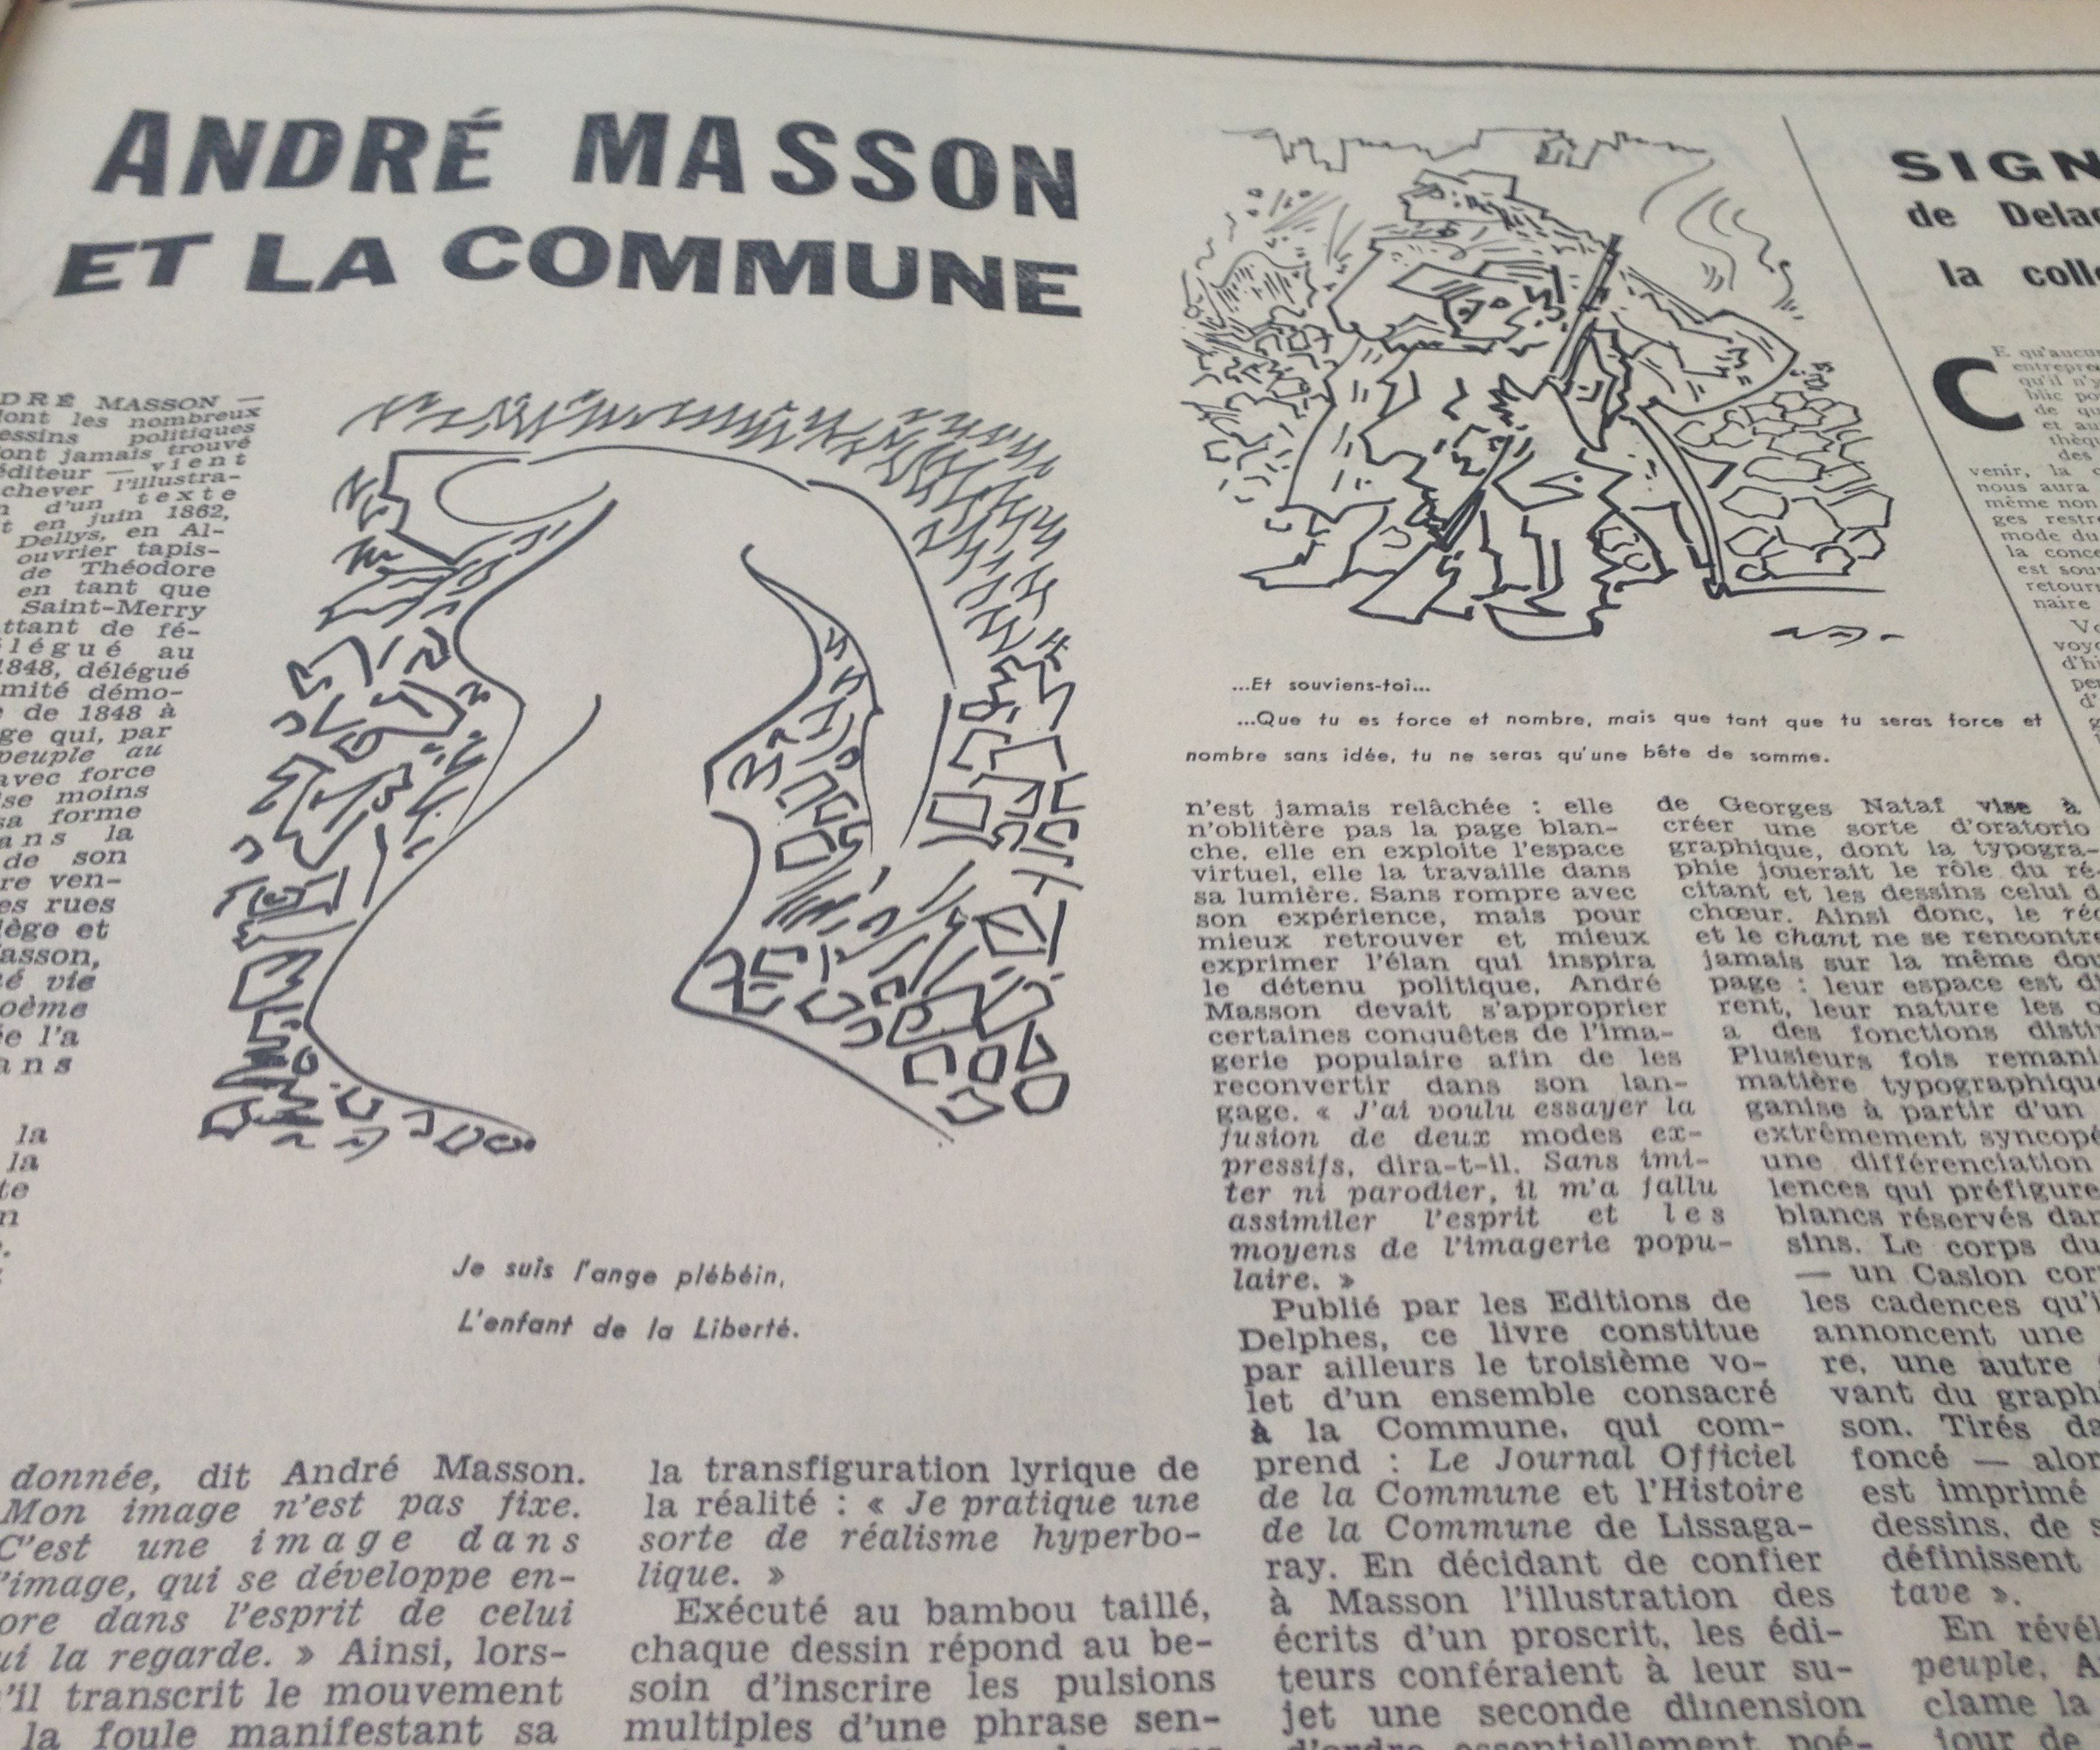
\includegraphics[width=0.33\textwidth]{massoncommune}
	\caption{\cite{commune}}\label{articlemoulin}
\end{figure}


 Antérieur à la fameuse période de la Commune de Paris de 1871 indiquée dans le titre, ce poème de 1862 est  placardé dans les rues de Paris pendant la Semaine Sanglante du 21 mai 1871. Cette pratique d'expression est courante chez les Parisiens pendant la Commune : Les textes placardés percutent comme des slogans introduits dans la vie du peuple qu'est la rue. Théodore Six a d'ailleurs un profil communard typique, c'est-à-dire que ce poète est aussi un artisan de condition sociale modeste. Sans oublier son passé de révolutionnaire avant la Commune au moment de la Révolution de 48.  Moulin rappelle ainsi le riche passé politique de Six, avec notamment un Coup d’Etat qui lui a valu le bagne en Algérie au moment de l'écriture de ce poème, le critique d’art Moulin relève la « force » de ce dernier tirée d’une \enquote{franche simplicité du discours}. On retrouve dans le lexique du critique l’élan patriotique des Parisiens qui prennent le fusil pour défendre leur ville et leurs idéaux républicains face à l’armée versaillaise de Thiers et ses représentants monarchistes. Le critique clôt ce paragraphe introductif et historique avec les mêmes termes du dessinateur et peintre André Masson sur son rapport à la Commune : \enquote{la Commune a donné vie à un authentique poème d’agitation.}

	  Ainsi, illustrer le poème \emph{Le peuple au peuple} reviendrait à amplifier sa valeur de révolution populaire, et lui donner image perpétuerait le mouvement insurrectionnel des Communards. De manière étonnante, on retrouve également l'expression du \emph{Mouvement perpétuel} d’Aragon et la force subversive présupposée de ce mouvement infini. Or, ce même mouvement, prêté par Masson à la Commune, est également celui qui \enquote{l’a constamment guidé dans son travail}. Ainsi, de même que \emph{Le peuple au peuple}, les oeuvres de Masson semblent puiser leur force dans l’élan, le mouvement pur, le mouvement comme signe. 

	Le second paragraphe insiste sur la pauvreté des témoignages des écrivains et des artistes au sujet de la Commune. Si, de la part des écrivains, cela peut s’expliquer par le fait qu’une majorité d’entre eux était hostile aux Communards, cela peut paraître plus étonnant du côté des artistes, puisque les semi-marginaux prenaient une part active aux événements aux côtés de la petite bourgeoisie (dans laquelle on retrouve Théodore Six). Même de la part d’un grand représentant tel que Courbet, à la tête de la fédération des artistes, Masson n’a connaissance que de \enquote{quelques croquis de Courbet et un ignoble livre de Gustave Doré contre les Communalistes}. 

    Le choix d’illustrer cette révolution populaire souligne donc la volonté du dessinateur de réhabiliter cette part de l’Histoire afin de la préserver du risque d’oubli. Mais la seconde moitié du paragraphe ouvre sur un second sujet plus riche en sources, celui du rôle des femmes sous la Commune : 

\begin{quote}
En revanche, la première héroïne dont j’ai entendu parler dans mon enfance, ce n’était pas Jeanne d’Arc mais Louise Michel. Ma mère était une admiratrice passionnée de Louise Michel.	
\end{quote}	
	
	Avec cette référence, Masson se situe dans un geste de transmission, à l’image de celui de sa mère qui l’a directement sensibilisé à cette période historique. Il se fait par le biais maternel lui-même enfant d’une Louise Michel. On conçoit ainsi que l’histoire de la Commune passe d'abord chez Masson par la transmission familiale des forts idéaux républicains de Louise Michel, mais l'on devine peut-être aussi l’héritage de son geste transgressif. L'héritage familial est poursuivi jusqu'en 1964 avec ses illustrations du poème de Six et surtout le livre \emph{André Masson et la Commune}. On peut également pressentir quelle influence a pu jouer le passé surréaliste dans l'évolution de Masson sur son imaginaire autour de la Commune.  Si Masson est d’une génération qui n’a pas vécu la Commune, né une vingtaine d’années plus tard, l’imaginaire autour de cette révolution populaire se forme d’abord grâce au témoignage maternel, se poursuit avec son attachement en tant qu'artiste pour les artistes-artisans et cet entrelacement de la création et de l'implication des révoltes sociales, pour arriver à se poser en 1964 comme commentateur de la Commune. Avec ses illustrations, sa voix s'entremêle et poursuit l'héritage collectif d'une histoire telle que la Commune qui risque plus encore que d'autres révolutions à tomber dans l'oubli, n'étant revendiquée et rappelée que par la partie gauche de l'échiqier politique et farouchement haïe par d'autres, comme en témoigne la question du nombre d'excéutions toujours énigmatique de Communards par les soldats Versaillais. Ainsi, illsutrer la Commune est une marque d'identité idéologique plus caractéristique et précise que ne le serait le même travail pour la Révolution Française, beaucoup plus unanimement célébrée. 


    C’est pourquoi Moulin ouvre son troisième paragraphe sur le rapport de Masson à la femme : \enquote{La République est femme; elle enfante les hommes}. Ainsi, à l’image de Louise Michel, la femme incarne pour Masson le mouvement subversif qui défend ses idéaux. Le mythe autour de la \enquote{Vierge Rouge} est clairement revendiqué. Celle-ci dépasserait même l’égalité avec l’homme pour lui être supérieure, puisqu’elle l’\enquote{enfante}. Pour autant, cette « fonction symbolique ne la prive pas de sa perspective réelle : elle tient sa place sur les barricades ou dans les ruines ». Or, c’est cette attitude révolutionnaire qui constitue pour Masson la beauté de la femme communarde. Masson les décrit comme membres du peuple dont le geste patriotique de prendre le fusil à la Place Blanche pendant la Semaine Sanglante en fait des combattantes égales aux hommes. Il n'est pas étonnant de la part de Masson de constater que son imaginaire autour de la Commune met la place de la femme communarde au centre, et que celle-ci le fascine de même que l'artiste-artisan : Cette image de la femme comme héroïne poursuit son prore travail artistique où la femme est une figure centrale, où la féminité est abondamment traquée. Ainsi, cette féminité qui fascine tant  Masson dans son art trouve l'une de ses inspirations chez les Parisiennes communardes combattantes. 

    Ainsi, la femme sous la Commune est comparée dans l’article de Moulin à l’idée de mouvement : \enquote{une même arabesque la décrit et l’environne, la liant à l’action dont elle émerge en armes}. Cette métaphore graphique du cycle montre la correspondance des idéologies défendues par ces femmes et leur mouvement insurrectionnel, ce qui justifie l’inspiration qu’elles procurent aux illustrations de Masson, où la forme incarne les idéaux. Ainsi, à partir de ce mouvement, Masson en retrouve d’autres analogues, tels « la guerre d’Espagne, ne voulant jamais suivre le texte à la lettre ni se laisser fermer dans l’anecdotique ». Cette autre guerre civile, de 1936 à 1939, peut faire écho à la Commune sous divers points, notamment en raison des combats républicains contre les nationalistes. L’échec des républicains qui donne lieu à la dictature de Franco est d’autant plus emblématique que, cette fois, Moulin précise la présence de Masson durant la guerre, \enquote{si bien que toute figure dressée dans la lutte implique graphiquement tout un peuple}: l’unité du peuple est illustrée chez Masson par la représentation d’un de ses membres qui les symbolise tous. Au nom certainement d’une autre représentation de Masson, \enquote{l’ange Liberté} dont \emph{une blancheur inaltérable, préserve sa puissance mythique de la réalité qui l’assaille}. On comprend par cette pureté symbolique de la Liberté qu’il s’agit pour Masson d’une valeur universelle à défendre communément pour tous les peuples, époques et lieux confondus. 


Le critique d'art Moulin illustre ainsi comment, à partir des idéaux défendus dans les illustrations du livre de Masson, la forme graphique prend forme et mouvement dans le dessin même. Avec l'entremêlement de son discours et la place qu'il laisse au discours rapporté de Masson, une polyphonie émerge de l'article entre le critique et l'artiste, notamment au niveau du registre du discours : le reistre esthétique est parcouru tour à tour par le topos lyrique mais aussi par le topos du mouvement au sens large du terme y compris violent qui rappelle sa nécesité dans la révolte sociale. Masson évoque une mise en abyme :\enquote{Mon image n’est pas fixe. C’est une image dans l’image, qui se développe encore dans l’esprit de celui qui la regarde}. Ainsi, le mouvement échapperait à son propre créateur selon celui qui le regarde, ce qui montre la volonté subversive des dessins : \enquote{Je pratique une sorte de réalisme hyperbolique}.Le fait que cette formule quasiment antithétique ne soit suivie d’aucune précision montre sa volonté de jouer sur une forme d’ambiguïté. On est plus proche de l’\enquote{art romanesque} selon Aragon que du réalisme balzacien, c'est-à-dire que Masson peut emprunter la conception aragonienne d'\enquote{d'aventure de l'esprit} : Masson confirme que ses dessins joints à l'article \emph{a priori} inspirés par une période historique n'ont pas pour vocation à être mimétiques. C'est l'esprit communard que Masson cherche à figurer, c'est-à-dire un esprit pris dans le vif des événéments brûlants et de l'action virulente. Ce n'est donc pas l'individu communard en tant que tel que Masson dessine, mais l'esprit révolutionnaire. Ce qui explique en partie pourquoi les dessins évoquent des esquisses pour la nature inachevée qu'ils inspirent, et pourquoi le trait est privilégié à la chair. 


	Au mouvement caractéristique des illustrations répond dans un effet-miroir sa technique, le \enquote{bambou taillé}, un type d’encre : \enquote{chaque dessin répond au besoin d’inscrire les pulsions multiples d’une phrase sensible, aussi diverse dans ses cassures que dans ses attaques}.Les dessins sont donc pour Masson un moyen d’exprimer fidèlement la force subversive du poème. Or, plutôt que la violence, c’est le lyrisme qui est réhabilité lorsque Moulin évoque une \enquote{tension mélodique}. Pourtant, ce lyrisme est réhabilité graphiquement par les illustrations, \enquote{pour mieux retrouver et mieux exprimer l’élan qui inspira le détenu politique}. 

Le lyrisme, graphique d'une part mais largement retranscrit dans le discours entrmêlé de Moulin et Masson, est bel et bien entremêlé à la dimension insurrectionnelle du poème. C’est ce même croisement qui inspire les dessins dans un souci de fidélité à l’esprit du poème, et à travers l’esprit de révolution populaire. La violence présupposée, la beauté insurrectionnelle s’exprime au contraire par le lyrisme, \enquote{sans imiter ni parodier, il m’a fallu assimiler l’esprit et les moyens de l’imagerie populaire}: si l’expression graphique de Masson témoigne de sa vision personnelle des événements, c’est aussi par souci de réhabilitation du regard sur les événements, où il s’agit de donner vie. Mais cette réhabilitation demande néanmoins selon le dessinateur de passer par une connaissance autant des états d’esprits de l’époque que de leurs images, à partir desquels seulement l’artiste livre son regard mouvant. 

%Mettre illustrations de Masson 

Par ailleurs, puisqu’il s’agit d’un troisième volet dédié à la Commune, Moulin précise la dimension poétique du livre prodiguée par les illustrations de Masson. La dimension lyrique se retrouve dans la mise en page de Nataf, disposée comme une chorale, 
\begin{quote}
une sorte d’oratorio graphique, dont la typographie jouerait le rôle du récitant et les dessins celui du choeur.\end{quote}

 Cette division permet d’introduire une rythmique de l’espace, entre la typographie et le blanc de la page. Moulin évoque même 
 \begin{quote}
le corps du caractère — un Caslon corps 20— et les cadences qu’il détermine annoncent une autre lecture, une autre couleur dérivant du graphisme de Masson. 	 
 \end{quote}

 On peut ainsi apercevoir dans la forte présence musicale des dessins et de la mise en page une évocation lyrique de la Commune incarnée par le compositeur Jean-Baptiste Clément. 

L’image d'\enquote{une autre octave} semble chercher à retrouver sur le papier la musicalité du compositeur de la Commune. De même, l’allusion appuyée par l’italique de la \emph{couleur} induite dans les dessins de Masson semble figurer symboliquement le \enquote{rouge cerise} emblématique du lyrisme de l’histoire de la Commune. Le choix du lyrisme à part entière est donc déterminant dans cette lecture voulue poétique de l’histoire de la Commune. 

Pour illustrer la critique de R.J. Moulin, deux dessins de Masson avec des légendes tirées du poème encadrent les paragraphes.  Le dessin de gauche illustre des vers dans la partie \emph{Le rêve du poème}, \enquote{Je suis l’ange plébéien / L’enfant de la Liberté}. On reconnait grâce à la légende le fameux ange de la Liberté évoqué par le critique. Le dessin illustre un corps aux multiples courbes.Au lieu de voler dans les airs, l’ange en question semble allongé dans un univers réaliste : on identifie la forme des touffes d’herbes et la forme de feuilles d’arbres. L’ange n’a d’ailleurs pas d’ailes, et sa tête sans visage a le cou courbé vers l’herbe. La courbe de son corps,le trait inachevé de la tête et les lignes des doigts se complètent avec les brindilles d’herbes et de feuilles. Ainsi, cet ange comme symbole du peuple fait corps avec la nature dans une parfaite harmonie. Au lieu d’arrêter le mouvement de la nature, les traits du corps semblent suivre leur élan, tout en étant dans une attitude de repos qui montre sa tranquillité d’esprit.

% Image : Dessin de l'article 

Le poème aligné en haut à droite de l’article illustre la partie  \emph{Remember!} du poème, avec pour légende :\enquote{…Et souviens-toi…/…Que tu es force et nombre, mais que tant que tu seras force et / nombre sans idée, tu ne seras qu’une bête de somme}. Ces vers à valeur de maxime pouvaient à l’époque de la Commune paraître comme une main tendue vers les Provinciaux. Ces derniers s’opposaient à la Commune en se réclamant de la paix. Seulement, dans l’esprit des Communards, il s’agissait en réalité de défendre les mêmes idéaux de classes modestes qui combattent pour leur terre et le travail.

Ce lyrisme patriotique est illustré par Masson avec deux protagonistes au coeur du dessin. Celui debout à la gauche du lecteur semble porter un chapeau de paille et des vêtements modestes. A ses côtés, un personnage agenouillé avec une casquette, des bottes et des épaulettes tient un fusil. On peut y voir ainsi la représentation du paysan à côté du soldat. La cause de l’homme de la terre et celui de la ville, peut-être un représentant de la garde nationale, est unifiée. A l’arrière plan, on trouve une ligne de bâtiments qui évoque des barricades. Deux chemins y mènent respectivement, l’un partant du côté du paysan, l’autre de celui du soldat. Bien que le mouvement des traits paraisse plus discernable que les formes représentées, on reconnaît la forme des pavés qui mènent jusqu’aux barricades.
%image n2

 Malgré le mouvement du décor avec un chemin ponctué de multiples traits, les deux personnages semblent attendre : le paysan a les bras croisés et le soldat ne se sert pas de son fusil pour tirer, même si sa position le représente en alerte dans une attitude de défense. Sur le chemin de gauche, une forme de rechange courbée semble représenter un visage de femme. Sa tête en forme de drapeau rassemble autour d’elle de multiples traits, ainsi qu’à l’intérieur du drapeau, et des envols de petits cailloux au-dessus de sa tête. Mais le côté droit du drapeau n’est pas complètement fermé. Ainsi, cette femme-drapeau semble s’adresser directement aux deux personnages. On peut y reconnaître la représentation de la République en femme caractéristique de Masson. C’est pourquoi les deux personnages unis, la distinction des traits de leurs corps respectifs est peu discernable, affichent une attitude plus de défense que d’attaque. Leur comportement protecteur pour le soldat et songeur pour le paysan illustre la légende basée sur l’importance du mouvement perpétuel de la pensée du peuple. 

 Le croisement dans cet article de Raoul-Jean Moulin des témoignages intimes de Masson vis-à-vis de la Commune et de ses esquisses révèle quelle valeur éducative a été dans sa philosophie et son esthétique un tel événement. La Commune, que l’on soit du côté des Parisiens ou des Versaillais et Provinciaux, est ressentie comme la libération la plus totale du peuple, y compris au sens du libertinage avec le retour du peuple à ses instincts primaires. Valorisée par les communards ou condamnés après la Commune par ses ennemis, la libération des corps et des moeurs est son élément particulier qui la distingue des autres insurrections. C’est pourquoi la Commune ne peut que naturellement s’imbriquer dans l’idéologie de Masson, et l’on sait combien le mot « révolution » revient fréquemment, comme martelé, dans ses correspondances, et que celle-ci est aussi proprement physique. C’est donc aussi une influence proprement esthétique que joue sur André Masson un exemple de liberté absolue des expressions du peuple avec lequel Masson choisit clairement de se confondre. 

\subsection{La sensiblité communarde d'Aragon}

D'autre part, si Aragon et Masson partagent une sensibiltié autour du thème de la Commune de Paris relève pourtant de profondes distinctions. Cette distinction serait probablement à situer à la mémoire après la Commune, c'est-à-dire à l'adhésion d'Aragon au Parti Communiste et aux réserves de Masson sur les théories marxistes. Autrement dit, la sensibilité d'Aragon vis-à-vis de la Commune de Paris se situe dans l'héritage de l'histoire du communisme, et, plus particulièremet, à la conception de la Commune comme l'événement qui engendrera la Révolution Russe d'Octobre 1917, rêve déjà présent dans les esprits des révoltuionnaires de 1917 et recensé par l'historien Jacques Rougerie : 

\begin{quote}
\emph{On sait que le révolutionnaire russe avait dansé dans la neige lorsque la durée du pouvoir des soviets eut dépassé de vingt-quatre heures seulement celle de la Commune de Paris, et qu’il dort, dans son mausolée, enveloppé du drapeau de l’un des bataillons de la garde nationale insurgée en 1871. Pour Staline encore, qui ici paraphrase Marx :} « La République des Soviets est la forme politique recherchée et enfin trouvée, dans le cadre de laquelle doit être réalisée l’émancipation économique du prolétariat, la victoire complète du  socialisme. La Commune de Paris a été l’embryon de cette forme. Le pouvoir des Soviets en est le développement et le couronnement.\footcite[p241]{proces}\end{quote}

La valeur défendue par Aragon du réalisme socialiste prend ainsi en compte l'héritage de la Commmune de Paris comme première pierre de l'édifice communiste, c'est-à-dire que le \enquote{réalisme socialiste} ne peut exister également qu'à partir de la Commune de Paris. Cette référence historique lui permet d'ailleurs de propager à la fois le réalisme socialiste et légitimer l'idéologie communiste en France : 

\begin{quote}
“Non, le type soviétique d’Etat n’est pas spécifiquement russe. Il est né de la Commune de Paris: il n’a pu se développer que grâce à l’expérience de la lutte de classe internationale, dont les bolcheviks ont su tirer les leçons. Mais dans son application dans l’U.R.S.S. même, il faut toute l’ignorance volontaire de nos démocrates bourgeois pour prétendre qu’il s’agit là d’une expérience spécifiquement russe.“\footcite[p121]{lavoinne}	
\end{quote}

Néanmoins, cet imaginaire romantique autour de la Commune est représenté dans l'esprit d'Aragon par la figure de Rimbaud. Ce choix n'est pas anodin, d'autant plus que, avec Lautrémont, Rimbaud avait été l'un des sujets d'affinités entre les jeunes médecins Aragon et Breton rencontrés sur le Front. Tout comme Rimbad figure parmi les grands noms dont se revendiquent le groupe surréaliste. Il est donc intéressant que Rimbaud accompagne Aragon tant à l'aube de la période dada, pendant l'époque surréaliste, et durant son engagement politique : \enquote{Aragon liera au nom de Rimbaud l’image de la révolte et du peuple insurgé de la Commune de Paris, et il retrouvera bientôt chez un grand nombre de peintres français le réalisme qu’il admire chez Cézanne et Courbet.}\footcite[p165]{these}

Aragon se passionnerait-il pour la Commune à partir de sa fascination première pour Rimbaud ? Toujours est-il que sa présence, comme celle de la Commune, attribuent une certaine forme subversise envisagée dans la vision du réalisme socialiste, en ce sens où le réalisme socialiste, en se positionnant du côté du peuple, se comporterait par nature comme un mouvement révolutionnaire :

\begin{quote}
Aragon explique (ibid., p. 241) :\enquote{On doit se souvenir de ce fait très simple qu’Arthur Rimbaud en 1871 était venu tout naturellement à Paris s’engager dans l’armée de la Commune. Ses poèmes de cette époque sont des poèmes à la gloire de la Commune. Que serait-il advenu de Rimbaud dans une Commune triomphante ? Nous l’ignorons, mais nous savons ce qu’il en est advenu, la Commune vaincue} : telle est l’interprétation marxiste de son fameux \enquote{silence}, une interprétation de plus.\footcite[p241]{these}	
\end{quote} 

En entremêlant la destinée de Rimbaud et celle de la Commune à la fin de celle-ci, Aragon livre un symbole fort : le poète, c'est-à-dire l'écrivain selon la conception réalsite socialiste, se situe parmi les membres du peuple dans le cycle révolutionnaire et son existence en tant que poète est ancrée dans celle du mouvement qui le soulève. C'est pourquoi le réalisme socialiste, (même si au premier abord l'idée peut paraître contradictoire avec la notion \enquote{réaliste} doit se concevoir) doit une atmosphère de lyrisme révolutionnaire. 

En outre, on peut soupçonner que le rapport d'Aragon vis-à-vis de la Commune, et peut-être plus encore comme le montre l'exemple de Rimbaud la proximité avec l'échec de la Commune, dépassent la thèse communiste et agit aussi comme un repérage historique dans un niveu plus intime : Dans \emph{Les voyageurs de l'Impériale}, le personnage principal, le grand-père Pierre Mercadier était présent pendant la Commune : 
\begin{quote}
 Il redoutait les aléas de l’avenir du monde. Il avait traversé des bouleversements, il savait au fond la fragilité de l’édifice social. Né en 1856, il avait passé son enfance dans le temps de l’Empire libéral. […] L’Empire était tombé, les Prussiens campaient un peu partout en France, il y avait eu la Commune, et Pierre Mercadier n’avait encore que quinze ans.\footcite[p43]{voyageursdelimperiale}\end{quote}

 Comme Rimbaud, le personnage Pierre Mercadier, inspiré en partie par le grand-père maternel d'Aragon, a neuf années de moins que la personne réelle Fernand de Biglione, de telle sorte qu'il vit la Commune adolescent et non pas adulte. Cette réflexion illustre l'atmosphère romantique qu'Aragon se fait de la Commune, conçue pour être vécue par son peronnage en pleine période d'émancipation, à un moment où la défaite de la Commune a un impact fodnateur dans cette période de transition qu'est l'adolescence. 

 Plus généralement, dans \emph{Les Voaygeurs de l'Impériale}, l'échec de la Commune agit comme un spectre, c'est-à-dire qu'elle agit comme un traumatisme pour les personnages les plus âgés du romans, tels que Pierre Mercadier ou l'oncle Blaise :

 \begin{quote}
 La France sortait d’un cauchemar prolongé. Les hommes nés pendant la guerre allaient avoir trente ans. Ainsi l’on atteignait graduellement à l’oubli de l’invasion. Le souvenir des luttes intestines demeurait plus vivace parce qu’à la Commune avaient succédé les bannissements, les ostracismes, parce que de la Commune était née une grande peur qui ne faiblissait pas au coeur de  ceux qui l’avaient tuée.\footcite[p459]{voyageursdelimperiale}\end{quote}

 Avec cette présence discrète mais persistante de la Commune à l'image d'un spectre dans tout le roman, Aragon dévoile ici une conviction à partir de l'échec de la Commune, qui serait celle d'une résurrection possible pour celle-ci, c'est-à-dire une revanche à prendre,celle du prolétariat sur la bourgeoisie. De telle sorte que la temporalité du roman est encadrée par la défaite de la Commune et la veille de la 1ère Guerre Mondiale. Or, cette vision temporelle ne s'explique pas uniquement d'après la perspective du réalisme socialiste, puisque l'on retrouve ces deux références historiques dans \emph{Blanche ou l'oubli}:

 \begin{quote}
Entre cet été pluvieux où Marie Noire sur la Côte mesure au peu d’entrain de son ami saisonnier que la jeunesse porte en elle sa fin et ces après-midi avenue Victor-Hugo chez Maryse, il y a le temps qui sépare la Commune de Paris de l’éclatement de la guerre en 14. Je me fais l’effet d’une vieille pendule qui ne s’est pas contentée de la durée des autres. Est-ce qu’en 1914 j’avais la moindre représentation de la vie à Paris en 71 ? Pourquoi le joueur de volley-ball devrait-il se faire une image exacte du Mouvement Dada ? ou du salon de l’avenue Victor-Hugo ?\footcite[p38]{blancheouloubli}\end{quote} 

Ainsi, la Commune n'est pas seulement un repère temporel, puisque, ancrée dans l'obsession plus génrale du temps chez Aragon dans ses oeuvres, la Commune est vue comme un élément romanesque. C'est d'ailleurs la transition du temps de la Commune qui semble fasciner Aragon: la défaite de la Commune, c'est-à-dire l'après les événements de la Semaine Sanglante, la transition. Mais la figure du Rimbaud adolescent comme celle de Pierre Mercadier conçoit la Commune vécue dans l'imaginaire romantique comme une période de transition, entre deux âges. Dans la conception romanesque d'Aragon et son rapport au temps, la Commune est un élément d'entre-deux. 
 
\subsection{La référence prépondérante de la Commune dans l'Histoire des \emph{Lettres françaises}}

Si la Commune joue un rôle dans la conception idéologique et comme marqueur temporel dans l'oeuvre d'Aragon, elle influence également son parcours journalistique, dans la lignée de celui de membre du Parti Communiste. En 1934, Aragon militant est rédacteur à la fois dans le journal \emph{L'Humanité} et dans la revue \emph{Commune}, pour laquelle Aragon est rédacteur pour la rubrique \emph{Les Livres}. En plus d'un titre à la référence transparente, la revue est dirigée en partie par Paul Vaillant-Couturier au nom de l'A.E.A.R (Association Des Ecrivains Révolutionnaires).\enquote{La Commune} sert donc à mentionner l'idéologie communiste, et en particulier à fixer la valeur révolutionnaire comme exigence de son discours, de ses débuts jusqu'aux \emph{Lettres françaises}.Le propre discours d'Aragon emprunte des voies différentes en fonction du type de public différent socialement pour qualifier le réalisme socialiste qu'il cherche à propager en France : 

\begin{quote}
 Sur le plan journalistique d’autre part on notera que \emph{Commune}, revue pour les intellectuels, utilise plus volontiers que \emph{L’Humanité} l’expression “réalisme socialiste“. Mais entre la revue et le quotidien, une identique volonté de lier politique et littérature conduit à une large communauté de vues.\footcite[p157]{lavoinne}\end{quote}

Ainsi, même en prenant en considération une éventuelle réception distincte de deux type de lecteurs, Aragon vise avant tout un choix de politique éditoriale qui n'est pas sans rappeler celui à venir des \emph{Lettres françaises} : bien qu'il s'agisse avant tout d'un journal culturel,le propos politique est ancré dans la critique :

\begin{quote}
 L’activité du public lui apparaissait comme le plus sûr gage d’amélioration d’une revue qui “n’est pas sans défauts: ses numéros n’ont pas toujours l’équilibre souhaitable, et ce n’est que récemment,  et d’ailleurs sous le feu de la critique de son public, qu’elle a su vraiment organiser sa partie la plus vivante, ses chroniques qui vont de l'actualité des livres, du cinéma à celle des journaux et de la rue, de la vie même.“ On notera ici que l’ancien surréaliste et le journaliste s’alliaient chez Aragon pour faire sortir une revue intellectuelle des sentiers battus du débat théorique pour flairer le vent de l’éventuel, humer l’air du temps au-delà des frontières de l’imprimé.\footcite[p205]{lavoinne}\end{quote}

Ces quelques lignes laissent déjà pressentir son projet éditorial pour \emph{Les Lettres françaises} lorsqu'il en prend finalement la direction en 1953. On remarque d'ailleurs que, au service de la revue, l'imaginaire communard ne joue pas sur les mêmes aspects que plus tard dans les romans. De telle sorte que, au contraire de la défaite, Aragon cherche justement à redonner vie à l'esprit communard aussi bien dans \emph{Commune} que dans \emph{L'Humanité}:  

\begin{quote}
 Avant de tenter d’expliquer le comportement d’Aragon, il est nécessaire de compléter le tableau qu’il brossait de l’Union soviétique. En 1935, à son retour en France, il la célébra à l’occasion du 64ème anniversaire de la Commune de Paris dans une page spéciale de L’Humanité (17 mars 1935) : \enquote{Vive la Commune}. 
Le thème de la Commune permettait de réaffirmer le lien privilégié entre les prolétaires français et soviétiques. Comme tous les théoriciens marxistes, Aragon souligne en effet la relation entre l’insurrection parisienne de 1871 et la Révolution d’Octobre.\footcite[p133]{lavoinne}
\end{quote}

Ressuciter la Commune par un titre d'article voulu comme un cri,illustre le projet politique plus global d'Aragon et plus généralement de l'A.E.A.R. de renverser les valeurs bourgeoises par les idéaux révolutionnaires, en particulier en ce qui concerne les écrivains. Que cette commémoration paraisseà l'occasion de cet anniversaire dans \emph{L'Humanité,} un journal plutôt adressé aux ouvrirers implique  que non seulement le Parti Communiste se fait leur représentant, mais surtout qu'il ambitionne de leur réattribuer l'esprit communard. Le modèle révolutionnaire tel que le conçoivent Aragon et Paul Vaillant-Couturier derrière l'A.E.A.R. 

Cette pratique des anniversaires, d'évenements forts ou de grands noms culturels et politiques, demeurera dans \emph{Les Lettres françaises} une marque de fabrique,avant la direction d'Aragon, mais peut-être plus souvent encore sous celle-ci. La Commune est parmi les anniversaires récurrents, et, dans les dernières années de la direction de Claude Morgan, lorsqu'Aragon dirige en novembre 1951 la nouvelle rubrique \emph{Tous les Arts}, en pleine année d'anniversaire de la Commune, la commémoration est poursuivie, après d'importantes pages publiées auparavant en mars et en mai jusqu'à en faire des sources documentaires conséquentes. Le directeur de l'époque, Claude Morgan quant à lui s'inscrit dans un rapport à l'insurrection plus proche de la Révolution Française en convoquant la figure du révolutionnaire et proche de Robespierre Saint-Just :

\begin{quote}
Claude Morgan se référait à Saint-Just (dans son article du 9 septembre 1944) pour condamner toute indulgence ; un an plus tard, il use du même langage pour dénoncer \enquote{l'esprit de trêve} et exhorter \enquote{les honnêtes gens} à \enquote{reprendre celui du combat} en s'opposant à la \enquote{conjuration} des modérés : \enquote{chaque assassin gracié est un coup en pleine poitrine de l'innocent [...] un pas de plus et vous pouvez ouvrir la porte à Montherlant, à Giono.}\footcite[p538]{these}	
\end{quote}

\begin{figure}[H]
   \centering
   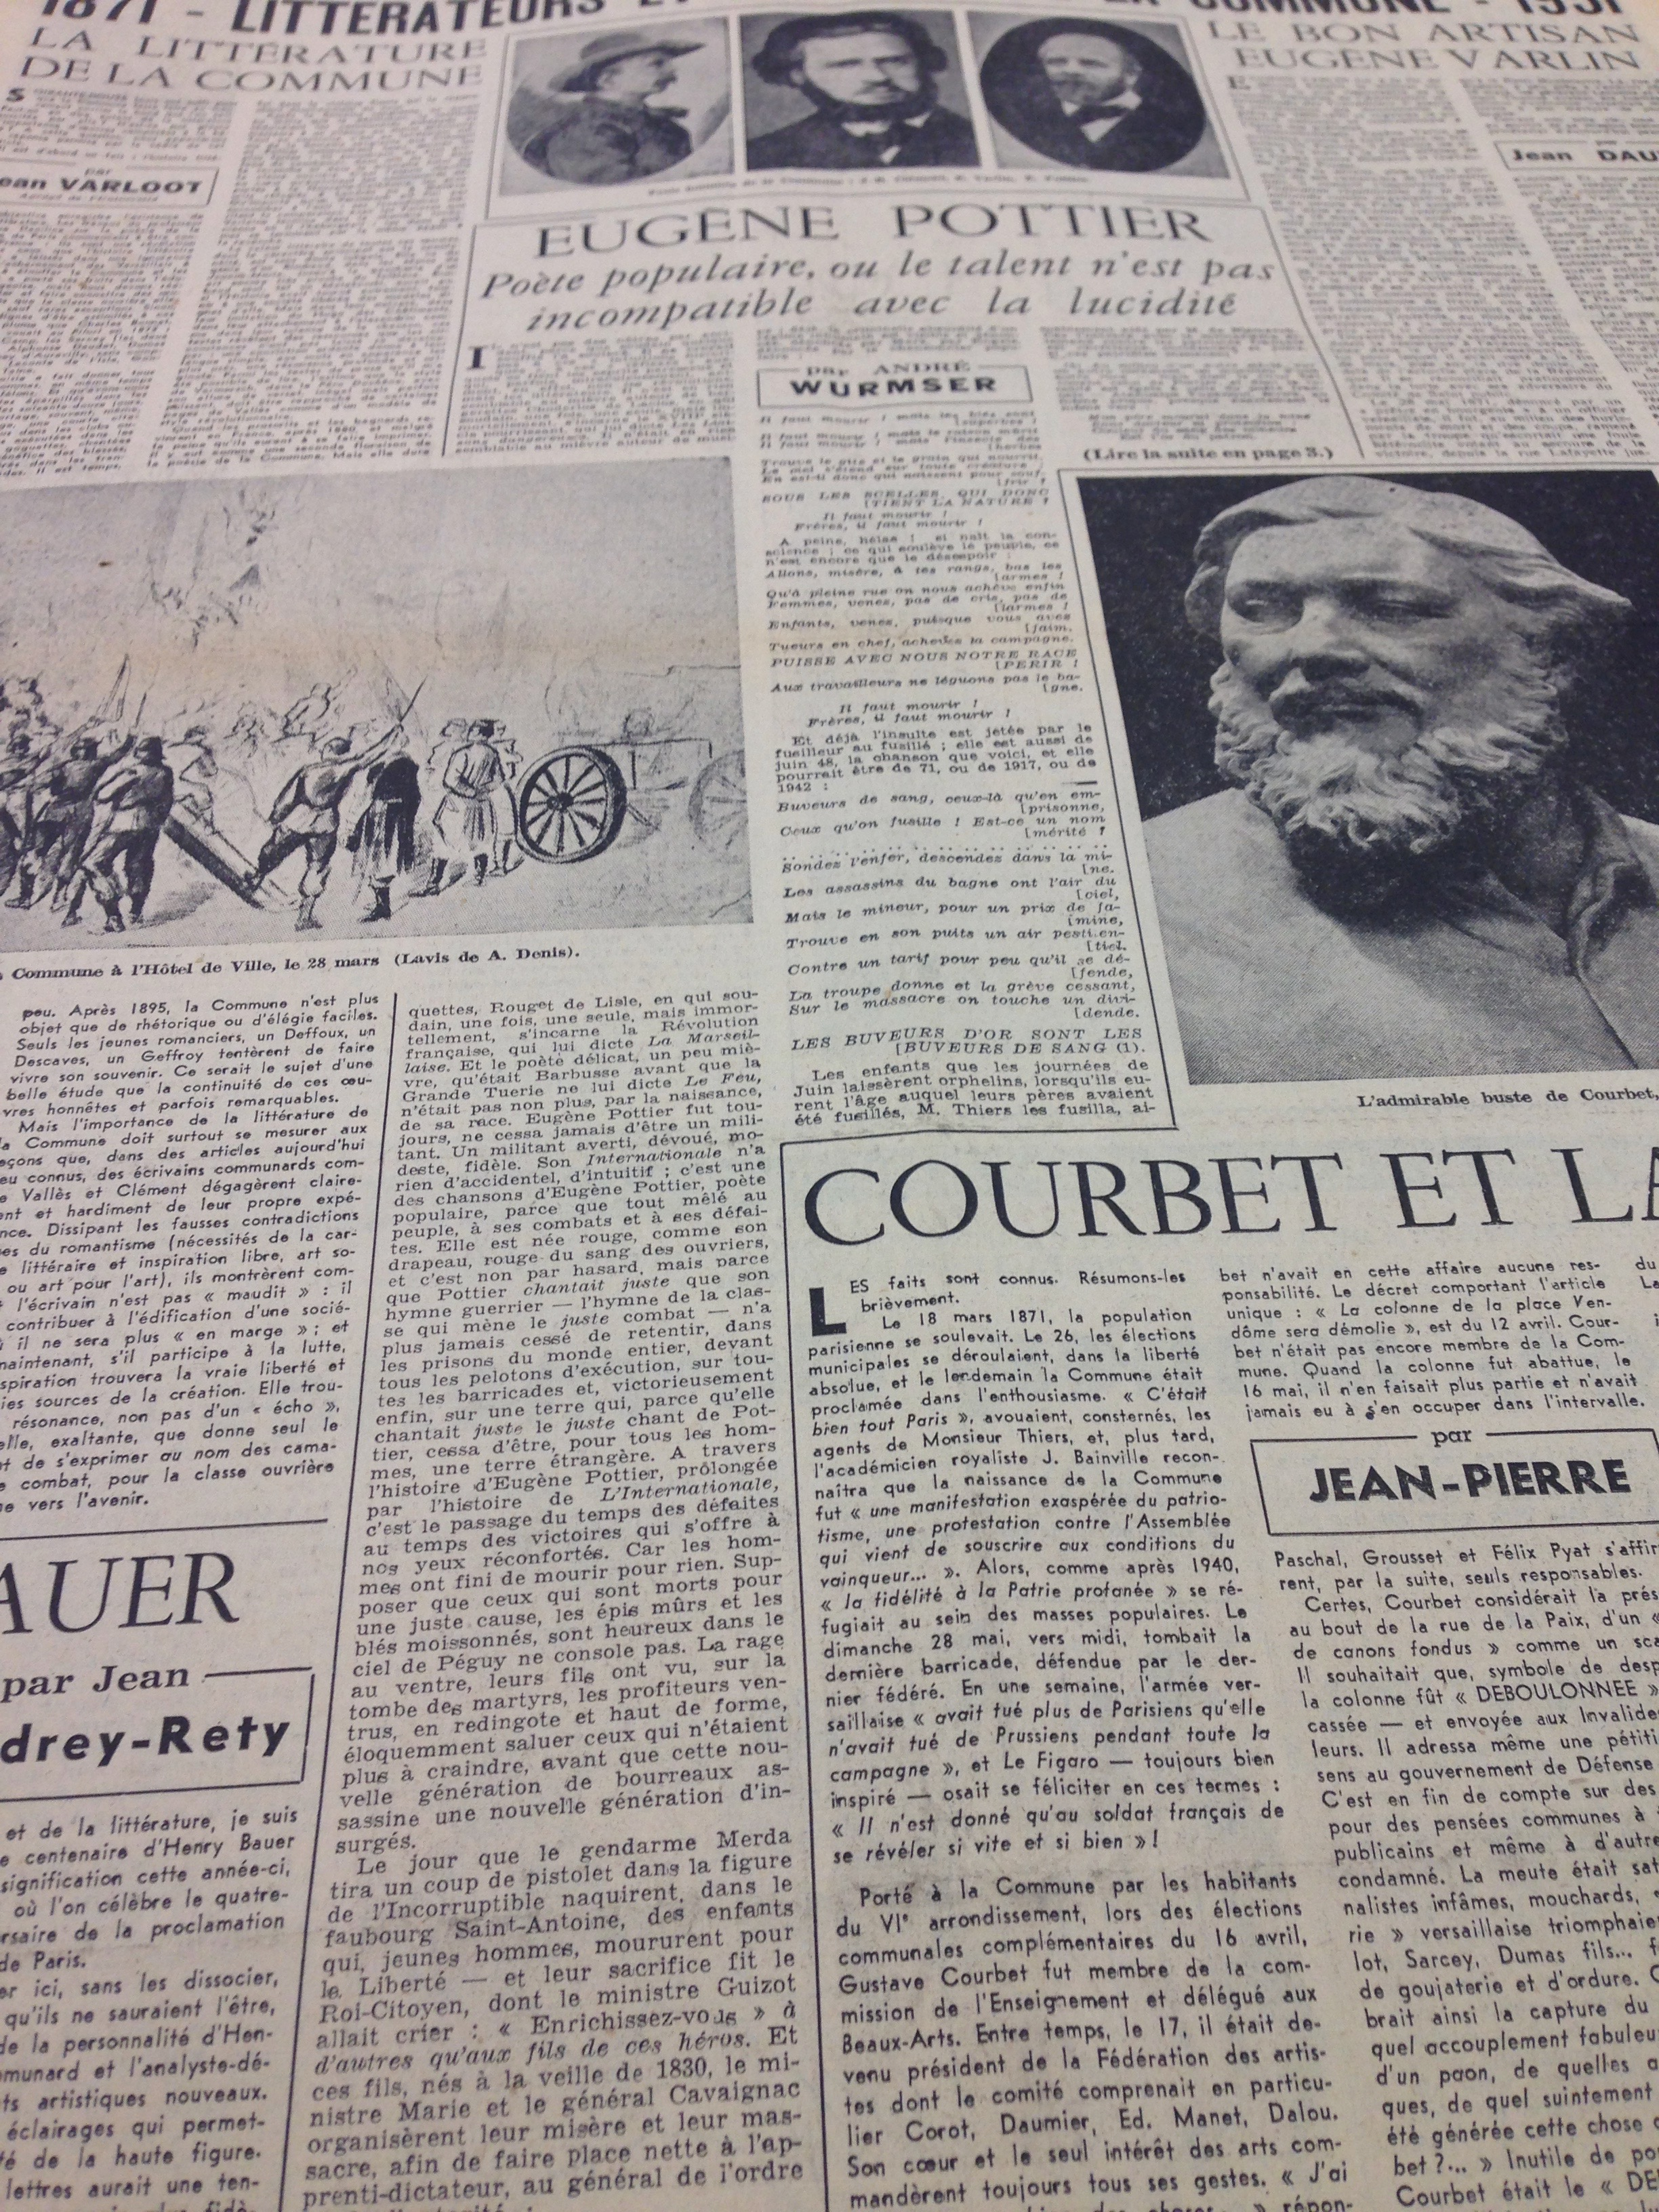
\includegraphics[width=0.33\textwidth]{courbetcommune}
	\caption{\cite{courbetcommunard}}\label{courbetcommune}
\end{figure}

Ainsi, dix ans après s article de 1944, un mouvement insurrectionnel tel que la Commune ne sert pas exactement le même projet politique que celui du renversement des valeurs idéolgiques au temps de \emph{Commune} et \emph{L'Humanité} dans les années 34-36. Or, un journal comme \emph{Les Lettres françaises} né sous la clandestinité, fait de la Résistance à la fois son héritage et son mot d'ordre politique. Ainsi, les quatre-vingt ans de la Commune en 1951 servent un modèle de résistance, c'est-à-dire dans un sens plus large que celui de la défense de la cause ouvrière. Dans le premier article qu'il écrit dans la rubrique \emph{Tous les Arts} en novembre 51, Aragon publie un texte conséquent, \emph{Peindre a cessé d'être un jeu} dans lequel l'exemple de Courbet communard sert d'exemple de peintre voué à la cause du \enquote{sentiment national}. Aragon écrit cet article en faisant référence à un fait d'actualité arrivé au Salon d'automne, pendant lequel sept tableaux du vernissage,sont retirés de l'exposition au moment de la visite présidentielle avec pour justification le \enquote{sentiment national}. Aragon, scandalisé par l'aspect \enquote{arbitraire} caché derrière le noble sentiment revient sur de grandes époques et de grands noms de la peinture à travers les siècles pour donner son conception du \enquote{sentiment national} : 
 
\begin{quote}
Quant à Courbet, ah! Courbet, un homme injurié, honni, condamné, traqué, exilé...Bien sûr, les Baylot d'alors ne l'aimaient pas, mais il fallut lui inventer l'histoire de la colonne Vendôme pour lui faire son affaire.[…] Les jeunes gens, même adonnés aux expériences les plus folles, aux rêves de la couleur et du trait, auront, désormais, devant les yeux, cet interdit du mensonge, comme aux jours de Vichy, quand nous écrivions, à chaque abandon au délire, à chaque mot risqué, nous nous rappelions ce qui était le feu véritable, et les héros dans les prisons et devant les pelotons d'exécution, les mots s'ordonnaient, suivaient un penchant tout autre, se gorgeaient du réel, du \emph{sentiment national}. 	
\end{quote}

Ainsi, par la référence à l'un des plus épisodes de la Commune autour de la Colonne détruite alors que Courbet présidait la Fédération des Artistes, Aragon conteste d'abord la responsabilité de Courbet dans cette affaire, mais surtout il réhabilite l'image du peintre qui résiste en s'engageant dans la Garde Nationale pour défendre la ville de Paris. C'est donc une autre persective qu'Aragon aborde vis-à-vis de la Commune, celle de la défense à la fois de la ville et des causes idélogiques en train de germer au sein des classes parisiennes modestes. Mais la lutte des classes n'est plus tant la question, puisque l'image du peintre Courbet défendant les barricades est avant tout une image de liberté, probablement l'autre terme qui se cache derrière le mot d'ordre de Résistance. 



\section{De la Commune à la Résistance, ligne directrice des \emph{Lettres françaises} 

\subsection{André Masson, médiateur entre Elsa Triolet et la Résistance}

\begin{figure}[H]
   \centering
   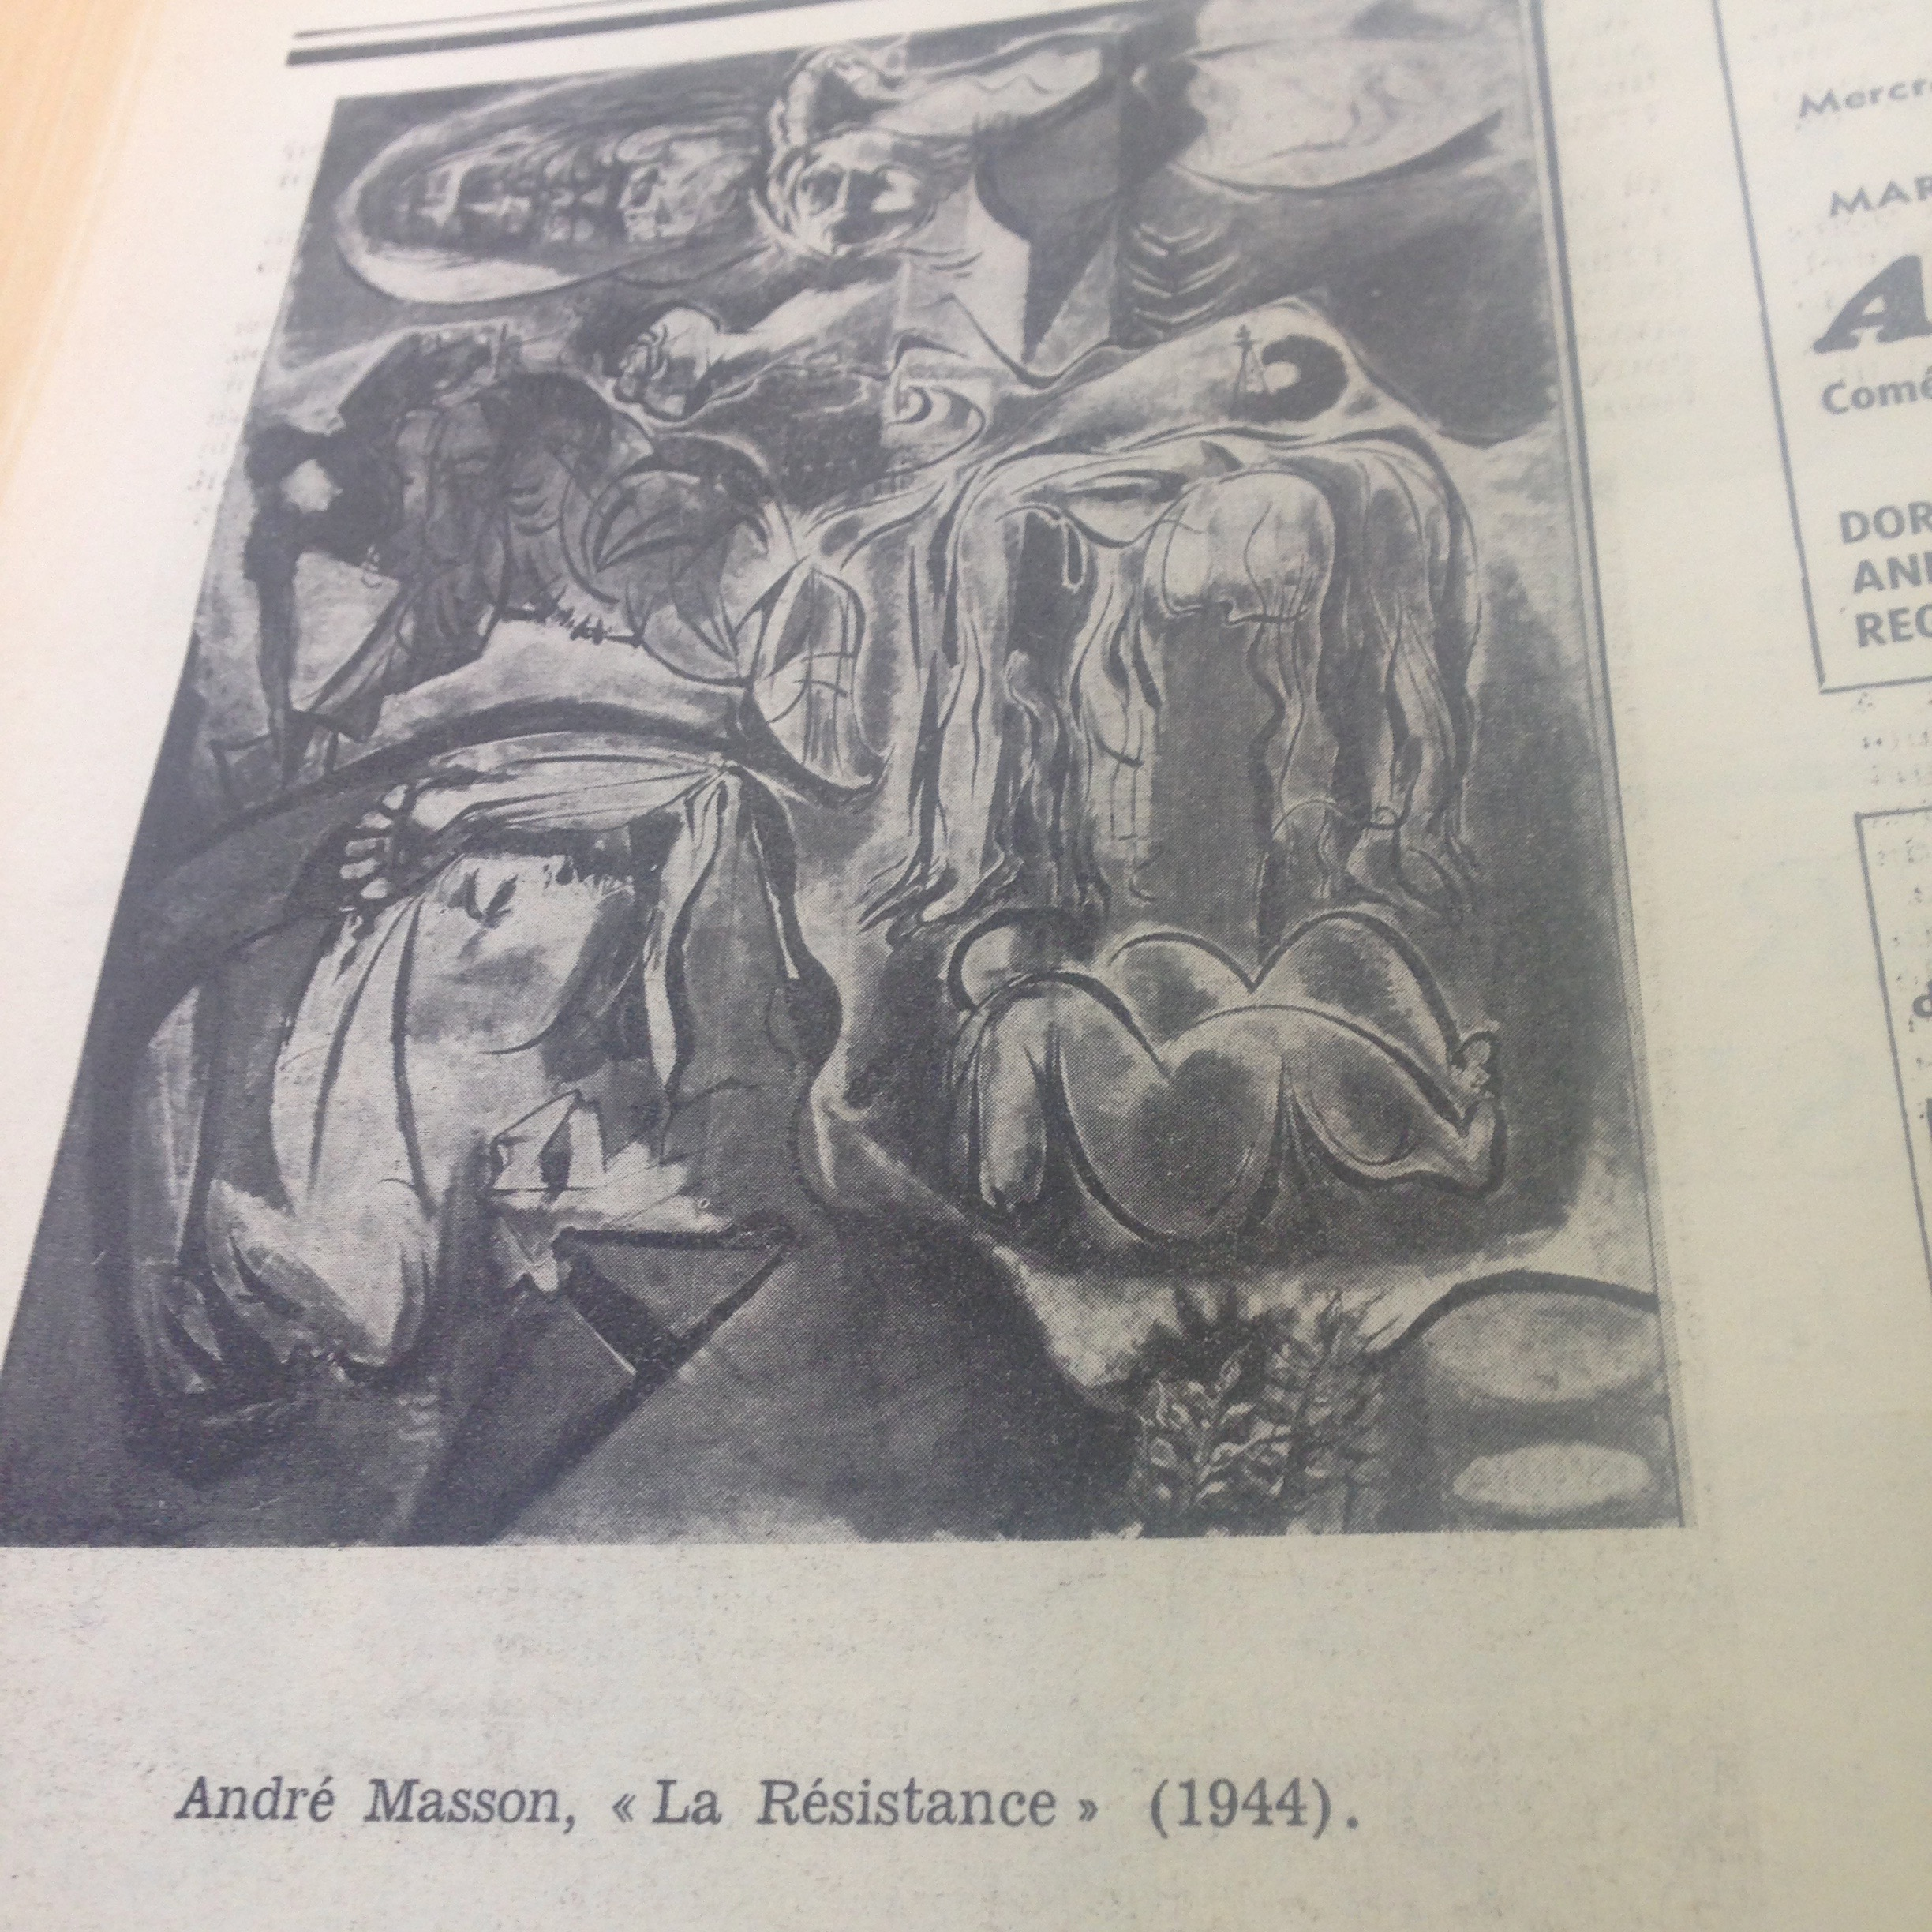
\includegraphics[width=0.33\textwidth]{resistancep2.jpg}
	\caption{\cite{specialelsa}}\label{fig:Réssitance}
\end{figure}

\begin{figure}[H]
   \centering
   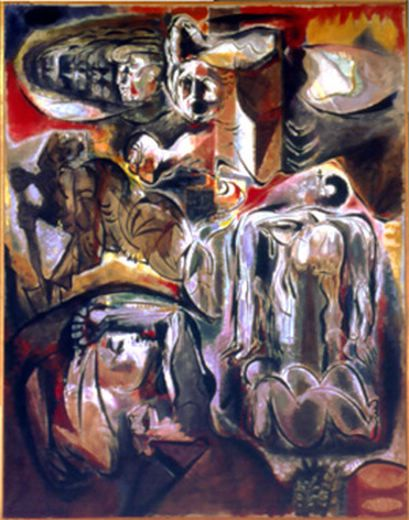
\includegraphics[width=0.33\textwidth]{resistancecouleur.jpg}
	\caption{\cite{specialelsa}}\label{fig:Réssitancecouleur}
\end{figure}



Or, si la Commune est un sujet fidèle et récurrent dans l’ensemble des années des \emph{Lettres françaises}, célébrée à chaque chiffres ronds, mais pas uniquement au moment des anniversaires, et que répertorier les articles sur le sujet conduirait à de riches ressources historiques,l’imaginaire insurrectionnel sous-entendu par cette période historique conduit à un autre terme qui figure le mot d’ordre du journal. \emph{Les Lettres françaises} naît pendant la Résistance. Il est conçu comme un outil intellectuel au service de cette période spécifique qu’est la Résistance. On peut ainsi concevoir qu’un journal qui doit son existence tout entière à ce moment de l’Histoire et la nature subversive de celui-ci, devenu un passé glorieux après la guerre, fasse du mot « Résistance » la ligne directrice du journal, étant le maitre-mot de sa politique. 


	Ce choix éditorial soulève en lui-même beaucoup de questions, à commencer par l’évolution de la signification du mot \enquote{ésistance}hors l’organisation spécifique de groupes clandestins destinés à s’opposer aux actions de Vichy et des Nazis. C’est la période où André Masson découvre depuis les Etats-Unis \emph{Les Lettres françaises}, dès les premiers numéros, puisqu’il y  fait allusion dans ses correspondances à des articles de 1942. Aussi écrit-il à l’écrivain Roger Caillois : \enquote{J’ai lu votre très beau texte : “La Pampa“ dans le dernier numéro que j’ai reçu des L.F- Si cette revue ne paraît plus ce sera désolant. (Lettres françaises, n\degre 4, 1er avril 1942, pp. 1-3).}\footcite[p482]{anneessurrealistes} André Masson, comme l’un de ses premiers lecteurs noue donc immédiatement malgré la distance géographique un rapport intime et fidèle aux emph{Lettres françaises}. 


	Aragon, de son côté, participe à sa naissance en opérant la rencontre entre ses premiers dirigeants, Jacques Decour et Jean Paulhan. Par la suite, on s’aperçoit vite que l’évolution du terme \enquote{résistance}, même s’il reste clairement le mot d’ordre, dépend bien sûr des événements historiques à venir, mais aussi de ses dirigeants. Ainsi, lorsque Claude Morgan en prend la direction après la Libération : le mot \enquote{résistance}, de la fin des années 40 et du début des années 50 est  fortement marqué par la Guerre Froide. Symboliquement, ce mot d’ordre est rattaché à la paix. On voit donc dans grand nombre de premières pages de numéros des florilèges de colombes, de Picasso mais pas seulement. Politiquement, résister c’est pour \emph{Les Lettres françaises} de cette période s’opposer à la culture américaine vécue par la ligne éditoriale du journal comme une invasion massive dans le pays. Par opposition, c’est la culture soviétique qui est revendiquée, toujours dans cette finalité qu’est la paix, sous-entendu que le journal en prenant ainsi radicalement parti déclare implicitement que la culture américaine est par opposition celle de la guerre. Ce qui justifie pour glorifier l’URSS la présence d’artistes récurrents tels que le peintre Fougeron ou le dessinateur Taslitzky. Or, l’époque n’explique pas tout, si l’on pense à la reprise du flambeau de la direction des \emph{Lettres Françaises} en 1953 par Aragon et sa politique tant en littérature qu’en art à pluraliser la culture à travers les temps de l’Histoire, mais aussi les différentes parties du monde. Si l’époque pouvait s’y prêter plus facilement, ouvrir le journal à un public qui ne se limiterait pas aux communistes reste un réel choix politique. Mais cette ligne directrice a la particularité de s'établir à partir de d'associations de références idéologiques, principalement autour des grands mouvements révolutionnaires où La Révolution Française, la Commune et la Révolution bolchévique constituent un jeu relationnel autour de la grande idée de Résistance. 


Cependant, il est intéressant de relever que même sous la direction de Claude Morgan en pleine Guerre Froide non seulement la figure d’Aragon exerce une autorité au sein du journal, liée au \enquote{lyrisme populaire} qu’il incarne aux yeux de ses chroniqueurs, mais les révolutions antérieures sont convoquées : celle de 1848 présentée  cent ans plus tard dans un numéro de 1948. L’année même où paraît l’article  \emph{Aragon et l’espérance française} par le philosophe Gilbert Mury. Ainsi, même réfléchie à dessin des intérêts de l’un des camps de la Guerre Froide, la résistance inscrit dans son processus l’étape d’une forme de lyrisme insurrectionnel incarné par les références aux Révolutions. A ce titre, le fameux article du 22 janvier1948 de Gilbert Mury \emph{Aragon et l’espérance française}\footcite{avantgarde} est suffisamment évocateur. La notion d’espoir comprise dans le titre peut d’ailleurs rappeler le numéro du 1er janvier 1948 où le journal appelle ses lecteurs à continuer à croire en l’humanisme. 


Il peut d’ailleurs paraitre symboliquement percutant que sur la première page de ce fameux numéro l’article sur Aragon comme \enquote{espérance}soit accolé à un article à gauche qui parodie les Américains : \emph{Pourquoi serions-nous dupes…puisqu les les Américains n’y croient pas ?}par Yves Farge. Avec une telle mise-en-page, le ton de l’argumentation des articles est donné. Or, dans Aragon et l’espérance française, si Gilbert Mury en associant la figure d’Hugo à Aragon pouvait déjà à la fois évoquer le lyrisme et la période de la Commune de Paris, c’est délibérément avec cette dernière qu’il rassemble Aragon lorsqu’il déclare : \enquote{Le poète Aragon se place délibérément de l’autre côté de la barricade quand il écrit : “Ils sont la force et nous sommes le nombre“ ou bien : “Ma patrie est la faim, la misère et l’amour“.}

%Source pour image : Les Lettres françaises [n°192-27 janvier 1948] "Pourquoi serions-nous dupes...Puisque les Américains n'y croient pas ?" par Yves Farge.

\begin{figure}[H]
   \centering
   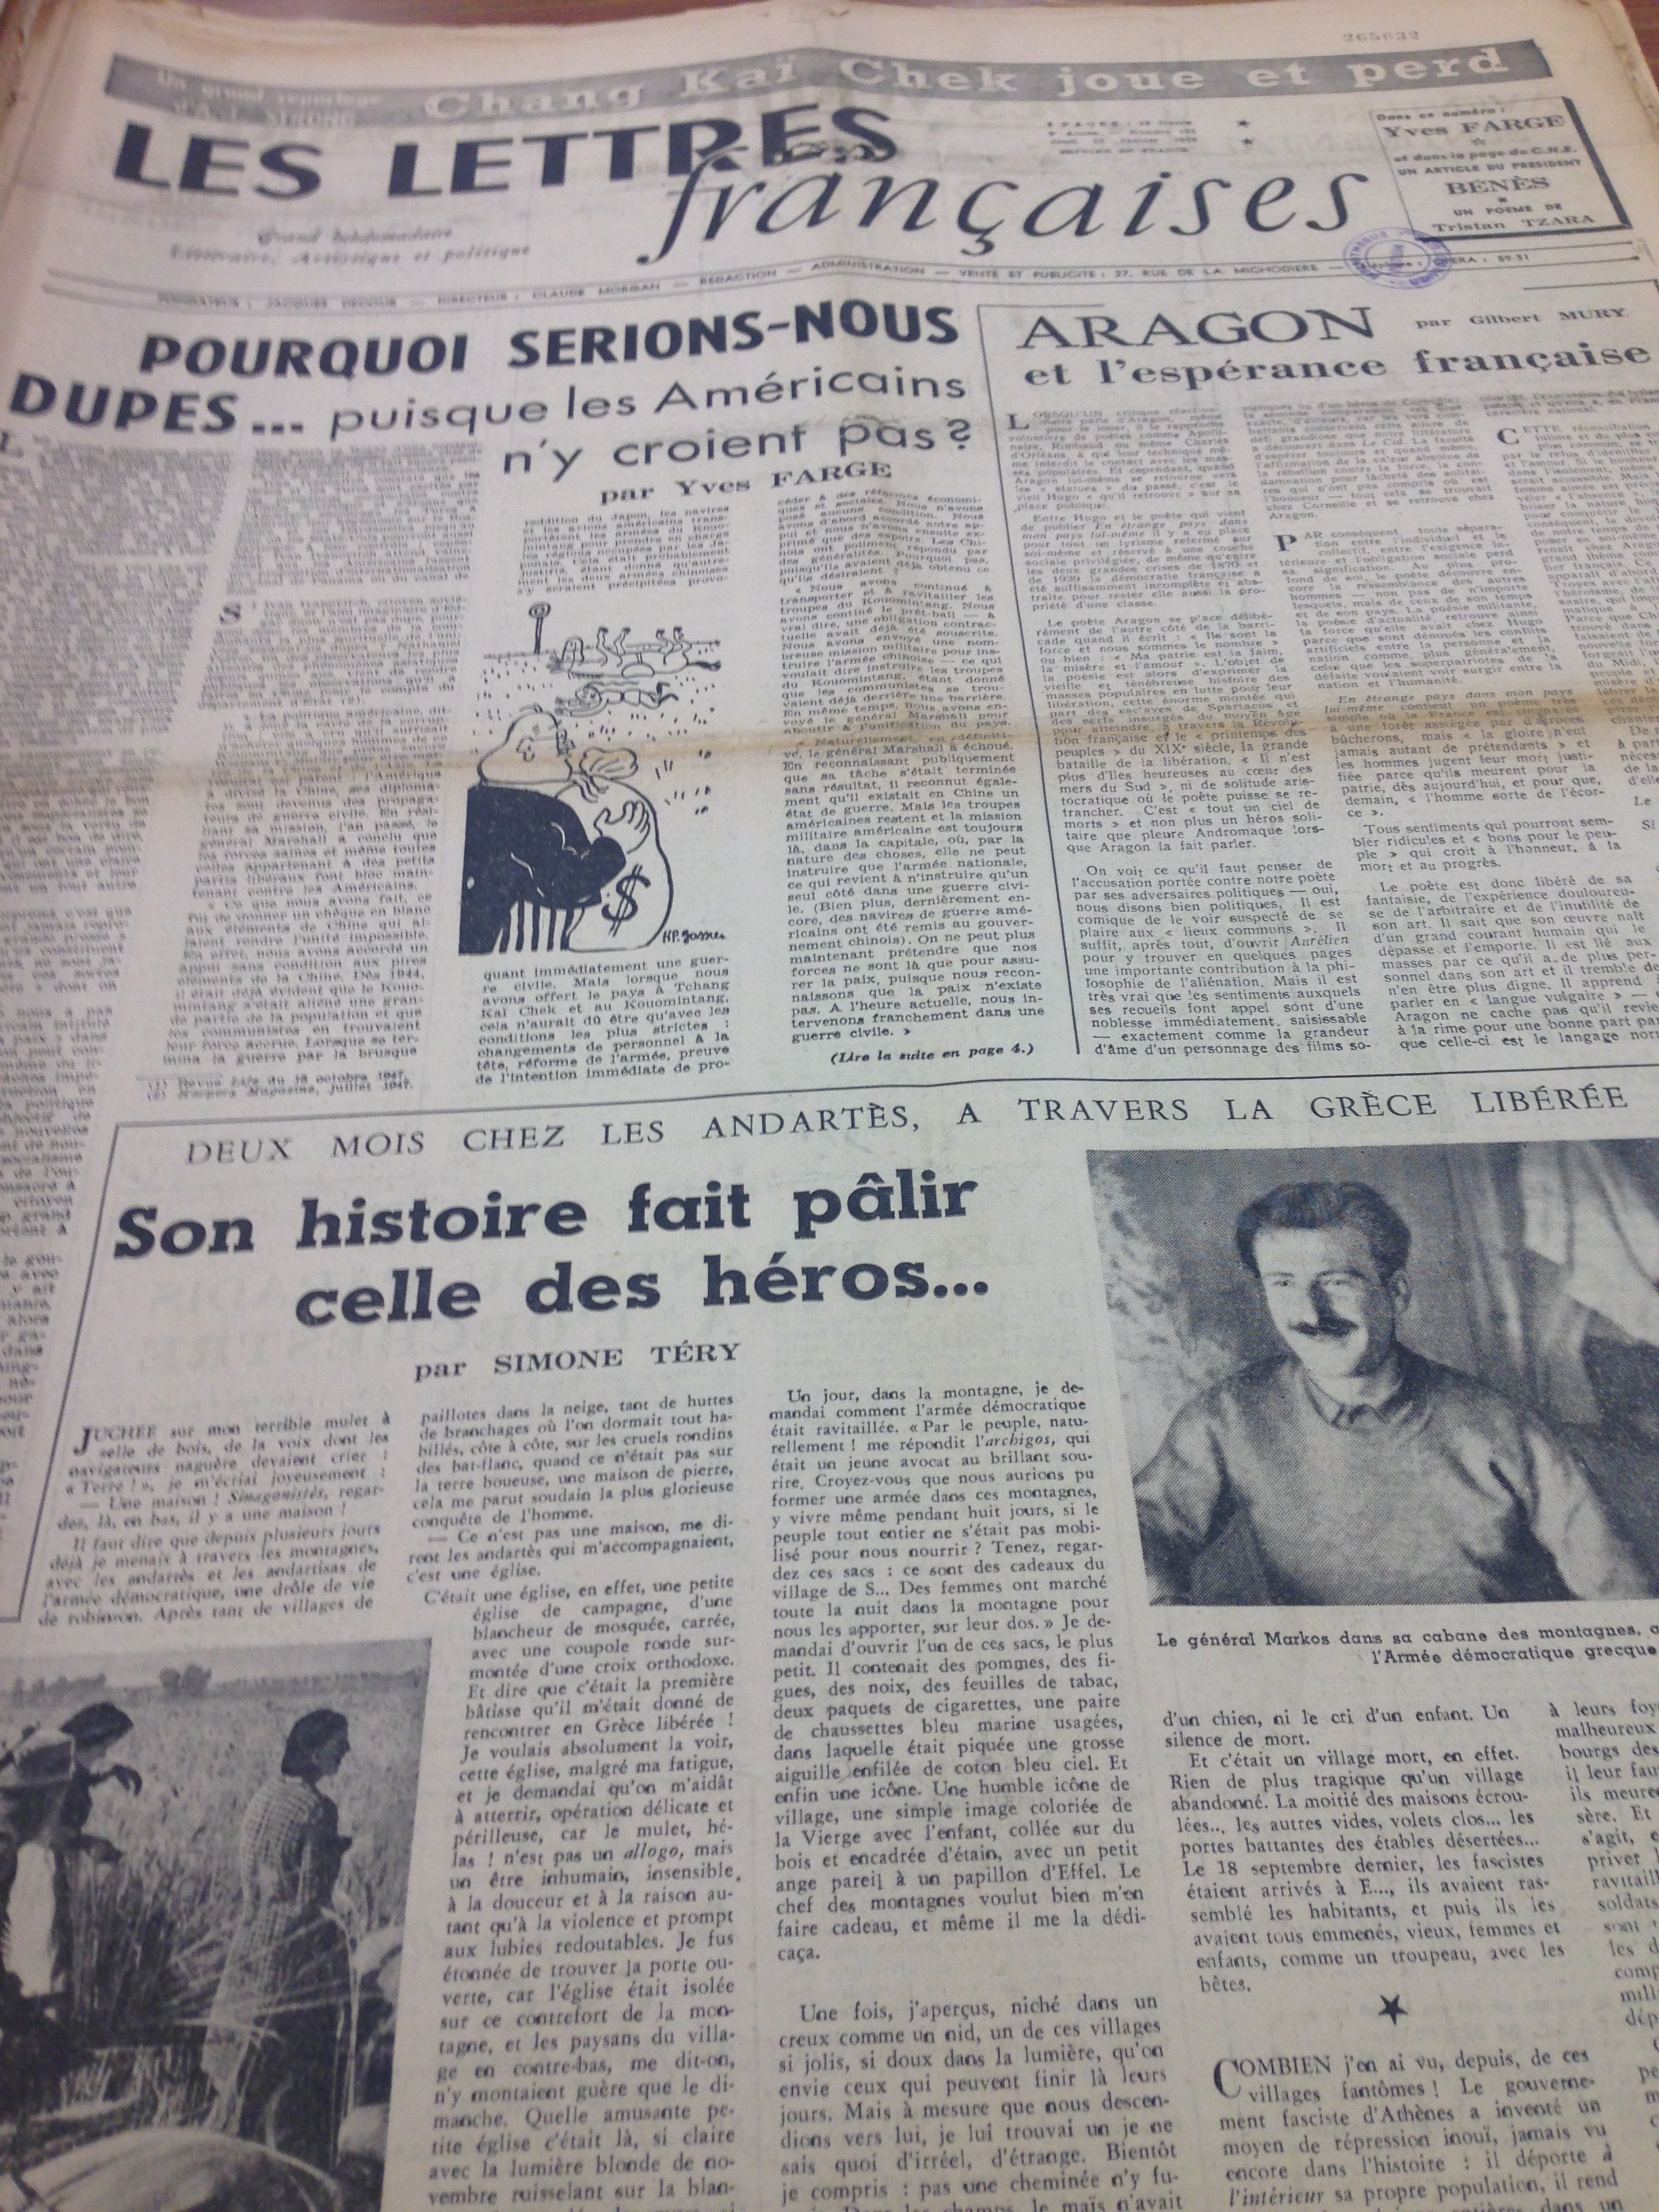
\includegraphics[width=0.33\textwidth]{27janvier1948.jpg}
	\caption{\cite{journallimbour}}\label{fig:}
\end{figure}


	D’une part, Mury emploie la métaphore des barricades, qui dans l’imaginaire collectif rappelle l’épisode de la Commune de Paris. D’autre part, il prête à la Commune un aspect romantique lorsqu’il extrait des fragments des poèmes \emph{Richard Coeur de Lion} et \emph{Plus belle que les larmes}, deux poèmes du recueil \emph{Les yeux d’Elsa}. La figure de la femme aimée se trouve ainsi mêlée à  celle de la patrie. Que le propos politique de l’article ait une portée romantique se confirme d’autant plus avec la seule allusion à une oeuvre romanesque d’Aragon, \emph{Aurélien}. Si Aragon est d’ailleurs désigné dans l’article avant tout comme poète, c’est aussi pour pointer une forme qui reflète le romantisme insurrectionnel : \enquote{Aragon ne cache pas qu’il revient à la rime pour une bonne part parce que celle-ci est le langage normal courant, l’expression du lyrisme populaire et qu’elle a, en France, un caractère national.}

	Toutefois, on ne peut ignorer le double enjeu du message de Mury, qui ne vise pas seulement à louer le lyrisme révolutionnaire, mais aussi à opposer celui-ci contre les Américains, c’est-à-dire par opposition au gros banquier américain caricaturé à côté de son article, lui bien loin de toute forme insurrectionnelle ou poétique avec son gros sac de dollars dans les mains. C’est pourquoi Mury en appelle en partie contre les Américains par la biais du lyrisme patriote. Que les choix de fragments de vers d’Aragon proviennent du recueil d’Aragon écrit pendant la Résistance s’inscrit directement dans la politique éditoriale du journal. 

Cependant, Mury attribue à l’imaginaire romantique d’Aragon son origine au coeur de la lutte des peuples et son apothéose qu’a été la Révolution Française : 

\begin{quote}
 L’objet de la poésie est alors d’exprimer la vieille et ténébreuse histoire des masses populaires en lutte pour leur libération, cette énorme montée qui part des esclaves de Spartacus et des serfs insurgés du moyen âge pour atteindre à travers la Révolution française et le “printemps des peuples“ du XIXème siècle la grande bataille de la libération.   
\end{quote} 

 La synthèse de l’histoire de ces révoltes suit clairement la ligne de peuples en révolte, c’est-à-dire en situation de résistance face à l’oppresseur. On pourrait d’ailleurs substituer à l’\enquote{espérance française} le terme \enquote{résistance} lorsque Mury conclue : 

 L’espérance française apparait ainsi avec ses objectifs bien précis de lutte contre l’envahisseur, et plus largement de défense matérielle et morale du pays. Elle est, comme la poésie d’Aragon elle-même, la forme que revêt la France depuis 1939 et pour longtemps encore l’affirmation exigeante, agressive, quotidienne d’un infini purement humain et inséparable de l’homme.

	 En somme, l’\enquote{espérance française}, c’est la Résistance. Et Aragon, en est à la figure d’autorité par excellence, d’autant plus avec le réalisme socialiste, sa fonction purement patriotique, qu’il incarne par opposition à l’invasion culturelle américaine ressentie par les dirigeants des \emph{Lettres françaises}. 
\subsection{La place d'André Masson dans la politique de la Guerre Froide}

     Quel rôle joue la figure d’André Masson dans \emph{Les Lettres françaises} au moment où la Résistance veut jouer un rôle partisan de la patrie pendant la Guerre Froide ? Un entretien d’André Masson relaté par Claudie Planet\footcite{entretienmasson} est publié en mars 1949. Bien qu’André Masson ne puisse pas directement s’inscrire dans le combat mené par la direction du journal contre la culture américaine, il est intéressant de relever qu’André Masson déclare lui-même être en pleine période d’évolution de perspective de son art. L’article est d’ailleurs accompagné de deux photographies : La première perceptible est l’illustration d’une peinture d’André Masson de 1947, \emph{Portrait de l’artiste par lui-même}. La seconde est une photographie de Masson de dos en train de peindre sur la toile. Il est donc intéressant de relever qu’au moment où le journal \emph{Les Lettres françaises} démarre sa campagne à la gloire de la culture soviétique contre les Américains, André Masson s’établit, après son exil aux Etats-Unis pendant la guerre, en Provence. On imagine quel changement de regard s’opère pour cet exilé de retour en France. Peut-être cet entretien est-il d’ailleurs, sinon la première, l’une des premières collaborations d’André Masson avec le journal.
	 
\begin{figure}[H]
   \centering
   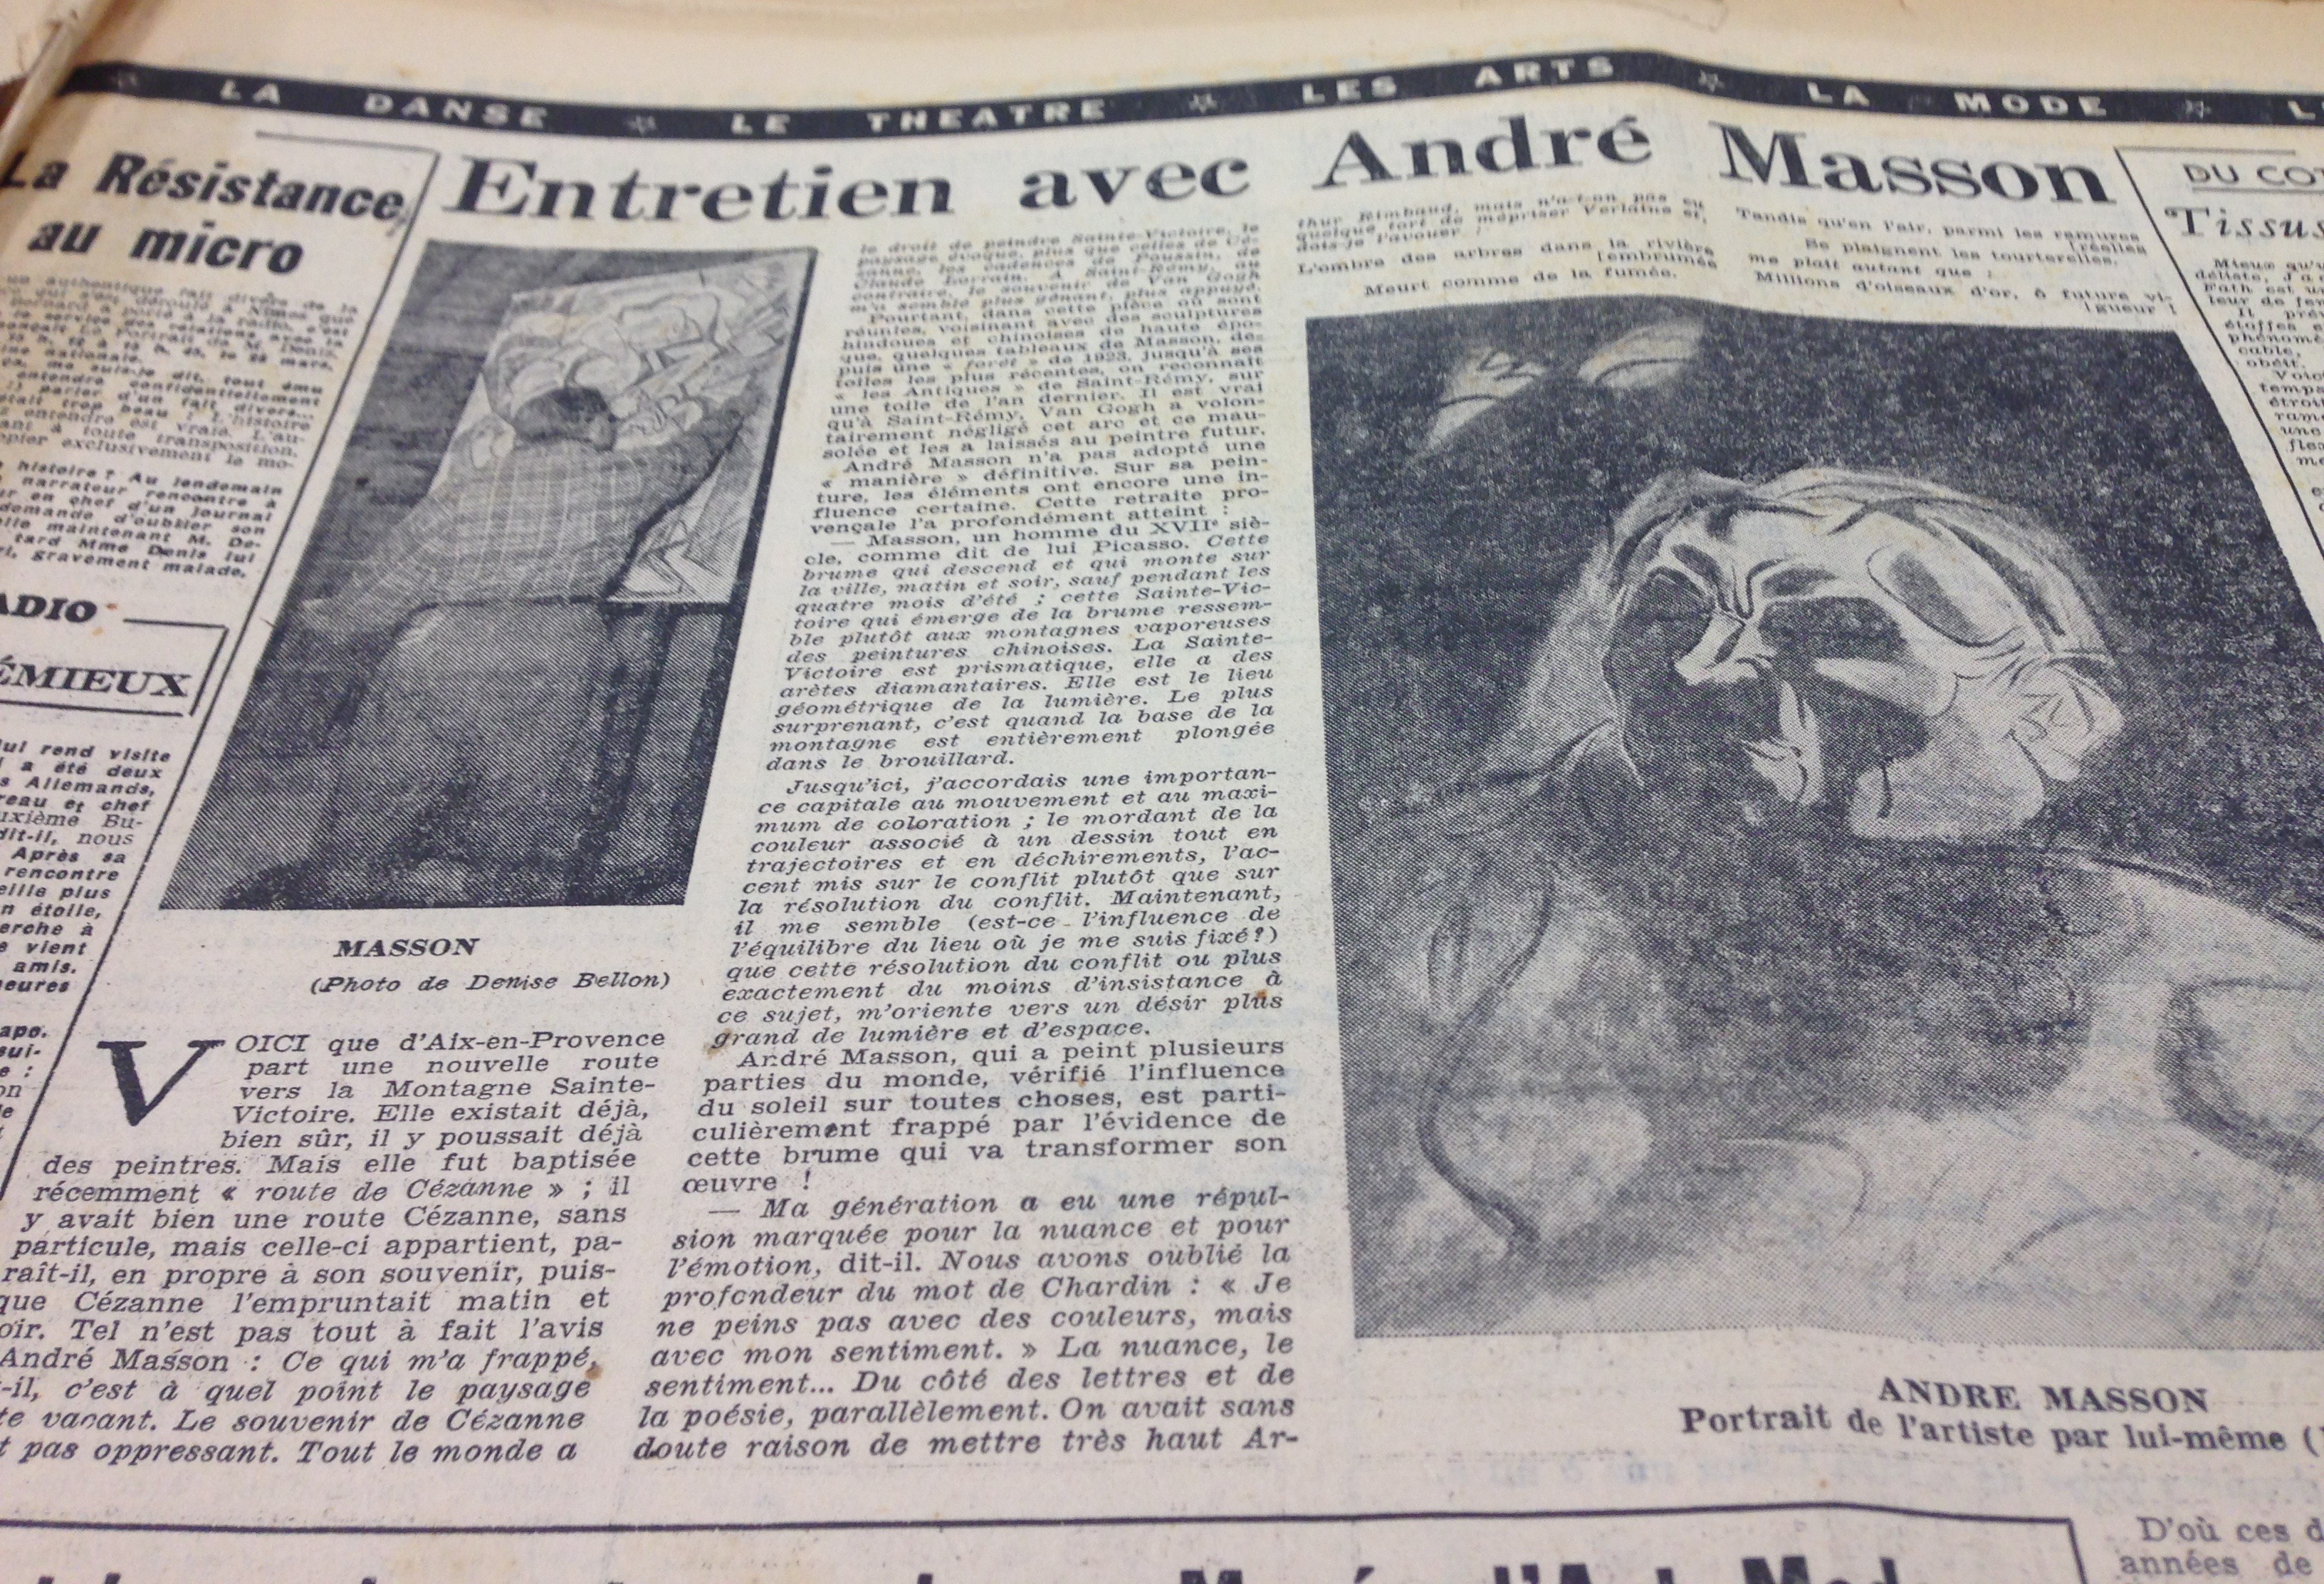
\includegraphics[width=0.33\textwidth]{pageplanet.jpg}
	\caption{\cite{entretienmasson}}\label{fig:Planet}
\end{figure}


Or, force est d’admettre que de ce déplacement de regard le message politique ne peut plus être tout à fait le même : 
\begin{quote}
  Jusqu’ici, j’accordais une importance capitale au mouvement et au maximum de coloration; le mordant de la couleur associé à un dessin tout en trajectoires et en déchirements, l’accent mis sur le conflit plutôt que sur la résolution du conflit. Maintenant, il me semble (est-ce l’influence de l’équilibre du lieu où je me suis fixé ?) que cette résolution du conflit ou plus exactement du moins l’insistance à ce sujet, m’oriente vers un désir plus grand de lumière et d’espace.  
\end{quote}
 

	Non seulement c’est André Masson lui-même qui marque avec ses propres mots une nouvelle étape dans son art, mais il semble distinguer en substance celle-ci, lorsqu’il évoque les \enquote{conflits} de sa série de dessins \emph{Massacres} des années 1930. En réalité, ce n’est pas tant le message politique qui change que le déplacement de perspective. C’est pourquoi, même si André Masson est clairement à rebours du conflit politique qui occupe l’esprit des \emph{Lettres françaises} de cette fin des années 40, lui aussi se plonge dans une période de transition. On peut d’ailleurs relever un brin d’ironie entre le choix de l’autoportrait de Masson choisi pour le présenter par le journal vis-à-vis des nouvelles considérations esthétiques évoquées dans l’entretien : Si Masson concède dans l’entretien posséder « deux faces », la lumière et l’obscurité, et sa préférence en train d’advenir pour la lumière, Claude Planet conclue en précisant \enquote{tout ce que vient de nous dire Masson est confirmé soudain par cette vapeur qui trouble leur netteté et qu’il est impossible de ne pas voir.} Comme si l’attrait de Masson de la lumière résiderait dans cette exploitation du \emph{sfumato}. 


\begin{figure}[H]
   \centering
   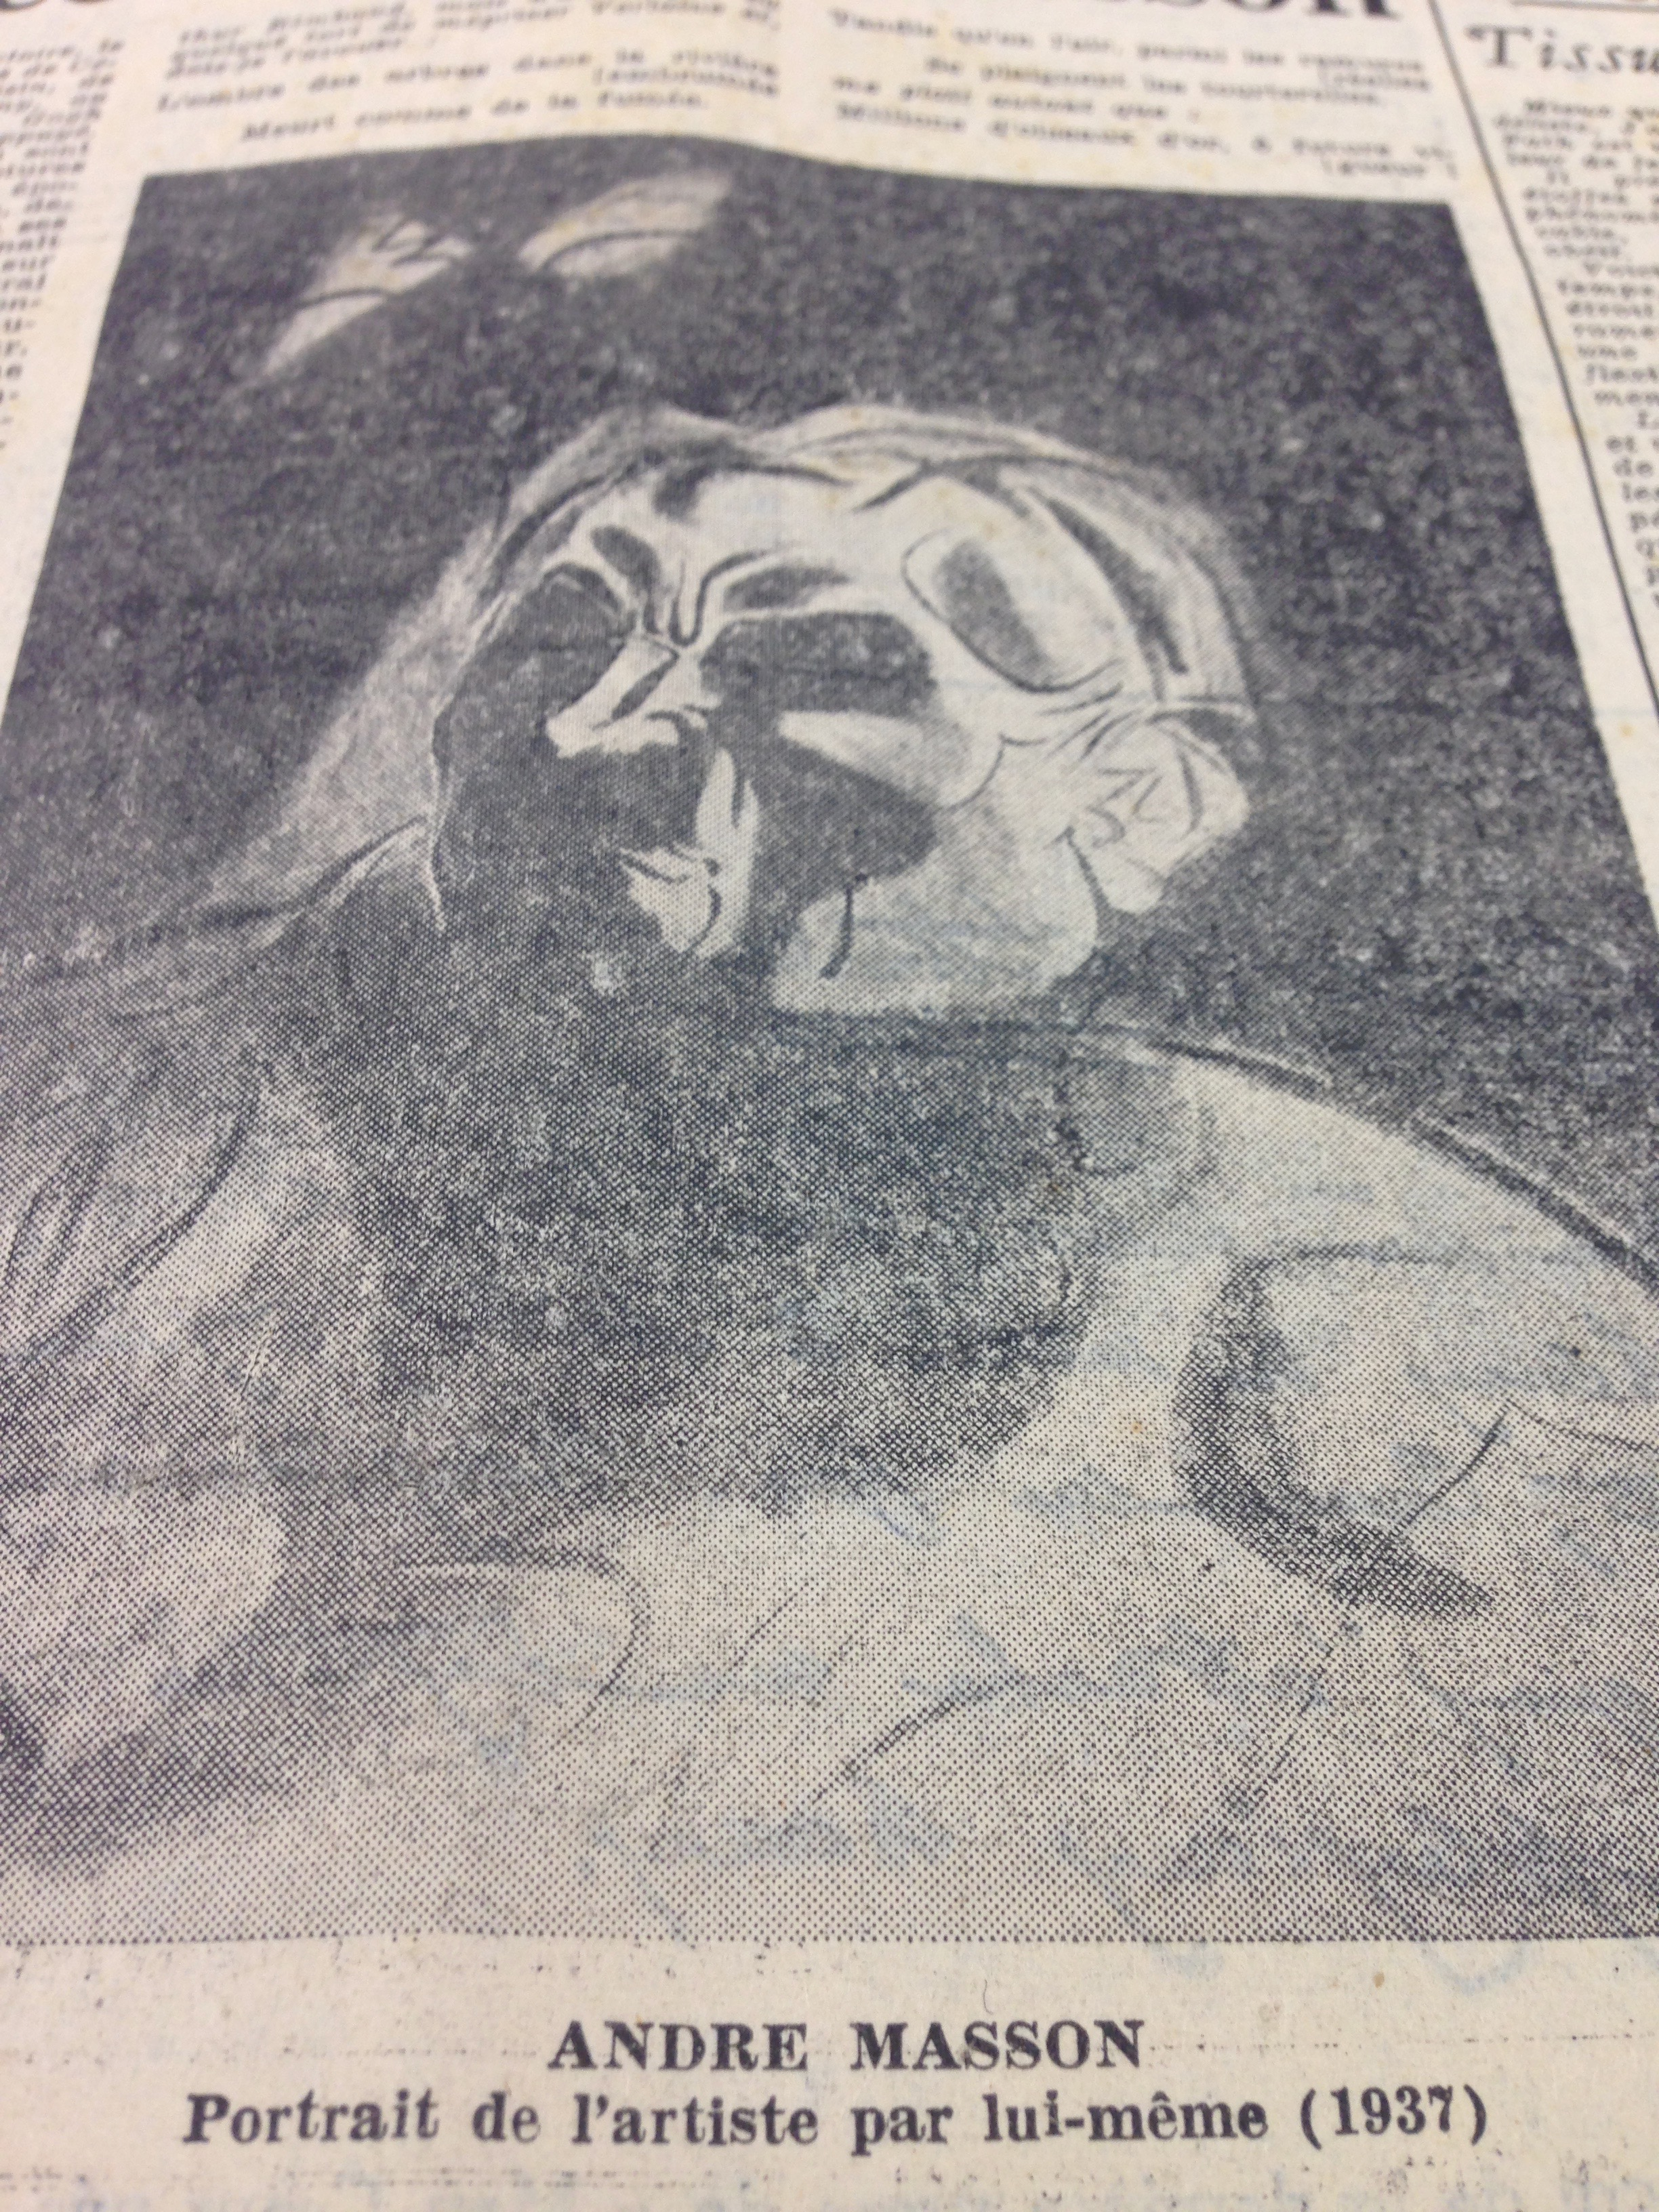
\includegraphics[width=0.33\textwidth]{artistemasson.jpg}
	\caption{\cite{entretienmasson}}\label{fig:Autoportrait}
\end{figure}

\begin{figure}[H]
   \centering
   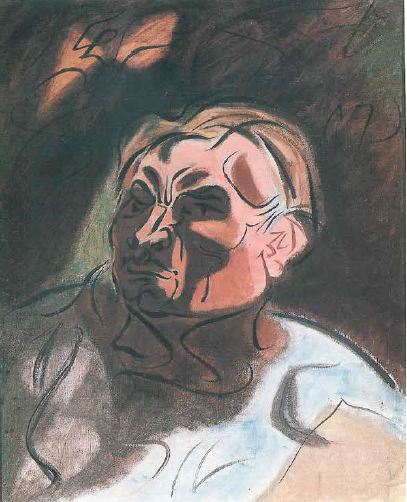
\includegraphics[width=0.33\textwidth]{massoncouleur.png}
	\caption{\cite{entretienmasson}}\label{fig:Autoportraitcouleur}
\end{figure}


Néanmoins, bien que l’autoportrait de Masson soit reproduit en noir, et blanc, les couleurs originelles peuvent interpeller après ce discours de Masson : A l’inverse de l’entretien, le décor est du côté de l’obscur avec un jeu d’ombre à l’arrière-plan avec des teintes de rouge vif similaires à la couleur du visage, plus proche d’un masque que d’un visage humain. Or, c’est la lumière qui transperce ce décor sombre. L’autoportrait de 1947 agit donc exactement à l’inverse des attirances esthétiques que provoque la Provence chez Masson. Mais, si l’obscurité fait surgir la lumière, et la lumière provençale la brume, quel est le véritable élément des deux l’origine du désir du Masson de cette période ? Toujours est-il que, si André Masson ne peut pas participer comme le ferait Fougeron directement dans la bataille des \emph{Lettres françaises }contre la culture américaine, même si lui n’appelle pas directement à la paix, son témoignage sous-entend qu’il recherche ainsi lui cette fois la \enquote{résolution} du conflit. Sans que Masson se confonde dans le parti pris du journal, une proximité intellectuelle se tisse.  

\section{Les enjeux de la politique éditoriale : [n\degre1085- du 17 au 23 juin 1965] et  [n\degre1100- du 7 au 14 octobre 1965] :}

subsection{Les correspondances entre le journal et l'oeuvre romanesque}

Comment la résistance évolue-t-elle au moment des grandes innovations éditoriales ? Quel rôle joue la résistance nourrie par la réflexion des mediums qu’à la direction des \emph{Lettres françaises} en 1965 sur son propre journal ? Deux ans avant \emph{Blanche ou l’oubli}, la direction en annonçant en première page les raisons du prochain format et organisation des numéros à venir à la rentrée de l’automne, l’aspect médiatique est au coeur de la question du changement adapté aux considérations idéologiques du journal :

\begin{quote}
Aussi important est l’essor de la télévision et ses perspectives immédiates, par exemple. Mais l’expansion des sciences, de toutes les sciences humaines, comme de la nature, le progrès prodigieux des techniques, font que la véritable source de multiplication se trouve dans les transformations inégalées tant en ampleur qu’en rapidité de notre vie, de nos conceptions, de notre psychologie. Un journal comme le nôtre n’a de sens que s’il est capable de refléter ces changements.\footcite{nouvelleformule}\end{quote}


	Tout un pan de la politique éditoriale cherche à s’ancrer dans les évolutions de la société, en particulier technologiques, mais aussi pour les conséquences réceptives, émotives, qui en résultent.

\begin{figure}[H]
   \centering
   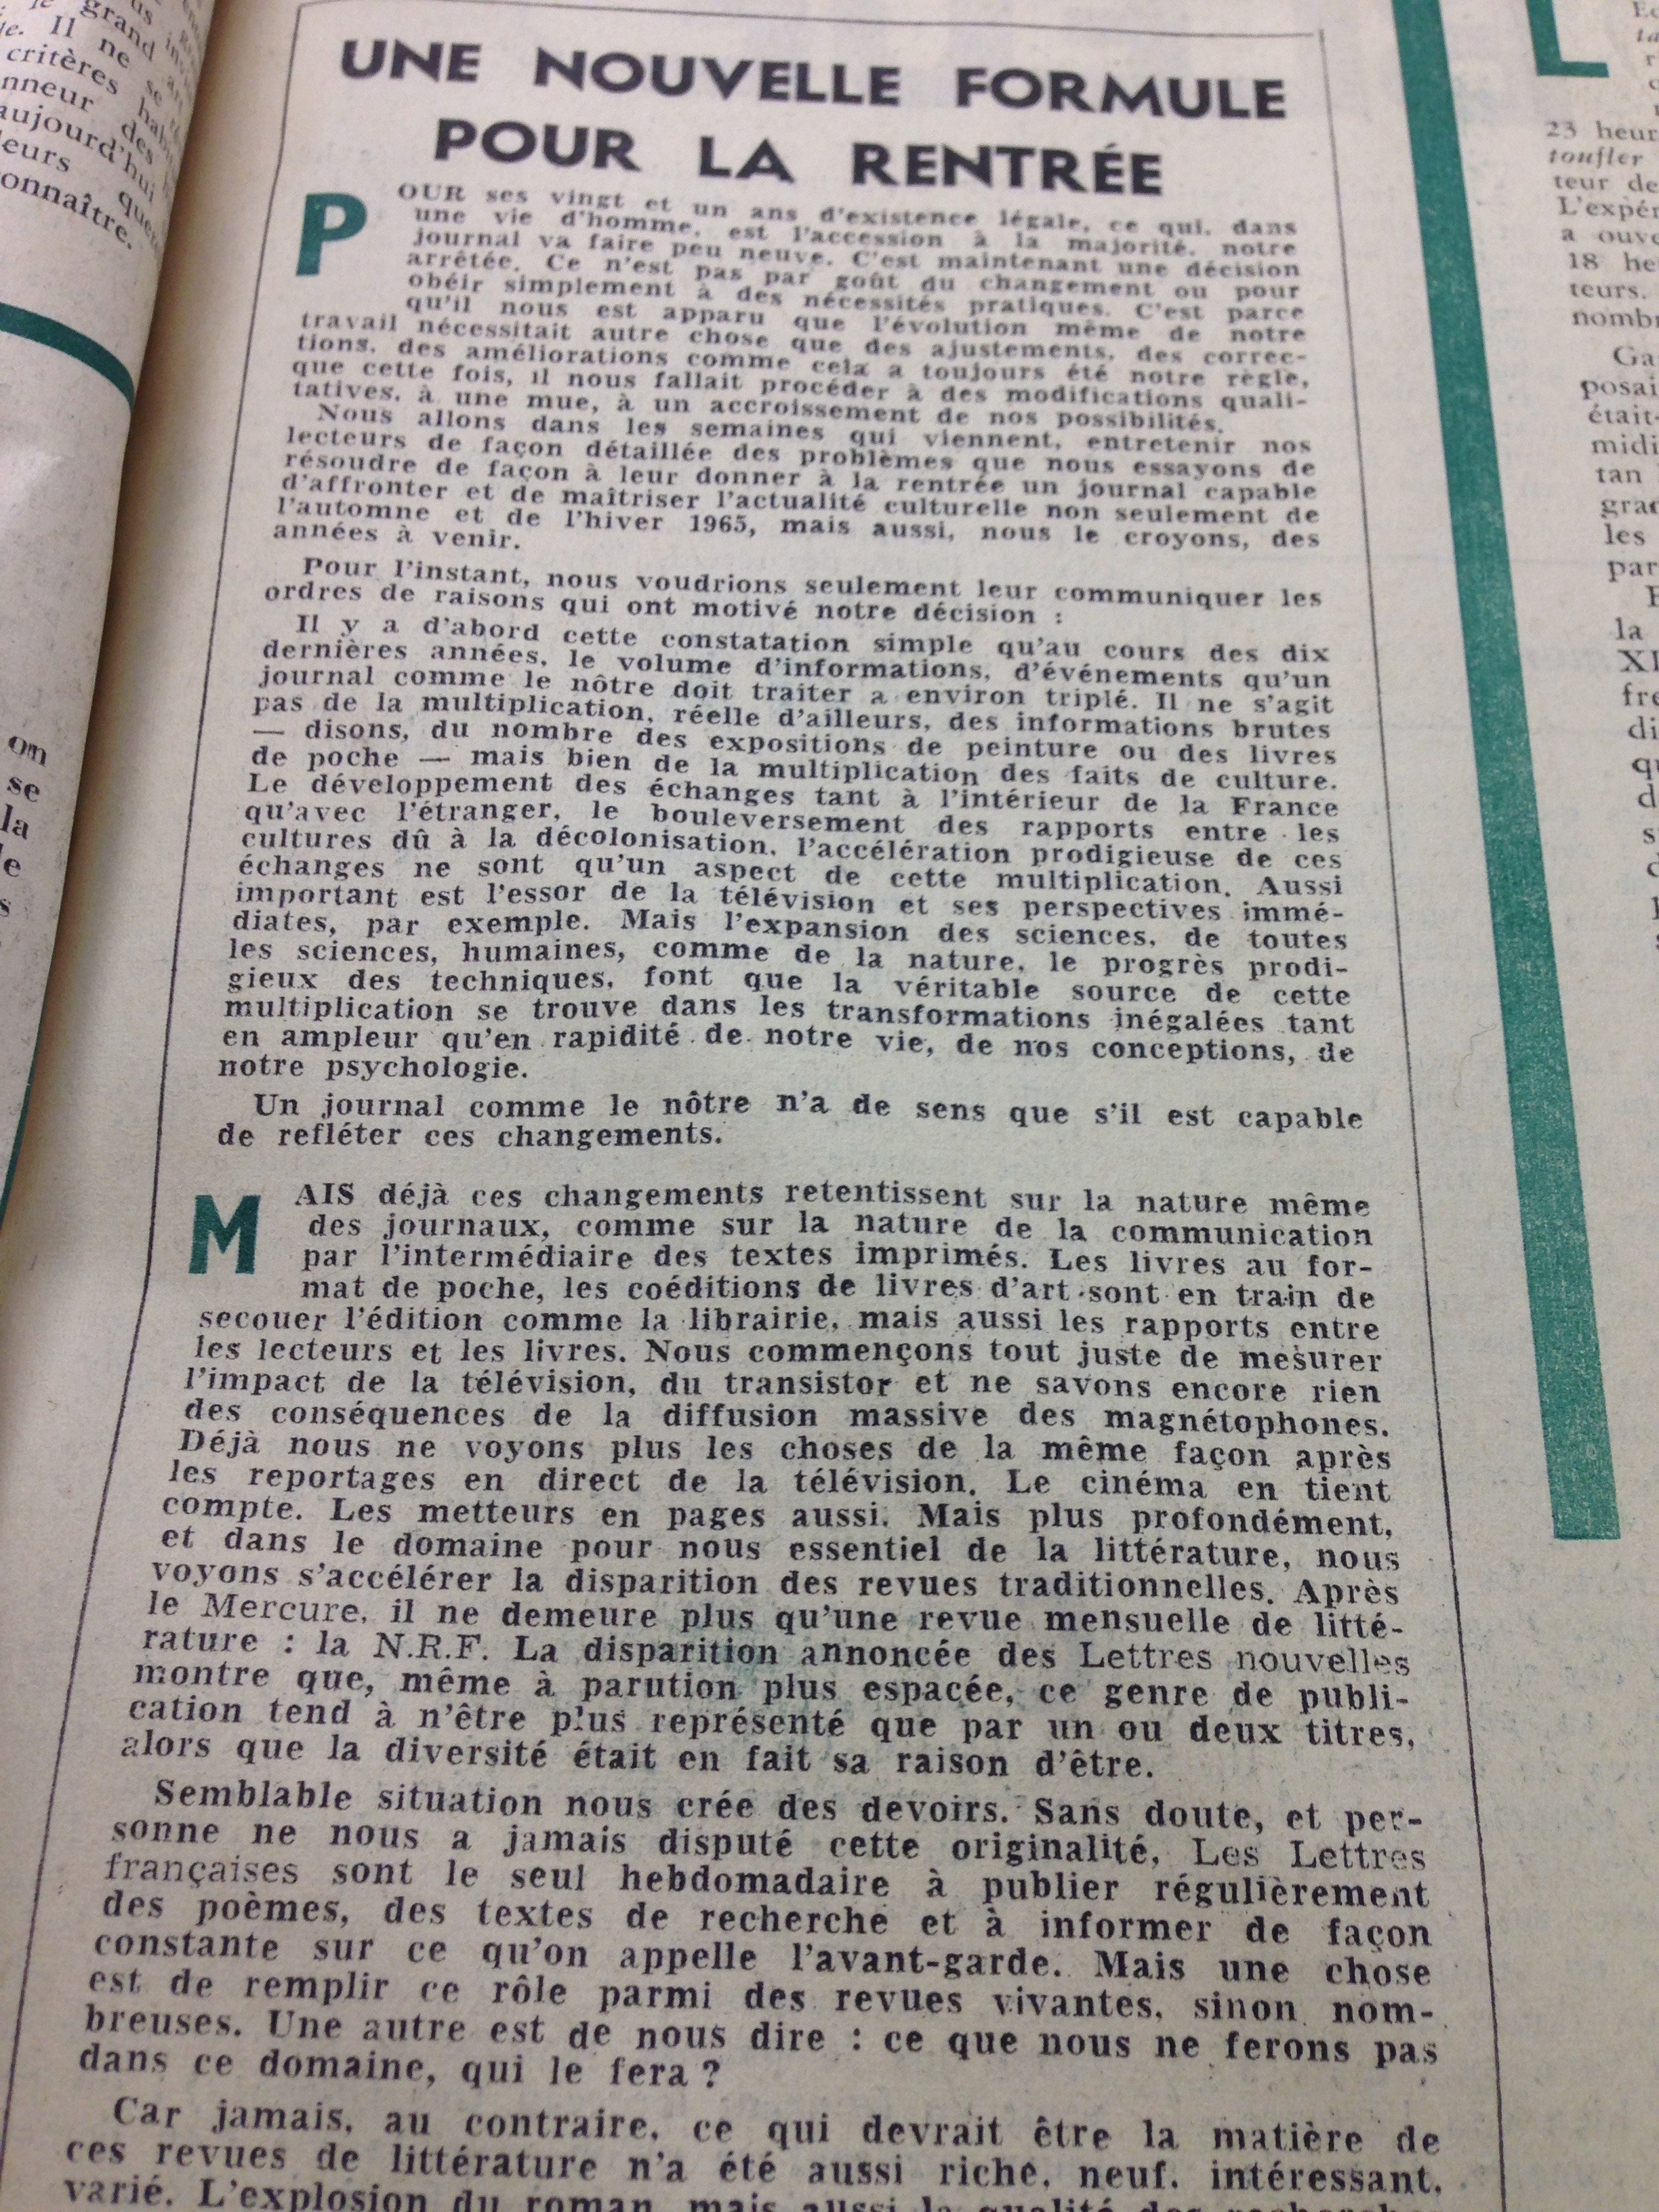
\includegraphics[width=0.33\textwidth]{nouvelleformuleannonce.jpg}
	\caption{\cite{nouvelleformule}}\label{fig:annoncenvformule}
\end{figure}


	C’est pourquoi en même temps que l’aspect de la politique éditoriale des \emph{Lettres françaises}, on pourrait facilement croiser la réflexion pour la prochaine formule des numéros à venir et celles romanesque de \emph{Blanche ou l’oubli}. Ouvrage de 1967 mais dont l’action a lieu en 1965. Le point commun essentiel réside dans le constat d’Aragon des évolutions technologiques et de la révolution dans ce domaine que cette période est en train de vivre, et paradoxalement ce que produit cette intelligence collective comme lien intime sur l’homme en tant qu’individu. La résistance au sens d’Aragon comme directeur des \emph{tLettres françaises} en 1965, c’est encore une fois un processus qui prend en compte l’étape de transformation qu’est la révolution, mais sous diverses formes, y compris celle de transformer le journal en fonction des changements de perceptions sur les individus que sont en train de produire les développements technologiques sur les individus.

	 En outre, la Résistance est directement déplacée dans \emph{Blanche ou l’oubli} dans la perspective des nouvelles technologies et de la réception qu’elles provoquent : \enquote{“- Oh ! - il fait, Philippe -, tu la ramènes, avec la Résistance. Cette année, c’est bien simple, la télé n’était pas visible !“}. La tonalité humoristique n’exclue en rien la prise en compte par Aragon de cette génération venue après lui qui n’a pas vécu cette période historique. C’est donc aussi la jeunesse qui est interpellée dans la réflexion d’une nouvelle formule du journal, celle à qui Aragon entend parler en tant qu’auteur et directeur de journal. 

	Cette idée rejoint l’autre grand mot d’ordre propre plus à Aragon probablement qu’à son prédécesseur Claude Morgan, qui serait de joindre le passé de résistance à la pluralité. A ce titre, Aragon voit en son lecteur également un spectateur, d’où la prolifération d’images et pas seulement dans les rubriques d’Art, mais aussi comme individu dans l’ère de son temps. Si cette réflexion sur l’évolution technologique rencontre la fameuse question des Livres de poche, cette pensée de la direction rappelle une fois encore la pensée du prochain roman d’Aragon, riche des grandes enquêtes de 1964 entreprises par \emph{Les Lettres françaises} sur le livre de poche : \enquote{Marie Noire oublie la comète, oublie sur un guéridon son \emph{Livre de poche}, elle se lève et se voit, s’imagine dans le miroir au-dessus de la cheminée} , ou encore :
	\begin{quote}
	 Marie Noire n’a pas lu la Correspondance, on n’en est pas encore à en faire des romans d’espionnage, je veux dire des Livres de poche. Elle se regarde dans la glace, et elle y voit au fond, tout nu, assis sur ses jambes, ce garçon qui lui a dit je t’aime.\footcite[p102]{blancheouloubli}\end{quote}

	  On ne peut ignorer que ces deux références à la même page au livre de poche précèdent directement une autre référence-clé chez Aragon, particulièrement visible en cette année de 1965 avec \emph{La mise à mort}, le miroir. L’intelligence des machines d’une part, celle du livre de poche d’autre part, comme reflet de l’homme. 


Mais l’échange entre ces numéros et le roman à venir ne s’arrête pas-là. Cette réflexion au coeur de \emph{Blanche ou l’oubli} existe non seulement comme enjeu de politique éditoriale dans la nouvelle formule de 1965, mais les numéros qui font allusion à cette fameuse nouvelle formule du journal \emph{Les Lettres françaises} existe eux-aussi comme allusions dans \emph{Blanche ou l’oubli} : \enquote{Ce n’est pas très important, et il est vrai que ce roman n’a été inclus dans le Livre de poche qu’au mois de juin 1965. Pas cinq mois. ça suffit pour qu’en octobre…}. En faisant allusion à la parution de \emph{L’Education sentimentale} en livre de poche, le narrateur mentionne le mois de « juin 1965 », qui est celui où \emph{Les Lettres françaises} annonce en première page réfléchir à une nouvelle formule du journal à compter de la rentrée d’octobre. Et c’est justement dans le numéro du 7 octobre 65 que parait la fameuse nouvelle formule. Peut-on voir ainsi dans cette rêverie autour du Livre de Poche un clin d’oeil à ces deux numéros précisément qui en plus le livre de poche comme modèle d’une nouvelle formule du journal publient dans le numéro suivant la suite de l’article \emph{Une nouvelle formule pour la rentrée (II), La révolution du livre }? Quoi qu’il en soit, la politique éditoriale du journal, à partir de son mot d’ordre de résistance, dérive par de multiples axes jusqu’à réapparaître et retrouver leurs réflexions poursuivies dans les oeuvres romanesques même d’Aragon. Un jeu de correspondance s’établit donc entre le journal et les romans, ainsi qu’un autre niveau de lecture où le roman fait allusion aux articles des \emph{Lettres françaises}. 


\subsection{Masson comme médiateur entre Elsa et la Résistance}

En comparaison, le rapport d’André Masson à la Résistance n’est pas similaire à celui d’Aragon. Ce dernier, en tant que poète et  directeur du journal, dans un numéro de  1965,  revenait encore  sur la naissance du journal \emph{Les Lettres françaises} et du CNE\footcite{histoirecnetriolet}, l’autre grande création pendant la Résistance\footcite{specialelsa} dans laquelle Aragon et Elsa Triolet jouent un rôle de premier plan. Néanmoins, un numéro de 1971 très particulier exploite le ressenti d’André Masson face à la Résistance : Il s’agit d’un numéro spécial en hommage à la mémoire Elsa. Mais, au-dessus-de la banderole verte des \emph{Lettres françaises}, un autre sujet cohabite avec cet hommage, \emph{Comment écrire l’histoire de la Commune en 1971 ? - Entretien avec Jean Bruhat, Max Gallo, Jacques Rougerie et Georges Soria}. Or, ces deux sujets apparemment distincts sont illustrés la page 2 qui présente le sommaire et des encadrements d’expositions, par la photographie en noir et blanc de la peinture d’André Masson, \emph{Résistance}, de 1944. Dès lors, il s’agit de comprendre non seulement selon quelle logique l’anniversaire de la Commune de Paris, toujours très célébrée par le journal et particulièrement en cette année centenaire, rejoint l’autre grande date pour Aragon qui est l’hommage à Elsa Triolet, décédée le 16 juin 1970. Dans un second temps, la position médiatrice du tableau Résistance en page deux de présentation du numéro laisse sous-entendre que le tableau constitue la ligne directrice commune tant à l’anniversaire de la Commune de Paris qu’à l’hommage à Elsa Triolet. 


\begin{figure}[H]
   \centering
   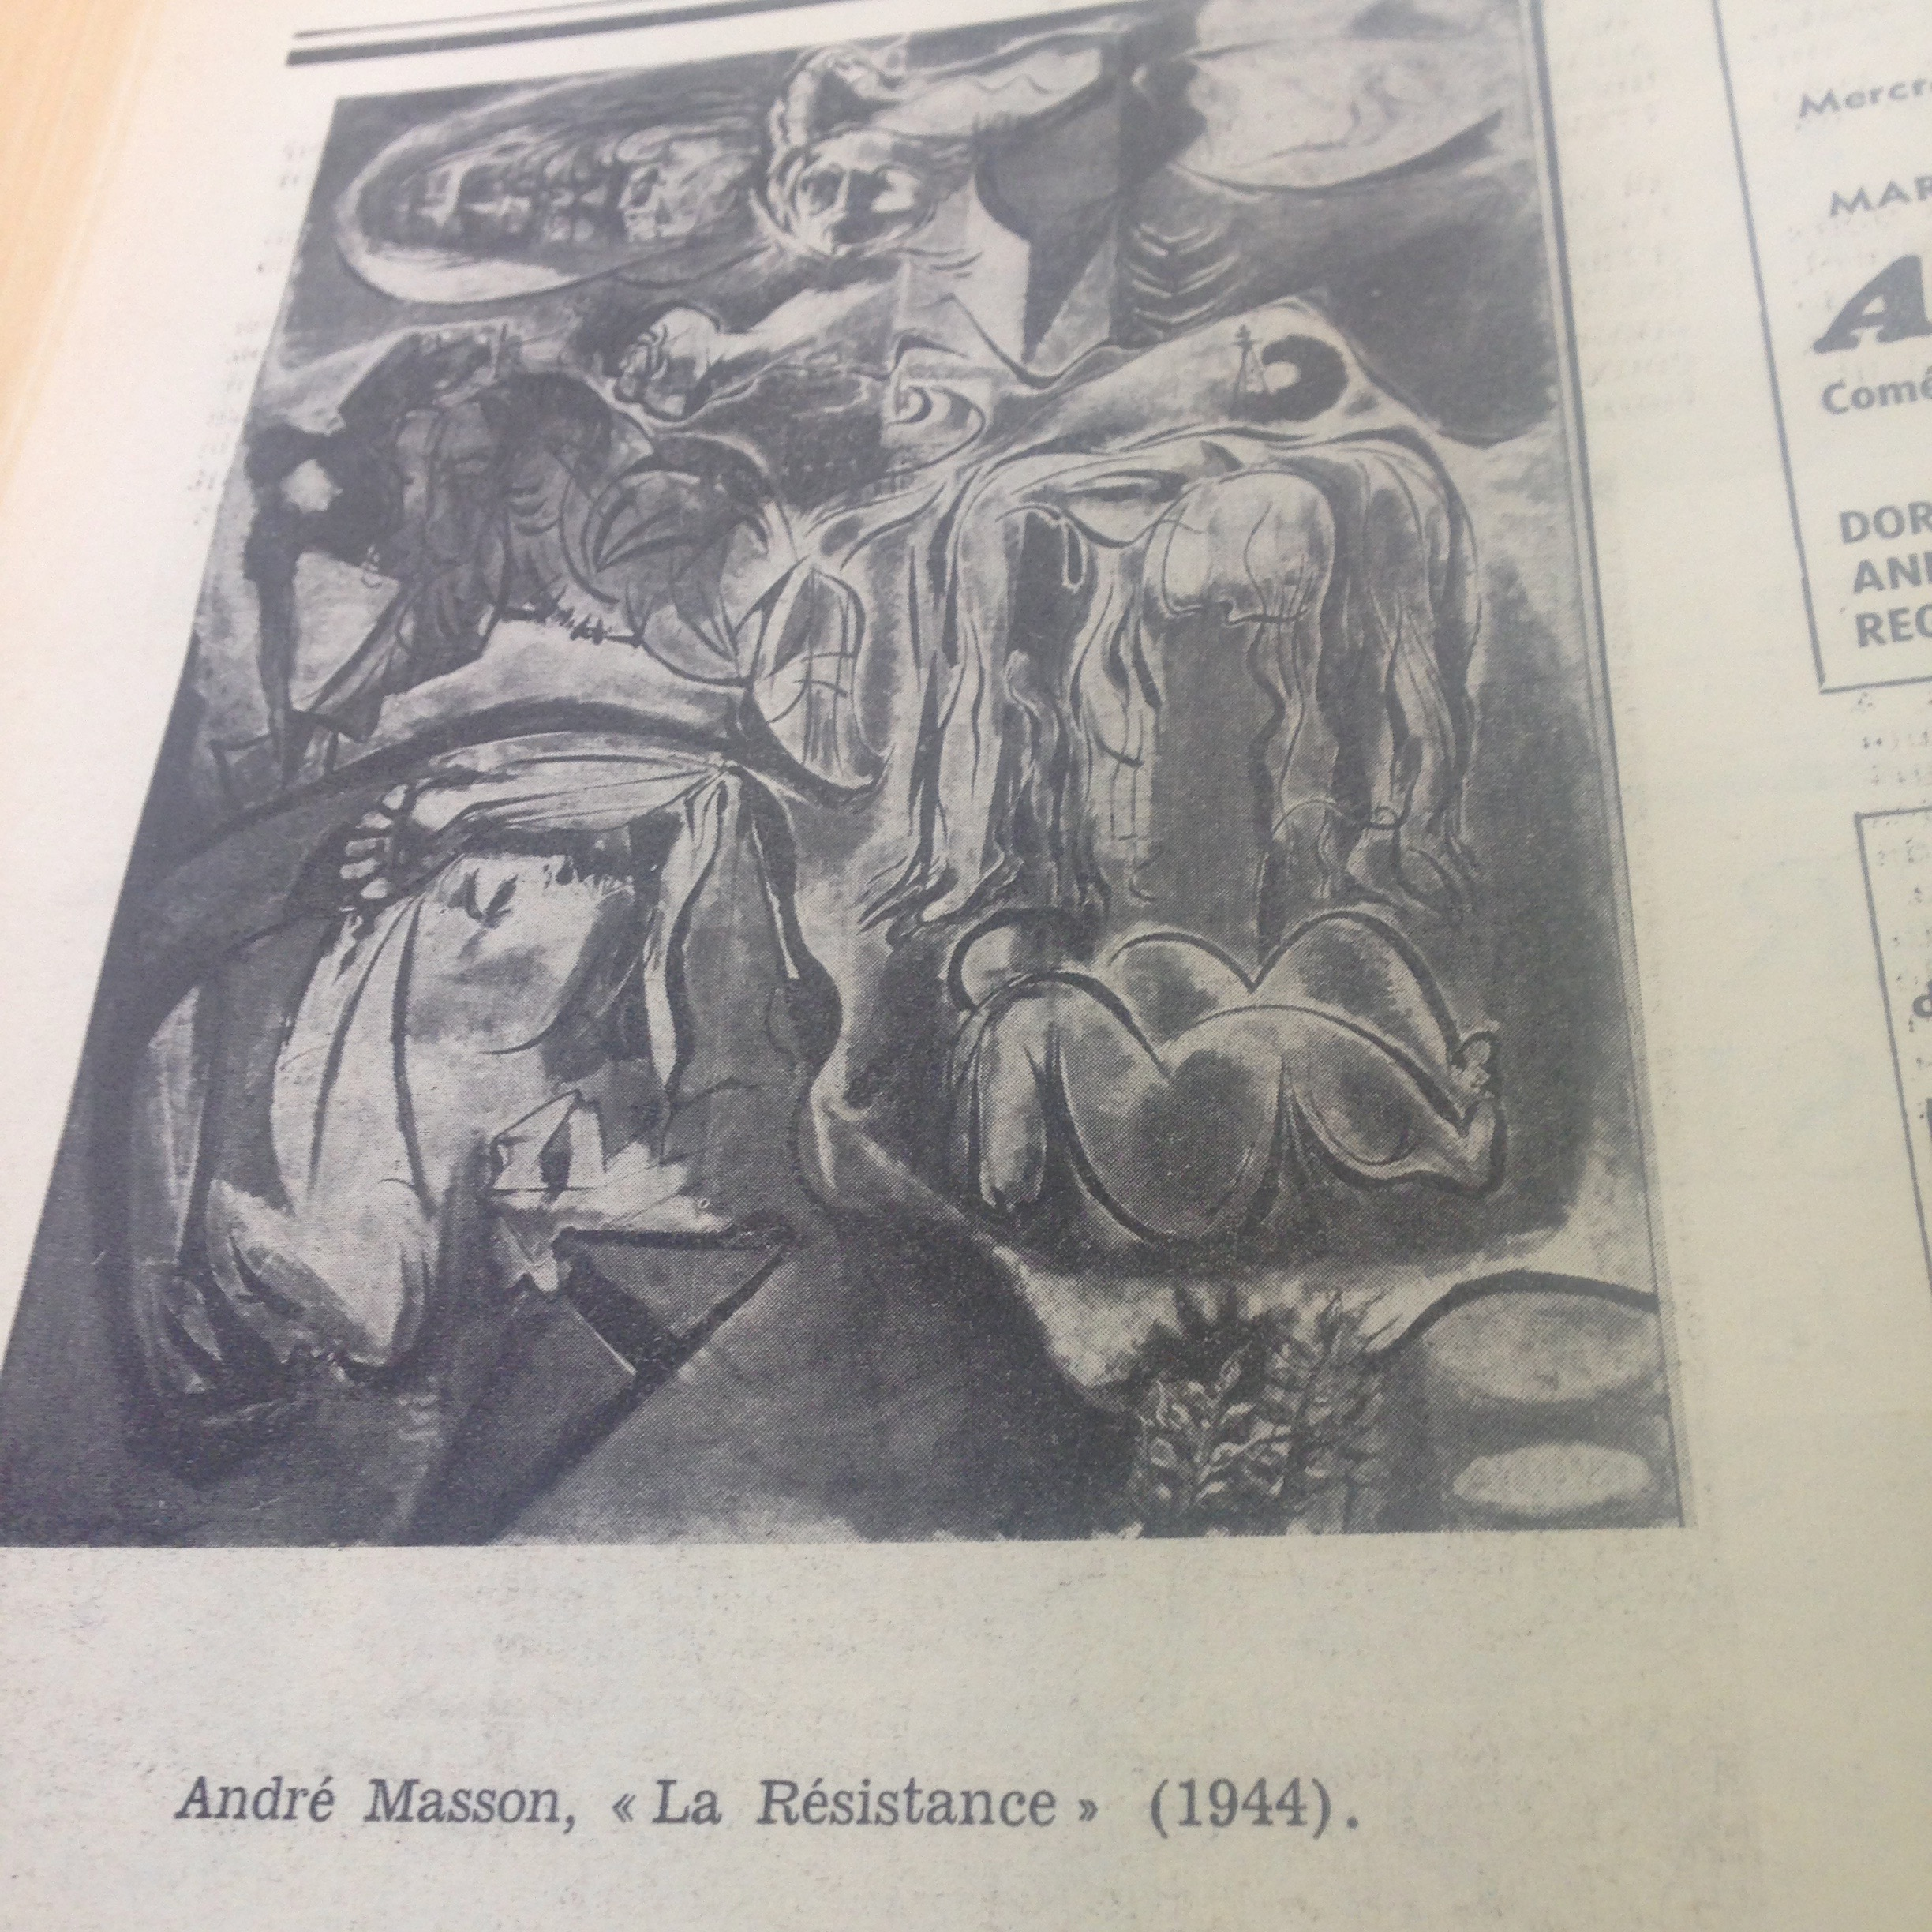
\includegraphics[width=0.33\textwidth]{resistancep2.jpg}
	\caption{\cite{specialelsa}}\label{fig:Resistance}
\end{figure}

\begin{figure}[H]
   \centering
   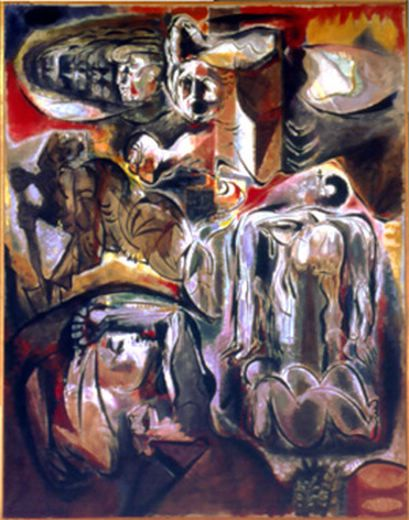
\includegraphics[width=0.33\textwidth]{resistancecouleur.jpg}
	\caption{\cite{specialelsa}}\label{fig:Resistancecouleur}
\end{figure}


C’est d’ailleurs à une troisième période historique auquel renvoie ce tableau de Masson, bien que le sujet ne serait pas immédiatement identifiable sans le titre et la date qui ne laisse pas le doute possible. La figuration n’est d’ailleurs pas plus immédiatement reconnaissable, et il faut s’attarder sur le tableau pour que se devinent derrière les formes apparemment géométriques et flasques le contour de fragments de corps de femme (bas de la toile) et de l’homme barbu qui lui est symétriquement opposé. En fait, on pourrait même se demander si le tableau ne se lit pas plutôt en format paysage. Quoi qu’il en soit, même avec la clarté du titre, le tableau demeure obscur, plus proche de l’énigme à déchiffrer. En outre, en reproduisant le tableau en noir et blanc, en sachant qu’il est arrivé en particulier dans ces années-là au journal de faire des reproductions en couleur, on peut supposer que l’enjeu n’est pas seulement financier mais stratégique : Si on retire les couleurs vives de ce tableau qui imprègnent directement l’attention, l’observateur revient comme souvent sur les formes. Un tel choix se justifie d’autant plus avec le recours au nombreux dessins et surtout esquisses pour les oeuvres d’André Masson en particulier. Sans compter qu’André Masson lui-même est une figure médiatrice particulièrement indiquée pour associer la Commune de Paris de 1871 et Elsa Triolet. D’une part, nous avons eu l’occasion d’analyser l’article \emph{André Masson et la Commune}\footcite{commune} par  Raoul-Jean Moulin avec le témoignage intime et des esquisses du peintre. D’autre part, André Masson avait été l’un des participants à la mémoire d’Elsa Triolet dans le fameux numéro après sa mort en Juin 70, intitulé \emph{Elsa}\footcite{specialelsa}. Son hommage était assez atypique, même vis-à-vis des autres peintres, puisqu’il avait choisi de ne pas écrire de texte pour lui dédier l’un de ses plus fameux  tableaux sur la femme, \emph{Mélusine}. Comprendre la démarche éditoriale et la fonction symbolique qu’y incarne le tableau Résistance de Masson, c’est donc d’abord avoir en mémoire cet autre numéro au moment de la mort d’Elsa, publié dans les plus vives émotions de la perte.


C’est pourquoi, paradoxalement au sujet du tableau, André Masson opère nécessairement d’abord le lien entre deux imaginaires proprement romantiques chez Aragon, la Commune de Paris et la figure d’Elsa. Il n’est pas anodin que, plus que pour aucun autre événement historique, les numéros des \emph{Lettres françaises} constituent une abondante réserve historique de documents sur ce moment de l’Histoire en particulier. Pas plus que prolonger après une première partie sur l’\emph{Après-dire} d’Aragon pour les \emph{ORC} de \emph{Blanche ou l’oubli} où Aragon y exprime l’égarement après la perte d’Elsa, la seconde partie du numéro porte sur l’Histoire de la Commune. Il apparait ainsi que la stratégie éditoriale du journal dirigé par Aragon n’est pas uniquement d’ordre politique et idéologique, comme on a pu le voir dans des exemples précédents, mais aussi d’ordre purement intime. 


	Pourtant, c’est avant tout l’aspect de la rigueur historique qui prédomine dans ce rassemblement d’études d’auteurs sur la Commune. Pas forcément à l’avantage de celle-ci, si l’on pense à l’ouvrage de Jacques Rougerie,\emph{Procès des communards}, plus proche de la désillusion. Si l’image de Louise Michel reste brave, le livre montre aussi qu’elle est plus une exception qu’un exemple, et l’on assiste aux revirements d’opinions de nombreux communards au moment du jugement. Si la Commune est vécue par \emph{Les Lettres françaises} avec une passion sans bornes, depuis 51, à travers la figure de Courbet, ce n’est pas tant par l’idéalisation de la figure romantique du communard révolutionnaire, mais par une démarche plutôt scientifique qui trahit l’obsession du journal pour cet événement historique en particulier : \enquote{Jamais peut-être encore n’a-t-on tant publié de livres pour un anniversaire} introduit la direction en guise de préface à l’entretien, ce à quoi Pierre Daix pose une problématique claire autour de ces quatre ouvrages : \enquote{Comment écrire l’histoire de la Commune en 1971 ?} Or, ce qui ressort le plus précisément de l’entretien animé par Pierre Daix, c’est le point commun de ces quatre auteurs et historiens à aborder les sources sur la Commune non du point de vue de ses grands représentants, mais plutôt du peuple. Et le dessein de ce projet, Jean Bruhat le souligne, et l’on comprend combien il s’imbrique dans la politique culturelle du journal : \enquote{il y aurait beaucoup à rechercher à propos du retentissement de la Commune sur les mentalités ouvrières.}
	Plus qu’aucune autre période historique, le journal a recueilli tellement de documents d’archives sur la Commune que Les Lettres Françaises peut se considérer sur l’ensemble des numéros depuis 51 comme une anthologie de l’Histoire de la Commune de Paris. On peut même y ajouter à cela un autre sujet apparemment distinct et dont pourtant son aspect romantique vient du souvenir de la Commune : Lorsqu’un numéro publie des photos du quartier de Belleville, le souvenir de la Commune n’est pas étranger à cette nostalgie pour ce quartier du XXème. Tout particulièrement dans les années 70 où les numéros déplorent l’architecture de Paris en train de se modifier, perdre une âme d’origine. L’immense article reproduit d’ailleurs un plan de la ville de Paris avant les travaux d’Haussmann. Or, c’est justement la question de l’héritage de la pensée communarde qui réunit les quatre historiens : Son héritage sur les ouvriers d’aujourd’hui d’une part, celle qu’en fit sa digne héritière la révolution de 1917 d’autre part. 


André Masson, le médiateur du numéro, est également mentionné dans la légende du livre de Georges Soria, \emph{La grande histoire de la Commune}, dont l’un des dessins illustre ce grand entretien. Sa position aux côtés du sommaire prête ainsi un autre sens à la période bien précise de la Résistance sous la Seconde Guerre Mondiale. Résistance devient par cette place de choix de présentation du numéro comme la résistance des \enquote{communeux}, qui défendent les barricades de la ville de Paris conte l’armée versaillaise pendant 73 jours. C’est peut-être aussi ce qui explique le choix de la direction des \emph{tLettres françaises} de choisir le tableau de Masson plutôt qu’une photographie de la Commune ou un peintre à l’esthétique plus mimétique : L’énigme qui ressort de cette toile n’évoque pas tant une période historique que la recherche du sens le plus absolu possible du terme \enquote{résistance}. On discerne d’ailleurs difficilement des visages, hormis celui de la jeune femme du bas de la toile, levant un poing musclé plutôt masculin. Elle est opposée symétriquement à l’homme barbu du haut de la toile, dans une attitude plus pensive. Dans ce méli-mélo de fragments de corps, la résistance est avant tout la propre révolte du peintre. Car c’est peut-être là une conception commune à Aragon et Masson, celle de concevoir dans le processus de la résistance la nécessité pour advenir de la révolte.

	 Ainsi, on aurait pu s’attendre à la lecture de l’entretien mené par Pierre Daix à une représentation du peuple, communard ou d’une autre nature révolutionnaire.  Mais, devant l’orientation de l’entretien, à laquelle Pierre Daix en tant qu’animateur n’est pas étranger, recherche à retrouver l’esprit du peuple parisien communard. Et plus, précisément, comment s’exprime l’état d’esprit du peuple communard. C’est au titre de cette recherche d’expression de la pensée observée par un regard contemporain que ce grand entretien entre les historiens et Pierre Daix rejoint la nature de la composition de la \emph{Résistance} d’André Masson. Sans compter que, chez Masson, l’expression est à la fois individuelle et inscrite dans l’histoire des hommes. On peut en vouloir pour preuve le sujet que prépare André Masson en vue d’une conférence en 1939 en Amérique :
\begin{quote}
En voici  à peu près le thème : “Quel est le mobile profond qui pousse un homme à se livrer à se livrer  à l’expression artistique ? , dans quelle mesure peut-il apporter aux autres hommes embrouillés comme lui dans l’enchevêtrement de la vie une représentation qui résiste un peu au chaos, au devenir.“ Je pose comme vous le voyez le problème et mon point de départ est d’ordre “ontologique“ ».\footcite[p259]{rebelle} \end{quote}
 
	En somme, \emph{Résistance}, chez Masson, comporte cette notion métaphysique chère à son collectionneur Kahnweiler. Et, même à ce niveau, l’acte de résistance s’entrecroise avec celui de révolte. C’est particulièrement observable dans une telle toile où, jusque dans sa forme infixable, sa lecture multiple, la résistance est également intérieure. Il est donc extrêmement révélateur que la direction, peut-être un choix d’Aragon lui-même dans ce numéro majeur où il exprime son propre deuil, traduise l’expression de sa tourmente intérieure par ce tableau de Masson. En somme, Résistance n’établit pas uniquement une médiation entre la figure de Paris et la Commune de Paris, la recherche commune de la trace de l’expression du peuple, mais la mise-en-page le choisit comme médiateur entre Aragon et Elsa Triolet. Ce qui, compte tenu de l’amitié forte qui l’unissait à cette dernière de son vivant, ce qu’ont démontré plus d’un numéro des Lettres françaises en les associant, est symbolique des réelles relations du couple vis-à-vis d'André Masson. 

    \chapter{Le lyrisme révolutionnaire, souffle insurrectionnel des luttes politiques dans \emph{Les Lettres françaises} }

\section{Le croisement lyrisme révolutionnaire dans le réalisme socialiste et la place d’André Masson dans \emph{Les Lettres françaises}}

\subsection{Article \emph{Savoir aimer}par Aragon}
 
 \begin{figure}[H]
   \centering
   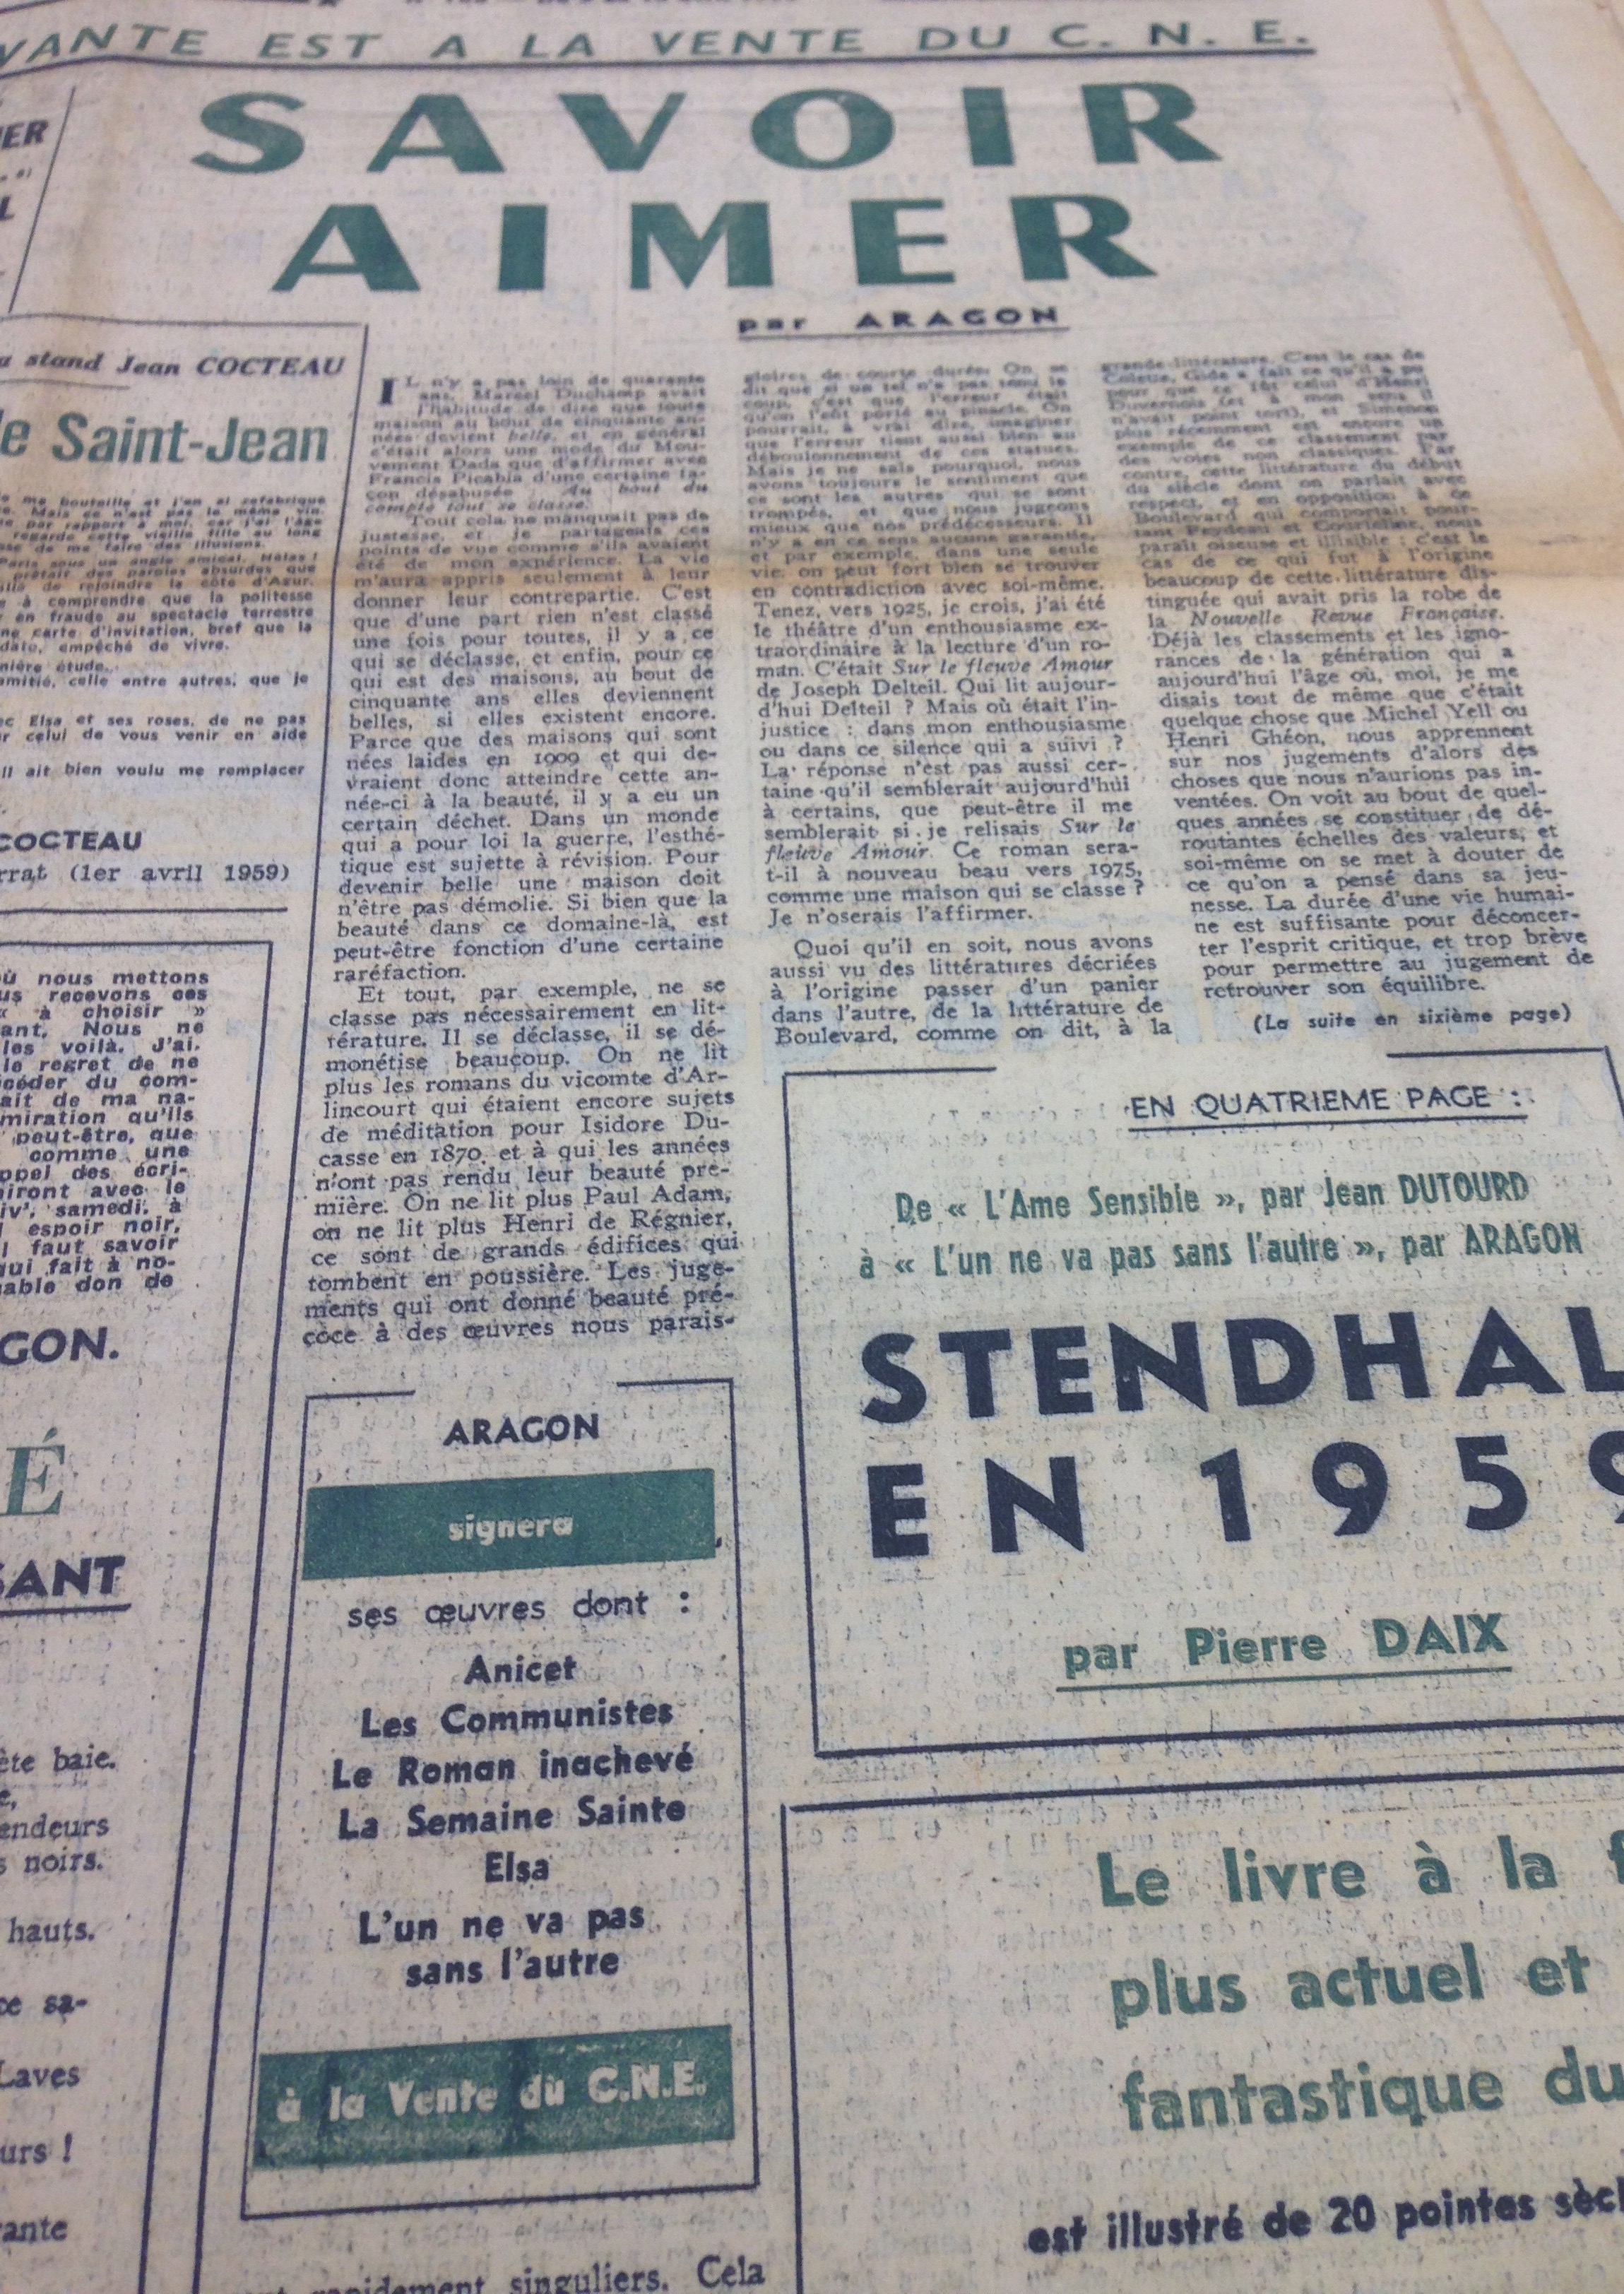
\includegraphics[width=0.33\textwidth]{savoiraimern708.jpg}
	\caption{\cite{savoiraimer}}\label{fig:Savoiraimer}
\end{figure}


Dans un troisième temps, à la lumière de la corrélation du travail esthétique et du message politique dans \emph{Les Lettres françaises}, il convient de mesurer le rôle de cet aspect du lyrisme révolutionnaire dans le traitement du réalisme socialiste. Cette notion dont Aragon se fait le grand représentant avec ses oeuvres romanesques du \emph{Monde réel} en France vient de ses nombreuses lectures et voyages en URSS. L'oeuvre oeuvre littérature, comme les arts en général, se conçoit comme le miroir de la société du point de vue du prolétariat. L'évolution du réalisme socialiste dans \emph{Les Lettres françaises} est particulièrement retrace son succès jusqu'à sa tentative de sauvegarde révélateur lorsque Arago doit peu à peu y renoncer, surtout après 1956. Avec les révélations du Rapport de Khrouchtchev, le modèle de Staline désacralisé. Cependant, le réalisme socialiste, lui, met du temps à s’éteindre complètement, notamment dans les articles de critique d’Aragon. 

	 Aragon publie son article \emph{Savoir aimer}\footcite{savoiraimer} un an après une autre grande enquête, celle déjà évoquée de 1958 : \emph{Qu’est-ce que l’avant-garde en 1958 ?}\footcite{avantgarde}. Les influences du sujet sur cet article de 59 sont manifestes : Aragon semble répondre indirectement au sujet lorsqu’il revient sur son expérience dada : \enquote{c’était une mode du Mouvement Dada que d’affirmer avec Francis Picabia d’une certaine façon désabusée : \emph{Au bout du compte tout se classe}.}



 Mais un autre élément intervient pour évoquer ces \oe{}uvres hors-normes devenues académiques, celle de l’identité :  
 \begin{quote}
  Mais je ne sais pourquoi, nous avons toujours le sentiment que ce sont les autres qui se sont trompés, et que nous jugeons mieux que nos prédécesseurs. Il n’y a en ce sens aucune garantie, et par exemple, dans une seule vie, on peut fort bien se trouver en contradiction avec soi-même.\footcite{savoiraimer}\end{quote}

	Est-ce qu’on peut voir dans cette reconnaissance d’\oe{}vres contradictoires chez un même individu une possible mise à distance avec le réalisme socialiste ? Toujours est-il qu’à la fois en partant de ses convictions au temps de sa jeunesse et cette conception d’une identité altérée, Aragon semble revenir pourtant à son passé dada plutôt qu’il ne s’en éloigne. Cette logique d'association d'idées par  « classement » poursuit le procédé de ces mouvements artistiques, mais s'inscrit aussi dans la philosohphie de l'identité mouvante : \enquote{Et tout, par exemple, ne se classe pas nécessairement en littérature. Il se déclasse, il se démonétise beaucoup.}\footcite{savoiraimer}

Ce procédé du classement, face aux changements et aux revirements du  classement des oeuvres, ce serait en somme une exploration de soi. Et, vis-à-vis des variations qui constituent un individu à travers les années,  Aragon suggère un vertige de l’identité, qui esr aussi finalité de la critique : 

\begin{quote}
 On voit au bout de quelques années se constituer de déroutantes échelles de valeurs, et soi-même on se met à douter de ce qu’on a pensé dans sa jeunesse. La durée d’une vie humaine est suffisante pour déconcerter l’esprit critique, et trop brève pour permettre au jugement de retrouver son équilibre.\footcite{savoiraimer}   
\end{quote}
 

	 On retrouve cette dimension fondamentale du temps, avec ses changements de perspectives depuis la jeunesse. L’entre-deux du temps ne peut aboutir qu’au vertige de la critique, et non au lieu commun de la critique qui se situerait plutôt dans la distanciation, le juste recul. Il peut paraitre paradoxal que l’article s’achève en éloge du réalisme socialiste, alors qu’à cette période Aragon commence à se tourner vers une autre conception du réalisme, qui n’est pas sans rappeler celui de Masson lorsqu’il peint ou dessine les hommes. Le verbe \emph{aimer} ,porté par le titre \emph{Savoir aimer},  plusieurs fois marqué par un italique de soulignement, se substitue par cette distinction typographique à « critiquer ». Savoir aimer, c’est savoir véritablement critiquer :  

     \begin{quote}
       Je pense, pour ma part, que le goût est une chose essentiellement positive. Que la critique devrait, en matière de littérature, être une sorte de pédagogie de l’enthousiasme. Qu’un vrai critique est celui qui apprend à \emph{aimer}, et attention ! j’emploie toujours verbe aimer au sens fort, j’entends ici que les critiques ne font pas leur métier, parce qu’on ne les voit jamais les yeux cernés pour avoir lu un livre, même quand ils en disent du bien.\footcite{atraversgaleries}    
     \end{quote}


	 Cette conception très lyrique de la critique, avec pour essence l’idée d’ \enquote{aimer}, est donc très proche de celle de Masson critique de Baudelaire comme critique dans l’article de 1968, neuf ans plus tard. Aragon et Masson partagent cette idée fondamentale d’une subjectivité du critique qui perdrait toute distance avec le sujet pour au contraire se plonger dans le vertige que procure l’\oe{}uvre. Comme chez Masson, pas seulement dans ses conceptions mais aussi dans son art, Aragon associe à cette exigence mentale une conséquence physique, due à l’obsession du critique sur le sujet, qui se répercuterait sur le système nerveux. Cet entrelacement de la pensée et du physique conduit logiquement à la métaphore de l’acte sexuel, : \enquote{Et personne ne songe à vous traiter d’impuissants, parce qu’on ne vous entend pas crier, quand vous lisez les romans ou les nouvelles de ce temps-ci. Il m’arrive de penser que c’est pour le moins étrange.}\footcite{savoiraimer} La métaphore est intéressante si l'on se rappelle que le l'érotisme valait comme symbole de liberté totale dans \emph{Le Con d'Irène}. 

     	Une révolution intérieure, comprise comme retournement des sens, doit envahir le critique, avec cette image insaisissable du cri. La même image du cri que Masson figure pour représenter la révolte paysanne. Comme Masson le revendiquera quelques années plus tard, Aragon encourage la passion que devrait susciter la critique, la prise de risques du jugement : \enquote{Bien parler d’un livre c’est peu. Il faut encore le situer. Oser dire, ceci restera}.\footcite{savoiraimer}

 Or, ce choix de déterminer ou pas la destinée d’une \oe{}uvre peut déjà se concevoir comme un choix politique. Celui d’anticiper, selon le jugement de valeur, une vision à long terme de l’oeuvre sur le sens politique. Elle se confirme avec cette « envie partisane » selon l’expression d’Aragon qui implique le geste du choix, en  particulier ce rôle crucial du critique, celui qui peut décider si le sort d’une \oe{}uvre se prolonge dans le temps : 

\enquote{ce mécanisme indémontable de l’art, par quoi se fonde la grandeur de l’oeuvre, et son droit à ne pas mourir}\footcite{savoiraimer} Le lyrisme de l’argumentation n’est pas seulement théorique, il est aussi typographique : Avec l’italique déjà abordé du verbe \enquote{aimer} qui insiste ainsi sur la force donnée au mot, mais aussi avec les majuscules, où  \enquote{J’AIME les choses bien faites} est redoublé quelques lignes plus tard par \enquote{JE ne sais pas comment vous avez la tête faite, et de quoi elle est peuplée : pour moi, j’ai toute la vie porté en moi des images dont rien ne pourrait me séparer.}\footcite{savoiraimer}

Le lyrisme est clairement manifesté avec ces majuscules autour du \enquote{je} et du verbe sur l’expression des sentiments par excellence. Sans compter que le sens de ces deux phrases éloignées dans l’article tournent autour de la même notion, même si la seconde phrase est plus explicite : le lyrisme vient des images qui hantent le critique. Ce qui rappelle le rapport aux images du processus de l'écriture et du dessin automatique, selon les critères surréalsites, dont la création émanait de ce débordement d'images incontrôlées. 

	Et pourtant, c’est encore par une sauvegarde du réalisme socialiste qu’Aragon ponctue finalement, comme le lieu même de l’amour : 
\begin{quote}
  l’amour pour que je le ressente, que je le partage doit  être réel, et réaliste l’art qui le décrit, et que c’est l’étrange calomnie que de prétendre que si ce réalisme a le socialisme pour soleil l’amour s’y doit étioler, quand c’est au contraire cet \emph{idéal qui donne à l’histoire réelle, la force même de l’amour}.\footcite{savoiraimer}\end{quote}


Pour aboutir au réalisme socialiste, Aragon soit revenu sur les autres formes de réalisme du temps de sa jeunesse. En 1959, le réalisme socialiste va peu à peu dans ses \oe{}uvres laisser la place à une autre perspective du réalisme. Néanmoins, cette conception de la critique rejoint à bien des égards sa position de critique de poésie dans les fameuses \emph{Chroniques du Bel Canto} de 1946 : 

\begin{quote}C’est un phénomène auquel il ne semble pas que les critiques se soient arrêtés : l’éclectisme nouveau et bizarre de la poésie des derniers temps…Comment ne pas voir qu’il reflète, que notre poésie écartelée reflète les incertitudes de esprits, l’égarement social, le trouble de l’homme ? La poésie est le miroir brouillé de notre société. Et chaque poète souffle sur ce miroir : son haleine différemment l’embue.\footcite[p93]{belcanto}\end{quote}

 Aragon se distingue d'une certaine pratique de la critique très distante de son sujet, et par opposition transforme le critique lui-même en poète. Le poète et le critique sont conciliés par la métaphore du miroir qui lie la poésie à l'idée d'actualité, puisqu'elle reflète l'état des esprits des hommes. Le lyrisme est ainsi déjà introduit comme une condition du travail de critique :

\begin{quote}Il nous faut prendre comme un fait le bariolage des techniques poétiques l’habit d’Arlequin des faiseurs de nuages. C’est un signe. Et qui traduit des phénomènes mal connus, en eux-mêmes difficilement saisissables. Comme l’ombre du passant,lyrique, amplifiée, trahit parfois sur les murs ses intimes incompréhensibles pensées cachées.\footcite[p94]{belcanto}\end{quote}

Le lyrisme est perçu comme un état de l'homme, de ses tumultes intérieurs. Ce \enquote{miroir du réel} du travail de critique projette cette particularité de l'homme sur son objet. Cette position de la transition entre l'après-guerre et la guerre froide poursuivie jusque dans l'article de 1959 \emph{Savoir aimer} revitalise par le lyrisme le réalisme socialiste à bout de souffle.


	Cet article revendique l’entrelacement du lyrisme et d'une dimension politique le fait sur deux aspects : d'une part, une notion subjective propre au choix, celui de faire perdurer une oeuvre plutôt qu’une autre. Ce qui se rapproche d’une politique éditoriale dans les choix d’articles et la mise en page d’un numéro. En particulier pour le journal \emph{Les Lettres françaises}, qui, par sa position avant tout culturelle, est nourri en grande partie de critiques. C’est donc toute la ligne éditoriale du journal qui est explicitée dans l’article, son \enquote{envie partisane}et la recherche du vertige dans les agencements d’articles comme dans le choix des sujets. D’autre part, on peut concevoir cet article comme un entre-deux, ou plutôt un mouvement pris dans la réflexion d’Aragon à propos du réalisme socialiste : à la fois l’idée même du socialisme qui, chez Aragon, procure au lyrisme sa force subversive. Et, en même temps, des traces d’affinités pour une autre conception du réalisme font déjà pressentir les nouvelles réflexions romanesques en cours pour Aragon en tant qu’auteur. 

	

\subsection{Les échanges d'André Masson avec \emph{Les Lettres françaises }}

L’année 1959 semble être l’année de l’entre-deux, pour Aragon d’une part, mais pour Masson aussi, si l’on s’en tient à ses \oe{}uvres exposées au Salon de Mai\footcite{salondemai} en mai 1959 : \enquote{un André Masson plein de fougue qui illustre la transition entre le surréalisme et l’abstraction}, d’après Georges Boudaille. Un même mouvement de transition s’opère chez Aragon comme chez Masson, entre les élans de retours vers des affinités premières, et les prémices d’une réflexion autre qui émerge de cet entre-deux. Même si Boudaille qualifie de \enquote{fougue} la force des oeuvres expressives de Masson, la toile représentée sur la page dans l’article, \emph{Un couple dans la nuit}, revient dans un autre numéro pour illustrer un texte de Claude Durand. Toujours sur ce thème de l’entre-deux, entre le jour et la nuit, où le lyrisme du personnage qui erre dans les rues la nuit et revit des discussions de couples se manifeste plus comme un écho à la réflexion du narrateur qu’à une illustration : 


\begin{quote}
Ivresse des limites perdues. Mais, parce que je suis seul, aucune épouvante ne me saisit (c’est ce qui nous ressemble qui nous terrifie). L’angoisse ? Ce vide m’était encore tout à l’heure mon droit à la joie, presque une plénitude…A quoi est-ce que je crois ?\footcite{durand} 	
\end{quote}
% Mettre illsutration "Un couple dans la nuit".

\begin{figure}[H]
   \centering
   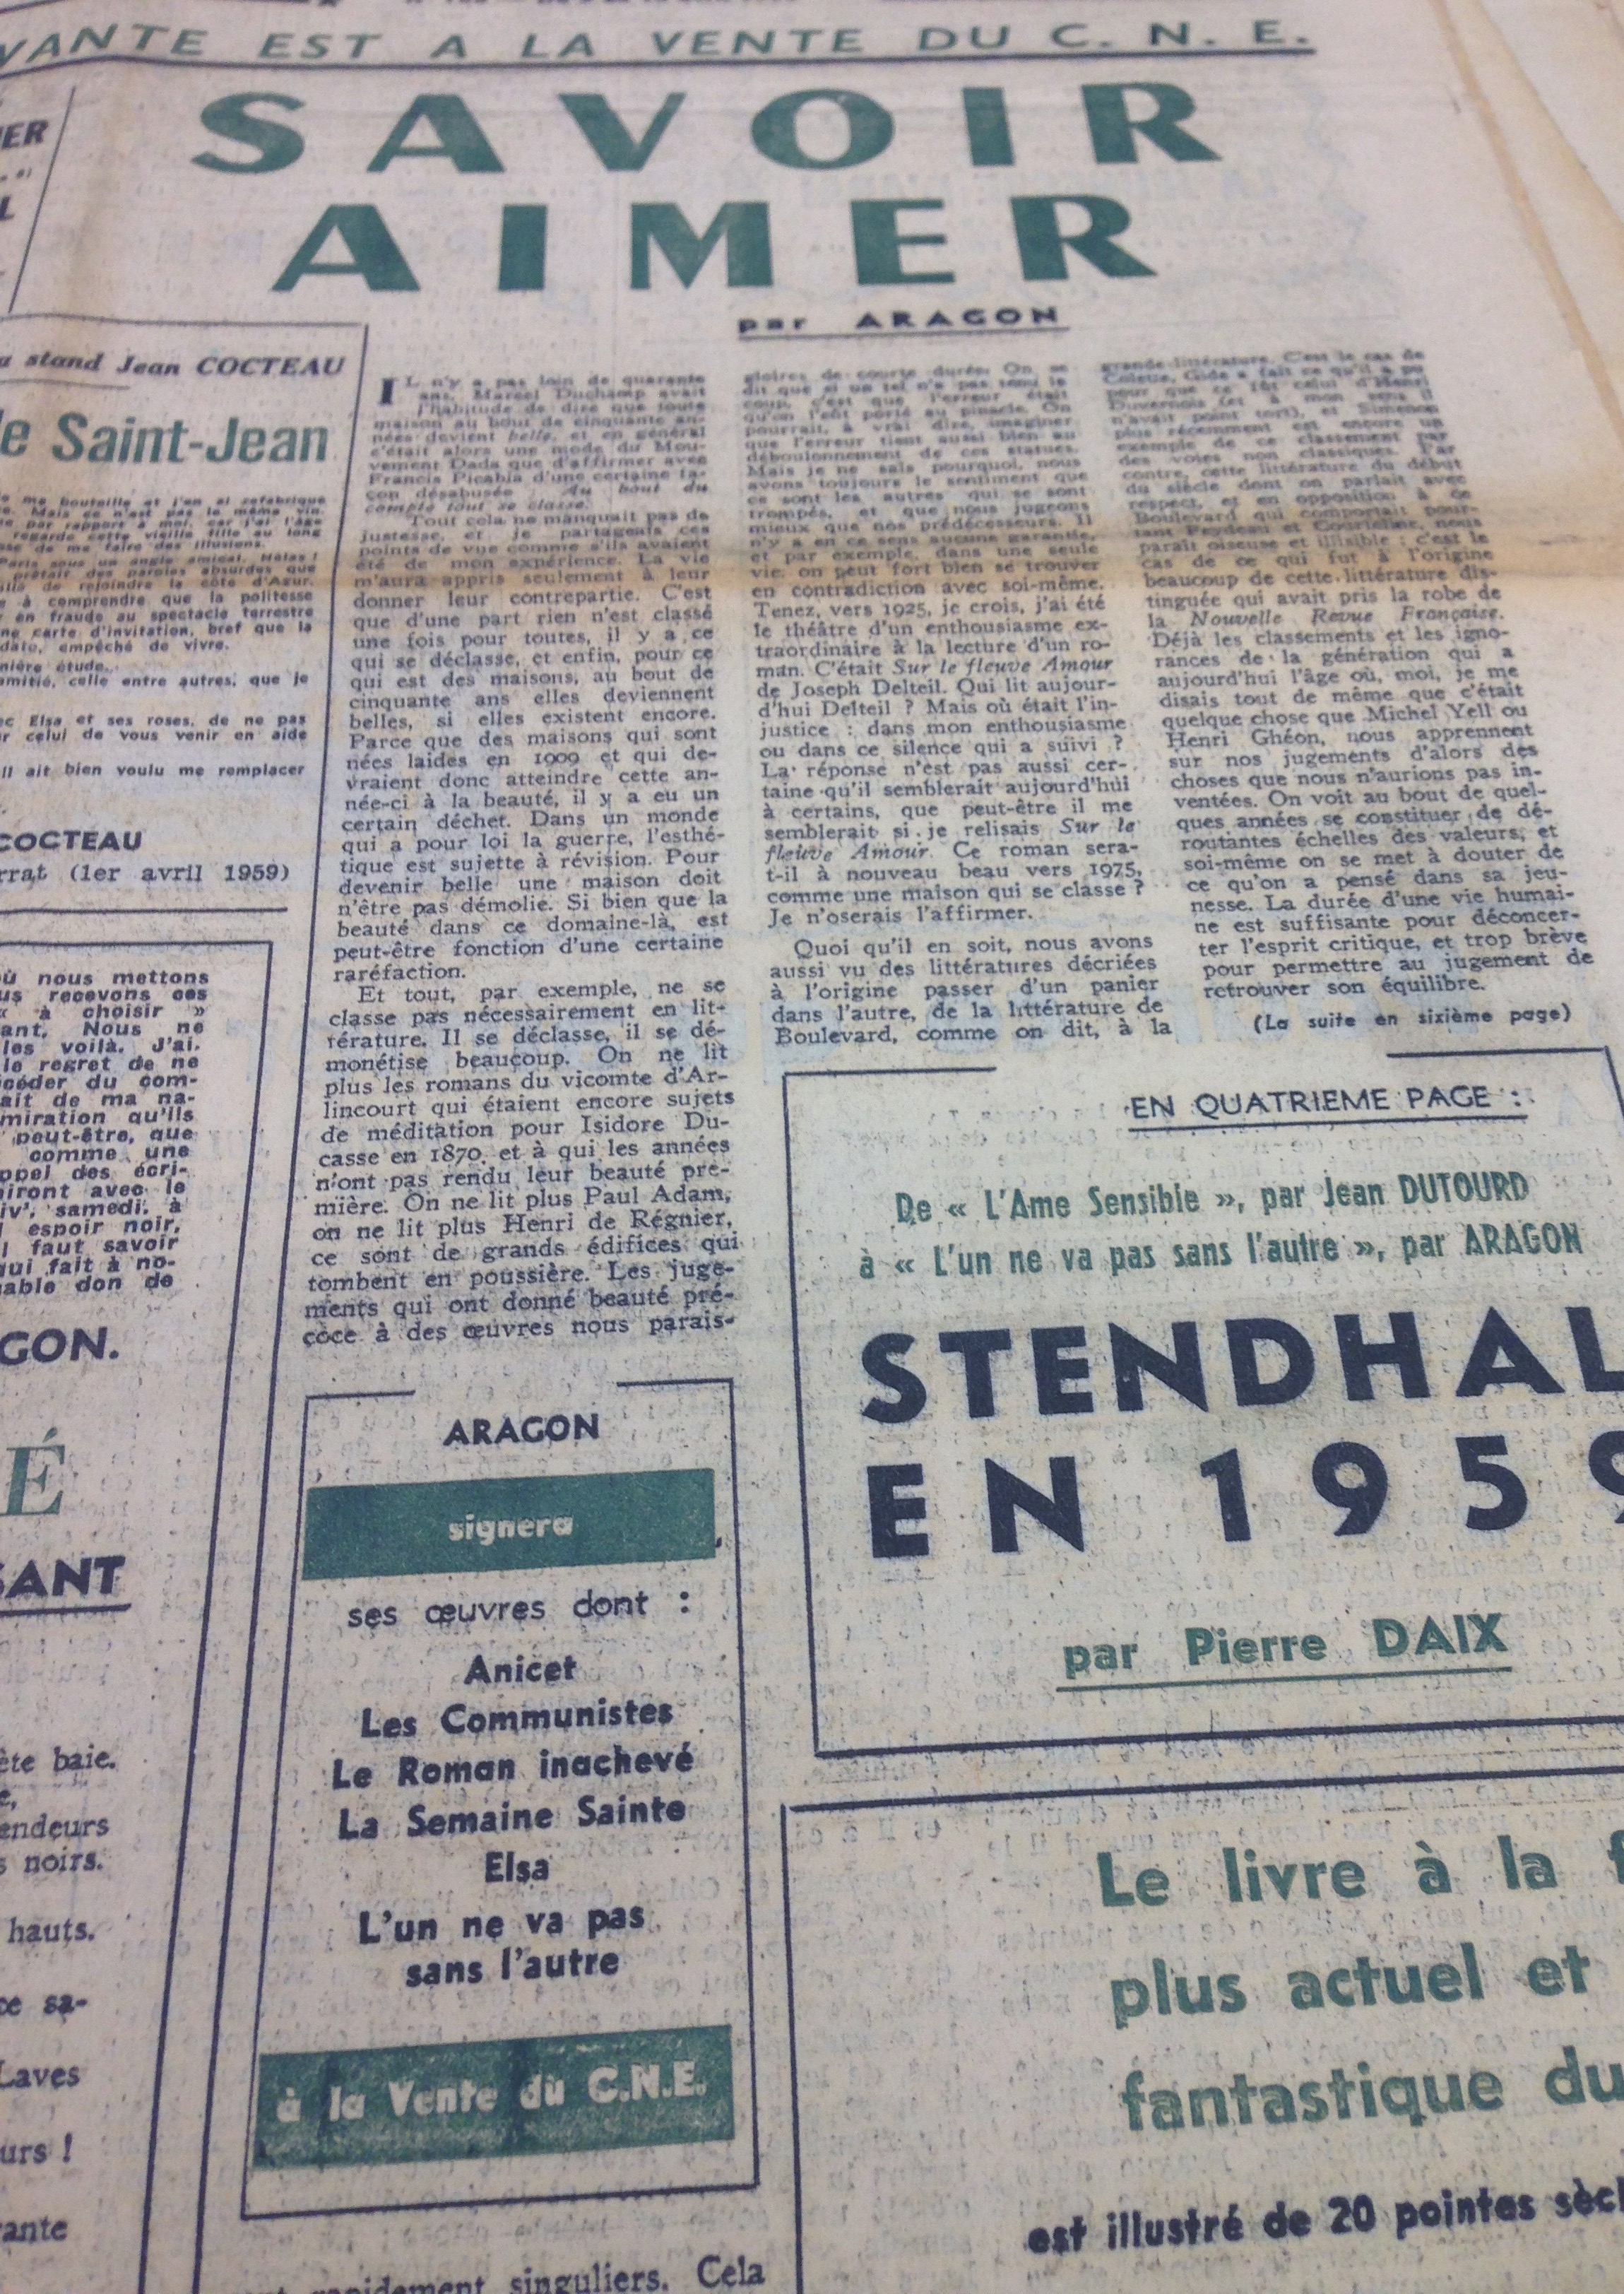
\includegraphics[width=0.33\textwidth]{savoiraimern708.jpg}
	\caption{\cite{savoiraimer}}\label{fig:Savoiraimer}
\end{figure}

 Or, l’angoisse, plus qu’un sentiment, est un véritable moyen d’expression dans l’art d’André Masson. Dans l’article de Georges Boudaille comme dans le texte de Claude Durand, le titre de l’oeuvre de Masson apparemment serein est ainsi qualifié par l’énergie et l’errance, thème romantique. Il est vrai que, si les silhouettes de l’homme et de la femme sont immédiatement perceptibles, c’est par leurs traits appuyés plutôt que par la représentation d’une chair. Leur main entrelacée, par un croisement de lignes, n’en figure qu’une seule. Paradoxalement, les lignes apportent l’érotisme à leur corps nu, de façon plus directe que s’il s’était agit d’une représentation réaliste et fidèle d’un homme et d’une femme. La force symbolique que procure les lignes pour former les corps nus rapprochent ce couple plus d’une Idée au sens symbolique, plutôt que de personnages, chargés de jouer un rôle quelconque dans l’oeuvre.  


De plus, Pierre Descargues qualifie l’esthétique d’André Masson de \enquote{réel fantastique} dans son article \emph{André Masson et le réel fantastique}\footcite{reelfantastique}. Aragon venait de  prendre l'année précédente la direction  de la rubrique \emph{Tous les arts}. Pierre Descargues y occupe conjointement avec Aragon une chronique, \emph{A travers les galeries}. Ainsi, tout comme d’autres chroniqueurs tels que Georges Boudaille ou Georges Besson, Descargues connaît intimement Aragon et André Masson. 

\begin{figure}[H]
   \centering
   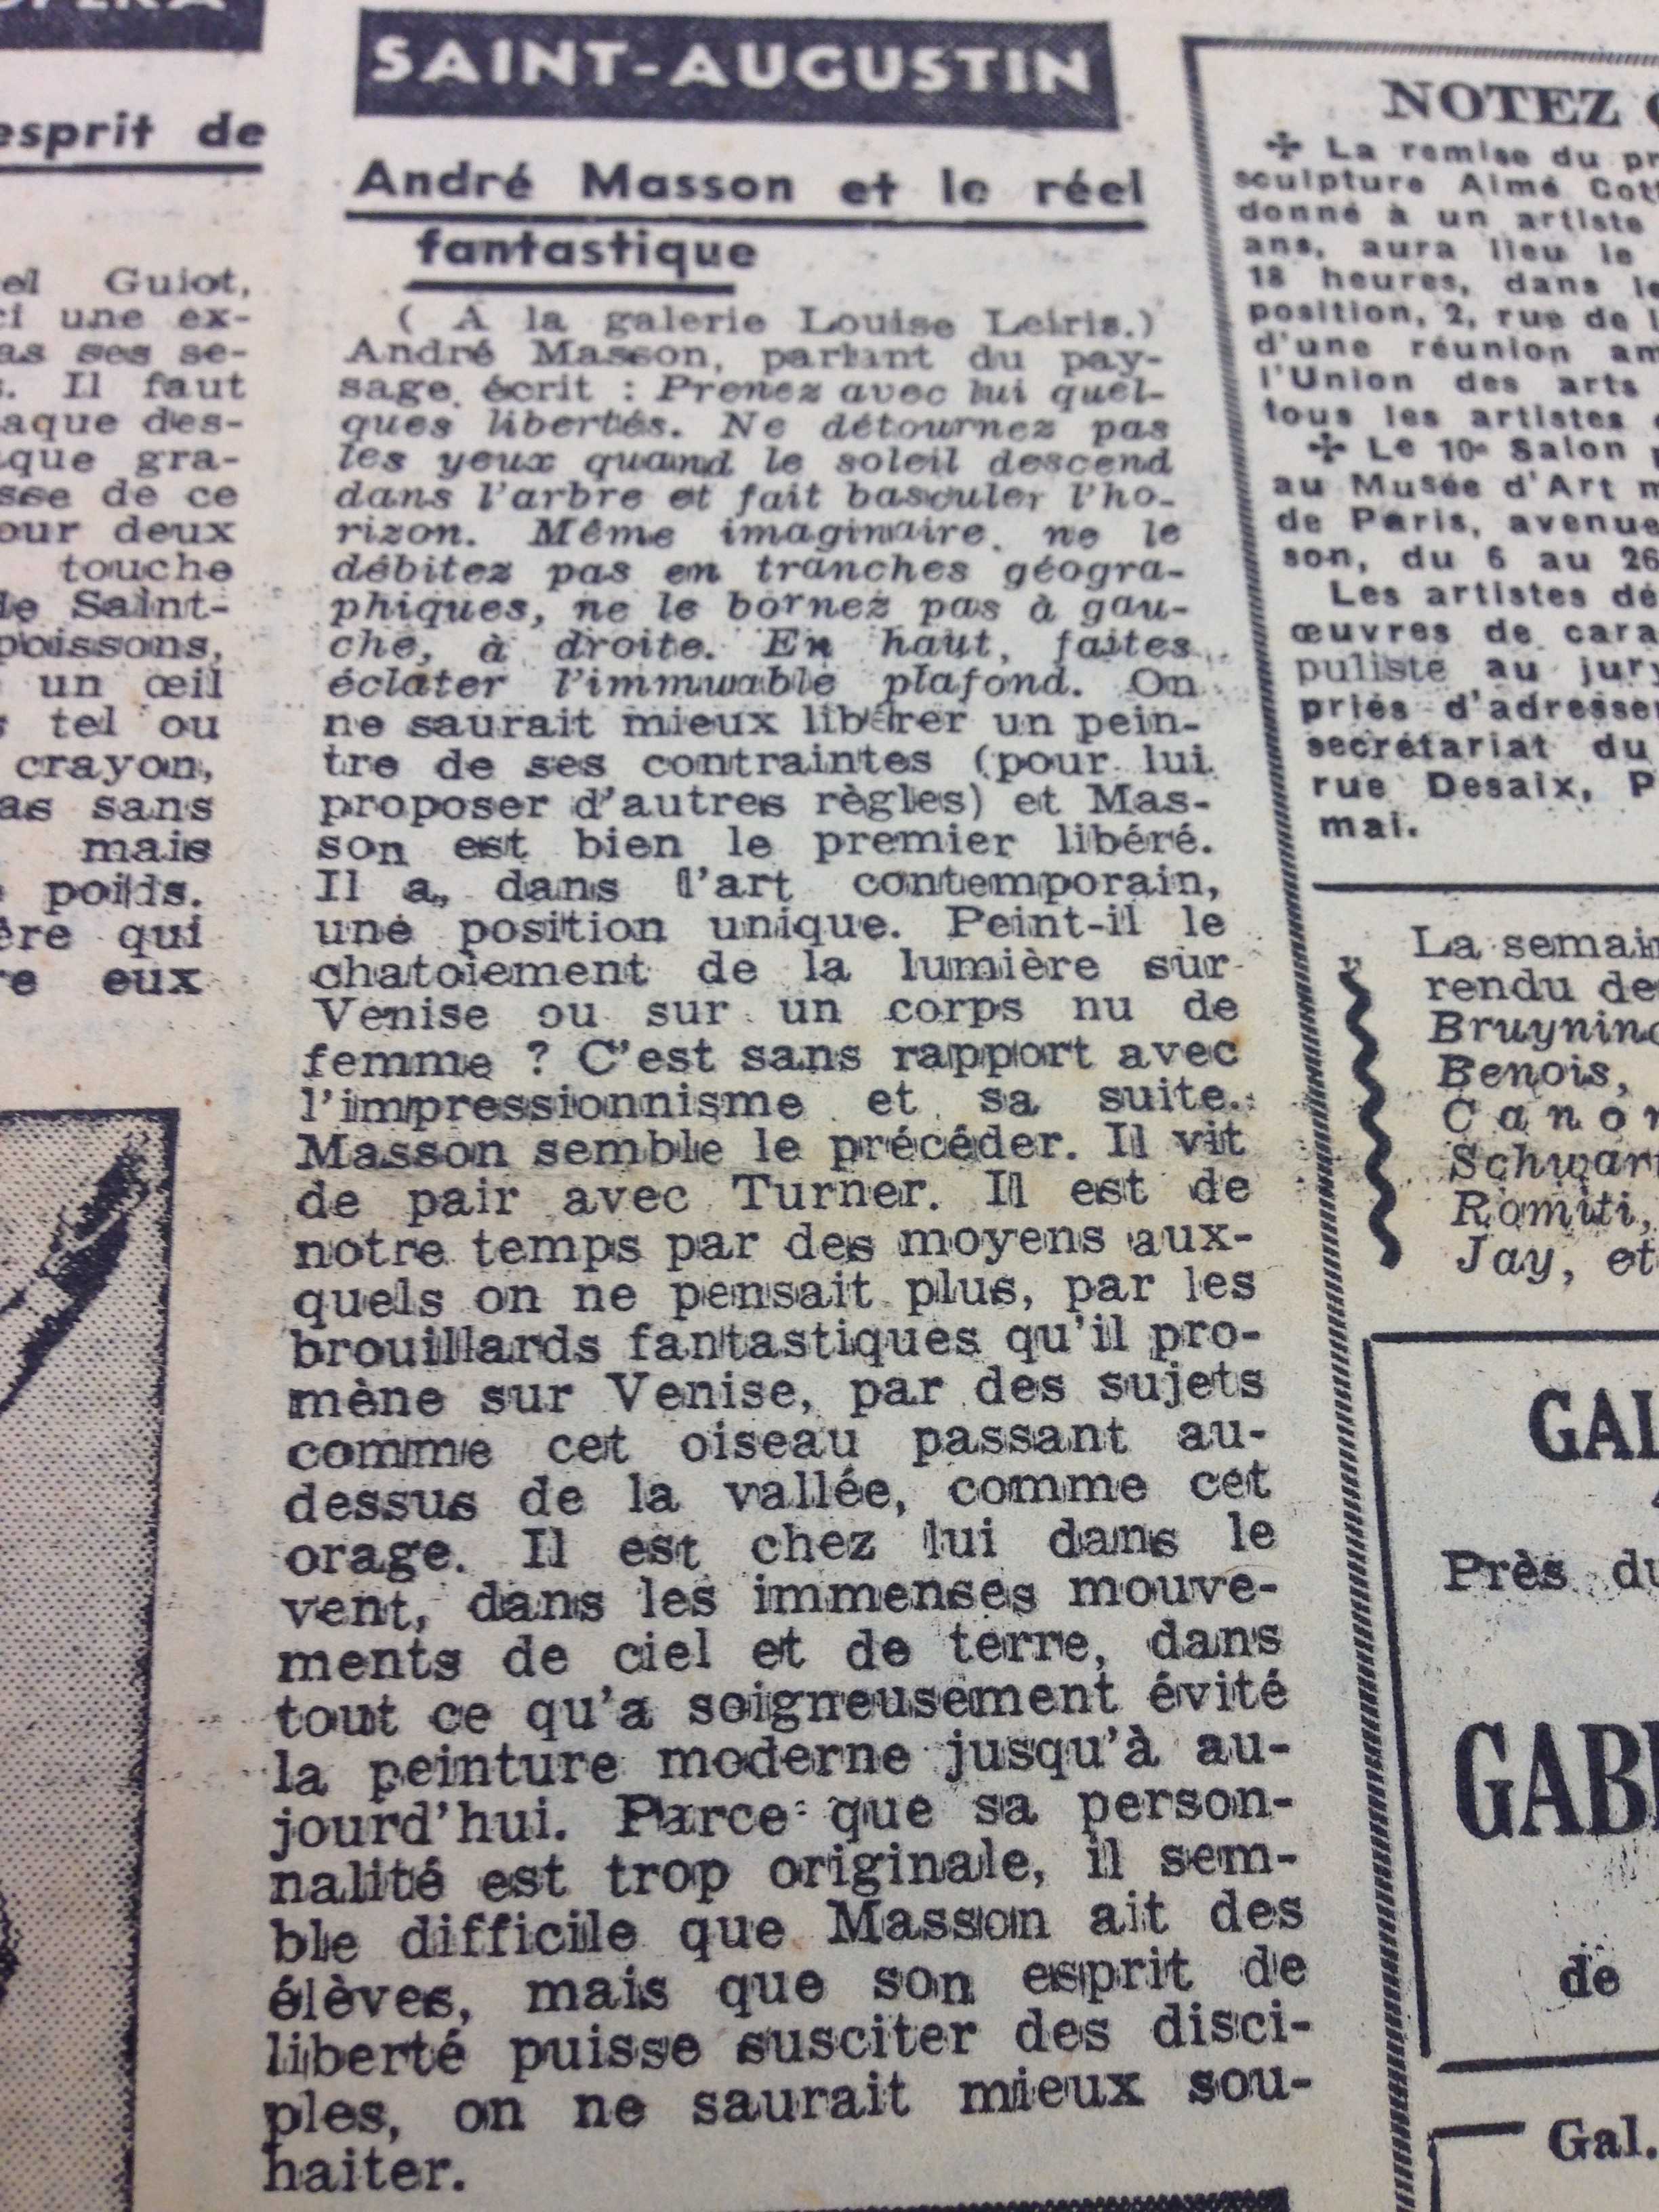
\includegraphics[width=0.33\textwidth]{textereelfantastiquen411.jpg}
	\caption{\cite{reelfantastique}}\label{fig:Articlereelfantastique}
\end{figure}

\begin{figure}[H]
   \centering
   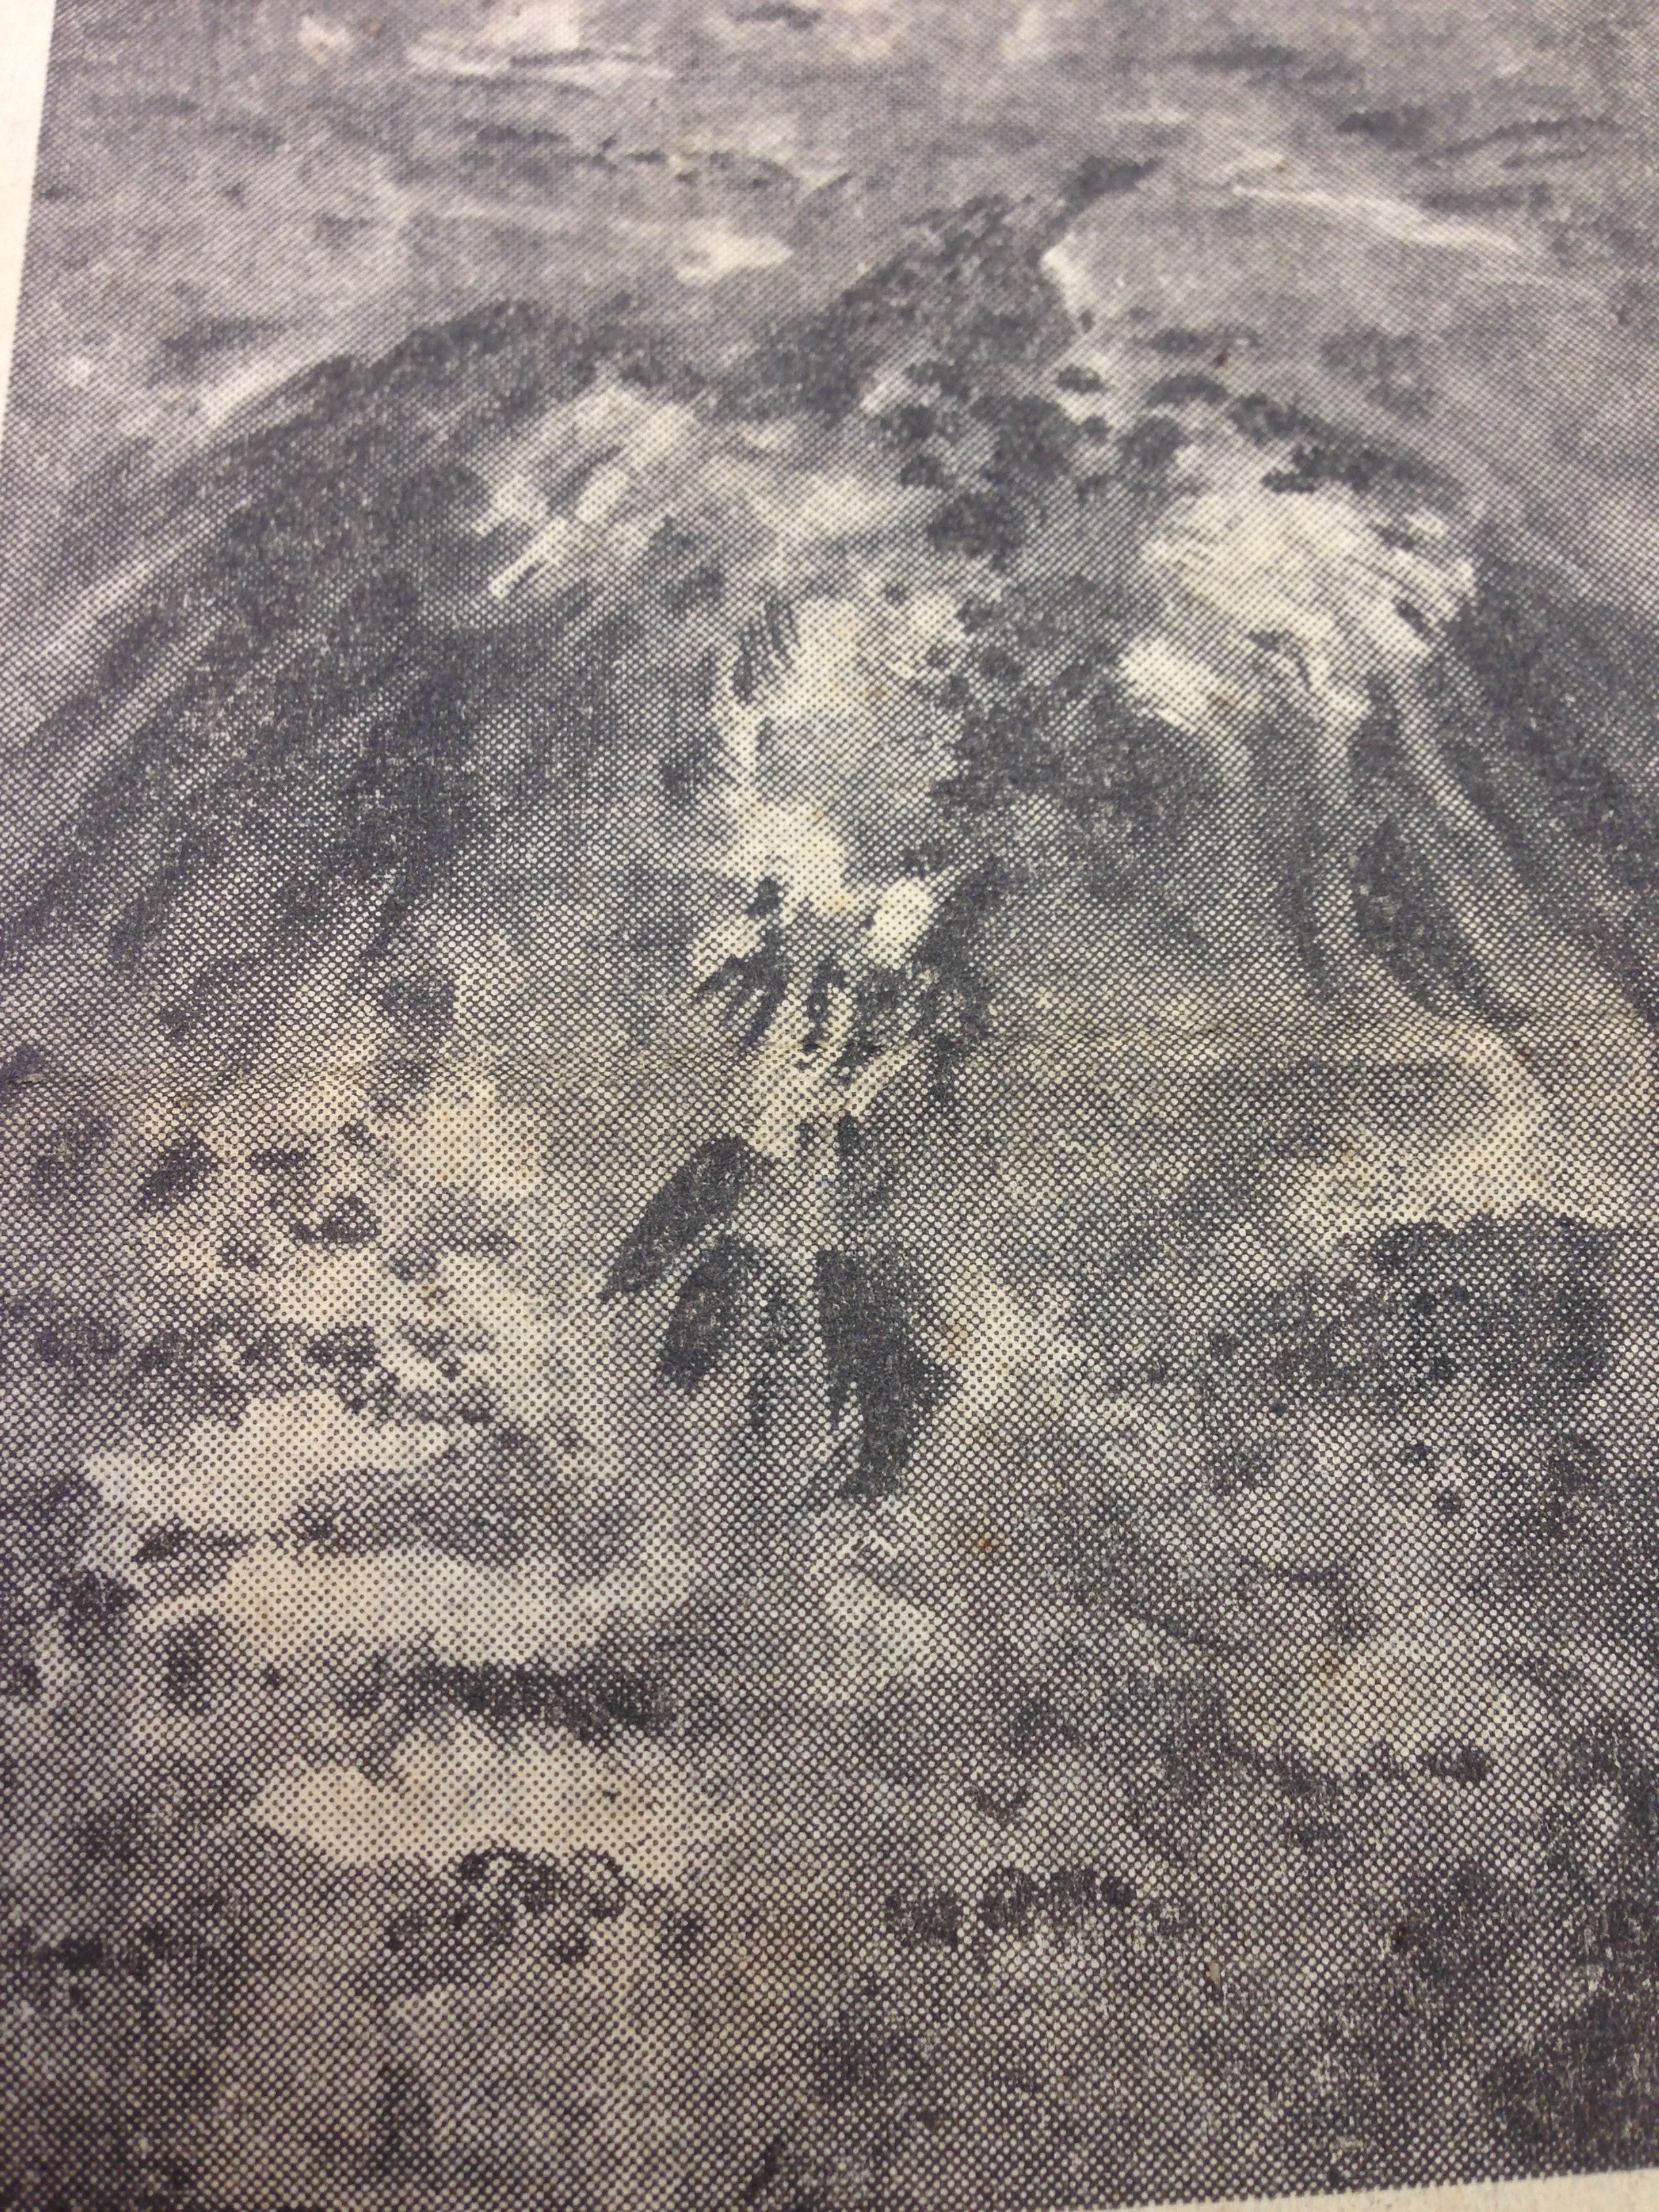
\includegraphics[width=0.33\textwidth]{reelfantastiquen411.jpg}
	\caption{\cite{reelfantastique}}\label{fig:Imagereelfantastique}
\end{figure}


	Il s'avère que, au début des années 50, la politique éditoriale est toujours tournée vers une politique de paix dans un contexte de guerre froide, avec le symbole des colombes massivement représenté depuis 1948, et la défense du réalisme socialiste. Est-il possible que cette page de la rubrique des Arts propose implicitement un croisement entre le réalisme socialiste et le réel fantastique ? En ouvrant son article avec des mots de Masson à propos de l’art de figurer le paysage, c’est le lien étroit entre le réel et l’imaginaire qui est pointé : 

 \begin{quote}
Prenez avec lui quelques libertés. Ne détournez pas les yeux quand le soleil descend dans l’arbre et fait basculer l’horizon. Même imaginaire, ne le débitez pas en tranches géographiques, ne le bornez pas à gauche, à droite. En haut, faites éclater l’immuable plafond.\footcite{reelfantastique}\end{quote}

	 En somme, selon Descargues, Masson revendique le contraire de l’ordre. Non seulement il préconise à l’artiste des \enquote{libertés}, mais la Nature elle-même comporte une part subversive pour lui. Ce qui explique le geste de l’artiste subversif aussi pour Masson qui ne recherche pas la mimétique de la Nature,refuse l'ordre classique et aligné de la composition, pour au contraire \enquote{éclater l’immuable plafond}.

	  Cette idée de jaillissement rappelle même plus l’abstraction que la figuration, à ceci près qu’une fois encore il s’agit de se détourner du mimétique pour l’expression de la Nature, et son éventuel réalisme véritable. Or, ce réalisme ne peut être possible qu’avec ce facteur fantastique, ce qui selon Descargues est plutôt tourné vers l’idée de l’imaginaire et de l’onirique. On relève donc la dimension paradoxale d’un réalisme qui advient par l’imaginaire et le rêve dans le but de figurer l’essence de la Nature, ce qu’elle veut signifier, plutôt que sa copie. C’est qui fait écrire au critique que Masson est en somme un insaisissable : 
 
En outre, l’allusion à Turner est d’autant plus parlante pour les quelques lignes que Masson lui avait sacré au début de cette même année 1952 (clin d’oeil de Descargues ? ) : \enquote{Disparition de la pesanteur}. Ces propos sur Turner sont essentiels pour comprendre qu’en refusant le mimétique, Masson a aussi délibérément choisi de de composer avec des lignes plutôt qu’avec l’effet de masse. La forme faite de lignes fait deviner plus qu’il ne le signifie directement, puisque le sujet est dépossédé de sa masse corporelle. Sans compter qu’on peut considérer Turner comme faisant de l’impressionniste avant l’heure, ce qui fait de son mouvement aux couleurs chaudes un art insaisissable à son époque d’une façon similaire à André Masson. 

Il  s’agit de constater comment le \enquote{réel fantastique} de Masson  croise le projet du réalisme socialiste qui est celui de la politique éditoriale. Sa part de romantisme révolutionnaire est étroitement liée au réalisme socialiste. 


	Reynald Lahanque offre une première piste sur les motivations éditoriales du journal, et plus précisément d’Aragon comme responsable de cette rubrique Tous les Arts, quelques mois avant d’être officiellement directeur de tout l’hebdomadaire, dans sa thèse sur le réalisme socialiste en France : 

\begin{quote}
Le terme même de \enquote{réalisme socialiste}se rencontre assez rarement dans \emph{Les Lettres françaises}, mais la problématique que le terme recouvre y est très largement présente. Dirigé dans les faits par Aragon et Daix, l'hebdomadaire culturel fait toute sa place, sur un plan plus général, aux thèses et aux thèmes de la propagande communiste de la guerre froide. Il garde en même temps l'ambition de toucher un public plus large que celui des militants, et conserve des collaborateurs moins engagés politiquement et capables d'élargir la gamme de ses centres d’intérêt. \footcite{}\end{quote}

	Comme pour toute politique, le choix éditorial met en valeur un élément au détriment d’un autre. A dessein de ne pas se limiter à un lectorat proche l’appareil du PCF, le terme « réalisme socialiste » subit un profond paradoxe : Il est plus que jamais à l’ordre du jour dans ce contexte de guerre froide, tout en restant discret en raison de sa connotation immédiatement politique. On retrouve ici ce qu’Aragon revendique quelques années plus tard en 59 comme l’\enquote{envie partisane}\footcite{savoiraimer}, essence du travail de critique. 

Or, si l’\enquote{envie partisane} existe déjà en 1952, elle ne doit pas paraître invasive, puisqu’elle définit une idéologie précise en contradiction avec la politique éditoriale d’ouverture à un plus large public. Face à cette contradiction entre les attentes politiques et les attentes éditoriales, le mot d’ordre qui vient à la place envahir le journal, mais qui sous-tendrait au réalisme socialiste, c’est le mot \enquote{Paix}, omniprésent depuis les années 48, et d’une portée large, voire unanime.À peine quelques années après la Seconde Guerre Mondiale, qui voudrait encore la guerre ? Mais, sur le plan artistique, le \enquote{réel fantastique} pour désigner l’art d’André Masson pourrait lui-même aboutir idéologiquement à une forme dérivée du réalisme socialiste. Avec, cependant, une qualification onirique de ce réalisme qui n’apparente pas l’expression directement à une théorie politique. 

Jusqu’à son terme, la dimension proprement lyrique de l’article de Descargues, avec cette métaphore du vent qui incarne à la fois les représentations et la méthode de Masson, semble appuyer la rêverie et s’éloigner de tout aspect politique : \enquote{Il est allé chez lui dans le vent, dans les immenses mouvements de ciel et de la terre, dans tout ce qu’à soigneusement évité la peinture moderne jusqu’à aujourd’hui. Parce que sa personnalité est trop originale.}\footcite{atraversgaleries} On est apparemment plus proche des \emph{Rêveries d’un promeneur solitaire} de Rousseau que du réalisme socialiste. 

	Cependant, la liberté est aussi un concept politique fondamental, et c’est bien celle-ci qu’aspire à faire rêver au lecteur le mouvement lyrique. L’adverbe \enquote{trop} pour conclure sur la dimension atypique de Masson ne peut pas être anodine. En substance, l’art d’André Masson est un débordement. Peut-on alors supposer que le \enquote{réel fantastique} est un mode de représentation du réalisme socialiste ? La question peut trouver des réponses contradictoires, dans cette année 1952, où, dans un article d’éloge à la remise du Prix Staline au roman \emph{Le Premier choc} d'André Stil\footcite{prixstaline}, Aragon rappelle, non sans apparenter cette définition en partie à Staline, ce qu’est le réalisme socialiste : 
	\begin{quote}
	Le réalisme socialiste, étant la méthode de base de la littérature et de la critique soviétique, exige de l’artiste une représentation véridique, historiquement concrète de la réalité dans son développement révolutionnaire. De plus, le caractère véritable et historiquement concret de cette représentation artistique de la réalité doit se combiner avec le devoir de transformation idéologique et d’éducation des masses dans l’esprit du socialisme.\footcite{prixstaline}\end{quote}
	
	 Une telle définition demanderait à se poursuivre par la définition cette fois du socialisme. Est-il d’ailleurs le même en URSS qu’en France, si on prend en compte le fait que la politique du parti communiste diffère sur certaines caractéristiques d’un pays à l’autre ? Reynald Lahanque pointe d’ailleurs la pratique du réalisme socialiste d’Aragon dans les romans du \emph{Monde réel}. Il les juge peu représentatifs des héros communistes-types du réalisme socialiste et de scénario d’apprentissage grâce au Part. Mais, vis-à-vis du \enquote{réel fantastique}, ce qui est en jeu,c’est la question de la représentation \enquote{véridique, historique, concrète de la réalité} telle que l'exige le réalisme socialiste. 

 Cet appel à la figuration manifeste et plutôt naturaliste contraste donc avec l’aspect \enquote{fantastique} de Masson. Cependant, si l’on s’arrête aux louanges d’Aragon sur \emph{Le Premier choc}, l’aspect très pragmatique établi dans cette définition du réalisme socialiste est substitué à une autre forme de réalisme : \enquote{Je veux parler de sa façon de décrire les personnages. Ou plutôt de ne pas les décrire}.\footcite{prixstaline} On commence par cette suggestion d’une autre forme \enquote{concrète} du réel qui ne serait pas une forme naturaliste à se rapprocher de la conception d’André Masson sur la représentation des paysages. Ce constat sur lequel s’appuie Aragon repose sur un fondement analogue au « réel fantastique » de l’artiste de Descargues : il s'agit de figurer non le sujet en tant que tel, mais ce qu’exprime le sujet : \enquote{Parce que justement, ici, la ressemblance ne tient  pas à un \emph{trait} qui se répète. Mais à la nature complexe de l’homme décrit.} Cette phrase sur l’\oe{}uvre de Stil pourrait se confondre avec celles de Masson : le peintre revendique une idéologie esthétique contre le sujet figé du mimétique, et manifeste sa recherche de l’essence du sujet, sa nature. 


	Un tel projet ne peut que reposer en partie sur l’imagination comme moyen de représentation. Ce qu’Aragon dans ce même article nomme le \enquote{typage d’âme} : \enquote{Les personnages du \emph{Premier Choc} sont socialement définis et individuellement distingués par ce que j’appellerai le \emph{typage d’âme}. C’est à leur façon de penser, c’est au contenu de leur pensée, socialement définie- et au caractère de chacun, que l’auteur a fait appel pour fixer leurs images.}. Cette analogie entre \emph{Le premier choc} de Stil et l’\oe{}uvre d’André Masson illustre la conviction d’Aragon au début de l’article qu’avec le réalisme socialiste, on peut parler de la littérature pour évoquer l’art, et réciproquement.  Le choix stylistique de Stil est d’ailleurs bien plus qu’un détail pour Aragon, et peut-être est-ce même l’un des fondements qui permet à cette notion son \enquote{ développement révolutionnaire} comme finalité, d’après sa définition : \enquote{“Ce qui se passe dans leurs yeux est plus important que leur couleur“…Je vous dis que cette page que j’ai recopiée a valeur de manifeste.} La fonction poétique de la phrase n’est pas anodine, c’est même elle qui lui confère une forme de maxime. Le \enquote{typage d’âme} pourrait donc être le fil directeur à la fois du réalisme socialiste et des convictions d’André Masson. Dès lors, la notion de concret est complètement redessinée. Cependant, si une nature révolutionnaire associée à une forme lyrique est commune à la fois à l’article d’Aragon sur Stil et au réel fantastique de Masson, on peut distinguer cette finalité révolutionnaire : le réalisme socialiste comporte dans la suite de sa définition une valeur éducative, qui est peut-être l’élément que l’on ne retrouve pas de façon évidente dans le \emph{Monde réel}. André Masson réclame qu'on fasse \enquote{éclater l’immuable plafond}, mais pas à dessein nécessairement éducatif, tout au contraire. Dans l’exemple du paysage, celui-ci a la forme du fameux que l’on retrouve symbolisé dans beaucoup de ses oeuvres, et cette expression du mouvement est une finalité en soi. La rationalisation du mouvement ne semble ni attendue ni souhaitée. 

Or, la définition du réalisme socialiste dans cet article d’Aragon pourrait comporter le paradoxe de sa finalité : \enquote{Le développement révolutionnaire} pourrait se concilier avec la seconde partie de la définition, \enquote{se combiner avec le devoir de transformation idéologique et d’éducation des masses dans l’esprit du socialisme.} Si le mouvement révolutionnaire comporte en substance une notion de liberté, rattachée par André Masson dans l’article sur le réel fantastique et à son art en général, celui-ci semble difficilement rentrer dans la finalité de contrôle et d’ordre que sous-entend \enquote{l’éducation des masses}. C’est pourquoi, tout en rappelant lui-même cette définition et l’influence de Staline, si l’on évoque les oeuvres du \emph{Monde réel}, on peut se demander si les oeuvres réalistes socialistes d’Aragon n’ont pas elles-mêmes tant recherchées \enquote{l’éducation des masses} que le \enquote{développement révolutionnaire} des personnages. 

\subsection{Comparaison des articles \emph{ Réalisme socialiste pas mort}d' Aragon \emph{A travers les galeries} de Pierre Descargues}

	Croiser un article de critique littéraire et un autre sur les expositions dans les galeries d’art en 1957 met en valeur la grande influence de la foi communiste du directeur du journal, Aragon, cette année-là. Les livres vont êtres analysés, comme l’indique très clairement Aragon dans son titre \emph{Réalisme socialiste pas mort}\footcite{realsoc}, son commentaire sur les livres \enquote{L’Homme ne vit pas seulement de pain}, de Vladimir Doudintsev, et de \emph{L’Or} de Boris Polevoï se fait dans l’éclairage du réalisme socialiste. Ce qui n’est pas anodin : Les oeuvres sont louées pour leur valeur réaliste socialiste. 

\begin{figure}[H]
   \centering
   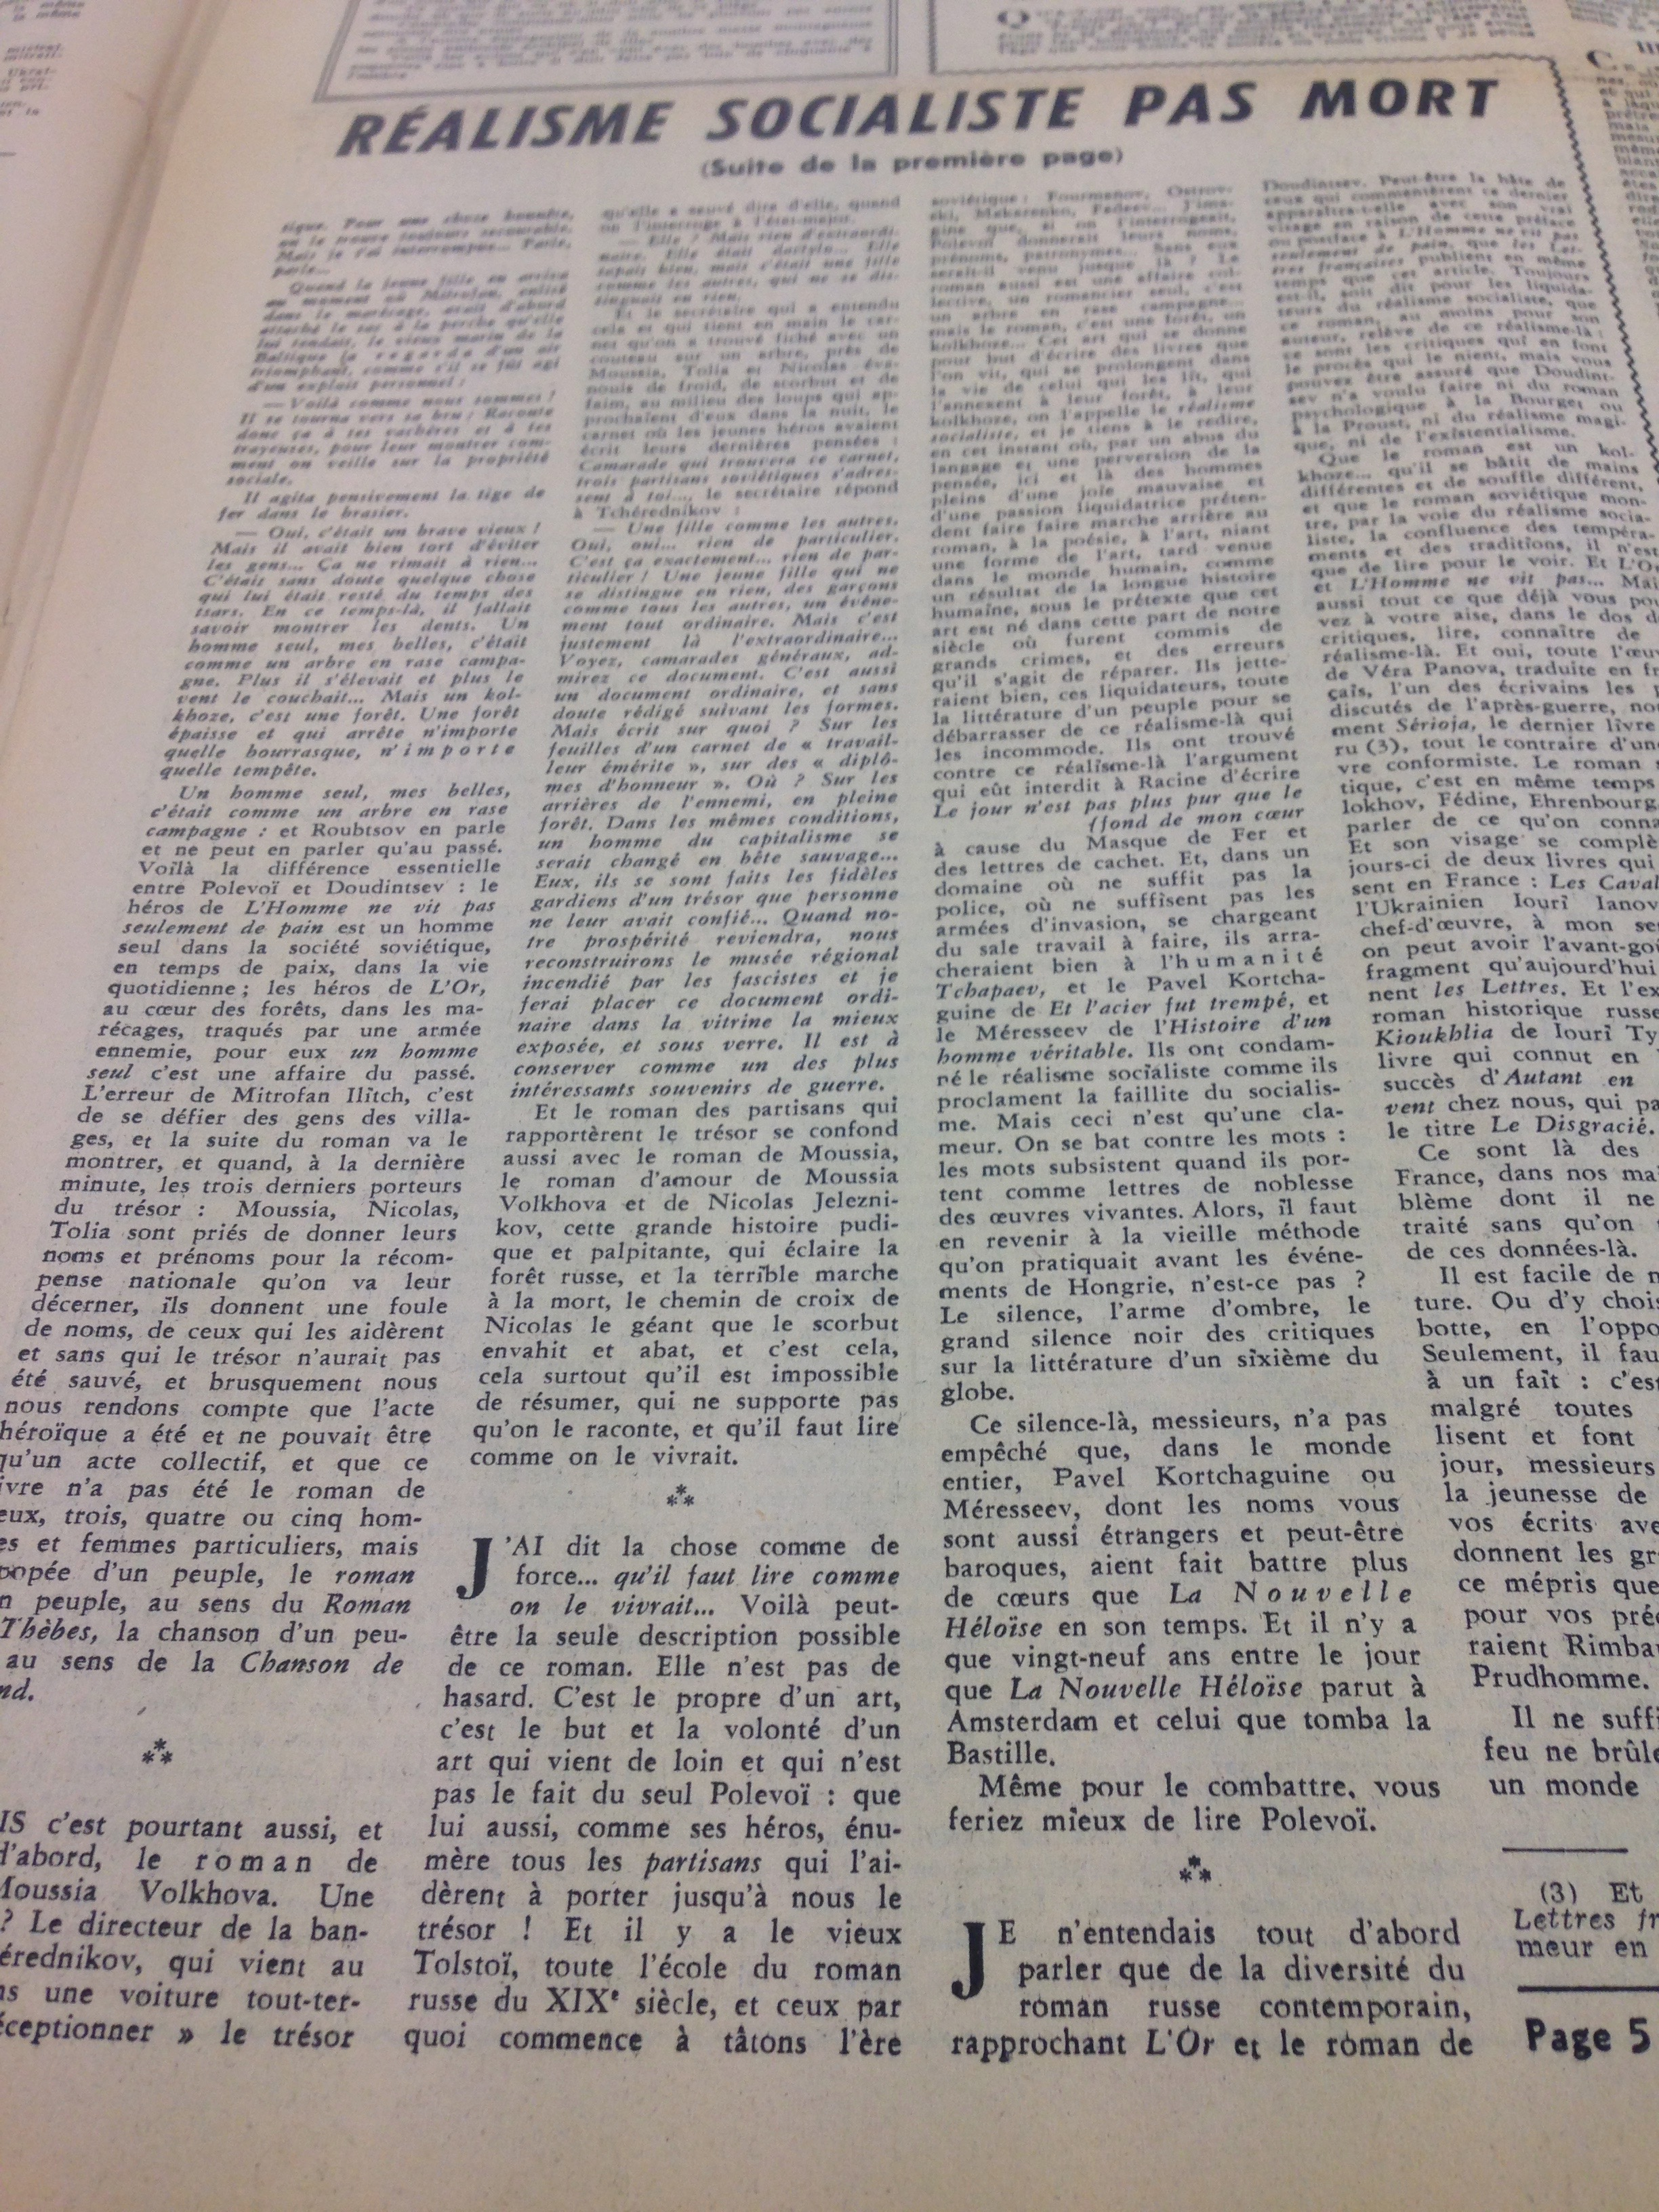
\includegraphics[width=0.33\textwidth]{realismesocialisten673.jpg}
	\caption{\cite{realsoc}}\label{fig:Réalistesocialistepasmort}
\end{figure}

	

	Or, comme dans beaucoup d’illustrations des \emph{Lettres françaises }lorsqu’il s’agit d’André Masson, c’est un dessin qui représente ses \oe{}uvres dans un numéro quelques mois plus tôt dans la rubrique \emph{A travers les galeries}\footcite{atraversgaleries}, par Pierre Descargues, illustré d'un Un dessin inachevé. On rejoint là encore, sur le plan artistique cette fois, une conception de la figuration étroitement liée à la politique communiste, et sur laquelle le réalisme socialiste peut en partie exercer une influence : celle de la préférence du dessin sur la peinture à l’huile. D’autant plus du dessin inachevé, plus proche encore de la genèse de l’oeuvre et du geste originel de l’artiste. 

\begin{figure}[H]
   \centering
   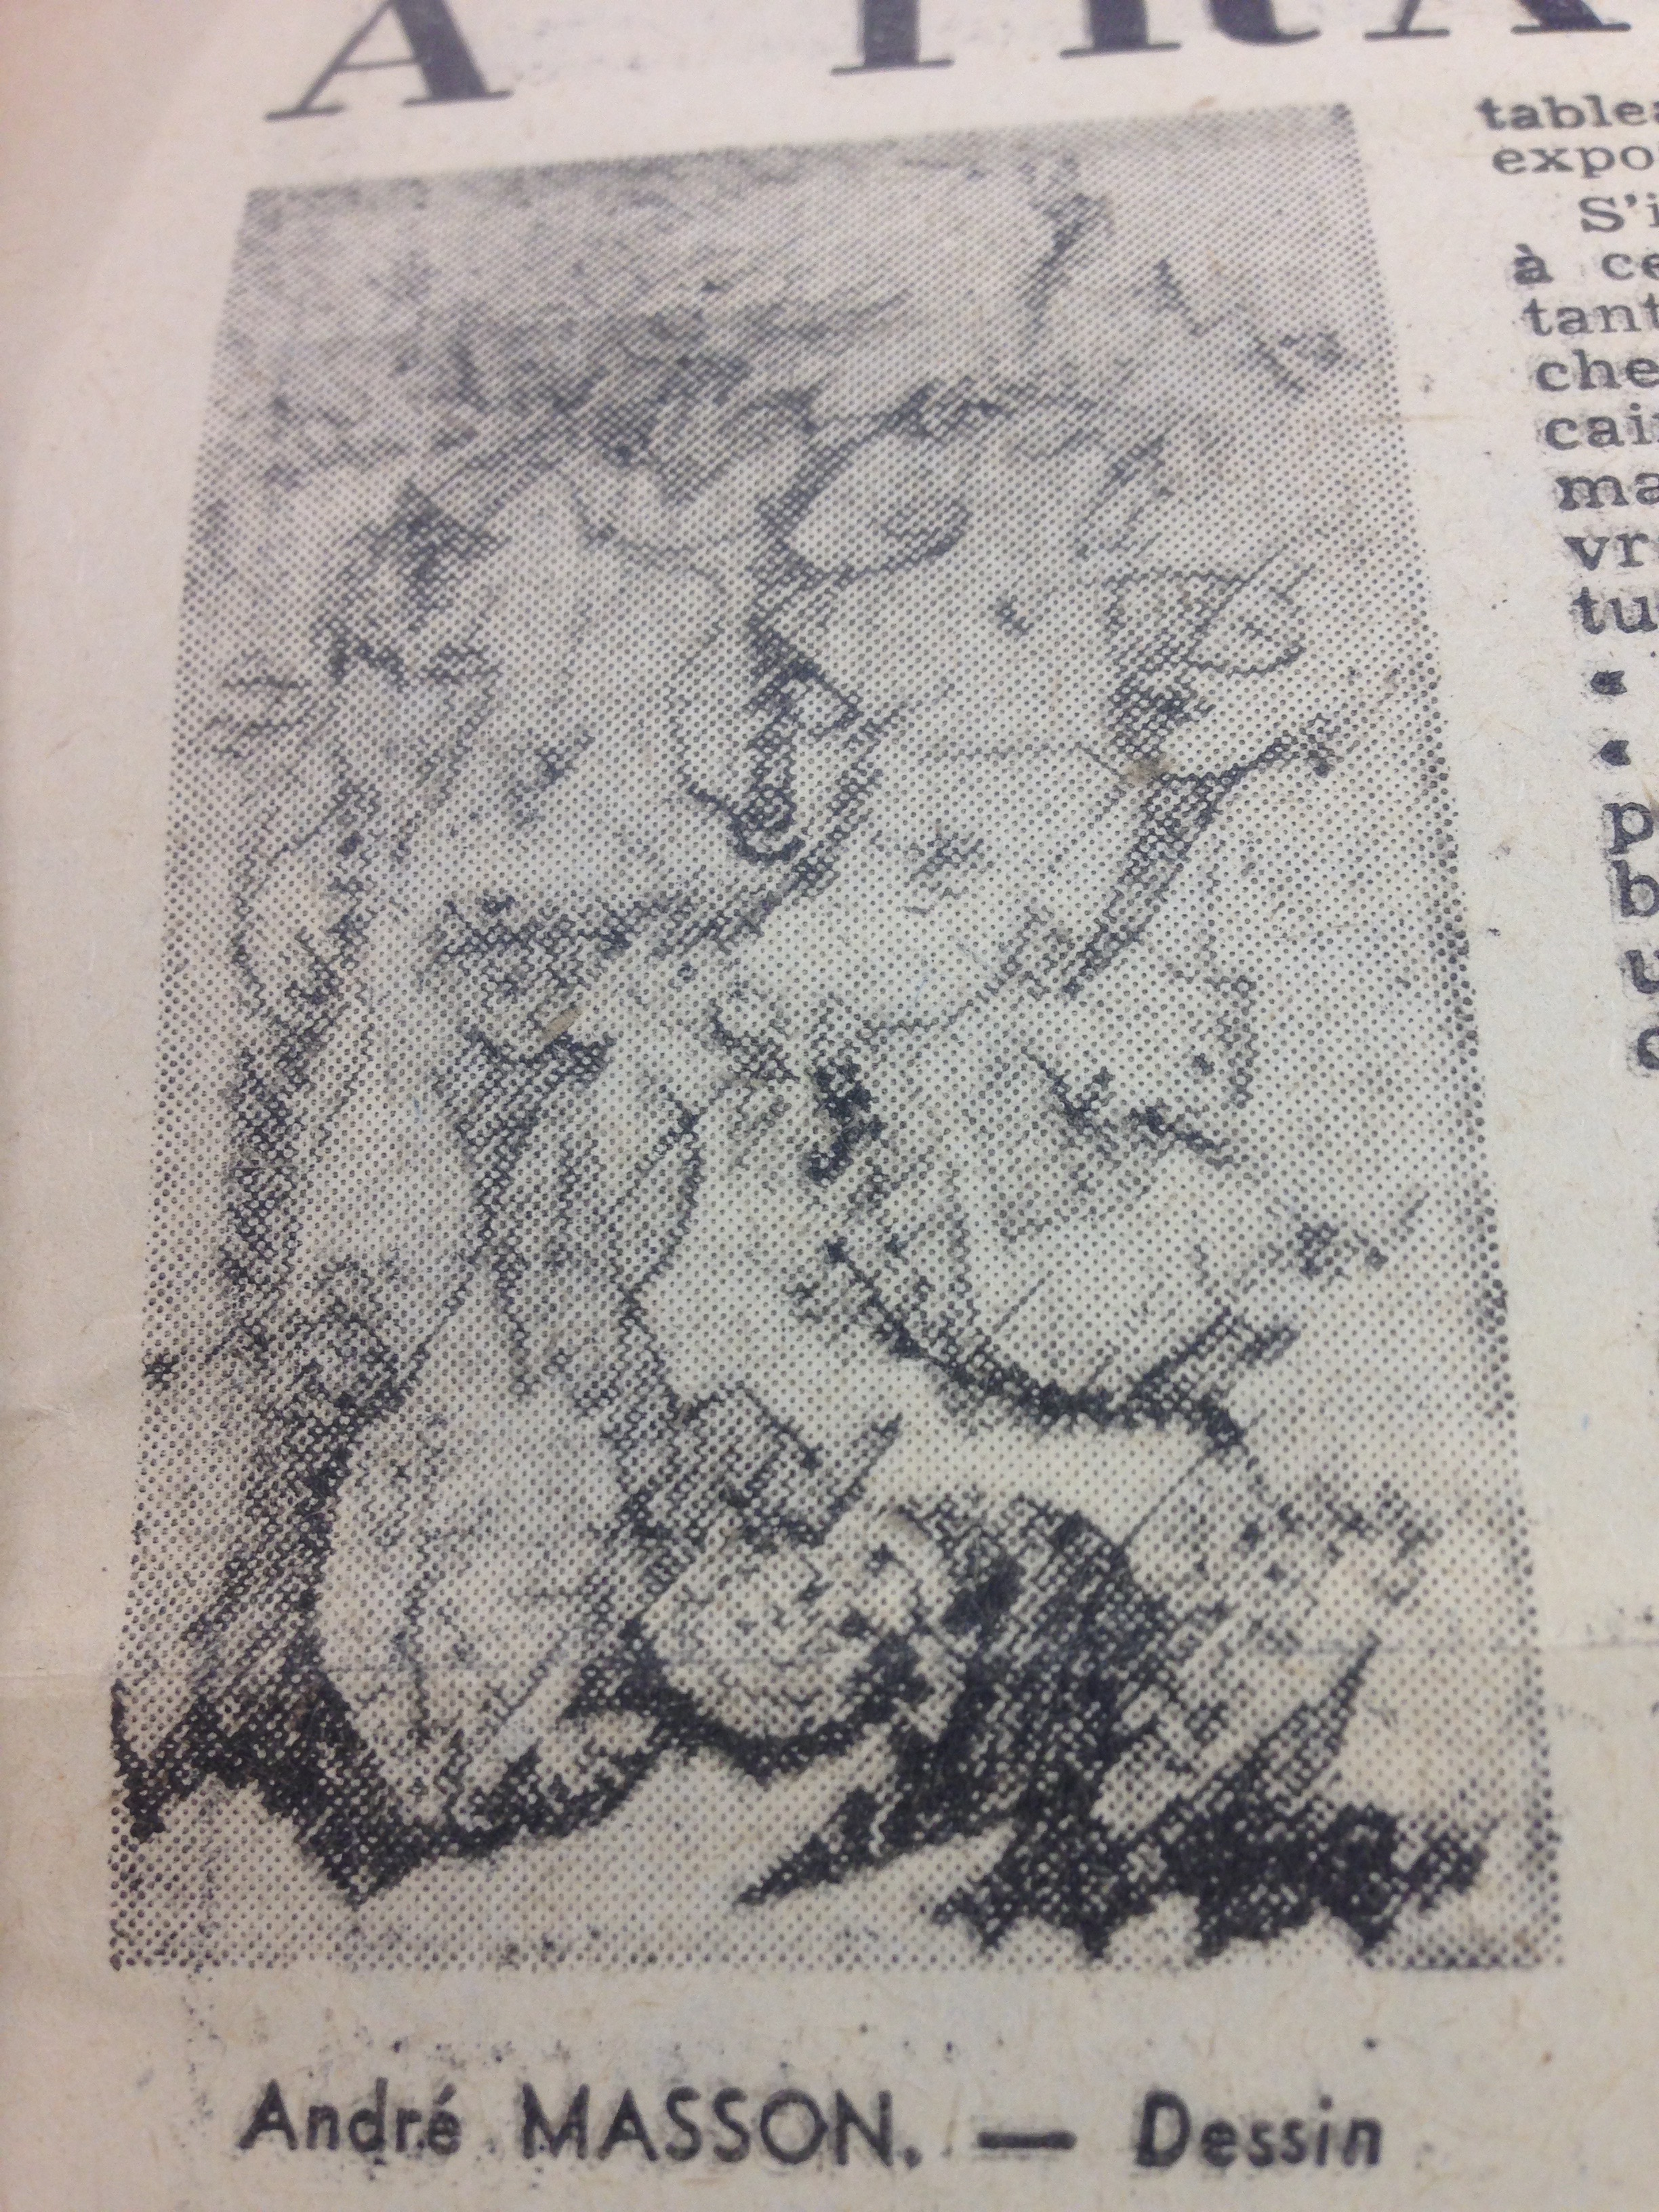
\includegraphics[width=0.33\textwidth]{dessingaleriesn669.jpg}
	\caption{\cite{realsoc}}\label{fig:Atraverslesgaleries}
\end{figure}



	Et pourtant, Masson peut-il être un représentant du réalisme socialiste ou de la politique du parti communiste, alors que sa figuration d’une réalité autre rend ambiguë la frontière entre la figuration et l’abstraction ? 
	
	\begin{quote}
	 Hors d’un trait nerveux, de rayonnements colorés, remarquables, vous ne reconnaîtrez pas Masson à son style. Ce peintre ne s’est pas laissé peindre à cette mode du graphisme en quoi l’on veut que chacun se résume. Il ne veut pas non plus être le peintre de quelques accords de couleurs. Si jamais artiste a fui le style, c’est bien lui. Aussi trouve-t-ton plus d’un tableau déconcertant dans cette exposition.\footcite{atraversgaleries}\end{quote}
	
	 Masson à contre-courant, donc. Le dessin au-dessus des lignes de la chronique n’est lui-même pas immédiatement identifiable, et c’est d’abord des figures abstraites qui apparaissent. Néanmoins, et c’est probablement en raison du choix de représenter une réalité autre, si le sujet n’est pas immédiatement identifié, il se devine. 

Il se devine par le biais de ce qui justement évoque dans un premier temps l’abstraction :les lignes, le tracé. Le corps d’une jeune femme nue en pleine nature apparaît dans les courbes des lignes. Une telle scène présenterait donc un sujet classique, mythologique ou sur la femme, deux thèmes chers à Masson, mais totalement redécouverts avec un nouveau regard de la part de l’observateur qui a deviné le sujet à la fois caché et révélé par le trait. Or, non seulement la figuration existe, mais puise son efficacité dans l’ambiguïté, mais il en de même pour le traitement des sujets : 

\begin{quote}
il s’attache à exprimer ces idées simples qui sont aussi des sensations et des spectacles d’une complexité formidable. Tant de choses tiennent-elles dans la peinture ? Il les y met, en tout cas, et trop souvent nous nous trouvions que devant un graphisme nerveux, devant quelques virgules nageant dans la couleur, devant de puissants mouvements.\footcite{atraversgaleries}\end{quote}

 
	On remarque d’ailleurs que les deux aspects sont tout autant des compliments pour Pierre Descargues : d’une part, la \enquote{simplicité}, avec des sujets au titre très bref généralement sur un sentiment, un personnage de mythologie, les femmes, les scènes de massacres. D’autre part, \enquote{des spectacles d’une complexité formidable}. Masson rechercherait-il avec une autre forme du réel une autre représentation du sublime ?  Or, si l’on regarde le dessin publié au-dessus de l’article, la simplicité apparente s’accompagne si l’on suite les traits jaillis du corps féminin une grande part de détails : la courbe de la tête de la femme penchée, les motifs autour d’elle et à ses pieds. Des personnages inachevés surgissent même dans les airs. Ils surgissent parce qu’on ne les distingue pas tout de suite, et l’on ne sait pas immédiatement s’ils sont produits par l’hallucination du spectateur ou bien réellement produits par fragments par le mouvement des traits. 

	Avec cette création de personnages, les lignes ne composent pas uniquement le sujet, mais le racontent, mais comme le ferait non pas un narrateur mais plusieurs, plus proches de la polyphonie due à des voix mélangées. Il peut ainsi paraitre paradoxal qu’à l’heure du réalisme socialiste, ce dessin, certes pleinement représentatif du geste du dessinateur en train de créer comme l’apprécie le communisme, se rapproche plutôt du dessin automatique conçu par les surréalistes. On peut se demander devant ce dessin d’André Masson si le sujet de cette jeune femme nue était réfléchi avant le geste du dessin, ou si c’est justement l’inconscient des traits qui ont formé le sujet. La référence de Descargues au traitement de la couleur est intéressante, puisque le choix du dessin justement privilégie la forme, les fameuses \enquote{quelques virgules nageant dans la couleur}. Les couleurs du dessin révèleraient-elles alors une toute autre \oe{}uvre ? Or, les couleurs sont ancrées elle-mêmes dans le tourbillon de la forme, indissociables du mouvement. Ce qui justifie le choix des \emph{Lettres françaises}, fait pour beaucoup d’artistes, mais particulièrement pour André Masson, de privilégier ses dessins et esquisses aux tableaux : le mouvement figure à la fois le tracé et la couleur. Il est la composition dans sa totalité. Pour autant, pourquoi André Masson n’incarne-t-il pas  la ligne du réalisme socialiste ? 


On se rappelle qu’en 1952, Aragon précise dans son article sur le prix Staline décerné au \emph{Premier Choc} d’André Stil non seulement la définition du réalisme socialiste, mais aussi que celui-ci peut évoquer la peinture en parlant d’un livre et réciproquement. Or, dans l’article \emph{Réalisme socialiste pas mort} de 1957, Aragon commente deux oeuvres littéraires avec une distinction sur leur vocation romanesque : \enquote{Cela dit, il y a deux sortes de romans : ceux qui se racontent, comme celui de Doudintsev (2); ce dont on ne peut dire que le thème, comme celui de Polevoï}. Cette distinction est intéressante au regard des oeuvres de Masson, dont le titre désignerait plutôt un thème. Pourtant, si l'on regarde la scène fantastique de la femme nue dans la nature du \emph{Dessin }publié pour la rubrique \emph{ÀTravers les galeries}quelques semaines plus tôt, peut-on être sûr que les traits ne racontent rien ? 

	Les traits vifs racontent avant même le sujet quelque chose de l’état d’André Masson en train de dessiner. Si narration il y a, elle n’est ni réfléchie ni anticipée, pour privilégier au contraire la vitesse du geste de création. D’après Bernard Noël, à propos des dessins automatiques de Masson, la vitesse c’est à la fois ce qui fait de Masson une figure emblématique du dessin automatique, tout en le mettant à part des autres artistes surréalistes : \enquote{Cette vitesse-là- celle même de l’automatisme - fait bien d’André Masson le premier peintre surréaliste, et cependant elle travaille à l’éloigner du groupe parce que l’explosante en elle-même n’est jamais fixe.} Ainsi, même avec l’empreinte indélébile du surréalisme dans ce Dessin, André Masson est à la fois une figure d’autorité sans pour autant être un modèle, puisque son style n’est pas suivi même pas les auteurs de dessins automatiques de sa génération. 

	Mais, en 1957, présenter ce \emph{Dessin} révélateur du tracé originel est sans doute la seule caractéristique commune entre André Masson et un réalisme socialiste qui n’est plus en plein essor en 1952 mais plutôt au stade de survie, comme l’induit le titre \emph{Réalisme socialiste pas mort}. Le lyrisme est cependant de première importance aussi bien dans ce \emph{Dessin} de Masson que dans ces critiques de livres réalistes socialistes par Aragon. Mais la différence notable de l’expression lyrique tient probablement au rapport avec le temps : André Masson exprime des émotions dans l’instantanéité de l’instant présent. Le sujet, cette jeune femme n’existe en tant que telle que parce que dessinée dans la vitesse du temps présent. La mobilité de son corps en témoigne, et pas un élément même parmi les personnages inachevés ou apparement naturels n’est statique. Or, la critique littéraire des oeuvres soviétiques réalistes socialistes par Aragon ne crée pas le lyrisme par le mouvement vif du présent, mais par la nostalgie, le passé : 

\begin{quote}
…c’est la donnée initiale du livre, mais comment suivre le détaille leurs aventures, restituer le tragique de cette histoire, rendre le parfum de la terre russe, de ses forêts dans l’été de 1941, le paysage bouleversant et boulversé, les passages d’hommes et d’animaux sur les pistes secrètes à deux pas de l’armée d’invasion en marche ?\footcite{realsoc}\end{quote}	


Le fait que cette nostalgie soit vouée à l’URSS n’est sûrement pas anodin, et l’on pourrait presque entendre dans ce romantisme des lieux russes la propre nostalgie d’Aragon pour le pays dans son poème \emph{Hourra l’Oural} de 1934 : \enquote{C’est troublant / c’est tout à fait tremblant / Simplement sous leurs pieds la terre /s’était mise à se souvenir / L’Oural rêvait}\footcite{hourra}. Comme dans la critique du livre \emph{L’Or de Polevoï}, le lyrisme se construit autour de la terre, le symbole d’un lieu natal mais qui est aussi un espace ancré, fixe, là où les traits de Masson ne cherchent pas à retrouver le passé sacralisé. Le visage du couple, d’une femme est chez Polevoï comme dans \emph{Hourra l’Oural} mêlé aux racines russes, ce qui renforce l’imaginaire romantique autour de la terre natale, ou symboliquement natale dans le cas d’Aragon. Le trait de Masson, lui, est en partie éphémère, avec ses personnages inachevés, sans origine distincte puisque le tracé est emmêlé. Ainsi, si le lyrisme est omniprésent dans le \emph{Dessin} comme dans la critique d’oeuvres réalistes socialistes, son traitement est nuancé.
%reprebdre p 102- (p16) 


	D’autre part, la critique d’Aragon repose sur la nécessité d’un héros collectif et réhabilite le genre noble par excellence, l’épique : 
	\begin{quote}
	et brusquement nous nous rendons compte que l’acte héroïque a été et ne pouvait être qu’un acte collectif, et que ce livre n’a pas été le roman de deux, trois, quatre ou cinq hommes et femmes particuliers, mais l’épopée d’un peuple, le roman d’un peuple, au sens du \emph{Roman de Thèbes}, la \emph{Chanson de Roland}.\footcite{realsoc}\end{quote}
	
	
	 Or, si l’épique est d’une part un genre peu présent dans la production littéraire contemporaine, c’est aussi pour Aragon en tant que directeur des \emph{Lettres françaises} de faire du réalisme socialisme un aboutissement à la Résistance, l’origine de la création du journal. 

	André Masson n’est pas étranger à l’expression de l’acte de résistance, mais la création ne peut pas venir du collectif, mais au contraire d’un point de vue intime, puisque la liberté des traits du dessin vient de la notion de désir. C’est pourquoi la liberté est polyphonique dans les oeuvres de Masson : Libertaire comme dans ce \emph{Dessin}, et l’expression appuyée du corps féminin nu et la retranscription en mouvement d’un autre type de cri qui est celui de la révolte. Mais la nature même du dessin automatique et sa remontée vers l’inconscient ne permet pas de reposer sur une dimension collective propre au réalisme socialiste. Cependant, d’un point de vue intime ou collectif, André Masson comme le réalisme socialiste cherchent à retranscrire le ressenti du peuple avant même sa représentation. 

	C’est pourquoi la finalité réclamée par Aragon dans les dernières lignes de sa critique littéraire rejoint celle du Dessin d’André Masson et sa figuration comme ressenti du réel, et non plus son mimétisme : 

\begin{quote}
Un jour, messieurs les liquidateurs, la jeunesse de ce pays déchirera vos écrits avec ce mépris que donnent les grands enthousiasmes, ce mépris que ma génération eut pour vos prédécesseurs qui ignoraient Rimbaud au nom de Sully Prudhomme.\footcite{realsoc}\end{quote}
 
	 En réactivant la vieille querelle de Rimbaud contre les Parnassiens, Aragon sous-entend que le réalisme socialiste est méprisé, du moins en partie en France, pour d’autres courants littéraires privilégiés qui occupent le devant de la scène. Mais on retrouve aussi dans cette défense du réalisme socialiste les prémices de la thèse défendue en 1959 dans \emph{Savoir aime}r à propos du travail de critique : Le réalisme socialiste a pour essence l’\enquote{enthousiasme}, autrement dit ce qu’Aragon exige aussi de la critique en général.  

	Or, avec son exigence de vitesse lorsqu’il dessine, André Masson recherche lui aussi un jaillissement de l’expression au sens le plus vif. Cet élément qui est sans doute l’élément le plus fondamental du texte est aussi le plus intimement proche de l’esthétique d’André Masson : \enquote{Il ne suffit pas de dire que le feu ne brûle pas quand c’est tout un monde qui s’embrase}. Cette phrase au présent gnomique aux allures de maxime est celle mise à part des autres et qui conclut l’article. Même si la passion qu’Aragon évoque comprend avec le \enquote{monde} la dimension collective théorisée précédemment, le lieu commun des flammes rejoint les métaphores astrales de Masson permanentes dans ses écrits : Si le réalisme socialise exige une forme collective, basée sur la tradition épique mais aussi plus onirique avec la référence aux troubadours et à la performance, le lien étroit entre le concept et l’art de Masson se fait au niveau d’une réception aux attentes analogues : Une certaine dévastation est attendue, un dérèglement des sens. Le lecteur d’une oeuvre réaliste socialiste et un spectateur d’une oeuvre de Masson doivent être à l’inverse de la passivité, ou de toute distanciation. 

	On peut d’ailleurs soupçonner Masson en dessinant à partir de l’intime pour produire ce mouvement conçu à partir de flux de pensées de parler en réalité non d’un homme mais de l’homme. Or, cette passion qui répond à deux projets différents mais qui est nécessaire dans la création répond aux mêmes exigences en terme de réception, et rejoint ainsi une conception spécifique de l’homme. L’image de la flamme est aussi et surtout le lieu commun du désir. Le désir est aussi l’essence même de la création de Masson. 

C’est pourquoi il ne s’agit pas en convoquant ces notions de soulèvement de passion de confondre l’art d’André Masson caractérisé par ce \emph{Dessin} dans l’idée que proclame Aragon sur le réalisme socialiste. D’abord, comme la négation à la tête du titre l’évoque, \emph{Non le réalisme socialisme n’est pas mort}, Aragon est dans une position de défense et de refus. On comprend d’ailleurs quel facteur décisif peut être l’appel aux passions pour justifier la continuité de son existence malgré cette période obscure pour le réalisme socialiste après le rapport de Khrouchtchev le 24 février 1956 où les crimes et déportations de Staline sont dénoncés pendant ce XXème Congrès de Moscou. Pourtant, les deux événéments que sont les ouvrages exaltés par Aragon rappellent aussi le synonyme que l'écrivain prête à la valeur \enquote{réaliste socialiste} :  

\begin{quote}
\enquote{la récompense du réalisme}, a depuis longtemps trouvé son fondement doctrinal dans le romantisme révolutionnaire, l'autre nom, on le sait, du réalisme socialiste.\footcite[p1012]{these}\end{quote}

Les termes mêems de cette autre désignation induisent immédiétement tout un panel d'affects qui expliquent quel déchirement interieur signfierait pour Aragon de renoncer au \enquote{réalisme socialiste}. Le réalisme socialiste est ainsi désigné sous son autre nom comme le lieu des passions par excellence et sous-entend sa visée utopique. 

% Voir Chronique du Bel Canto. (Fait)

	 Ainsi, en concluant par cette métaphore du désir, Aragon ne mentionne plus la passion autour du stalinisme, présente dans sa définition de 1952 lors de la remise du Prix Staline à André Stil. En revanche, il préserve une substance idéologique indépendante de la figure de Staline. Or, si l’on compare l’image de l’homme selon Aragon au nom de ce réalisme socialiste revisité et celui d’André Masson où du désir s’exprime une vision de l’homme, sur l’homme, on voit que de ces deux désirs aboutissent une conception idéologique proche et intime. Il n’est pas certain que les autres auteurs réalistes socialistes ou les dirigeants et militants communistes approuvent totalement la réorientation du réalisme socialiste d’Aragon, forcément plus personnelle à présent, et que ce socialisme se rapproche de la vision socialiste aussi d’André Masson sur les hommes. C’est pourquoi on peut se demander si l’origine de cette perception idéologique, créative et réceptive n’est pas due à cette conviction essentielle chez les deux hommes que l’idéologie politique naitrait de leur création, \enquote{et non pas l’inverse}\footcite{}. 
%Source web : 	http://fresques.ina.fr/jalons/fiche-media/InaEdu01226/louis-aragon.html : Aragon assit autour d’étudiants le 27 janvier 1967. (Fait)

\section{Discours récurrents des \emph{Lettres françaises} autour d’André Masson (n1104- du 4 au 10 novembre 1965)}  

\subsection{Numéro des \emph{Lettres françaises} : André Masson et le Plafond de l'Odéon }


Le journal \emph{Les Lettres françaises}, qui se compose à partir d’un fil conducteur sur des thèmes spécifiques dans chaque numéro, s’arrête nécessairement sur les éléments de l’esthétique d’André Masson.  Ils font corps avec l’idée-phare du numéro.  La récurrence de topoï dans les discours des journalistes et des années pour qualifier l’art d’André Masson sert ce dessein éditorial. L’esthétique de Masson va être associée grâce aux discours des chroniqueurs à l’idéologie politique du journal. Le rapport d’André Masson aux \emph{Lettres Françaises} est aussi profond que multiple : D’abord comme grand lecteur lors de son exil aux Etats-Unis : 

\begin{quote}
Votre lettre m’a fait le plus grand plaisir. Je vous prie de m’excuser : j’ai tant tardé à vous écrire que je recevais les “lettres Françaises“ (la seule revue à cette heure qui nous rappelle que quelque fois les Français savent penser et écrire) », « « J’ai lu votre très beau texte : “La Pampa“ dans le dernier numéro que j’ai reçu des L.F- Si cette revue ne paraît plus ce sera désolant. (Lettres françaises, n\degre 4, 1er avril 1942, pp. 1-3).\footcite[p478]{anneessurrealistes}
\end{quote}
 

	Ainsi, \emph{Les Lettres françaises }figurent pour l’artiste le dernier moyen d’avoir encore foi en l’humanisme. Cette réception n’est donc pas anodine, surtout à la lumière des articles de grands chroniqueurs du journal lorsque ces derniers même une vingtaine d’année plus tard parleront de Masson. De même, cette réception très forte chez Masson et qui voit en ce journal le dernier rempart de la pensée peut-être une expérience déterminante lorsque lui-même écrit un article pour \emph{Les Lettres françaises}, ce qui arrive dès les années 50. Plus précisément, les articles de Masson, dont une qualité littéraire est reconnue par le journal lui-même en plus de son immense culture, ont pour vocation généralement la revendication d’une certaine vision de l’art. Ce travail dans les analyses de Masson passe généralement à travers la figure d’artistes comme Turner, Cézanne. La figure de Cézanne en particulier dépasse l’hommage, le journal même une dizaine d’années plus tard, composera tout un engagement pour sauvegarder la mémoire de l’artiste, oubliée dans sa région d’origine. 

On touche déjà à des questions qui relèvent de choix d’engagements politiques du journal. Sans compter les grandes enquêtes dont la problématique est centrée sur l’art dans plusieurs numéros. Masson y apparait comme l’un des discrets mais toujours fidèles intervenants. Or, il va s’agir de constater à quel point l’esthétique d’André Masson va poursuivre un fil conducteur extérieur à son oeuvre, l’idéologie de la politique éditoriale des Lettres françaises. C’est pourquoi nous pouvons d’abord nous pencher sur ces topoï récurrents, pour ne pas dire persistants, qu’auront les journalistes des \emph{Lettres françaises} vis-à-vis d’André Masson. D’autant plus que la plupart de ces journalistes précisent bien le connaître personnellement, ce qui inclut l’aspect individuel, humain de l’artiste dans leur analyse de l’art d’André Masson. 

	A ce titre, le numéro sur le plafond de Masson pour le théâtre de l’Odéon est particulièrement révélateur. Il comprend non seulement l’article de Georges Boudaille, mais aussi les notes d’André Masson sur ce même sujet. D’autant plus que les deux articles co-existent sur la même page, à la suite des esquisses du plafond. Leur titre, \emph{Les premières esquisses d’André Masson} se prolonge naturellement avec l’article \emph{Notes de travail d’André Masson} par leur valeur commune d’état naissant. 

	\begin{figure}[H]
   \centering
   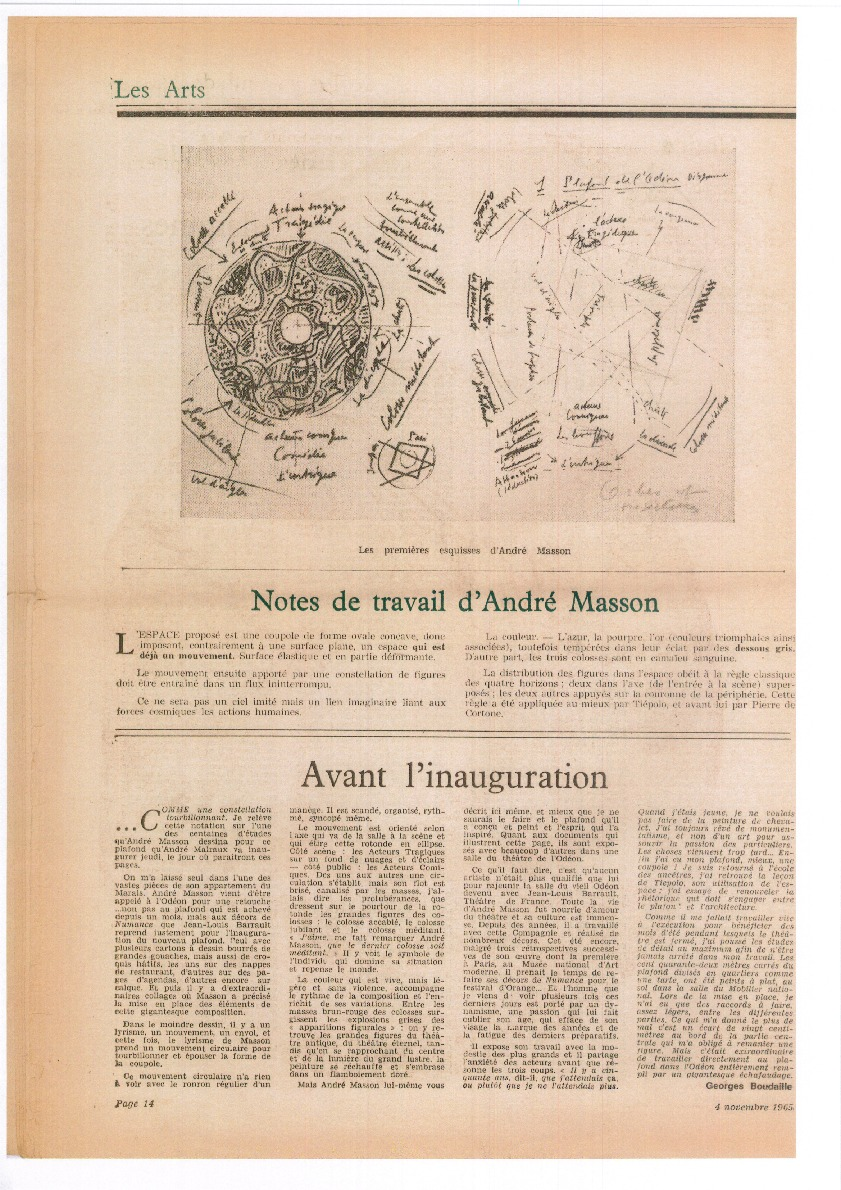
\includegraphics[width=0.33\textwidth]{massonesquissesplafond.jpg}
	\caption{\cite{plafondodeon}}\label{fig:Notesdetravail}
\end{figure}



Même l’article de Georges Boudaille,\emph{Avant l’inauguration}\footcite{avantinauguration}, joue sur une forme de genèse. \emph{Ces notes de travail d’André Masson}, citées au centre de la page comme le point fixe d’une image, accrochent particulièrement le regard avec le choix éditorial de colorer le titre en vert, de même que la banderole autour du titre des \emph{Lettres françaises}. Reste à savoir si les fragments mis en gras plutôt que d’autres respectent une différence de marque typographique des notes originelles de Masson, ou si le numéro a voulu accentuer la réflexion de Masson sur son travail en extrayant des notions-phares dans le texte. L’importance de cette distinction typographique n’est pas moindre, d’abord pour le choix de colorer le titre de cet article et des termes extraits en gras, si l’on prend en considération l’enjeu majeur qu’en fait Aragon en tant que directeur de journal: 

\begin{quote}
L’abondance de ces variations graphiques, sur lesquelles Aragon a veillé, témoigne de son intérêt de grand directeur de journal pour la dimension matérielle du livre et les effets signifiants qui en découlent. On sait le lien d’Aragon avec les typographes des Lettres françaises et de nombreuses photos le montrent travaillant avec eux au marbre du journal.\footcite[p333]{vasseviere}	
\end{quote}

	 Or, dans le cas de ces deux extraits mis en gras dans l'article, ce sont les caractéristiques de l’espace et de la couleur qui percutent l’oeil du lecteur avant même la lecture des notes. Ainsi ces deux fragments précisément mis en gras : \enquote{qui est déjà un mouvement} à propos de l’espace oval du plafond, et  les \enquote{dessous gris} pour tempérer la vivacité des couleurs rouge et or, rejoignent la valeur signifiante évoquée par Maryse Vassevière. En outre, le premier fragment est révélateur non seulement d’une caractéristique essentielle dans l’esthétique d’André Masson, peut-être même sa principale, mais aussi d’un topos récurrent chez les critiques pour qualifier Masson : \enquote{qui est déjà un mouvement}. Sous-entendu, avec l’adverbe \enquote{déjà}, que la forme ovale anticipe le désir créateur de Masson de créer le mouvement dans l’espace. Et, comme par un jeu de dialogue interne ininterrompu, signifié par les points de suspension à l’ouverture de l’article, facilité par la proximité de ces articles voisins, Georges Boudaille entame son propre article avec d’autres termes de Masson. Ils reprennent cette exigence fondamentale que doit être le mouvement:\enquote{\emph{Comme une constellation tourbillonnant}}.  On remarque la portée dévastatrice que suggère la métaphore du tourbillon. 

	En outre, il  ressort de cette combinaison de la \enquote{constellation} et du tourbillon la volonté de prévaloir dans son langage la fonction poétique : Une écriture, pourtant à l’état de \enquote{notes}, et que l’on attendrait par conséquent plutôt résiduelle, schématique. C’est d’ailleurs bel et bien le mouvement qui fascine Georges Boudaille chez André Masson, comme l’illustre la gradation ascendante des quelques lignes de ce paragraphe : \enquote{Dans le moindre dessin, il y a un lyrisme, un mouvement, un envol, et cette fois, le lyrisme de Masson prend un mouvement circulaire pour tourbillonner et épouser la forme de la coupole}. 

	Ainsi, la forme ovale, en rencontrant les formes elles-mêmes agitées de Masson ne crée pas seulement ce mouvement qui existe \enquote{déjà}, mais provoque en revanche ce tourbillon induit dans la citation que Boudaille extrait des notes de Masson et qui reparait dans sa propre écriture. Cette image du tourbillon induit une idée de force de cet élément naturel dans le paragraphe suivant, axé lui aussi sur le mouvement : \enquote{Ce mouvement circulaire n’a rien à voir avec le ronron régulier d’un manège. Il est scandé, organisé, rythmé, syncopé même}. En somme, le contraire de la monotonie, et l’agitation réfléchie, puisque André Masson en organisant le mouvement travaille surtout à l’orientation, circulaire aussi, du regard : \enquote{“\emph{J’aime, me fait remarquer André Masson, que le dernier colosse soit méditant“}. Il y voit le symbole de l’individu qui domine sa situation et repense le monde.} Ainsi, la notion fondamentale du mouvement dans une esthétique aussi difficilement identifiable d’une oeuvre à l’autre chez Masson, comme ne le manqueront pas de le souligner dans d’autres numéros les critiques, comprend lui-mêmes deux valeurs essentielles dans sa création : Le lyrisme syncopé à l’agitation, et sa finalité tournée vers l’homme. 

	En somme, un portrait d’une idée de l’homme figuré par le mouvement, comme le sous-entend au plafond de l’Odéon la fin du cercle sur la figure du penseur. Le mouvement d’André Masson ne se limite donc pas à la question esthétique, puisque toute l’organisation de celui-ci suit un fil humaniste, dans cet exemple du plafond de l’Odéon : \enquote{Ce ne sera pas un ciel imité mais un lien imaginaire liant aux forces cosmiques les actions humaines}, mettent en garde ses \emph{Notes de travail} dans l’article précédent. Cette orientation se rapproche d’un idéal, lorsqu’on se rappelle de la désolation d’André Masson pendant la 2nd Guerre Mondiale, où, depuis les Etats-Unis, la seule trace de pensée en Europe résidait dans la revue \emph{Les Lettres françaises}. Masson établit donc un portrait de l’homme par le mouvement puisqu’il ne peut concevoir celui-ci qu’à travers sa faculté de penser. 

En outre, l’article de Georges Boudaille respecte la structure de l'article  \emph{Notes de travail d’André Masson} qui précèdent son article, puisque qu’après l’analyse du mouvement chez Masson, Boudaille évoque la couleur : \enquote{La couleur qui est vive, mais légère et sans violence, accompagne le rythme de la composition et l’enrichit de ses variations}. 

	On reconnait dans cette description la tempérance du rouge et de l’or permise par les \emph{dessous gris}, l’autre fragment en gras dans le texte. D’autre part, cette description sur la combinaison de couleurs vives sur un fond tempéré évoque tant chez Masson que chez Boudaille le principe de la devise : \enquote{La couleur . — L’azur, le pourpre, l’or (couleurs triomphales ainsi associées), toutefois tempérées dans leur éclat par des \textbf{dessous gris.}}L’agitation des couleurs maitrisées par la tempérance, une forme de raisonnement. La réflexion des couleurs, tout aussi minutieusement détaillée bien que n’étant pas visible dans les esquisses du numéro, est finalement fondée exactement sur le même raisonnement que pour la forme du mouvement : L’éclatement doit apparaitre avec la même énergie que le mouvement des personnages, éclater au regard, mais le lyrisme n’est possible qu’avec l’harmonie de ses couleurs vives avec le fond gris.


	C’est pourquoi il ne s’agit pas tant en soit de limiter l’agitation de la ronde que l’orienter vers un idéal de la Pensée, c’est-à-dire la faculté de l’homme à perpétuellement penser, avec ses forces et ses contradictions, mais dans une finalité humaniste, donc maitrisée. On pourrait presque remplacer \enquote{peinture} par \enquote{pensée} lorsque Boudaille conclut ainsi son paragraphe sur la couleur : \enquote{tandis qu’en se rapprochant du centre et de la lumière du grand lustre, la peinture se réchauffe et s’embrase dans un flamboiement doré.}  On trouve ici une idée d’apothéose, qui n’est pas sans rappeler l’esthétique sublime du XVIèmme avec la dimension spectaculaire qu’elle comporte. L’apothéose de la pensée passe également par l’organisation lorsque Masson choisit d’arrêter le regard avec pour dernier personnage l’homme qui médite : Il signifie le mouvement de la pensée par excellence. 


En outre, Georges Boudaille use de cette force du mouvement comme tourbillonnons seulement pour analyser les dessins et le plafond de l’Odéon d’André Masson, mais également pour décrire comment cette force rejaillit sur l’artiste : \enquote{aucun artiste n’était plus qualifié que lui pour rajeunir le théâtre du vieil Odéon}, \enquote{Et l’homme que je viens de voir plusieurs fois ces derniers jours est porté par un dynamisme, une passion qui lui fait oublier son âge, qui efface de son visage la marque des années et la fatigue des derniers préparatifs.}. Ainsi, par jeux de reflets, l’art basé sur le mouvement influence l’individu, et non l’inverse. 

	C’est grâce au dynamise recherché dans son oeuvre qu’André Masson en tant qu’individu devient lui-même un être en mouvement, jeune, c’est-à-dire ici perpétuellement vivant. C’est d’ailleurs avant de rapporter le discours de Masson pour conclure sa critique, de même qu’il l’avait débutée avec des mots de l’artiste, Boudaille le compare à une autre branche artistique, un comédien : \enquote{Il expose son travail avec la modestie des plus grands et il partage l’anxiété des acteurs avant que résonne les trois coups} : Cette théâtralité dans l’écriture de Boudaille lie cette valeur de la jeunesse attribuée à André Masson à une certaine forme d’innocence, une tempérance qui ne peut qu’évoquer les \enquote{dessous gris}, cette sagesse, qu’il recommandait à ses couleurs vives. Dans ses paroles rapportées, André Mason mêle d’ailleurs la rigueur exigée pour travailler sur le plafond, « j’ai poussé les études de détail au maximum afin de n’être jamais arrêté dans mon travail » à une forme d’extase procurée par son art, \enquote{Mais c’était extraordinaire de travailler directement au plafond dans l’Odéon entièrement rempli par un gigantesque échafaudage.}

	Ainsi, à l’image d’une devise, cette agitation raisonnée provoque un écho entre les \emph{Notes de travail d’André Masson} et la critique de Boudaille, elle-même largement partagée entre l’analyse de Boudaille et les paroles rapportées de Masson. Mais ce \enquote{mouvement perpétuel} qui figure l’homme en tant que penseur ne peut que sous-entendre une idéologie politique dans sa démarche esthétique et se rapprocher des problématiques d’Aragon. En particulier autour du devenir du réalisme socialiste. Les marques typographiques, discrètes mais tout de mêmes immédiatement visibles avant la lecture, dont les marques éditoriales distinguent un choix de mots très précis, ne peut que le rappeler. 


	Cette caractéristique principale du mouvement, qui est peut-être paradoxalement l’élément qui rend les oeuvres de Masson atypiques les unes aux autres (comment reconnaitre immédiatement une oeuvre d’André Masson que l’on a jamais vu ?), les journalistes des Lettres françaises ne se contentent pas de la souligner. 

	\subsection{Article \emph{André Masson à Lyon} par Gérard Guillot }

 Nous avons vu les valeurs idéologiques que suggéraient d’après ses esquisses sur le plafond de l’Odéon celles du numéro de Novembre 1965\footcite{sivous}. On peut à présent étudier quel autre axe idéologique cette esthétique du mouvement est analysée en Juillet 1967, à l’occasion d’une exposition d’André Masson à Lyon. Dans son article \emph{André Masson à Lyon}\footcite{massonlyon}, Gérard Guillot fait de ce mouvement un signe de liberté : \enquote{il faut aller à la rencontre d’André Masson au musée de Lyon; il faut aller dialoguer avec ses toiles et respirer leur grand souffle de liberté, celle de l’esprit, du coeur, des mouvements et des sens !}. 

\begin{figure}[H]
   \centering
   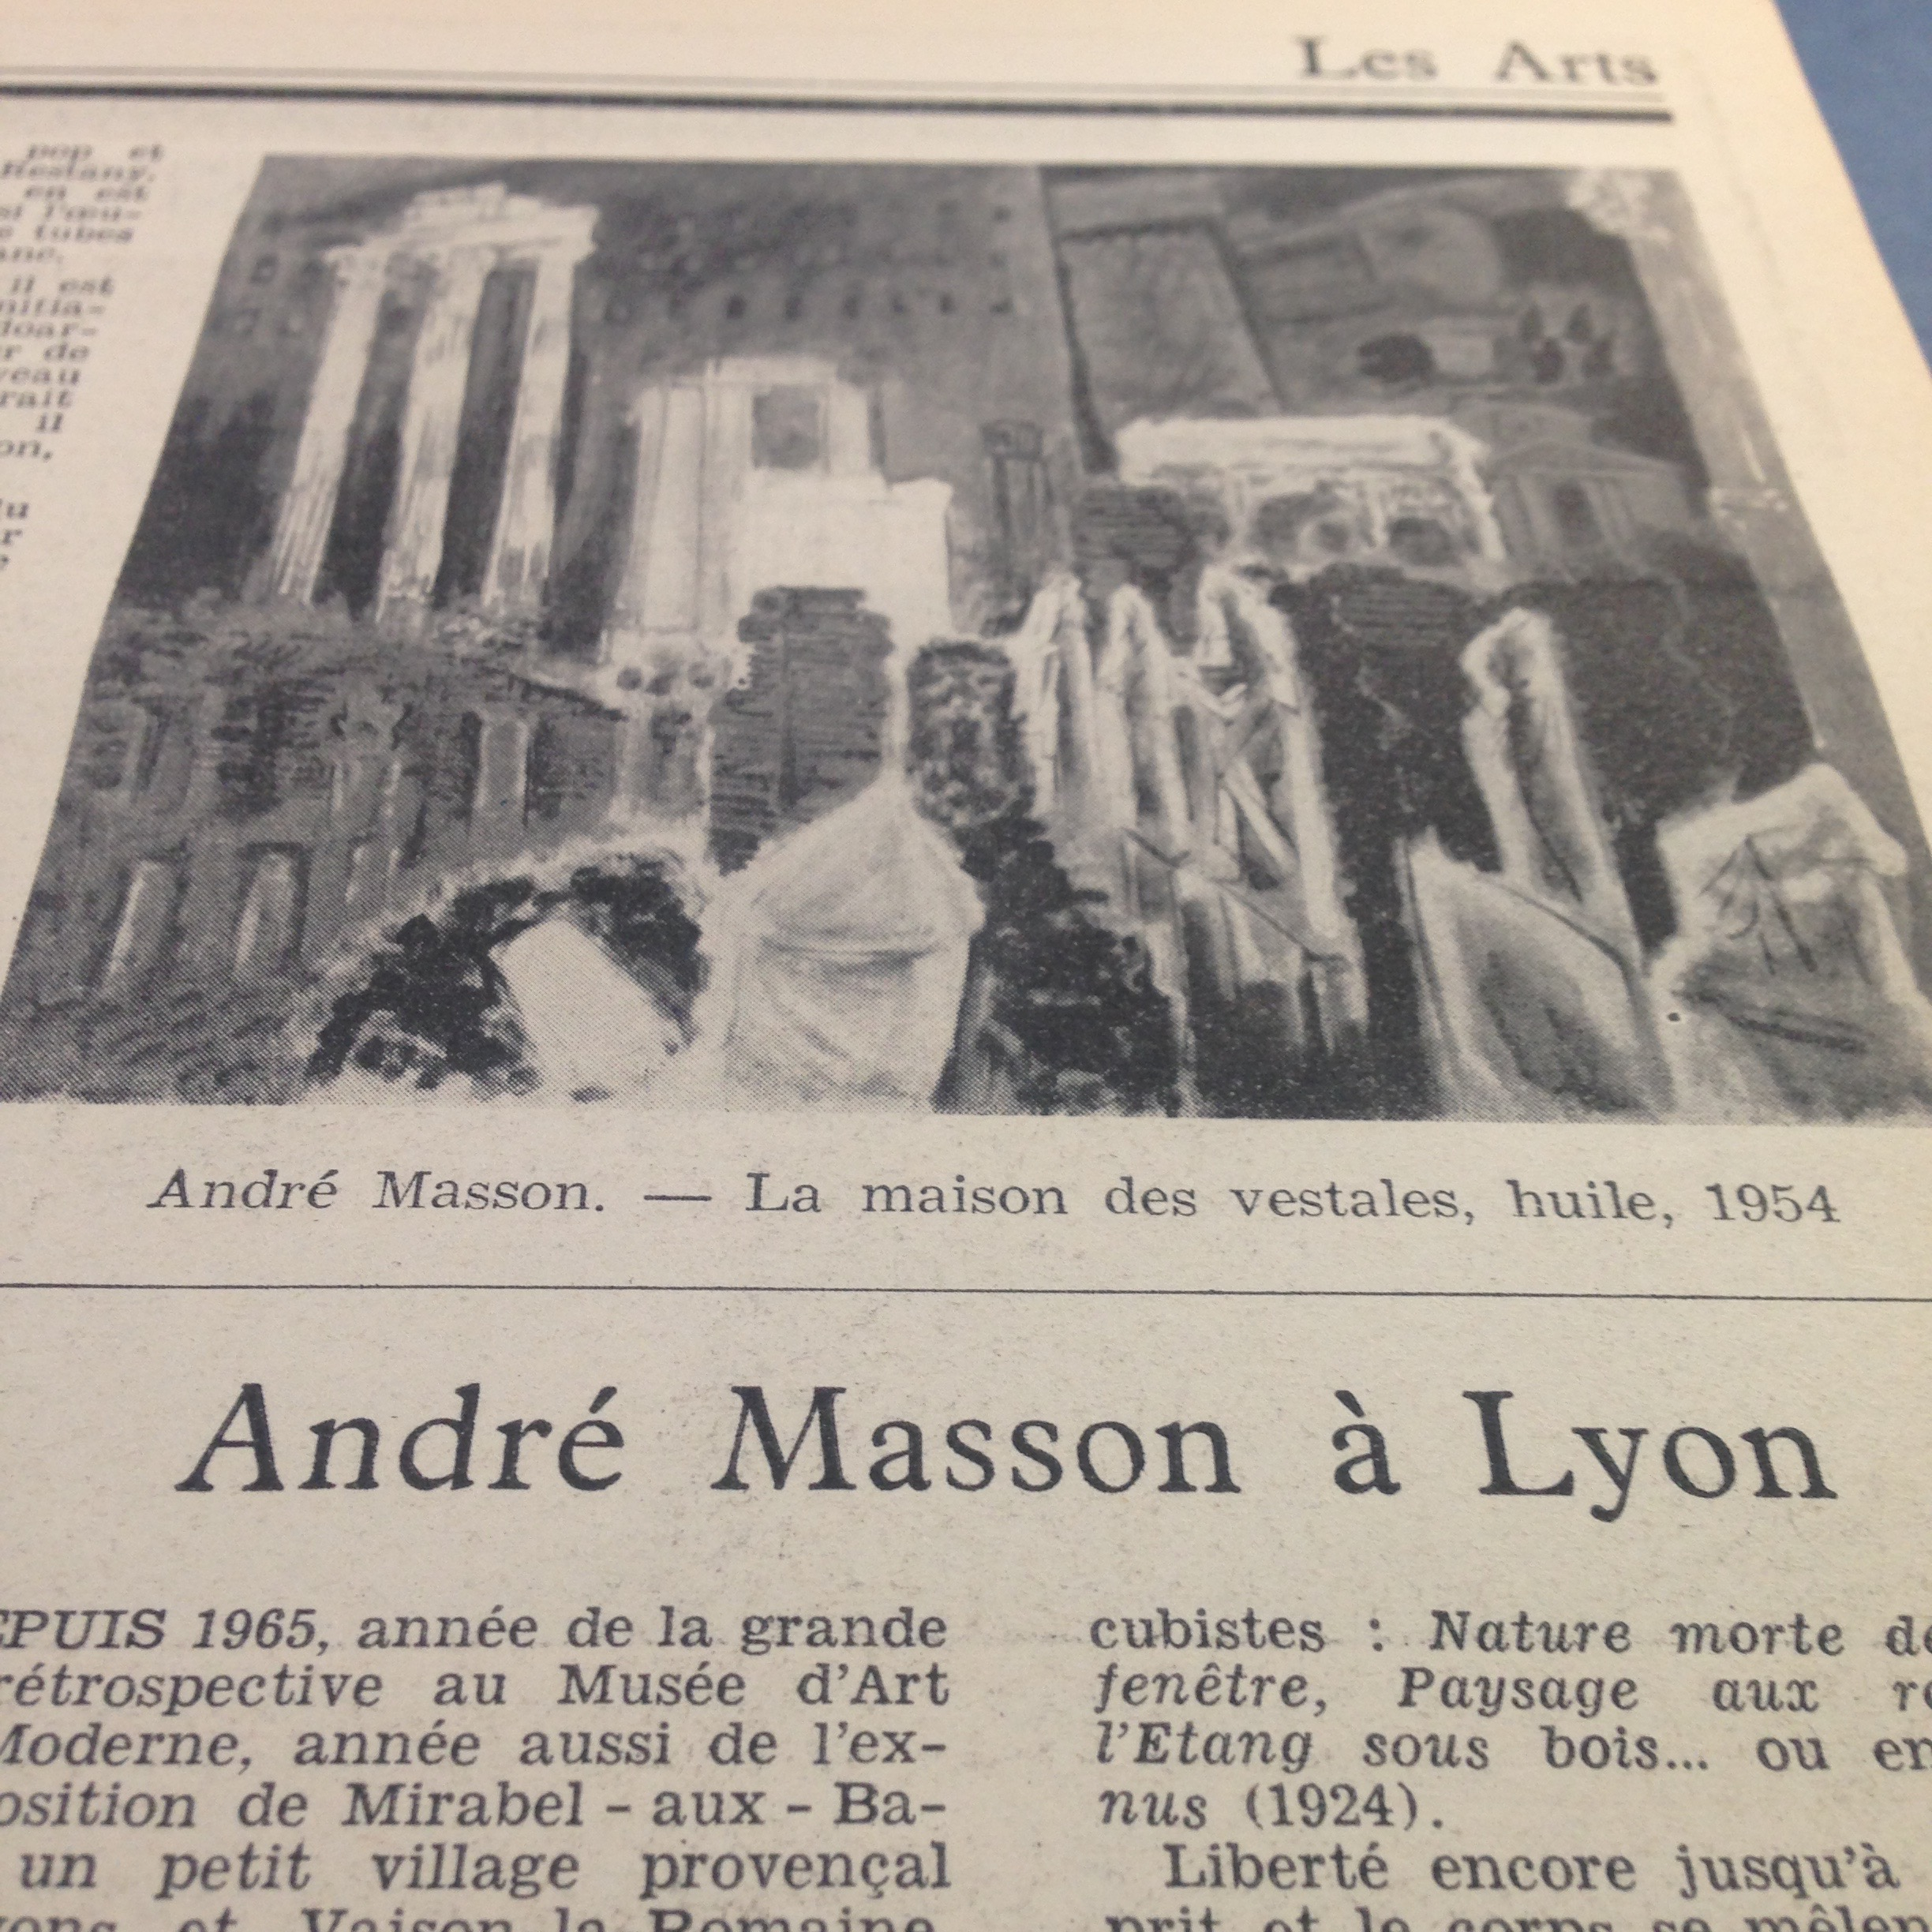
\includegraphics[width=0.33\textwidth]{imagen1190.jpg}
	\caption{\cite{massonlyon}}\label{fig:MassonLyon}
\end{figure}


	Non seulement le sème du mouvement persiste, mais il est l’un des éléments qui insuffle cet état de \enquote{liberté}. De même que \enquote{l’esprit}, dont nous avons vu dans l’organisation du plafond de l’Odéon quelle haute estime et même exigence en a Masson vis-à-vis de son art et de l’homme en général, la faculté de penser est une fois encore juxtaposée au mouvement. C’est presque une expérience synésthésique avec l’oeuvre de Masson, puisque sa faculté de parler à tous les sens ouvre un \enquote{dialogue} avec le spectateur. Cette figure de Masson comme un être libre n’équivaut pas seulement à cette totale expression des sens, mais se lie à une certaine indépendance d’André Masson, atypique en tant qu’artiste malgré son appartenance à des mouvements majeurs. Pour ne pas dire insaisissable, lorsque Guillot associe André Masson et Jacques Prévert : 
\begin{quote}
Mais, même au coeur au surréalisme, André Masson est resté un être “libre“; un peintre “en liberté“. Et je n’ai pu m’empêcher de comparer la position d’André Masson face à la peinture surréaliste à celle de Jacques Prévert face à la littérature ou la poésie surréaliste. Tous deux fidèles à la liberté totale et à l’absence de toutes entraves prônées par le surréalisme, ne “ sortent“ en définitive du surréalisme que parce que, précisément, ils ont su s’en sortir; ils n’en sont issus que parce qu’inconditionnels face à la grande doctrine du mouvement, ils surent s’en échapper!\footcite{massonlyon}\end{quote}
  
Ce rapprochement avec Prévert pour signifier la liberté est d’autant plus symbolique puisque Prévert en apparait comme l’un des plus grands défenseurs, et grand pratiquant du collage, poétique et artistique plus généralement : \enquote{L’oiseau seul et affolé / L’oiseau qui voudrait vivre/ L’oiseau qui voudrait chanter / L’oiseau qui voudrait crier}. Ces vers sont imbriqués dans un assemblage de collages, dépourvu d’oiseau mais avec d’autres signes pour renouer au symbole de la liberté. En particulier le cheval ailé perché sur l’un des monuments d’une photographie de ville d’où émane une lumière comme fond du collage. Une fleur suspendue en l’air, une seconde posée sur l’une des têtes dédoublées du poète en photo et une fée dans les airs en face du cheval. Avec ce dédoublement de signes et de photos du poète, c’est l’assemblage qui le désigne en tant que l’oiseau des vers. Celui qui aspire à la liberté, contre les signes d’oppressions tels que le panneau \enquote{arrêt}. 

	
	 Guillot confirme d’ailleurs ce rapport au corps dans la création chez Masson : \enquote{Liberté encore jusqu’à ce que l’esprit et le corps se mêlent, jusqu’à la réalité et l’imaginaire s’allient}\footcite{massonlyon}. 

	Ainsi, le mouvement des lignes chez Masson est tel que se mêlent l’organique et l’onirique jusqu’à rendre l’un et l’autre indistincts. Cette faculté d’échapper à la catégorisation va jusqu’à rendre selon Guillot les oeuvres de Mason libres totalement, c’est-à-dire ressenties comme telles au seul regard du spectateur : 

	\begin{quote}
	Enfin, il y a ces toiles libres d’elles-mêmes et libres de toute influencer indépendantes et grandes ouvertes sur nos regards. Inclassables comme des expériences  uniques mais indispensables à contempler pour tous ceux qui veulent connaitre tous les méandres, tous les détours, tous les repentirs de cette oeuvre puissante, attentive et courageuse… 	
	\end{quote}
 
	 La personnalisation des oeuvres dans la critique de Guillot induit déjà un dépassement de l’esthétique en tant que tel, en sous-entendant que celle-ci est travaillée en fonction d’une certaine observation des hommes. Et peut-être aussi avec l’attribut « courageuse » d’une image de ce que peut être l’homme, immédiatement perceptible au spectateur.  

En outre, les oeuvres de Masson citées par Guillot pour illustrer cette théorie sont particulièrement représentatives de cette capacité que possède Masson à échapper à la catégorisation : \emph{Tristesse d’une journée de printemps}, conçue en 1956 et composée de sable, tend vers l’abstraction et pourtant son titre préfigure immédiatement le sentiment, structuré selon l’imaginaire du peintre. 

%Mettre illustration "Tristesse d'une journée de printemps": source : André MASSON « TRISTESSE D’UNE JOURNEE DE PRINTEMPS », 1955 - Sable et pigments sur toile, signée en haut à droite, datée et titrée deux fois au dos et sur le châssis - 100 x 81 cm - Provenance : - Galerie Louise Leiris, Paris - Galerie de Seine, Paris - Collection Serge Varène, Paris.

\begin{figure}[H]
   \centering
   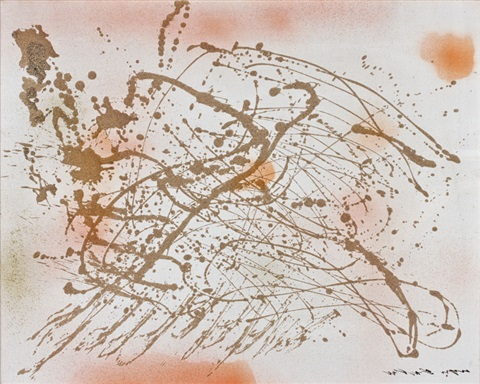
\includegraphics[width=0.33\textwidth]{tristessedunejourneedeprintemps.jpg}
	\caption{\cite{tristesse}}\label{fig:Tristessedunejourneedeprintemps}
\end{figure}

D’autre part, Masson exprime plusieurs fois dans ses \emph{Correspondances} sa réticence pour l’abstrait, qu’il juge trop limité : 

\begin{quote}
Pour moi l’observation de la nature demeure essentielle. Delacroix disait : que la nature était son “ dictionnaire“. Je n’ai jamais pensé autrement. On ne peut rien inventer de toutes pièces et les oeuvres les plus imaginées sont durables dans la mesure où elles restent d’accord avec l’Univers. C’est pour cela que je ne puis accepter, personnellement d’être appelé “abstrait“. Une oeuvre abstraite en peinture serait une oeuvre dans laquelle il n’y aurait aucune allusion à ce qu’on nomme les 4 éléments et les 3 Règnes. Une oeuvre qui ne rappellerait ni les végétaux, ni les animaux, ni l’eau ni le feu, ni la terre ni les cieux ! Mais alors le meilleur tableau abstrait c’est un manuel de géométrie !\footcite[p464]{anneessurrealistes}\end{quote}
 
	La \enquote{liberté }de l’art de Masson particulièrement manifeste pour le chroniqueur Guillot dans cette exposition à Lyon tiendrait donc en partie à échapper à la catégorisation, et ce par le mouvement. \emph{Tristesse d’une journée de printemps} figure le sentiment par le mouvement du sable qui crée la forme, avec des traits tantôt fins tantôt épais à partir des lignes du sable. D’autre part, cet usage du sable ne peut qu’évoquer cette pratique du collage louée par Aragon dès 1939 dans son texte \emph{La peinture au défi}:
\begin{quote}
Tous les peintres qu’on a pu appeler surréalistes, cela aussi est significatif, ont employé le collage au moins passagèrement. […] André Masson a utilisé le sable et la plume, donnant avec celle-ci un effet qui rappelle les anciennes étoffes péruviennes.\footcite[p78]{ecritssurla}\end{quote}	


 	 Il faut dire, ce qui, là-encore, ne tient pas uniquement du propos esthétique, qu’Aragon et André Masson ont tous les deux en commun une certaine réticence vis-à-vis de la toile et la peinture à l’huile. Tout du moins, il s’agit pour l’écrivain et le peintre de ne pas nécessairement privilégier cette technique. 

	Chez Aragon, cette conception rappelle irrémédiablement son passé dadaïste, puisque le groupe tient dans ses Manifestes de 1916 et 1918, ainsi que dans les revues, à abolir la toile, et avec elle l’autorité de l’art. Conception forcément politique, puisqu’elle implique un renversement, une réorganisation des valeurs sociales établies. Mais on peut supposer que cette réévaluation de l’usage de la peinture à l’huile perdure même une quarantaine d’année plus tard, comme un héritage resté du l’expérience, quand Aragon déclare en 1960 : 

\begin{quote}
Il ne me semble pas que la gravité de la démarche picturale tienne à l’emploi de l’huile uniquement. Et personnellement, on le sait, j’ai peu de goût pour l’usage abstrait de ce liquide : on ne s’étonnera pas que j’apporte au moins le même sérieux à examiner la démarche du colleur de journaux découpés faisant des paysages lisibles, que d’autres mettent à discuter du non-dire à l’huile.\footcite{hoffmeister}\end{quote}
 

	 On peut s’arrêter sur la qualification de la peinture à l’huile comme \enquote{abstraite} dans ce texte, c’est-à-dire sans reflets d’une pensée politique. Contrairement aux choix du collage, dès le choix des objets eux-mêmes. Ainsi, même quand le réalisme socialiste n’est plut tout à fait à l’ordre du jour dans l’art d’Aragon, il reste cette dimension réaliste dans ses propres oeuvres comme exigence première, et cette « gravité » de l’art nécessaire pour l’exprimer.

En outre, on peut établir une analogie entre l’écriture de l’article de Guillot pour évoquer les effets de cette \enquote{liberté}dans les oeuvres de l’exposition et les métaphores du tourbillon dans l’article de Boudaille sur le plafond de l’Odéon en novembre 65: 

 \begin{quote}
Ce seront ensuite aux formes que Masson rendra la liberté : elles éclatent, s’engendrent les unes les autres, se déchainent, font voler en minces particules un univers pourtant déjà très tourmenté…Ainsi cette merveilleuse \emph{Constellation érotique} (1961), dans laquelle Masson déploie tout son lyrisme, tout son délire musical et coloré.(\emph{Couple dans la nuit}, 1958, \emph{Constellation des amants}, 1958)	
\end{quote}


	Tant par les titres des oeuvres mentionnées que par le retour chez un autre chroniqueur du mouvement comme tourbillon, Guillot rejoint l’image de Boudaille ouverte dans son article de 65 avec les propres mots de Masson : \enquote{Comme une constellation tourbillonnant}\footcite{avantinauguration}. De cette image omniprésente ressort à la fois une forme de lyrisme cohérente avec le titre des oeuvres autour de la \enquote{constellation}dans le rapport des amants entre eux, romantique ou érotique. 

Ce lyrisme revendiqué s’accompagne aussi de cette force subversive qu’est le tourbillon. D’autant plus que les titres de Masson désignent clairement leur thème autour l’homme, avec une figuration de lignes mouvantes qui laissent deviner sa présence. Sa masse corporelle est détournée au profit de ses lignes de force. Cependant, Guillot n’omet pas de rappeler que cette conception sur la liberté esthétique, et libertaire dans ses nombreuses oeuvres autour de l’érotisme, touche aussi aux faits politiques : 

\begin{quote}
Mais ce baroquisme tumultueux et orgiaque, cette écriture flamboyante et charnelle n’éloignent pas André Masson de notre monde, du monde. En homme libre, il s’inquiète de l’absence de liberté des autres…en Espagne, pendant la dernière guerre. Grande composition sur la \emph{Résistance} (1944) ou admirable ensemble de la \emph{Curée} (1944), Guerre des paysans, vaste évocation de la guerre des paysans allemands pendant la Renaissance (peinte en 1961) ou \emph{Délire lansquenet au calvaire} (1964) se partagent les préoccupations politiques du peintre…\footcite{massonlyon}\end{quote}
 
	L’allusion au baroque, le courant artistique par référence lié au mouvement confirme l’esthétique particulier de Masson en l’associant à l’attribut \enquote{tumultueux}, et cette fois à dessein d’enjeux politiques. Comme l’allusion à la guerre civile d’Espagne, que Masson a vécu, lorsqu’il quitte Tossa del Mar pour Barcelone en Juillet 1936. Ou encore sa toile en hommage l’éloge à la Résistance pendant son exil contraint par sécurité envers sa famille juin aux Etats-Unis. Une forte attirance pour le thème des révolutions se dessine ainsi au cours de ses propres migrations multiples. 

En détournant la représentation directe des hommes et des peuples au profit de leur expression de révolte. Dans \emph{Guerre de paysans}, un arrière-plan rouge vif aux teintes agitées accueille des personnages squelettiques dont la principale caractéristique tant du grand personnage à chapeau, fantomatique, au corps constitué d’une ligne et à la tête carrée que de son voisin grisâtre miniature aux bras écartés dans le bas-droit de la toile, c’est leur bouche grande ouverte. Cette fonction radicalement expressive traversée de lignes blanches et de multiples formes plutôt fantastiques fait surgir un cri de révolte dont la dimension intemporelle des personnages fantastiques dépasse l’époque de la Renaissance. La toile ne dénonce pas tant le cri de révolte manifeste, c’est bien un idéal de cette représentation du peuple auquel aspire le \enquote{baroquisme tumultueux} d’André Masson.

\begin{figure}[H]
   \centering
   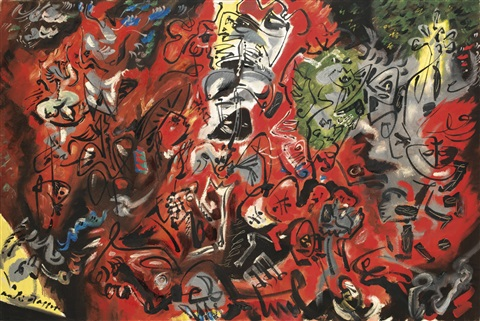
\includegraphics[width=0.33\textwidth]{laguerredespysans.jpg}
	\caption{\cite{massonlyon}}\label{fig:Guerre des paysans}
\end{figure}

%Source image : LA GUERRE DES PAYSANS , 1963- Support : oil-Taille :87,1 x 135,7 cm. (34.3 x 53.4 in)-

	 Ainsi, c’est par une ultime allusion à l’une des grandes oeuvres de Masson que Gérard Guillot conclut sur cette révélation que doit être cette exposition du peintre à Lyon : \enquote{Sur une des routes vers le Sud, l’exposition André Masson doit être une étape solaire : des miroirs en liberté font exploser les limites de notre labyrinthe !} L’image \enquote{des miroirs en liberté}confirme cette vocation presque paradoxale chez Masson de représenter l’homme, plus précisément l’identité en perpétuelle mouvance de l’homme, par une dimension fantastique.

	En outre, la conclusion sur le corps squelettique \emph{Le labyrinthe} de 1938 illustre sur cette référence à Dédale le regard très réfléchi de Masson sur l’homme dans son art, à l’image de son achèvement du plafond de l’Odéon par la figure du penseur comme le souligne Bernard Noël : \enquote{La mythologie qu’élabore André Masson compose une sorte d’encyclopédie plastique de sa pensée}\footcite[p73]{noel}. Et, comme le signifiait symboliquement le regard sur l’homme en train de penser sur le plafond de l’Odéon, avec l’oeuvre du \emph{Labyrinthe}, l’homme est sa propre finalité : 

\begin{quote}
Je trouve “l’âge d’homme“ très important. Tu places l’accent sur l’essence de l’angoisse : la certitude de l’homme d’être enfermé dans sa finitude - Enfermé dans l’arène - labyrinthe, se débattant et s’embrouillant dans sa propre fin.\footcite[p429]{anneessurrealistes}	
\end{quote}
 

\begin{figure}[H]
   \centering
   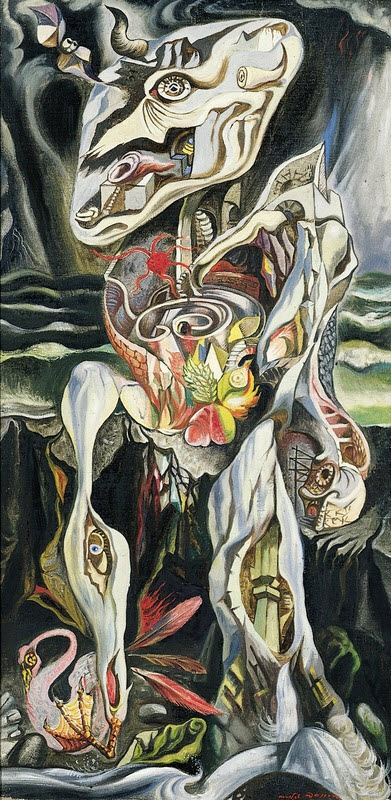
\includegraphics[width=0.33\textwidth]{labyrinthe.jpg}
	\caption{\cite{labyrinthe}}\label{fig:Labyrinthe}
\end{figure}

%Source de la toile : Le Labyrinthe, 1938.- Huile sur toile - 120 x 61 cm - Inscriptions :S.B.DR. : andré Masson- Don Basil et Elisa Goulandris, 1982- Numéro d'inventaire : AM 1982-46 - Centre Pompidou- 

	 Conclure sur une allusion à cette oeuvre de Masson sur l’espace symbolique réservé à l’homme comme un miroir sur lui-même confirme quelle est la finalité des oeuvres de Masson, aussi atypiques les unes des autres soient-elles. On peut ainsi rapprocher ces « miroirs en liberté » des désirs libertaire et de liberté au sens de soulèvement au sein d’une imagerie fantastique qui évoque l’orientation romanesque d’Aragon, notamment depuis 1965 avec \emph{La Mise à mort}. Son miroir du réel bascule lui aussi vers une dimension fantastique avec l’image du miroir. 

André Masson révèle avec cette valeur commune aux deux hommes dans une lettre sur son expérience en Espagne en appelant au lyrisme avec l’imagerie des astres, celle du vertige : 
\begin{quote}
Il y avait un double vertige, l’abîme et le ciel avec les étoiles filantes, le ciel lui-même m’apparaissait comme un abîme, ce que je n’avais jamais ressenti, le vertige du haut en même temps que le vertige du bas. Et je me suis retrouvé dans une espèce de maëlstrom, presque une tempête, et comme hystérique…\footcite{mythologie}\end{quote}
 

	 C’est précisément le mouvement du \enquote{double vertige} qui provoque le basculement vers le fantastique, à l’image du traitement esthétique de Masson sur les désirs personnels et politiques de ses sujets picturaux. Ce n’est donc pas un hasard si dans un articlee d’un autre numéro de 1967 en hommage à Miró, le chroniqueur Hubert Juin rassemble le peintre à André Masson sur un aspect particulier : 
\begin{quote}
Cette liberté devait se payer. Comptant. Il devint beaucoup plus difficile de faire illusion. La peinture était devenue sa propre anecdote. Est-ce à dire qu’elle n’empruntait plus rien au monde extérieur ?  Au contraire. Seule, la servilité était interdite. Son vocabulaire vient de là. Ses racines sont prisonnières de l’épaisseur de la terre, s’y agrippent. Quoi d’autre chez Picasso ? Et chez André Masson, en ceci véritablement exemplaire ? […] Il ne s’agit plus de copier la nature. Il s’agit d’être \emph{comme} la nature. Il s’agit des dire. Il s’agit d’être.\footcite{joanmiro}\end{quote}	 


\begin{figure}[H]
   \centering
   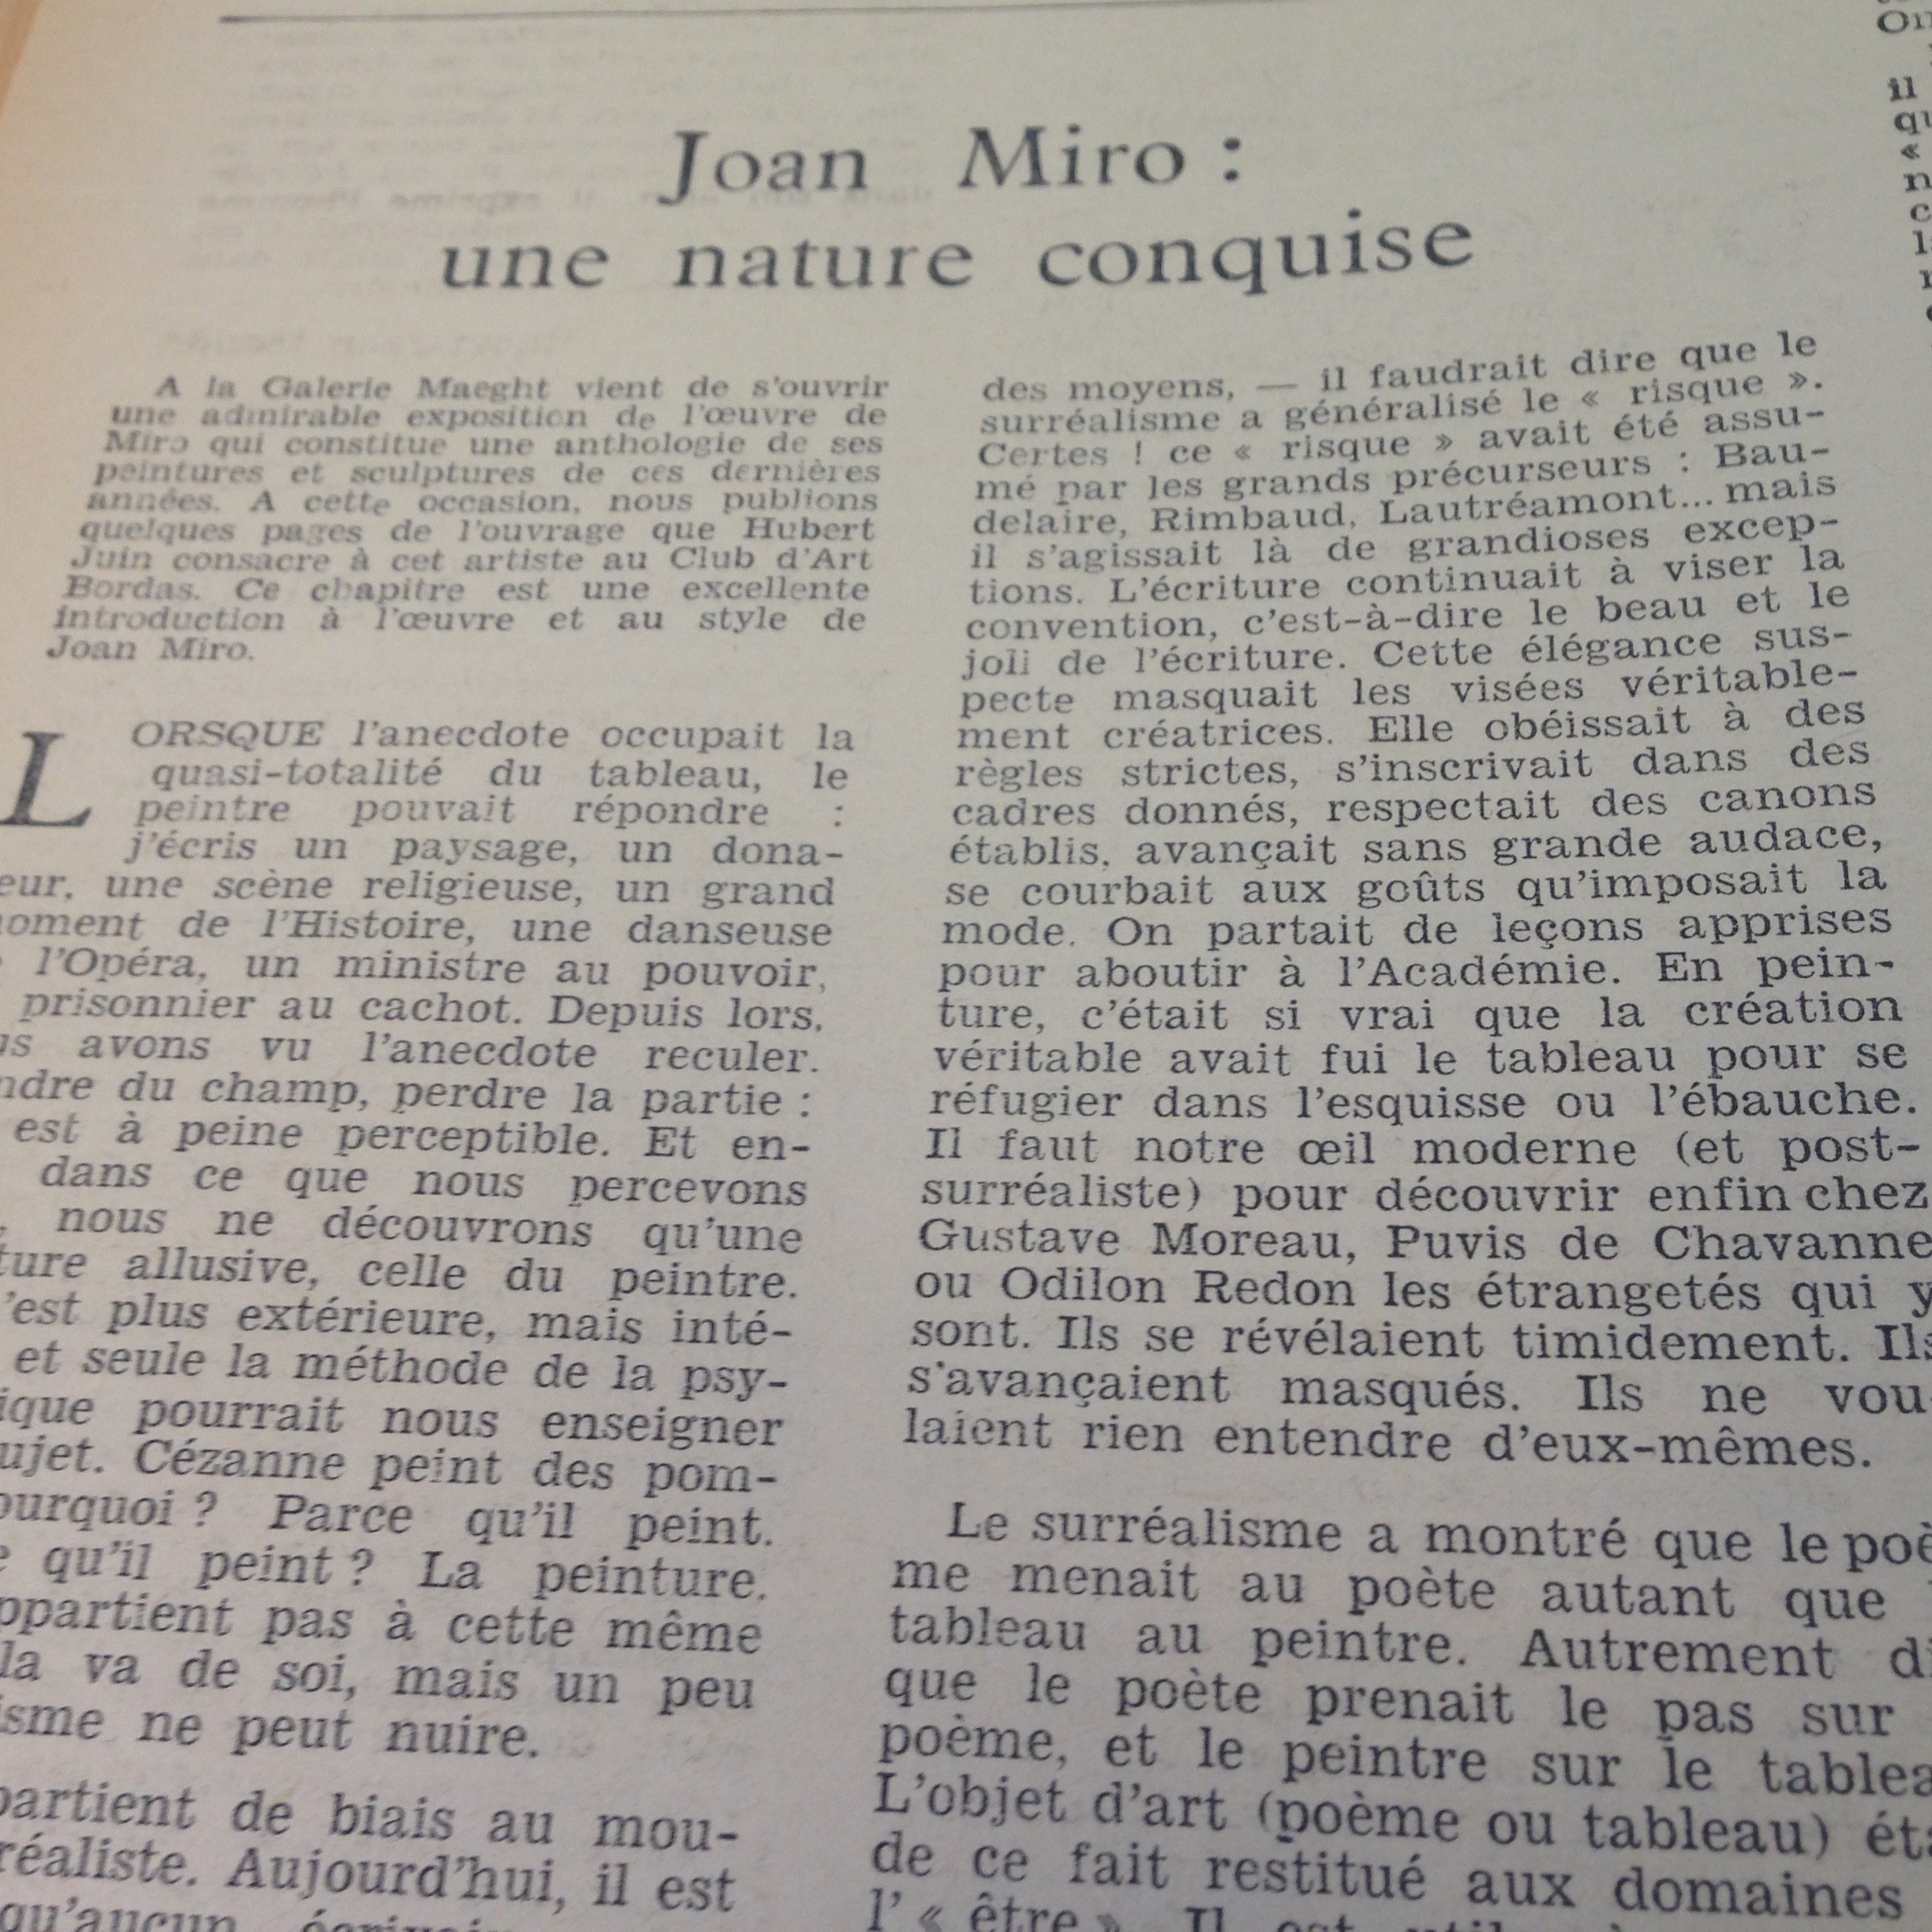
\includegraphics[width=0.33\textwidth]{miron1180.jpg}
	\caption{\cite{joanmiro}}\label{fig:Miro}
\end{figure}

	Ainsi, avec cette recherche esthétique du vertige, André Masson détourne la figuration pour exprimer la nature humaine, et l’on voit selon quelle conception politique cette exigence repose, contre la \enquote{servilité}. 

	L’exploitation de ces puissants sèmes chez différents chroniqueurs des \emph{Lettres françaises} pour traiter le \enquote{baroquisme tumultueux}d’André Masson peut être comparé dans une hiérarchie égale aux journalistes, lorsque André Masson écrit des articles pour le journal. Il intervient deux fois selon deux démarches différentes au cours de l’année 1968. En février, Masson écrit parmi d’autres interventions sur sa vision de Baudelaire, bien que la préface des \emph{Lettres françaises} souligne spécifiquement la qualité de l’écrit de Masson en particulier. 

	Plus tôt, en Janvier, Masson répond à une enquête sur l’art abstrait, basée à partir d’une citation de Malraux. \emph{Les Lettres françaises} n’en sont pas à leur première enquête, ni Masson à sa première participation : Il avait déjà répondu aux côtés d’Elsa Triolet, disposition d’emblée peu anodine sur\emph{Qu’est-ce que l’avant-garde en 1958 ?}. En 1964, \emph{textLes Lettres françaises}publient une immense enquête sur le livre de poche. On peut y retrouver une allusion, comme un clin d’oeil, dans une brève phrase, un paragraphe à elle seule dans \emph{La Mise à mort} un an plus tard : Or, dix ans après l’enquête sur l’avant-garde artistique, l’une des visée de ce questionnement parait clairement de contester la vision de l’auteur sur l’abstrait à partir  de la fameuse citation à commenter par les artistes, André Malraux. 

\subsection{Texte d'André Masson \emph{Baudelaire et les peintres} dans l'article de Georges Besson \emph{Baudelaire et les peintres} (\emph{Les Lettres françaises} [n\degre1220- du 7 au 13 février 1968]) }



Avec ces deux exemples d’écriture dans \emph{Les Lettres françaises} déjà pratiquées par André Masson, il en appelle en 1953 à sauvegarder la figure de Cézanne (entreprise que le chroniqueur Jean Bouret poursuit en 1965, où Cézanne est oublié dans sa propre région) , rend hommage à Turner en 1952. Son intervention dans le journal est le plus souvent pour écrire sur une autre figure artistique. Dans le cas de Février 68, Baudelaire se distingue des autres écrits de Masson dans le journal en ceci qu’il n’est pas peintre. Mais c’est par ses écrits sur l’art que Masson établit un premier rapport entre eux. De fait, la préface de George Besson rappelle que c’est autour de son travail de critique d’art et son analyse de la modernité que la conférence se tenait : \enquote{Du 8 au 13 janvier, s’est tenu, sous le titre :  “Découverte du présent“ un hommage à Baudelaire, critique d’art que nous avons annoncé en son temps.}\footcite{baudelairepeintres}.

% 2 sources *Cézanne : Les Lettres françaises [n\degre473- 9 au 16 juillet 1953], "Cézanne en visite chez Cézanne" après André Masson. (Fait) / *Turner : Les Lettres françaises [n°398- 24 janvier 1952] 


	 André Masson intervient donc une nouvelle fois en tant qu’artiste, mais aussi avec le recul du commentateur d’art. Ses interventions régulières sur le sujet dans \emph{Les Lettres françaises} nous traduisent un certain plaisir de l’artiste à changer de statut pour celui de l’analyste. Et peut-être plus globalement un plaisir de l’écriture, si l’on tient compte de la prolifération d’écrits épistolaires. En outre, le chroniqueur qui présente les différentes interventions, Georges Besson, critique d’art estimé, est aussi l’un des plus anciens chroniqueurs du journal. Depuis 1958, il tient régulièrement une chronique d’art, \emph{Lettre à une Provinciale}. La figure médiatrice de George Besson est donc particulièrement symbolique du lien de Masson avec le journal,comme fidèle des \emph{Lettres françaises} et ami de Masson :
\begin{quote}
Faute de pouvoir reproduire ici les seize communications qui furent lue et les débats qui s’ensuivirent, nous limitons notre publication à des extraits des textes qui nous semblent les plus significatifs, en donnant la plus large place à l’étude d’André Masson qui éclaire la position de Baudelaire, critique d’art, d’un point de vue personnel et original.\footcite{baudelairepeintres}\end{quote}

	En mettant à l’honneur le texte d’André Masson, \emph{Baudelaire et les peintres} George Besson souligne l’intérêt d’une inversion de rôle où le peintre écrit sur le critique, mais pas seulement. Une dimension intime est introduite avant même la découverte du texte de Masson. Et, de fait, l’un des éléments chez Baudelaire qui fascine André Masson s’applique dans le contexte à l’écrit sur l’art, mais il serait possible dans les mots du peindre d’en faire un mode de vie : 
\begin{quote}
Il sait que la sagesse serait de ne rien dire de ce qui ne vous dit rien, la nature et les formes de la sympathie jouant totalement de l’appréciation de l’oeuvre d’art, mais parfois il lui faut passer outre et ne pas craindre les dangers de la partialité volontaire jointe à la “force de la contradiction“.\footcite{baudelairepeintres}\end{quote}

Avec cette idée, on comprend immédiatement le sous-entendu de Besson sur l’aspect \enquote{personnel} et \enquote{original} du texte : André Masson loue une prise de risques de la part de Baudelaire à écrire, y compris quand il n’est pas connaisseur de son sujet. Autrement dit, André Masson préconise cet enthousiasme de l’écrit sur le sujet, au détriment de la dit sagesse. Ne pas craindre l’ignorance. Mais bien plus encore, André Masson fait l’éloge chez Baudelaire d’une écriture subjective, de même qu’il conçoit la réception d’une oeuvre comme étant par essence subjective. Ce \enquote{danger de la partialité volontaire} apparait donc comme étant en réalité une qualité essentielle. Ce qui est déjà un décalage complet vis-à-vis des horizons d’attentes qu’un lecteur aurait envers un critique, et sans doute actuellement encore. 

	D’autant part, non seulement Masson revendique cette subjectivité, tout en ayant conscience de d’autres valeurs autour de la précaution minimalisée, mais les risques mêmes que cette subjectivité apportent deviennent des motifs de réussites dans le travail d’écrit sur l’art. Cette \enquote{force de la contradiction} est clairement revendiquée plus que décriée. D’autant plus avec ce topos commun chez Masson, à dessein poétique et politique dans les notes et critiques de Masson et sur Masson pour décrire ses propres oeuvres. 

	De plus, cette dualité à laquelle aspire André Masson en l’estimant chez Baudelaire prolonge la manifestation des désirs au sens large, comme il la pratique en tant qu’artiste, et comme elle apparait nécessaire selon lui dans la critique. Cette conception est d’autant plus forte si l’on se réfère à la poésie de Baudelaire : \enquote{Il y a dans tout homme à toute heure deux postulations simultanées, l’invocation vers Dieu ou spiritualité et l’invocation vers Satan ou l’animalité.}Autrement dit, cette expression chez Masson une fois encore récompense le désir. 

	C’est d’ailleurs au nom d’une marque d’expression caractéristique chez Masson que celui-ci se projette sur Baudelaire : \enquote{Baudelaire est, profondément, un poète tragique, dénonçant l’ordre factice et l’harmonie conventionnelle. Nul accord parfait, cette âme est pleine de dissonances.}

	Or, cette notion de \enquote{tragique} que Masson attribue à Baudelaire pour qualifier son art est aussi reprise par Paule Gauthier à son propre sujet dans le titre d’un autre article dans un numéro ultérieur en mai 68, \emph{La sérénité de l’expression tragique d’André Masson}\footcite{expressiontragique}.De plus, au nom de la dimension \enquote{tragique} de sa poésie, et toujours contrairement à un horizon d’attente sur toute oeuvre,l’harmonie n’est pas un idéal. Tout au contraire, dans ce topos musical, elle est mise à mal par la rupture, le désordre. A l’opposé d’une symbiose parfaite, fausse, et surtout sans réflexions.


	
 Le tragique de Baudelaire comme pour Masson impliquerait donc par essence une révolte, c’est-à-dire l’idée de briser cette convention de l’ordre que dénonce Masson. Une nature politique est ainsi attribuée à l’imitation d’une action noble qu’implique initialement sa définition dans \emph{le Traité de la Poétique} d’Aristote. Or, l’action noble n’est plus le maintien de l’ordre, mais son bouleversement. Par conséquent, parler de Baudelaire dans ce texte évoque la position du spectateur devant un tableau de Masson : 

\begin{quote}
 Les puissances de l’imagination et par conséquent la force de l’image, son irruption dans notre coeur et dans notre esprit font partie pour Baudelaire du poète sacré. Pourtant, il n’est d’image que de l’homme. Le peintre-poète obéissant à son intuition lyrique projette dans la nature ses pulsions les plus vives afin qu’elle atteigne à son identification. Les ciels tumultueux, les coups de théâtre de la foudre, la fureur des \enquote{décors} ou \enquote{toiles de fond} mais accompagnements emblématiques de la Passion humaine.\footcite{baudelairepeintres}\end{quote}
 
 Il est intéressant de voir comment Masson détourne la valeur d’abord spirituelle du \enquote{poète sacré}pour au contraire revenir à échelle humaine avec cette vérité générale, et surement le fondement de son art : Tout ramène à l’homme. 

	L’homme pour Masson, c’est aussi ce à quoi l’homme aspire, cette \enquote{Passion humaine}. Cette finalité, tant artistique que philosophique, est aussi l’homme en tant que tel. On voit dans le déchainement dans la propre envolée lyrique de l’écriture de Masson, par successions de métaphores, comment la figure de Baudelaire a éveillé sa propre Passion : Ce topos du théâtre n’est pas seulement un imaginaire intime, il est aussi une référence aux projets de Masson avec Jean-Louis Barrault sur les décors et les costumes de pièces, le plafond de l’Odéon, sans compter ses allusions précédentes à la tragédie. Le théâtre va donc de pair avec avec un autre fameux topos proprement au mouvement Romantique pour signifier la Passion autour de la foudre, les métaphores autour du déchainement météorologique. Les chroniqueurs des \emph{Lettres françaises} évoquent donc l’oeuvre de Masson avec le même discours qui est celui de Masson lui-même pour signifier la Passion humaine. 

Avec ce parti pris des choses exigé dans les oeuvres d’art et tout sujets, André Masson rattache cette valeur à une certaine tradition philosophique. Kant, dans sa \emph{Critique de la raison pratique}, conçoit la passion comme une entité réflexive, \enquote{La passion se donne le temps et, aussi puissante qu’elle soit, elle réfléchit pour atteindre son but.}. Concept que rejoint André Masson en associant l’acte de la pensée à la pulsion du traitement de ses sujets. Dans son \emph{traité de la nature humaine}, Hume associe également la passion aux émotions, mais aussi aux idées et à la réflexion : \enquote{Les questions de l'entendement et des passions font à elles seules une suite complète de raisonnements, et j'ai eu envie de tirer parti de cette division naturelle pour tester le goût du public.}\footcite{hume} Ainsi, rien d’anodin chez Masson à reprendre cette notion philosophique au regard de ces penseurs du XVIIIème siècle, avec dans sa propre exigence de peintre et de critique l’entremêlement de la force de l’oeuvre et son lyrisme. 



	Avec une telle philosophie, il apparait clairement que la doctrine d’André Masson est idéologique, et non dans celle du matérialisme communiste. André Masson conclut d’ailleurs sur cette anecdote qui révèle dans son passé surréaliste cette perpétuelle volonté de jouer de références pour construire la réflexion du mouvement : \enquote{Je disais un jour à Paul Eluard : “Le père de notre Eglise ce n’est pas Rimbaud, c’est Baudelaire“. J’ajoute qu’il m’approuva sans réserve}.Distinction ici avec Aragon, dont Rimbaud est avec Lautréamont l’une des grandes références dès ses premières rencontres avec Breton. La passion qu ‘à Masson d’user de références de figures fortes pour incarner le surréalisme s’appuie sur des moments dans l’Histoire qui répondent manifestement à ses propres idéologies. Paradoxalement c’est pour les mêmes raisons qu’Aragon s’attache à la figure de Rimbaud que Masson lui préfère Baudelaire. Un rapport intime pour une figure qui incarnerait la passion, en particulier celle de la révolte. 

	Mais la réelle distinction entre Rimbaud et Baudelaire chez Masson se fait probablement avec l’idée du \enquote{tragique} : Françoise Lavaillaint rappelle la nature profondément angoissée d’André Masson, répercutée dans son art et ses relations intimes. En particulier amoureuses, lors de mouvements brusques et parfois violents de son humeur. Bernard Noël montre comment cette angoisse produit le vertige : \enquote{Ce délire aiguillonne le travail Masson et le conduit à l’excès, à la violence, au tragique, non pour les cultiver, mais pour obéir à un emportement profond et naturel}\footcite[p83]{noel}.  Ainsi, de même que ses oeuvres sur l’essence de l’homme, Masson révèle dans son texte sur Baudelaire un nature profondément idéologique qui révèle ses propres traits esthétiques. De même qu’à l’inverse dans son art pictural, l’esthétique mouvementée conduit à son impulsion idéologique. 

C’est un constat analogue que l’on peut tirer dans la brève mais efficace réponse de Masson à l’enquête sur l’art abstrait quelques mois plus tôt en Janvier 1968. On peut se demander si cette enquête sur l’art abstrait n’est pas un clin d’oeil à l’enquête sur les avant-gardes (\emph{Qu’est-ce que l’avant-garde en 1958 ?}\footcite{avantgarde}), dix ans auparavant.La réponse d’André Masson à l’époque, un bloc de texte qui occupait la première page du numéro conjointement avec celle d’Elsa Triolet, était déjà claire et non sans ironie sur le terme débattu : \enquote{L’AVANT-GARDE ? Mais elle n’existe pas sans une arrière-garde.} L’enquête de 68 est présentée de façon très écolière par la préface, avec une citation et une réponse dialectique : 

\begin{quote}
Dans une récente interview à l’un de nos confrères, André Malraux a dit : “L’abstraction a a représenté la plus grande liberté possible pour le peintre. Mais c’est une école. Elle cessera comme toutes les écoles“. Voulez-vous répondre aux questions suivantes :  I) - Considérez-vous que l’abstraction soit- ou soit devenue- une école ? Qulle que soit votre réponse, dans quel sens comprenez-vous le mot “école“ ?  II. - Quel a  été dans le passé, quel est aujourd’hui l’apport de l’abstraction à l’art du XXème siècle ? III.-Comment envisagez-vous sa fin ou ses développements éventuels ? Et existe-t-il ,à vos yeux, une forme d’art susceptible de succéder à l’abstraction ou de la remplacer ?\footcite{avantgarde}
\end{quote}
 
	 La réponse concise de Masson, en mauvais élève, tient cette fois en une phrase, aussi synthétique qu’énigmatique, comme le suggèrent les points de suspension : \enquote{Masson dit “On peint pour \enquote{être} même fugacement. C’est de cette leçon que l’école du Pacifique est née…“}. Quand on se remémore plusieurs lettres moqueuses de Masson sur l’art abstrait, comparant régulièrement cette esthétique à un « manuel de géométrie », Masson, grâce à cette allusion, réfute l’art abstrait par l’affirmation. Il le fait en énonçant sa propre conception de la finalité de l’oeuvre (\enquote{on peint pour}). Il en demeure qu'André Masson et ses esquisses opèrent un fil médiateur entre les deux intellectuels. Ses esquisses ne sont pas moins que la trace d'une conviction esthétique profonde commune à Aragon et Malraux dont elles sont le symbole. On retrouve d'ailleurs dans les mots de Malraux sur l'esquisse quelques orientations idéologiques qui ne sont pas sans rappeler le combat de toute une vie de Masson si l'on pouvait lui en attribuer un : 

	 \begin{quote}
	 Non que l’esquisse fût tenue, par avance, pour supérieure à l’oeuvre terminée. Il s’agissait d’esquisses d’une nature particulière, parentes de l’Adoration des mages de Léonard, de certains Rembrandt “inachevés“, de presque tous les Daumiers. On peut douter que les esquisses des portraits de Raphaël aient été de cette nature; l’esquisse d’Ingres pour sa Stratonice est inférieure au tableau de Chantilly; mais ces dernières esquisses, qui sont des préparations, des états du tableau, sont soumises à ses lois. Alors que les esquisses de Rubens ne sont pas seulement des états; alors que celle de la Bataille  de Taillebourg est soumise aux lois de Delacroix, et le tableau achevé, aux lois de la critique et à un accord avec le témoignage de nos sens, au traditionnel illusionnisme que Delacroix, dans son Journal, n’ose pas récuser tout à fait. […] L’art entre en conflit avec le “fini“, avec le témoignage de nos sens, avec la peinture en tant que représentation des spectacles.\footcite[p56]{museeimaginaire}\end{quote}

	Ce rapport de force entre l'esquisse et la toile est décrite par Malraux avec le topos de la soumission. Cette notion, que l'on imagine avant tout politique, incarne d'une manière générale le constant refus d'André Masson de céder à cette même soumission. Tout son art, sans compter sa sensibilité politique, est dirigé contre lui. Comme le manifeste ses notes dans sa \emph{Mémoire du Monde} sur ses fugues sur le champ de bataille, et les tentatives d'échapper aux hopitaux psychiatriques. Sans oublier certains doutes sur les thèses marxistes précédemment évoquées.
	
	\subsection{André Masson : Passerelle entre Aragon et André Malraux }
	 Le parti pris de l'esquisse chez Masson, le goût prononcé de l'inachevé, pourrait s'expliquer en partie par l'idée de prendre position dans cette dualité énoncée par Malraux pour l'inachevé, qui comporte chez Masson probablement une part d'inssaisissable, une prise de liberté du trait par l'esquisse. Et, de même que l'obsession du thème de la métamorphose est un signe récurrant chez Masson, liées à leurs précédentes collaborations autout de l'érotisme, de même le thème de la métamorphse lie intimement les créations de Masson et un projet tel que celui du \emph{Musée imaginaire} :\enquote{Le Musée imaginaire naît d’une métamorphose aussi profonde que celle dont naquirent les premières collections italiennes : comme les dieux antiques lors de la Renaissance, les dieux qui ressuscitent devant nous sont amputés de leur divinité}\footcite[p179]{museeimaginaire}. Une telle définition peut se confondre dans le projet visuel de Masson qui fait de la métamorphose une autre réalité, le revers du visible.  Cette spéficité propre à Masson de la métamorphose et la sensiblité à l'esquisse le désigne comme figure médiatrice entre Aragon et Malraux. 
	

	L'exemple de la collaboration entre Aragon et André Masson Pablo Neruda en décembre 1965 a l'avantage d'éclairer sur ces rapprochements connus mais moins marqués dans les mémoires que ceux de la période surréaliste qui a pourtant tout autant dans une autre mesure marquée les esprits de personnalités autant impliquées dans le conflit de la guerre civile d'Espagne que ne l'auront été André Masson, Aragon, et André Malraux. L'engagement de Masson et Aragon particulièrement manifeste un rapprochement idéologique quelques années après les distinctions de prises de positions vis-à-vis du parti communsite, et possiblement un deuxième temps d'amitié entre les deux hommes auquel ce numéro de décembre 1965 rend aussi hommage. 
	

Mais peit-être faudrait-il comparer, face à cette proximité esthétique chez Aragon et chez Masson pour l'esquisse, ce parti pris des \emph{Lettres françaises} réservé tout particulièrement pour André Masson, comparer les propos d'Aragon et de Malraux sur le sujet la même année en 1947. D'une part, avec Aragon, dans sa préface aux\emph{Dessins de Fougeron}, et dont l'on soupçonne que de 1947 jusqu'en cette période de décembre 1965 si cette ligne politique et esthétique du trait varie mais n'en demeure pas moins obsédante et essentielle à ses yeux. Avec Malreux d'autre part, qui écrit la même année \emph{Les voix du silence}, dont l'oeuvre inscrite dans le projet du \emph{Musée imaginaire} est rééditée cette même année de 1965. Le développement qu'y consacre Malraux au sujet de l'esquisse n'est pas sans rappeler et même rejoindre quelques convictions esthétiques et idéologiques d'André Masson. Les deux hommes sont d'ailleurs amis et ont collaboré ensemble sur une oeuvre telle que \emph{Les conquérants} en 1949. André Masson agirait ainsi comme une figure médiatrice entre ces deux intellectuels, mais dont l'on retrouve dans les lignes de Malraux une vision commune sur l'esquisse et ce qu'elle implique, à commencer en matière d'esthétique : 

\begin{quote}
 L’esquisse est, en principe, un “état“ de l’oeuvre antérieur à son achèvement, à l’exécution de ses détails surtout. Mais il en existe un type particulier : cela où le peintre, ne tenant pas compte du spectateur et indifférent à l’illusion, a réduit un spectacle réel ou imaginaire à ce par quoi il devient peinture : taches, couleurs, mouvements.\footcite[p52]{museeimaginaire}\end{quote} 

Malraux conçoit ainsi l'art de l'esquisse comme l'étape du détail par excellence, ce qui peut paraitre au premier abord paradoxal avec sa nature inachvée qu'il lui reconnaît tout autant. Tout comme Aragon dans sa préface aux \emph{Dessins de Fougeron}, l'esquisse n'est plus une étape ni même un enjeu vis-à-vis de la peinture, elle est son processus :

\begin{quote}
Et l’on vit le maître épouvanté de sa maîtrise imiter à grand peine la maladresse de l’élève, le tremblant devenant le témoin de l’émotion sacrée, l’accident l’essentiel, l’inachevé seule satisfaction. […]C’est peut-être pourquoi je me méfie des peintres dont on ne voit jamais les dessins. Que me cachent-ils ? Pourquoi ne veulent-ils pas que je voie le squelette de leur pensée ?\footcite[p133]{ecritssurla}\end{quote} 

Il est intéressant que ce que Malraux décrit comme un \enquote{état} marquée par le détail, pour ne pas dire le moment où l'artiste révèle sa spécificité, Aragon en vient à la même conclusion avec un registre plus lyrique, expliqué en partie du fait que la marque de l'artiste ne vient pas de sa rigueur mais de, \enquote{la maladresse}, \enquote{l'émotion sacrée}, \enquote{l'accident} dont ces aspects semblent se résumer dans la notion d'\enquote{inachevé}. Masson incarne ainsi avec sa recherche de \enquote{l'illimité} la frontière entre le vertige argonien et la métamotphose du musée imaginaire, ce double projet entre Masson et Malraux de métamorphse de l'oeuvre mais aussi la \enquote{métamorpose du regard} : 

\begin{quote}
« Il va de soi que l’immense métamorphose qui avait fait, de la volonté d’exprimer le surnaturel, une maladroite intention d’imiter la nature - instituant celle-ci juge du surnaturel, et effaçant ainsi un millénaire d’art chrétien - était inséparable d’une métamorphose du regard. La création de tout grand art est inséparable d’une telle métamorphose, qui n’appartient point au domaine de la vision, mais de l’attentionnée et d’une sorte de projection sur l’oeuvre, qui mène le spectateur à y reconnaître ce qu’il en attend, fétiche ou statue.\footcite{p201}\end{quote}

L'appréhension d'un nouveau regard sur l'oeuvre est intimement liée à l'utopie chère à Masson et Malraux de quitter la référence de la nature, pour tendre chez Malraux vers le sacré, ce qui n'est pas si éloigné de l'expression \enquote{fête pour les yeux } chère à Masson empruntée dans le journal de Delacroix. 

	 Et peut-être Pablo Neruda est-il une autre de ces présences médiatrices entre Aragon et Masson, pour cette sensibilité et ce combat commun pendant la guerre d'Espagne, l'événement symboliquement enfoui derrière celui du tremblement de terre du Chili qui fait perdre à Neruda sa maison auquel leur collaboration est dédiée. 

	Cette question de l'esquisse en 1965 où Masson figurerait la passerelle entre Aragon et Malraux illsutre aussi l'évolution de la perspective politique abordée dans \emph{Les Lettres françaises} dans les années 1960, toujours aussi ancrée dans ce journal culturel, mais reconsidérée sans le réalisme socialiste qui influençait son discours dans son texte dédié aux \emph{Dessins de Fougeron}. Cette évolution est relatée par Philippe Olivera dans son article centre sur les années de 1958 à 1968 du journal : 


	\begin{quote}
		
	\end{quote}

% ajouter la référence de l'article d'Olivera (pdf) 

Ainsi, le geste du dessin qui jouait un rôle fondateur dans le texte d'Aragon sur les dessins de Fougeron évolue même après le déclin du réalisme sociliste. Et peut-être son rapprochement idélogique notamment au sein du journal avec André Masson comme le symbolise leur collaboration autour de la figure de Neruda illustre aussi l'évolution de sa formule, \enquote{ Oui, c’est le destin de l’art figuratif qui se joue à chaque dessin.}\footcite[p135]{ecritssurla} Toujours est-il que cette conviction de favoriser le dessin à la toile, l'inachevé à l'achevé, reste une profonde conviction communiste chez Aragon mais qui remonte déjà au moins jusqu'à la période de la jeunesse surréaliste chez Masson comme chez Aragon, pour finir par être l'un des motifs de rassemblement entre les deux hommes dans ces années 1960 parmi les jeux d'échos de leurs correspondances opérées par \emph{Les Lettres françaises}

	Or, c’est justement l’absence de finalité qui provoque dans ses correspondances le scepticisme de Masson pour l’abstrait, avec ce topos  de la géométrie. L’adverbe \enquote{fugacement} pourrait toutefois évoquer le mouvement vif du trait qui jaillit propre à l’esthétique abstraite. Si ce n’est qu’elle est surtout caractéristique sous la plume de Masson comme d’un mode de figuration pour incarner l’homme. 

	La référence avec l’Ecole du Pacifique au Nouveau Réalisme, né seulement quelques années auparavant, est un mouvement qui revendique d’exister par sa singularité. L’allusion au Nouveau Réalisme comporte à la fois l’héritage de Dada, dans un journal qui cite Tristan Tzara régulièrement et le mouvement régulièrement, et la vocation d’une nouvelle composition du réel explique amplement l’empathie de Masson pour ce mouvement en pleine expansion. C’est donc à plusieurs échelles que Masson intervient et que son oeuvre se manifeste l’année 1968. Il est intéressant de constater qu’il occupe une place de plus grande ampleur encore que les années précédentes en cette année aussi riche d’événements politiques. Comme \emph{Les Lettres françaises} vont convoquer naturellement Courbet pour parler de la Commune, l’oeuvre d’André Masson et ses interventions occupent régulièrement les numéros dans ces mois de tension politique. 

	Enfin, avec ce jeu de chassé-croisé des écrits respectifs d’André Masson et d’Aragon dans \emph{Les Lettres françaises}, leur collaboration affichée confirme quelle visée esthético-idéologique poursuivent les deux hommes avec des processus distincts.

\section{La collaboration d’Aragon et Masson dans le journal, réactualisation sentimentale et politique d’engagements historiques communs}

Cette collaboration entre André Masson et Aragon en décembre 65 est hautement symbolique autant par la forme que par le sujet : Aragon intervient non en tant que critique mais poète, Masson comme dessinateur, avec l’une de ses esquisses comme aiment à les utiliser \emph{pLes Lettres françaises}. Et, plus précisément, la légende de l’esquisse de Masson présente ces vers d’Aragon de\enquote{première étude}.\footcite{pabloneruda}

	 Le propos ensuite autour de la figure de Pablo Neruda incarne un événement politique et historique notable mais vécu intimement par les deux hommes. Tous deux ont pris part à la guerre civile de 1936 du côté des républicains. André Masson vivait avec sa famille en Espagne. Aragon rencontre Pablo Neruda pendant la guerre civile en 1937. Ces aspects montrent bien quelle dimension personnelle avait pris cette bataille politique de défense idéologique. Or, au coeur de ce combat politique, c’est par la voie intellectuelle et politique que la rencontre se produit, d’après l’article de Laetitia Boussard sur la relation entre Aragon et Pablo Neruda :


\begin{quote}
Leur rencontre a lieu en France, à Paris, en 1937, dans le contexte de la guerre civile espagnole. Ils font partie du groupe d’intellectuels, lisons-nous dans Confieso que he vivido, qui prépare un congrès devant se dérouler à Madrid et qui réunirait des écrivains anti-fascistes du monde entier. Louis Aragon offre d’ailleurs à Neruda un emploi dans son association, l’aidant ainsi à subvenir à ses besoins. Tous deux s’engagent dans la lutte antifranquiste, Louis Aragon en convoyant des dons de l’association internationale des écrivains pour la défense de la culture, Pablo Neruda en préparant le départ de républicains espagnols pour le Chili à bord du Winnipeg en 1939. Ils se rencontrent dans un contexte historique particulier qui les réunit dans leur lutte contre le fascisme et qui donne naissance chez le poète chilien à España en el corazón, recueil de poèmes publié en 1937 au Chili, puis en France en 1938, préfacé par Louis Aragon. España en el corazón deviendra en 1948 le titre d’un poème dans le \emph{Nouveau Crève-Cœur}.\footcite{aragonaneruda}\end{quote}	 

L’histoire même de leur rencontre, et les prolongements de contact tant \enquote{transtextuels} que sociaux qui ont perduré, implique Pablo Neruda dans cette affirmation chère à Aragon de fixer son identité politique à partir de sa pensée poétique. Leur rencontre est le symbole de cette conception aragonienne. En outre, la légende du dessin d’André Masson rappelle un autre événement arrivé à Pablo Neruda en 1965, le \enquote{tremblement déterre du Chili au début de cette année où la maison du poète a été détruite}\footcite{pabloneruda}. En somme, Pablo Neruda est présenté par cet événement comme un poète nomade. Il est intéressant que le tremblement de terre et ses conséquences ait inspiré la création d’Aragon comme d’André Masson. Ce dernier, comme nous l’avons vu dans d’autres esquisses, mais aussi dans les métaphores astrales de ses écrits, est particulièrement attiré par le processus d’explosion et de jaillissement, autant dans le processus de création que dans la réception de l’oeuvre qui mit se vivre comme une révélation. L’oeuvre poétique de Pablo Neruda aspire à la même forme d’expressivité que les dessins d’André Masson, celle du ressenti de l’homme sur le monde :

\begin{quote}
Le poète au contraire, met par nature au pluriel, il salue avec amour l’infinie multiplicité de l’Etre, il vitrer il nourrit sa pensée et son chant, d’un échange généreux et perpétuel : “Je est un autre“, dit-il sans cesse avec Rimbaud. Aussi “le culte des images“ est-il chez lui non une fuite devant le monde, mais l’affirmation la plus haute du lien qui unit l’homme et le monde, et comme l’annonce faite à l’homme de son pouvoir possible sur le monde.\footcite{marcenac2004pablo}\end{quote}	


	Les deux hommes partagent la conviction puissante au fondement de leur oeuvre d’un réel qui ne peut pas être la reproduction de la Nature. Cette orientation est liée à une idée commune chez Neruda, Masson, et Aragon particulièrement en cette année 1965 riche d’allusion dans \emph{Les Lettres françaises} à \emph{La Mise à mort}, d’une identité altérée, multiple, et en partie irrationnelle. Comme pour l’oeuvre de Masson, celle de Neruda comporte dans cette idée de l’homme une dimension de transformation du monde. Ainsi, l’élan et le mouvement sont au coeur de leur imaginaire. Or, c’est peut-être parce que les recherches d’Aragon et André Masson n’ont jamais été aussi proches dans leurs oeuvres respectives qu’en 1965 que tous deux collaborent pour cet hommage à Pablo Neruda, et pas seulement pour un riche passé politique commun pendant la guerre civile d’Espagne en 36.  Toujours est-il que le dessin d’André Masson, s’il fait référence à l’événement précis du tremblement de terre, cherche à faire image exactement de la même façon qu’Aragon et son poème \emph{Le Paresseux} reproduit dans cet article. C’est d’ailleurs suite à l’événement de la perte de la maison de Neruda suite au tremblement de terre dans le Chili qu’Aragon publie le recueil \emph{Elégie à Pablo Neruda} dont est extrait ce poème. 


Croiser la réception d’Aragon avec \emph{Le Paresseux} et l’esquisse d’André Masson montre la perception romantique des deux hommes sur cette catastrophe naturelle. Romantique, parce que c’est une image spécifique du poète qui en résulte : « Continueront voyager choses / de métal entre les étoiles ». Ainsi commence Le Paresseux, et cette image lyrique des morceaux de métal au milieu des astres substitue à la tragédie météorologique une dimension poétique. Cette fameuse métaphore astrale si chère à André Masson dans ses écrits, notamment pour évoquer ses oeuvres, est traduite dans son dessin minimaliste, fait de petits bonhommes et de traits vifs, par la figuration d’une étoile sur la partie centrale du haut du dessin, au sommet du croisement des lignes. Comme souvent dans les dessins de Masson, celui-ci paraît rechercher la simplicité maximale, tout en demeurant une énigme. Tout au moins, pas immédiatement compréhensible au premier regard. 

\begin{figure}[H]
   \centering
   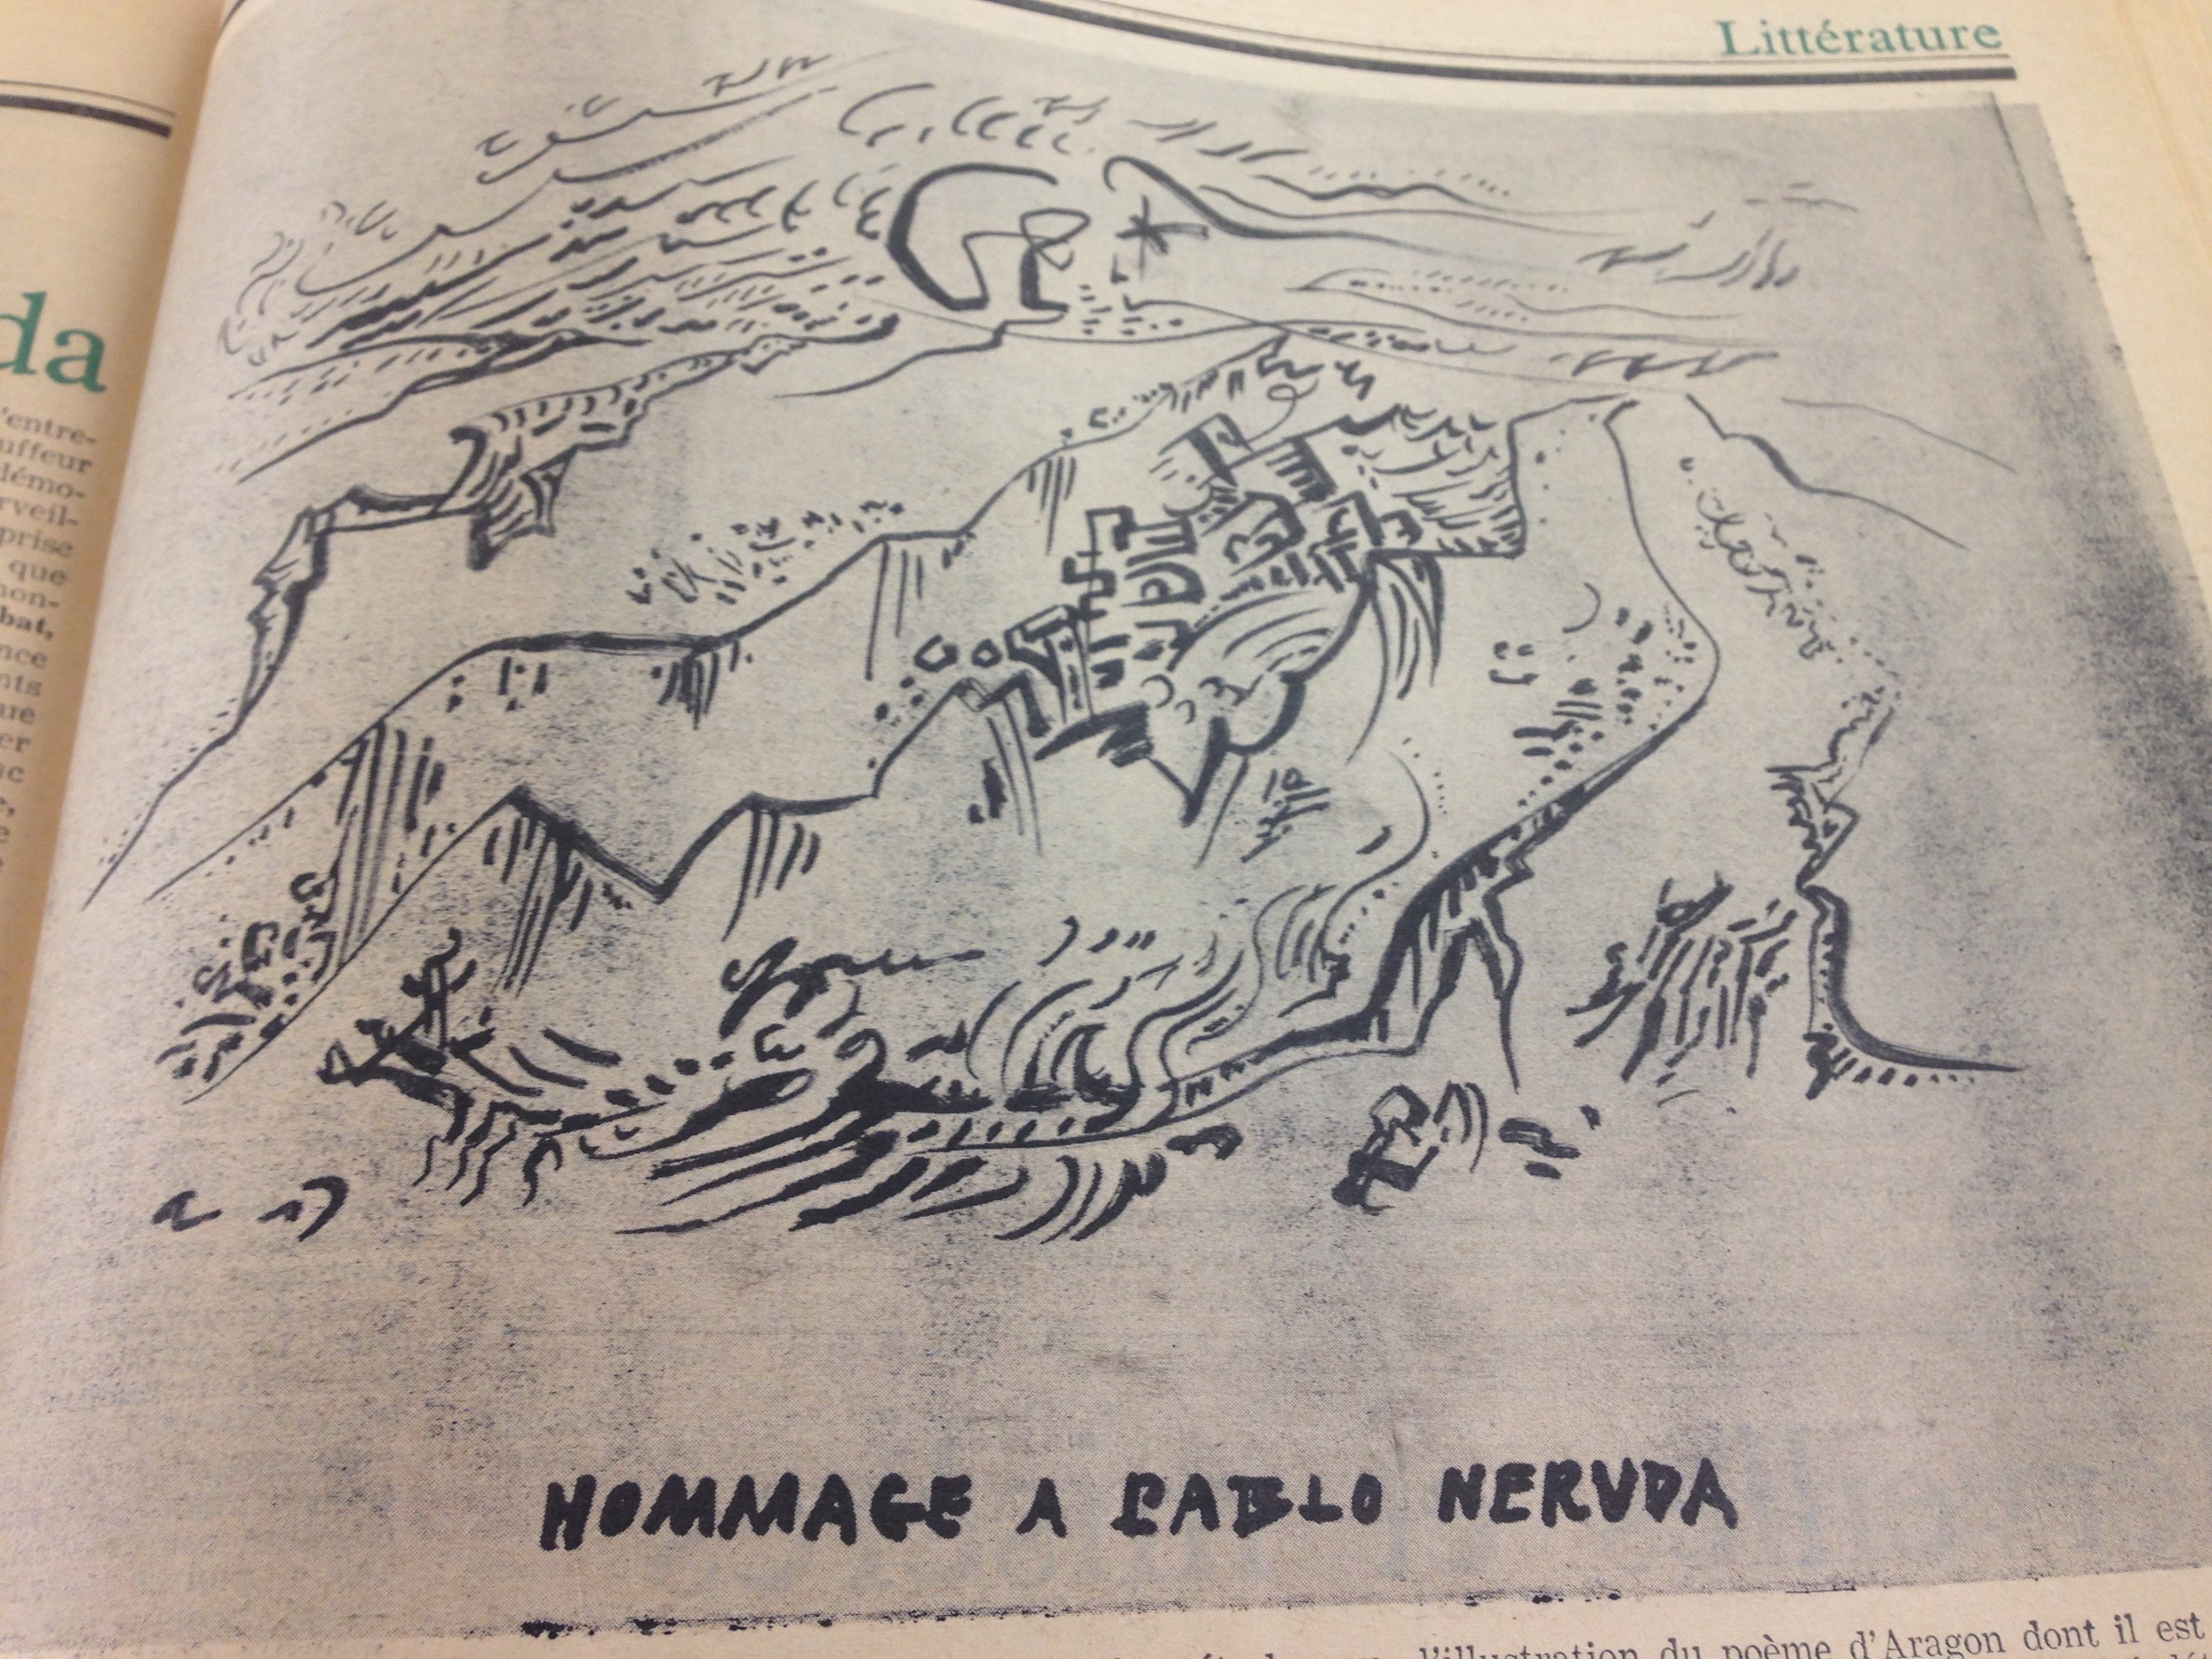
\includegraphics[width=0.33\textwidth]{esquissen1108.jpg}
	\caption{\cite{pabloneruda}}\label{fig:MassonNeruda}
\end{figure}

	Cette esquisse-ci paraît vaste comme dans un plan d’ensemble, avec de longs traits étendus et écartés les uns des autres. Les traits du premier plan, les plus épais, verticaux et parallèles les uns aux autres se rejoignent vers le centre- haut du dessin pour former ce qui se rapprocherait d’un triangle : C’est donc d’abord à une montagne que les lignes auraient pour évocation en premier lieu, mais pas seulement. Mais, à observer l’esquisse en détail, certaines de ces lignes verticales et courbées forment dans leur élan parallèle la forme d’un oiseau. 


En outre, l’esquisse est riche de petits personnages, sous une forme minimaliste, certains mêmes entre la figuration et le trait pur. Le plus visible d’entre eux se situe au sommet de l’esquisse, les bras faits de petits et fins traits en direction de l’étoile. Or, si la jambe droite du personnage prend appui sur le trait de la montagne, sa jambe gauche est une courbe épaisse autour de son corps, d’une forme similaire à la lune. Ce personnage en hauteur dans les astres au corps composé en partie d’un astre lunaire aux côtés de l’étoile rappelle dans l’imaginaire de Masson la figure du poète. Ainsi, Aragon et Masson dans cette collaboration entremêlent à la fois l’hommage au Chili et au poète qu’est Neruda, avec un même élan lyrique vers une dimension onirique. Par ailleurs, cette représentation commune chez Aragon et Masson rejoint celle argumentée par Jean Marcenac dans son étude :

\begin{quote}
Neruda est ainsi parmi nous un homme qui rattache l’homme à la fois aux autres hommes et au monde. Et c’est parce que le lien qu’il noue est ainsi double qu’il est si puissant, indissoluble. L’apport immense de Neruda, dans la poésie d’aujourd’hui se ramène à cette affirmation jumelle : qu’il n’est de poésie que de l’homme - ce que nous savions - et qu’il n’est d’homme que de la terre - ce que peut-être un certain \enquote{humanisme} nous avait fait oublier.\footcite[p119]{pabloneruda}\end{quote}

Cette notion de terre, tout comme la lumière, constitue d’ailleurs les grands thèmes de la poésie de Neruda. C’est également cette double filiation décrite par Marcenac que révèlent Aragon par le biais de l’imagerie poétique, Masson par le dessin. Ainsi, le Chili évoque simultanément à a terre le poète lui même : \enquote{Au Chili les cerises dansent, / les obscures jeunes filles chantent, / et l'eau brille sur les guitares.}\footcite{pabloneruda} Dans cette troisième strophe du Paresseux, le poète Aragon voit la terre chilienne avec les yeux de Neruda lui-même, et c’est ce lyrisme qui le pousse à cette affirmation au vers final : \enquote{Je ne veux pas changer de planète}\footcite{pabloneruda}.  On ne peut exclure une certaine forme de résistance chez le poète accompagné par un lyrisme des terres chiliennes : \emph{Le Paresseux }ne part pas après le tremblement de terre, il se sent encore rattaché à cette terre chilienne. L’esquisse d’André Masson rejoint cette image du poète littéralement composé du monde, avec ce petit bonhomme fait en partie d’astres et donc le corps composé de lignes se mêle à celles du tremblement de terre auquel la légende appellerait à signifier ainsi ces lignes courbes verticales à la formes triangulaires proches de la montagne. Tous les personnes qui gravitent autour du tremblement, et parfois entraperçus par des fragments de corps à l’intérieur même du tremblement de terre en train de jaillir dans l’élan vif des lignes, sont en réalité des compositions du tremblement de terre en train de jaillir. 



	En outre, la figure confondue dans \emph{Le Paresseux}, de la terre et du poète évoque d’une part le souci de transtextualité cher à Aragon, à savoir mêler à ses vers ceux de Pablo Neruda. C’est pourquoi, à la fin de son recueil \emph{Le Nouveau Crève-Coeur}, Aragon mêlait déjà ces deux figures, à tel point que relire ces poèmes en hommage à Neruda révèle des figures qui semblent annoncer le terrible événement, bien que ce soit le topos du feu qui soit le plus récemment associé au poète Neruda : 



\begin{verse}
A Madrid il est consul 
En trente-six quand le feu
Change sur la péninsule
En ciel rouge le ciel bleu\footcite{pabloneruda}	
\end{verse}
 
	La scène décrite est ambiguë : La description annoncerait un contexte apocalyptique, digne du réel tremblement de terre dévastateur quelques années plus tard, et pourtant c’est aussi exactement le contraire que sous-entendent les références absolues et la figure d’autorité de \enquote{consul}attribuée à Neruda. Et peut-être aussi l’affection manifestée par Aragon dans cette \emph{Complainte à Pablo Neruda} qui rend plus plausible l’hypothèse d’un changement positif attribué à Neruda du changement de l’atmosphère politique en Espagne. Aragon va même à faire de Neruda la figure d’autorité qui aurait commandité la transition insurrectionnelle de trente-six depuis la proclamation de la 1ère République du 14 avril 1936. Ainsi, le feu a priori dévastateur est aussi la force tant poétique qu’insurrectionnelle du poète Neruda avide de liberté. Or, c’est aussi cette même liberté qu’Aragon prête à la maison du poète, associée à la figure féminine. C’est même cette tournure lyrique finale qui convoque l’image de la figure féminine mais aussi comme la \emph{Passante} de Baudelaire, c’est-à-dire un motif de liberté en sens le plus large, et d’autant plus totale qu’elle se compose d’éléments éphémères. Devant cet entremêlement de la Beauté incarnée par la femme et de la liberté, à l’image des éléments naturels tels que le tremblement de terre qui emporte la maison, le lyrisme de l’atmosphère suffit à justifier l’affirmation en strophe finale : \enquote{Je ne veux pas changer de planète.}\footcite{pabloneruda}

Ainsi, André Masson et Pablo Neruda partagent cette fascination essentielle dans leur oeuvre d’une image du mouvement pris sur le vif, dans le jaillissement de l’expression en train de devenir. En somme, le poème \emph{Le Paresseux} d’Aragon comme l’esquisse de Masson s’attachent non au tremblement en tant que catastrophe, mais comme portrait lyrique du poète Neruda, et des hommes en général comme ses propres poèmes s’y vouent : L’identité inconsistante et en perpétuelle composition de l’homme.



    \chapter*{Conclusion} \markboth{Conclusion}{Conclusion}

L'aventure du lyrisme révolutionnaire dans les numéros des \emph{Lettres françaises} entre Aragon et André Masson s'inscrit plus largement dans la réactualisation de l'amitié de ces deux hommes, tous deux âgés et perçus mutuellemet comme les survivants des grands mouvements de leur jeunesse. Tandis que depuis les années 1960 se multiplient les hommages de leurs amis du groupe surréalsites disparus, l'un et l'autre affichent leur amitié, et avec elle leurs croisements idéologiques et esthétiques, principalement autour de collaborations d'hommages. La qualité d'hommage pour un tiers, un être cher en commun, n'omet en rien l'importance des retrouvailles de cex des hommes au destins croisés sur bien des aspects. A commencer par le passé sur le champ de bataille durant la 1ère Guerre Mondiale, mais dont déjà la différence de psote, donc d'expérience, de l'un et de l'autre représente quelles proximités Aragon et Masson connaissent dans leurs parcorus respectifs, tout en se ditinguant par une orientation idéologique différente. Les premières grandes collaborations entre Aragon et André Masson commencent dans la transition entre dada et le surréalisme pour Aragon, lorsqu'il rencontre les artistes de la rue Blomet, et que ses collaborations telles \emph{Le Con d'Irène  } en 1928 avec André Masson s'attèlent à la recherche de l'exepression la plus libre possible, exprimée par l'érotisme. Mais ce n'est sans doute pas un hasard si le Aragon romancier et directeur de journal dans les années 1960 prolonge les recherches esthétiques et idéologique de ses jeunes années surréalsites dans une perspective qui croise celles de Masson. Avec des collaborations d'hommage de sortes très diverses, de la mort de Georges Limbour, l'une des grandes figures médiatrices entre eux à l'origine de leur rencontre, jusqu'à l'hommage à Pablo Neruda lui bien vivant en raison de l'explosion de sa maison, sans compter les articles cette fois en l'honneur de Masson ou ceux d'Aragon et de Masson dont les associations d'idées s'entremêlent d'un numéro à l'autre, \emph{Les Lettres françaises} devient le lieu polyphonique de ce nouveau temps d'amitié. 

Les temps d'apparente perte de contact, ou tout du moins d'échanges plus discrets sont également évocateurs, et le rapport au lyrisme révolutionnaire de l'un et de l'autre en manifeste un exemple symbolique:la sensiblité de l'un et de l'autre pour la Commune de Paris l'illustre en profondeur, puisqu'elle constiute un moment historique qui influence directement le projet romanesque et journalsitique d'Aragon et l'art de Masson. Cependant, aussitôt ce point commun fort formulé, les distinctions politiques de l'un et de l'autre ne permet pas la fusion complète autour du lyrisme révolutionnaire qu'incarne pourtant la Commune dans leur imaginaire. La cause en revient à leur distinction idéologique, en particulier lorsqu'Aragon quitte le groupe surréaliste pour le parti communiste, tandis que Masson non seulement refuse ce rapport militant vis-à-vis d'un parti, et surtout considérant les thèses marxistes comme des formes de servitude de l'homme. Pourtant, philosphiquement parlant, Aragon et André Masson ne font que rechercher cette liberté totale déjà entrevue dans leurs premières collaborations. 

    \newpage
    
    \addcontentsline{toc}{chapter}{Table des Matières}
    \tableofcontents
    
    \newpage
    
    \addcontentsline{toc}{chapter}{Bibliographie}
    \printbibliography{}
    
\end{document}